% \iffalse
%
% Copyright 2016-2020, Association for Computing Machinery
% This work may be distributed and/or modified under the
% conditions of the LaTeX Project Public License, either
% version 1.3 of this license or (at your option) any
% later version.
% The latest version of the license is in
%    http://www.latex-project.org/lppl.txt
% and version 1.3 or later is part of all distributions of
% LaTeX version 2005/12/01 or later.
%
% This work has the LPPL maintenance status `maintained'.
%
% The Current Maintainer of this work is Boris Veytsman,
% <borisv@lk.net>
%
% This work consists of the file acmart.dtx, the derived file
% acmart.cls, the files ACM-Reference-Format.bst, and templates
% sample-acmlarge.tex, sample-acmsmall.tex, sample-acmtog.tex,
% samplebody-conf.tex, samplebody-journals.tex, sample-manuscript.tex,
% sample-sigconf-authordraft.tex, sample-sigconf.tex,
% sample-sigplan.tex
%
% \fi
%
%
%% \CharacterTable
%%  {Upper-case    \A\B\C\D\E\F\G\H\I\J\K\L\M\N\O\P\Q\R\S\T\U\V\W\X\Y\Z
%%   Lower-case    \a\b\c\d\e\f\g\h\i\j\k\l\m\n\o\p\q\r\s\t\u\v\w\x\y\z
%%   Digits        \0\1\2\3\4\5\6\7\8\9
%%   Exclamation   \!     Double quote  \"     Hash (number) \#
%%   Dollar        \$     Percent       \%     Ampersand     \&
%%   Acute accent  \'     Left paren    \(     Right paren   \)
%%   Asterisk      \*     Plus          \+     Comma         \,
%%   Minus         \-     Point         \.     Solidus       \/
%%   Colon         \:     Semicolon     \;     Less than     \<
%%   Equals        \=     Greater than  \>     Question mark \?
%%   Commercial at \@     Left bracket  \[     Backslash     \\
%%   Right bracket \]     Circumflex    \^     Underscore    \_
%%   Grave accent  \`     Left brace    \{     Vertical bar  \|
%%   Right brace   \}     Tilde         \~}
%
%
% \MakeShortVerb{|}
% \def\guide{acmguide}
% \iffalse
% From
% http://tex.stackexchange.com/questions/117892/can-i-convert-a-string-to-catcode-11 by egreg
% \fi
% \begingroup
%  \everyeof{\noexpand}
%  \endlinechar=-1
%  \xdef\currentjob{\scantokens\expandafter{\jobname}}
% \endgroup
%
% \ifx\currentjob\guide\OnlyDescription\fi
% \GetFileInfo{acmart.dtx}
% \title{\LaTeX{} Class for the \emph{Association for Computing
% Machinery}\thanks{\copyright 2016--2020, Association for Computing Machinery}}
% \author{Boris Veytsman\thanks{%
% \href{mailto:borisv@lk.net}{\texttt{borisv@lk.net}},
% \href{mailto:boris@varphi.com}{\texttt{boris@varphi.com}}}}
% \date{\filedate, \fileversion}
% \maketitle
% \begin{abstract}
%   This package provides a class for typesetting publications of
%   the Association for Computing Machinery.
% \end{abstract}
% \tableofcontents
%
% \clearpage
%
%\section{Introduction}
%\label{sec:intro}
%
% The Association for Computing
% Machinery\footnote{\url{http://www.acm.org/}} is the world's largest
% educational and scientific computing society, which delivers
% resources that advance computing as a science and a
% profession.  It was one of the
% early adopters of \TeX\ for its typesetting.
%
% It provided several different classes for a number of journals and
% conference proceedings.  Unfortunately during the years since these
% classes were written, the code was patched many times, and
% supporting different versions of the classes became difficult.
%
% This package provides the uniform interface for all ACM
% publications.  It is intended to replace all the different classes and
% packages and provide an up-to-date \LaTeX\ package.
%
% This package uses only free \TeX\ packages and fonts included in \TeX
% Live, Mik\TeX\ and other popular \TeX\ distributions.  It is
% intended to be published in these distributions itself, which
% minimizes users' efforts in the installation and support of this
% package.
%
%  I am grateful to
%  Michael D.~Adams,
%  Leif Andersen,
%  Lawrence Christopher Angrave,
%  Dirk Beyer,
%  Andrew Black,
%  Joachim Breitner,
%  Benjamin Byholm,
%  Nils Anders Danielsson,
%  Michael Ekstrand,
%  Matthew Fluet,
%  Paolo G.~Giarrusso,
%  Ben Greenman,
%  Enrico Gregorio,
%  Jamie Davis,
%  Jason Hemann,
%  Peter Kemp,
%  Luis Leiva,
%  Ben Liblit,
%  Rholais Lii,
%  LianTze Lim,
%  Kai Mindermann,
%  Frank Mittelbach,
%  Serguei Mokhov,
%  Ross Moore,
%  John Owens,
%  Joel Nider,
%  Tobias Pape,
%  Philip Quinn,
%  Mathias Rav,
%  Andreas Reichinger,
%  Matteo Riondato,
%  Craig Rodkin,
%  Bernard Rous,
%  Feras Saad,
%  Kerry A. Seitz, Jr.,
%  David Shamma,
%  Gabriel Scherer,
%  Kartik Singhal,
%  Stephen Spencer,
%  Shin Hwei Tan,
%  Daniel Thomas,
%  Shari Trewin,
%  Zack Weinberg,
%  John Wickerson
%  and many others for their invaluable help.
%
% The development version of the package is available at
% \url{https://github.com/borisveytsman/acmart}.
%
%\section{User's guide}
%\label{sec:ug}
%
%
% This class uses many commands and customizaton options, so it might
% appear intimidating for a casual user.  Do not panic!  Many of these
% commands and options can be safely left with their default values
% or the values recommended by your conference or journal editors.  If
% you have problems or questions, do not hesitate to ask me directly
% or the community at \url{https://github.com/borisveytsman/acmart},
% \url{https://tex.stackexchange.com} or the closest \TeX\ Users
% Group.  The world-wide \TeX\ Users Group is at
% \url{https://tug.org/}; please consider joining us if you use \TeX\
% regularly.
%
%\subsection{Installation}
%\label{sec:ug_install}
%
% Most probably, you already have this package installed in your
% favorite \TeX\ distribution;  if not, you may want to upgrade.  You
% may need to upgrade it anyway since this package uses a number of
% relatively recent packages, especially the ones related to fonts.
%
% The latest released version of this package can be found on CTAN:
% \url{https://www.ctan.org/pkg/acmart}.   The development version can
% be found on GitHub: \url{https://github.com/borisveytsman/acmart}.
% At this address you can file a bug report---or even contribute your
% own enhancement by making a pull request.
%
% Please note that the version on Github is a development (or
% experimental) version: please download it for testing new features.
% The production version is the one on CTAN and ACM sites.
%
% Most users should not attempt to install this package themselves
% but should rather rely on their \TeX\ distributions to provide it.  If you
% decide to install the package yourself, follow the standard rules:
% \begin{enumerate}
% \item Run |latex acmart.ins|.  This will produce the file
% |acmart.cls|
% \item Put the files |acmart.cls| and |ACM-Reference-Format.bst|
%   in places where \LaTeX{} can find them (see \cite{TeXFAQ} or
%   the documentation for your \TeX{} system).\label{item:install}
% \item Update the database of file names.  Again, see \cite{TeXFAQ}
% or the documentation for your \TeX{} system for the system-specific
% details.\label{item:update}
% \item The file |acmart.pdf| provides the documentation for the
% package.  (This is probably the file you are reading now.)
% \end{enumerate}
% As an alternative to items~\ref{item:install} and~\ref{item:update}
% you can just put the files in the working directory where your
% |.tex| file is.
%
%
% This class uses a number of other packages.  They are included in all
% major \TeX\ distributions (\TeX Live, Mac\TeX, Mik\TeX) of 2015 and
% later, so you probably have them installed.  Just in case here is
% the list of these packages:
% \begin{itemize}
% \item \textsl{amscls}, \url{http://www.ctan.org/pkg/amscls}
% \item \textsl{amsfonts}, \url{http://www.ctan.org/pkg/amsfonts}
% \item \textsl{amsmath}, \url{http://www.ctan.org/pkg/amsmath}
% \item \textsl{binhex}, \url{http://www.ctan.org/pkg/binhex}
% \item \textsl{balance}, \url{http://www.ctan.org/pkg/balance}
% \item \textsl{booktabs}, \url{http://www.ctan.org/pkg/booktabs}
% \item \textsl{caption}, \url{http://www.ctan.org/pkg/caption}
% \item \textsl{comment}, \url{http://www.ctan.org/pkg/comment}
% \item \textsl{cm-super}, \url{http://www.ctan.org/pkg/cm-super}
% \item \textsl{cmap}, \url{http://www.ctan.org/pkg/cmap}
% \item \textsl{draftwatermark}, \url{http://www.ctan.org/pkg/draftwatermark}
% \item \textsl{environ}, \url{http://www.ctan.org/pkg/environ}
% \item \textsl{etoolbox}, \url{http://www.ctan.org/pkg/etoolbox}
% \item \textsl{fancyhdr}, \url{http://www.ctan.org/pkg/fancyhdr}
% \item \textsl{float}, \url{http://www.ctan.org/pkg/float}
% \item \textsl{fontaxes}, \url{http://www.ctan.org/pkg/fontaxes}
% \item \textsl{geometry}, \url{http://www.ctan.org/pkg/geometry}
% \item \textsl{graphics}, \url{http://www.ctan.org/pkg/graphics}
% \item \textsl{hyperref}, \url{http://www.ctan.org/pkg/hyperref}
% \item \textsl{iftex}, \url{http://www.ctan.org/pkg/iftex}
% \item \textsl{inconsolata}, \url{http://www.ctan.org/pkg/inconsolata}
% \item \textsl{libertine}, \url{http://www.ctan.org/pkg/libertine}
% \item \textsl{manyfoot}, \url{http://www.ctan.org/pkg/manyfoot}
% \item \textsl{microtype}, \url{http://www.ctan.org/pkg/microtype}
% \item \textsl{mmap}, \url{http://www.ctan.org/pkg/mmap}
% \item \textsl{ms}, \url{http://www.ctan.org/pkg/ms}
% \item \textsl{mweights}, \url{http://www.ctan.org/pkg/mweights}
% \item \textsl{natbib}, \url{http://www.ctan.org/pkg/natbib}
% \item \textsl{nccfoots}, \url{http://www.ctan.org/pkg/nccfoots}
% \item \textsl{newtx}, \url{http://www.ctan.org/pkg/newtx}
% \item \textsl{oberdiek}, \url{http://www.ctan.org/pkg/oberdiek}
% \item \textsl{pdftex-def}, \url{http://www.ctan.org/pkg/pdftex-def}
% \item \textsl{refcount}, \url{http://www.ctan.org/pkg/refcount}
% \item \textsl{setspace}, \url{http://www.ctan.org/pkg/setspace}
% \item \textsl{textcase}, \url{http://www.ctan.org/pkg/textcase}
% \item \textsl{totpages}, \url{http://www.ctan.org/pkg/totpages}
% \item \textsl{trimspaces}, \url{http://www.ctan.org/pkg/trimspaces}
% \item \textsl{upquote}, \url{http://www.ctan.org/pkg/upquote}
% \item \textsl{url}, \url{http://www.ctan.org/pkg/url}
% \item \textsl{xcolor}, \url{http://www.ctan.org/pkg/xcolor}
% \item \textsl{xkeyval}, \url{http://www.ctan.org/pkg/xkeyval}
% \item \textsl{xstring}, \url{http://www.ctan.org/pkg/xstring}
% \end{itemize}
%
%
%\subsection{Invocation and options}
%\label{sec:invocation}
%
% To use this class, put in the preamble of your document
% \begin{quote}
%   \cs{documentclass}\oarg{options}|{acmart}|
% \end{quote}
% There are several options corresponding to the type of the document and
% its general appearance.  They are described below.  Generally
% speaking, the options have |key=value| forms, for example,
% \begin{verbatim}
% \documentclass[format=acmsmall, screen=true, review=false]{acmart}
% \end{verbatim}
%
%
% The option |format| describes the format of the output.  There are
% several possible values for this option, for example,
% \begin{verbatim}
%   \documentclass[format=acmtog]{acmart}
% \end{verbatim}
% Actually the words |format=| can be omitted, e.g.,
% \begin{verbatim}
%   \documentclass[acmtog, review=false]{acmart}
% \end{verbatim}
% The possible formats are listed in
% Table~\ref{tab:opts_format}.  Note that formats starting with |acm|
% are intended for journals and transactions, while formats starting
% with |sig| are intended for proceedings published as books.
%
% Note that sometimes conference proceedings are published as a
% special issue (or issues) of an ACM journal.  In this case, you
% should use the journal format for a conference paper.  Please
% contact your conference committee if in doubt.
%
% \begin{table}
%   \centering
%   \caption{The possible values for the \texttt{format} option}
%   \label{tab:opts_format}
%   \begin{tabularx}{\textwidth}{>{\ttfamily}lX}
%     \toprule
%     \normalfont Value & Meaning\\
%     \midrule
%   manuscript & A manuscript. This is the default. \\
%   acmsmall & Small single-column format.  Used for CIE, CSUR, 
%            JACM, JDIQ, JEA, JERIC,
%            JETC, PACMCGIT, PACMHCI, PACMPL, TAAS, TACCESS, TACO,
%            TALG, TALLIP (formerly TALIP), TCPS, TDS,
%            TEAC, TECS, TELO, THRI, TIIS, TIOT, TISSEC, TIST, TKDD, TMIS,
%            TOCE, TOCHI, TOCL,
%            TOCS, TOCT, TODAES, TODS, TOIS, TOIT, TOMACS, TOMM (formerly
%            TOMCCAP), TOMPECS, TOMS, TOPC, TOPLAS, TOPS,
%            TOS, TOSEM, TOSN, TQC, TRETS,
%            TSAS, TSC, TSLP and TWEB, including special issues. \\
%   acmlarge  & Large single-column format.  Used for DTRAP, HEALTH,
%           IMWUT, JOCCH, POMACS and TAP, including special issues. \\
%   acmtog   & Large double-column format.  Used for
%          TOG, including annual conference Technical Papers.\\
%   sigconf & Proceedings format for most ACM
%          conferences (with the exceptions listed below) and all ICPS
%          volumes.\\
%   sigplan & Proceedings format for SIGPLAN conferences.\\
%   \bottomrule
%   \end{tabularx}
% \end{table}
%
% Starting in 2020, ACM retired formats |sigchi| and |sigchi-a|.
% SIGCHI conferences now use |sigconf| format for their publications.
% If a file uses |sigchi| format, a warning is issued, and the format
% is automatically switched to |sigconf|.  Format |sigchi-a| can be
% used for non-ACM documents only (see Section~\ref{sec:sigchi-a}).  
%
% There are several Boolean options that can take |true| or |false|
% values.  They are listed in Table~\ref{tab:opts_bool}.  The words
% |=true| can be omitted when setting a Boolean option, so instead of
% |screen=true| one can write just |screen|, for example,
% \begin{verbatim}
% \documentclass[acmsmall, screen, review]{acmart}
% \end{verbatim}
% The option |review| is useful when combined with the |manuscript| format
% option.  It provides a version suitable for reviewers and
% copy editors.
%
% The default for the option |screen| depends on the publication.  At
% present it is |false| for all publications \emph{but} PACM, since
% PACM is now electronic-only.  Thus PACM titles~(see
% Table~\ref{tab:pubs}) set this option to |true|.  In the future this
% option may involve additional features suitable for on-screen
% versions of articles.
%
% The option |natbib| is used when the corresponding
% \BibTeX\ style is based on |natbib|.  In most cases you do not need
% to set it.  See
% Section~\ref{sec:ug_bibliography}.
%
% The option |anonymous| is used
% for anonymous review processes and causes all author information to be
% obscured.
%
% The option |timestamp| is used to include a time stamp in the
% footer of each page.  When preparing a document, this can help avoid
% confusing different revisions.  The footer also includes the page range of
% the document.  This helps detect missing pages in hard copies.
%
% The option |authordraft| is intended for author's drafts that are not
% intended for distribution.  It typesets a copyright block to give the
% author an idea of its size and the overall size of the paper but
% overprints it with the phrase ``Unpublished working draft. Not for
% distribution.'', which is also used as a watermark.  This option sets
% |timestamp| and |review| to |true|, but these can be
% overriden by setting these options to |false| \emph{after}
% setting |authordraft| to |true|.
%
% The option |balance| determines whether the last page in the two
% column mode has balanced columns.  By default it is |true|; however,
% it may lead to problems for some documents.  Set it to |false| if
% you encounter compilation errors.  Note that for one page documents
% \cs{balance} command might cause problems.
%
% The option |urlbreakonhyphens| determines whether URLs can be split
% between lines after hyphens.  By default it is true.  Set it to
% |false| to disallow these breaks.
%
% \begin{table}
%   \centering
%   \caption{Boolean options}
%   \label{tab:opts_bool}
%   \begin{tabularx}{\textwidth}{>{\ttfamily}l>{\ttfamily}lX}
%     \toprule
%     \normalfont Option & \normalfont Default & Meaning\\
%     \midrule
%     review & false & A review version: lines are numbered and
%     hyperlinks are colored\\
%     screen & {\rmfamily see text} & A screen version:
%     hyperlinks are colored\\
%     natbib & true & Whether to use the |natbib| package (see
%     Section~\ref{sec:ug_bibliography})\\
%     anonymous & false & Whether to make author(s) anonymous\\
%     authorversion & false & Whether to generate a special
%     version for the authors' personal use or posting (see
%     Section~\ref{sec:ug_topmatter})\\
%     nonacm & false & Use the class typesetting options for
%     a non-ACM document, which will not include the conference/journal
%     header and footers or permission statements\\
%     timestamp & false & Whether to put a time stamp in the
%     footer of each page\\
%     authordraft & false & Whether author's-draft mode is enabled\\
%     acmthm & true & Whether to define theorem-like environments, see
%                       Section~\ref{sec:ug_theorems}\\
%     balance & true & Whether to balance the last page in two column
%                        mode\\
%     urlbreakonhyphens & true & Whether to break urls on hyphens\\ 
%     \bottomrule
%   \end{tabularx}
% \end{table}
%
%
%
%\subsection{Top matter}
%\label{sec:ug_topmatter}
%
% A number of commands set up \emph{top matter} or (in
% computer science jargon) \emph{metadata} for an article.  They
% establish the publication name, article title, authors, DOI and
% other data.  Some of these commands, like \cs{title} and \cs{author},
% should be put by the authors.  Others, like \cs{acmVolume} and
% \cs{acmDOI}---by the editors.  Below we describe these commands and
% mention who should issue them.  These macros should be used
% \emph{before} the \cs{maketitle} command.  Note that in previous
% versions of ACM classes some of these commands should be used before
% \cs{maketitle}, and some after it. Now they all must be used before
% \cs{maketitle}.
%
%
% This class internally loads the |amsart| class, so many top-matter
% commands are inherited from |amsart|~\cite{Downes04:amsart}.
%
% \DescribeMacro{\acmJournal}%
% The macro \cs{acmJournal}\marg{shortName} sets the name of the
% journal or transaction for journals and transactions.  The argument
% is the short name of the publication \emph{in uppercase}, for
% example,
% \begin{verbatim}
% \acmJournal{TOMS}
% \end{verbatim}
% The currently recognized journals are listed in
% Table~\ref{tab:pubs}.  Note that conference proceedings published in
% \emph{book} form do not set this macro.
%
%
%
% \DescribeMacro{\acmConference}%
% The macro
% \cs{acmConference}\oarg{short name}\marg{name}\marg{date}\marg{venue} is
% used for conference proceedings published in the book form.  The
% arguments are the following:
% \begin{description}
% \item[short name:] the abbreviated name of the conference (optional).
% \item[name:] the name of the conference.
% \item[date:] the date(s) of the conference.
% \item[venue:] the place of the conference.
% \end{description}
% Examples:
% \begin{verbatim}
% \acmConference[TD'15]{Technical Data Conference}{November
% 12--16}{Dallas, TX, USA}
% \acmConference{SA'15 Art Papers}{November 02--06, 2015}{Kobe, Japan}
% \end{verbatim}
%
% \DescribeMacro{\acmBooktitle}%
% By default we assume that conference proceedings are published
% in the book named \emph{Proceedings of \textsc{CONFERENCE}}, where
% \textsc{CONFERENCE} is the name of the conference inferred from the
% command \cs{acmConference} above.  However, sometimes the book title
% is different.  The command \cs{acmBooktitle} can be used to set this
% title, for example,
% \begin{verbatim}
% \acmBooktitle{Companion to the first International Conference on the
% Art, Science and Engineering of Programming (Programming '17)}
% \end{verbatim}
%
% An ACM paper should have either \cs{acmJournal} or
% \cs{acmConference} command.  If it has both (or more) commands, the
% last one takes precedence.  Note that if you have the command
% \cs{acmConference} in a journal format like |acmsmall|, the class
% will use conference format for bibstrip and reference citation
% formatting.  In the samples directory there is a file
% |sample-acmsmall-conf.tex| with the example of this usage.
%
% 
%
% \DescribeMacro{\editor}%
% In most cases, conference proceedings are edited.  You can use the
% command \cs{editor}\marg{editor} to set the editor of the volume.
% This command can be repeated, for example,
% \begin{verbatim}
% \editor{Jennifer B. Sartor}
% \editor{Theo D'Hondt}
% \editor{Wolfgang De Meuter}
% \end{verbatim}
%
%
% \DescribeMacro{\title}%
% The command |\title|, as in the |amsart| class, has two arguments:  one
% optional, and one mandatory:
% \begin{flushleft}
%   |\title[|\meta{ShortTitle}|]{|\meta{FullTitle}|}|
% \end{flushleft}
% The mandatory argument is the full title of the article.  The
% optional argument, if present, defines the shorter version of the
% title for running heads.  If the optional argument is absent, the
% full title is used instead.
%
% It is expected that this command is inserted by the author of the
% manuscript.
%
% \DescribeMacro{\subtitle}%
% Besides title, ACM classes allow a subtitle, set with the
% \cs{subtitle}\marg{subtitle} macro.
%
% The commands for specifying authors are highly structured.
% The reason is they serve double duty:  the authors' information is
% typeset in the manuscript \emph{and} is used by the metadata
% extraction tools for indexing and cataloguing.  Therefore it is very
% important to follow the guidelines exactly.
%
% \DescribeMacro{\author}%
% \DescribeMacro{\orcid}
% \DescribeMacro{\affiliation}%
% \DescribeMacro{\email}%
% The basic commands are \cs{author}, \cs{orcid} (for the researchers
% registered with ORCID, \url{http://www.orcid.org/}), \cs{affiliation} and
% \cs{email}.  In the simplest case, you enter them in this order:
% \begin{verbatim}
% \author{...}
% \orcid{...}
% \affiliation{...}
% \email{...}
% \end{verbatim}
% Do \emph{not} use the \LaTeX\ \cs{and} macro or commas, or \verb|\\|
% between the authors! Each author deserves his or
% her own \cs{author} command.  An attempt to list several authors or
% their e-mails in one command leads to a warning or an error.  This
% is not a bug, but the expected behavior.
%
% Note that some formats do not typeset e-mails or ORCID identifiers.
% Do not worry: the metadata tools will get them.
%
% Sometimes an author has several affiliations.  In this case, the
% \cs{affiliation} command should be repeated:
% \begin{verbatim}
% \author{...}
% \orcid{...}
% \affiliation{...}
% \affiliation{...}
% \email{...}
% \end{verbatim}
% Similarly you can repeat the \cs{email} command.
%
% You may have several authors with the same affiliation, different
% affiliations, or overlapping affiliations (author~$A_1$ is affiliated
% with institutions $I_1$ and $I_2$, while author $A_2$ is affiliated
% with $I_2$ only, author $A_3$ is affiliated with
% $I_1$ and $I_3$, etc.).  The recommended solution is to put the
% \cs{affiliation} commands after each author, possibly repeating them:
% \begin{verbatim}
% \author{...}
% \orcid{...}
% \affiliation{...}
% \affiliation{...}
% \email{...}
% \author{...}
% \orcid{...}
% \affiliation{...}
% \email{...}
% \author{...}
% \orcid{...}
% \affiliation{...}
% \affiliation{...}
% \email{...}
% \end{verbatim}
%  In some cases, when several authors share the same affiliation, you can
%  try to save space using the format
% \begin{verbatim}
% \author{...}
% \email{...}
% \author{...}
% \email{...}
% \affiliation{...}
% \end{verbatim}
%  However, this format is not generally recommended.
%
% \DescribeMacro{\additionalaffiliation}%
% In some cases, too many affiliations can take too much space.  The
% command \cs{additionalaffiliation}\marg{affiliation} creates a
% footnote after an author's name with the words ``Also with
% \marg{affiliation}''.  You should use this command only as a last
% resort.  An example of usage is:
% \begin{verbatim}
% \author{G. Tobin}
% \author{Ben Trovato}
% \additionalaffiliation{%
%   \institution{The Th{\o}rv{\"a}ld Group}
%   \streetaddress{1 Th{\o}rv{\"a}ld Circle}
%   \city{Hekla}
%   \country{Iceland}}
% \affiliation{%
%   \institution{Institute for Clarity in Documentation}
%   \streetaddress{P.O. Box 1212}
%   \city{Dublin}
%   \state{Ohio}
%   \postcode{43017-6221}}
% \end{verbatim}
% Here Trovato and Tobin share their affiliation with the Institute
% for Clarity in Documentation, but only Ben Trovato is affiliated
% with The Th{\o}rv{\"a}ld Group.
%
%
% \DescribeMacro{\position}%
% \DescribeMacro{\institution}%
% \DescribeMacro{\department}%
% \DescribeMacro{\streetaddress}%
% \DescribeMacro{\city}%
% \DescribeMacro{\state}%
% \DescribeMacro{\postcode}%
% \DescribeMacro{\country}%
% The \cs{affiliation} and \cs{additionalaffiliation} commands are
% further structured to interact with the metadata extraction tools.
% Inside these commands you should use the \cs{position},
% \cs{institution}, \cs{department}, \cs{city}, \cs{streetaddress},
% \cs{state}, \cs{postcode} and \cs{country} macros to indicate the
% corresponding parts of the affiliation.  Note that in some cases
% (for example, journals) these parts are not printed in the resulting
% copy, but they \emph{are} necessary since they are used by the XML
% metadata extraction programs.  Do \emph{not} put commas or |\\|
% between the elements of \cs{affiliation}.  They will be provided
% automatically.  
%
%
% An example of the author block:
% \begin{verbatim}
% \author{A. U. Thor}
% \orcid{1234-4564-1234-4565}
% \affiliation{%
%   \institution{University of New South Wales}
%   \department{School of Biomedical Engineering}
%   \streetaddress{Samuels Building (F25), Kensington Campus}
%   \city{Sidney}
%   \state{NSW}
%   \postcode{2052}
%   \country{Australia}}
% \email{author@nsw.au.edu}
% \author{A. N. Other}
% \affiliation{%
%   \institution{University of New South Wales}
%   \city{Sidney}
%   \state{NSW}
%   \country{Australia}}
% \author{C. O. Respondent}
% \orcid{1234-4565-4564-1234}
% \affiliation{%
%   \institution{University of Pennsylvania}
%   \city{Philadelphia}
%   \state{PA}
%   \country{USA}}
% \affiliation{%
%   \institution{University of New South Wales}
%   \city{Sidney}
%   \state{NSW}
%   \country{Australia}}
% \end{verbatim}
%
% Note that the old ACM conference formats did not allow more than six
% authors and required some effort from authors to achieve
% alignment.  The new format is much better in this.
%
%  Sometimes an author works in several departments within the same
%  insitution.  There could be two situations: the departments are
%  independent, or one department is within another.  In the first
%  case, just repeat the command \cs{department} several times.  To
%  handle the second case the command has an optional numerical
%  parameter.  The departments with higher numbers are higher in the
%  organizational chart.  Compare
% \begin{verbatim}
% \affiliation{%
%   \department[0]{Department of Lunar Studies} % 0 is the default
%   \department[1]{John Doe Institute} % higher than 0
%   \institution{University of San Serriffe}
%   \country{San Serriffe}}
% \end{verbatim}
%  and
% \begin{verbatim}
% \affiliation{%
%   \department{Department of Lunar Studies} % Not in the John Doe Institute!
%   \department{John Doe Institute}
%   \institution{University of San Serriffe}
%   \country{San Serriffe}}
% \end{verbatim}
%
%
% The command \cs{affiliation} formats its output according to
% American conventions.  This might be wrong for some cases.
% Consider, for example, a German address.  In Germany, the postcode is
% put before the city and is not separated by a comma.  We can handle this
% order using
% \begin{verbatim}
% \affiliation{%
%   \institution{Fluginstitut}
%   \streetaddress{Sonnenallee 17}
%   \postcode{123456}
%   \city{Helm}
%   \country{Germany}}
% \end{verbatim}
% However, the comma after the postcode is unfortunate:  the address will
% be typeset (in some formats) as
% \begin{verbatim}
% Fluginstitut
% Sonenallee 17
% 123456, Helm, Germany
% \end{verbatim}
%
%
% To overcome this problem, the command \cs{affiliation} has an
% optional parameter |obeypunctuation|, which can be |false| (the
% default) or |true|.  If this parameter is |true|, \cs{afffiliation}
% obeys the author's command.  Thus
% \begin{verbatim}
% \affiliation[obeypunctuation=true]{%
%   \institution{Fluginstitut}\\
%   \streetaddress{Sonnenallee 17}\\
%   \postcode{123456}
%   \city{Helm},
%   \country{Germany}}
% \end{verbatim}
% will be typeset as
% \begin{verbatim}
% Fluginstitut
% Sonenallee 17
% 123456 Helm, Germany
% \end{verbatim}
%
% Note that you should \emph{not} use this option for journals.  
%
% It is expected that these commands are inserted by the author of the
% manuscript.
%
% \DescribeMacro{\thanks}%
% Like |amsart| (and unlike standard \LaTeX{}), we allow
% |\thanks| only \emph{outside} of the commands |\title| and |\author|.
% This command is obsolete and should \emph{not} be used in most
% cases.  Do not list your acknowledgments or grant sponsors here.
% Put this information in the |acks| environment (see
% Section~\ref{sec:ug_acks}).
%
% \DescribeMacro{\authorsaddresses}%
% In some formats, addresses are printed as a footnote on the first
% page.  By default \LaTeX\ typesets them itself using the information
% you give it.  However, you can override its choice using the
% commmand \cs{authorsaddresses}\marg{contact addresses}, for example,
% \begin{verbatim}
% \authorsaddresses{%
%  Authors' addresses: G.~Zhou, Computer Science Department, College of
%  William and Mary, 104 Jameson Rd, Williamsburg, PA 23185, US;
%  V.~B\'eranger, Inria Paris-Rocquencourt, Rocquencourt, France;
%  A.~Patel, Rajiv Gandhi University, Rono-Hills, Doimukh, Arunachal
%  Pradesh, India; H.~Chan, Tsinghua University, 30 Shuangqing Rd,
%  Haidian Qu, Beijing Shi, China; T.~Yan, Eaton Innovation Center,
%  Prague, Czech Republic; T.~He, C.~Huang, J.~A.~Stankovic University
%  of Virginia, School of Engineering Charlottesville, VA 22903, USA;
%  T. F. Abdelzaher, (Current address) NASA Ames Research Center,
%  Moffett Field, California 94035.}
% \end{verbatim}
% You can \emph{suppress} printing authors' addresses by setting them
% to an empty string:  |\authorsaddresses{}|.  Please note that
% authors' addresses are mandatory for journal articles.  
%
% \DescribeMacro{\titlenote}%
% \DescribeMacro{\subtitlenote}%
% \DescribeMacro{\authornote}%
% While the command \cs{thanks} generates a note without a footnote
% mark, sometimes the authors might need notes more tightly connected
% to the title, subtitle or author.  The commands \cs{titlenote},
% \cs{subtitlenote} and \cs{authornote} that follow the corresponding
% commands (\cs{title}, \cs{subtitle} and \cs{author}) generate such
% notes.  For example,
% \begin{verbatim}
% \title{This is a title}
% \titlenote{This is a titlenote}
% \author{A. U. Thor}
% \authornote{This is an authornote}
% \end{verbatim}
%
% Please never use a \cs{footnote} inside an \cs{author} or \cs{title}
% command since this confuses the metadata extraction software.  (Actually
% these commands now produce errors.)
%
% \DescribeMacro{\authornotemark}%
% Sometimes one may need to have the same footnote connected to
% several authors.  The command \cs{authornotemark}\oarg{number} adds
% just the footnote mark, for example,
% \begin{verbatim}
% \author{A. U. Thor}
% \authornote{Both authors contributed equally to the paper}
% ...
% \author{A. N. Other}
% \authornotemark[1]
% \end{verbatim}
% The correct numbering of these marks is the responsibility of the
% user.
%
% \DescribeMacro{\acmVolume}%
% \DescribeMacro{\acmNumber}%
% \DescribeMacro{\acmArticle}%
% \DescribeMacro{\acmYear}%
% \DescribeMacro{\acmMonth}%
% The macros \cs{acmVolume}, \cs{acmNumber}, \cs{acmArticle},
% \cs{acmYear} and \cs{acmMonth} are inserted by the editor and set
% the journal volume, issue, article number, year and month
% corrspondingly.  The arguments of all these commands, including
% \cs{acmMonth}, is numerical.  For example,
% \begin{verbatim}
% \acmVolume{9}
% \acmNumber{4}
% \acmArticle{39}
% \acmYear{2010}
% \acmMonth{3}
% \end{verbatim}
% Note that \cs{acmArticle} is used not only for journals but also
% for some conference proceedings.
%
% \DescribeMacro{\acmArticleSeq}%
% The articles in the same issue of a journal have a \emph{sequence
% number}.  It is used to vertically position the black blob on the first
% page of some formats.  By default it is the same as the article number,
% but the command \cs{acmArticleSeq}\marg{n} can be used to change it:
% \begin{verbatim}
% \acmArticle{39}   % The sequence number will be 39 by default
% \acmArticleSeq{5} % We redefine it to 5
% \end{verbatim}
% Setting this number to zero suppresses the blob.
%
% \DescribeMacro{\acmSubmissionID}%
% If your paper got a Submission~ID from the Conference Management
% System, put it here:
% \begin{verbatim}
% \acmSubmissionID{123-A56-BU3}
% \end{verbatim}
%
%
% \DescribeMacro{\acmPrice}%
% The macro \cs{acmPrice}\marg{price} sets the price for the article,
% for example,
% \begin{verbatim}
% \acmPrice{25.00}
% \end{verbatim}
% Note that you do not need to put the dollar sign here, just the
% amount.  By default the price is \$15.00, unless the copyright is
% set to |usgov|, |rightsretained|, |iw3c2w3|, or |iw3c2w3g|, when it
% is suppressed.  Note that to override the defaults you need to set
% the price \emph{after} the \cs{setcopyright} command.  Also, the
% command |\acmPrice{}| suppresses the printing of the price.
%
% \DescribeMacro{\acmISBN}%
% Book-like volumes have ISBN numbers attached to them.  The macro
% \cs{acmISBN}\marg{ISBN} sets it.  Normally it is set by the
% typesetter, for example,
% \begin{verbatim}
% \acmISBN{978-1-4503-3916-2}
% \end{verbatim}
% Setting it to the empty string, as |\acmISBN{}|, suppresses printing the
% ISBN.
%
% \DescribeMacro{\acmDOI}%
% The macro \cs{acmDOI}\marg{DOI} sets the DOI of the article, for
% example,
% \begin{verbatim}
% \acmDOI{10.1145/9999997.9999999}
% \end{verbatim}
% It is normally set by the typesetter.  Setting it to the empty
% string, as |\acmDOI{}|, suppresses the DOI.
%
%
% \DescribeMacro{\acmBadgeR}%
% \DescribeMacro{\acmBadgeL}%
% Some conference articles get special distinctions, for example, the
% artifact evaluation for PPoPP~2016
% (see~\url{http://ctuning.org/ae/ppopp2016.html}).  These articles
% display special badges supplied by the conference organizers.  This
% class provides commands to add these badges:
% \cs{acmBadgeR}\oarg{url}\marg{graphics} and
% \cs{acmBadgeL}\oarg{url}\marg{graphics}.  The first command puts the
% badge to the right of the title, and the second one---to the left.
% The arguments have the following meaning: \oarg{url}, if provided,
% sets the link to the badge authority in the screen version, while
% \marg{graphics} sets the graphics file with the badge image.  The
% file must be a cropped square, which is scaled to a standard size in
% the output.  For example, if the badge image is |ae-logo.pdf|, the
% command is
% \begin{verbatim}
% \acmBadgeR[http://ctuning.org/ae/ppopp2016.html]{ae-logo}
% \end{verbatim}
%
%
%
% \DescribeMacro{\startPage}%
% The macro \cs{startPage}\marg{page} sets the first page of the
% article in a journal or book.  It is used by the typesetter.
%
%
% \DescribeMacro{\terms}%
% \DescribeMacro{\keywords}%
% The command
% \cs{keywords}\marg{keyword, keyword,\ldots} sets keywords for the
% article.  They must be
% separated by commas, for example,
% \begin{verbatim}
% \keywords{wireless sensor networks, media access control,
% multi-channel, radio interference, time synchronization}
% \end{verbatim}
%
% \DescribeEnv{CCSXML}%
% \DescribeMacro{\ccsdesc}%
% ACM publications are classified according to the ACM Computing
% Classification Scheme (CCS).  CCS codes are used both in the typeset
% version of the publications \emph{and} in the metadata in various
% databases.  Therefore you need to provide both \TeX\ commands and XML
% metadata with the paper.
%
% The tool at \url{http://dl.acm.org/ccs.cfm} can be used to generate
% CCS codes.  After you select the topics, click on ``Generate CCS
% codes'' to get results like the following:
% \begin{verbatim}
% \begin{CCSXML}
% <ccs2012>
%  <concept>
%   <concept_id>10010520.10010553.10010562</concept_id>
%   <concept_desc>Computer systems organization~Embedded systems</concept_desc>
%   <concept_significance>500</concept_significance>
%  </concept>
%  <concept>
%   <concept_id>10010520.10010575.10010755</concept_id>
%   <concept_desc>Computer systems organization~Redundancy</concept_desc>
%   <concept_significance>300</concept_significance>
%  </concept>
%  <concept>
%   <concept_id>10010520.10010553.10010554</concept_id>
%   <concept_desc>Computer systems organization~Robotics</concept_desc>
%   <concept_significance>100</concept_significance>
%  </concept>
%  <concept>
%   <concept_id>10003033.10003083.10003095</concept_id>
%   <concept_desc>Networks~Network reliability</concept_desc>
%   <concept_significance>100</concept_significance>
%  </concept>
% </ccs2012>
% \end{CCSXML}
%
% \ccsdesc[500]{Computer systems organization~Embedded systems}
% \ccsdesc[300]{Computer systems organization~Redundancy}
% \ccsdesc{Computer systems organization~Robotics}
% \ccsdesc[100]{Networks~Network reliability}
% \end{verbatim}
%
% You just need to copy this code and paste it in your paper anywhere
% before \verb|\maketitle|.
%
% CCS Concepts and user-defined keywords are required for all articles
% over two pages in length, and are optional for one- and two-page
% articles (or abstracts). 
%
% \DescribeMacro{\setcopyright}
% There are several possibilities for the copyright of the papers
% published by the ACM: the authors may transfer the rights to the ACM,
% license them to the ACM, some or all authors might be employees of the
% US or Canadian governments, etc.  Accordingly the command
% \verb|\setcopyright{...}| is introduced.  Its argument is the
% copyright status of the paper, for example,
% \verb|\setcopyright{acmcopyright}|.  The possible values for this
% command are listed in Table~\ref{tab:setcopyright}.  This command
% must be placed in the preamble, before |\begin{document}|.  
%
% \begin{table}
%   \centering
%   \caption{Parameters for the \texttt{\textbackslash setcopyright} command}
%   \label{tab:setcopyright}
%   \begin{tabularx}{\textwidth}{lX}
%     \toprule
%     Parameter & Meaning\\
%     \midrule
%     \texttt{none} & The copyright and permission information is not
%     typeset.  (This is the option for some ACM conferences.) \\
%     \texttt{acmcopyright} & The authors transfer the copyright to the
%     ACM (the ``traditional'' choice).\\
%     \texttt{acmlicensed} & The authors retain the copyright but
%     license the publication rights to ACM\@. \\
%     \texttt{rightsretained} & The authors retain the copyright and
%     publication rights to themselves or somebody else. \\
%     \texttt{usgov} & All the authors are employees of the US
%     government. \\
%     \texttt{usgovmixed} & Some authors are employees of the US
%     government. \\
%     \texttt{cagov} & All the authors are employees of the Canadian
%     government. \\
%     \texttt{cagovmixed} & Some authors are employees of the Canadian
%     government. \\
%     \texttt{licensedusgovmixed} & Some authors are employees of the US
%     government, and the publication rights are licensed to ACM\@. \\
%     \texttt{licensedcagov} & All the authors are employees of the Canadian
%     government, and the publication rights are licensed to ACM\@. \\
%     \texttt{licensedcagovmixed} & Some authors are employees of the
%     Canadian
%     government, and the publication rights are licensed to ACM\@. \\
%     \texttt{othergov} & Authors are employees of a
%     government other than the US or Canada. \\
%     \texttt{licensedothergov} & Authors are employees of a
%     government other than the US or Canada, and the publication rights
%                                   are licensed to ACM\@. \\
%     \texttt{iw3c2w3} & Special statement for conferences organized
%     by IW3C2.\\
%     \texttt{iw3c2w3g} & Special statement for conferences organized
%     by IW3C2, when some authors are approved Google employees.\\
%     \bottomrule
%   \end{tabularx}
% \end{table}
% The ACM submission software should generate the right command for you
% to paste into your file.
%
%
% \DescribeMacro{\copyrightyear}%
% Each copyright statement must have the year of copyright.  By
% default it is the same as \cs{acmYear}, but you can override this
% using the macro \cs{copyrightyear}, e.g.,
% \begin{verbatim}
% \acmYear{2016}
% \copyrightyear{2015}
% \end{verbatim}
%
% There is a special case for a personal copy that the authors may be
% allowed to generate for their use or a posting on a personal site
% (check the instructions for the specific journal or conference for
% the details).  The document option |authorversion=true| produces a
% special form of the copyright statement for this case.  Note that
% you still need the \cs{setcopyright} command and (optionally)
% \cs{copyrightyear} command to tell \TeX\ about the copyright owner and
% year.  Also, you should be aware that due to the different sizes of
% the permssion blocks for the printed version and authors' version,
% the page breaks might be different between them.
%
% \DescribeEnv{abstract}%
% The environment |abstract| must \emph{precede} the \cs{maketitle}
% command.  Again, this is different from the standard \LaTeX.
% Putting |abstract| after \cs{maketitle} will trigger an error.
%
%
% \DescribeEnv{teaserfigure}%
% A special kind of figure is used for many two-column conference
% proceedings.  This figure is placed just after the authors but
% before the main text.  The environment |teaserfigure| is used for these
% figures.  This environment must be used \emph{before}
% \cs{maketitle}, for example,
% \begin{verbatim}
% \begin{teaserfigure}
%   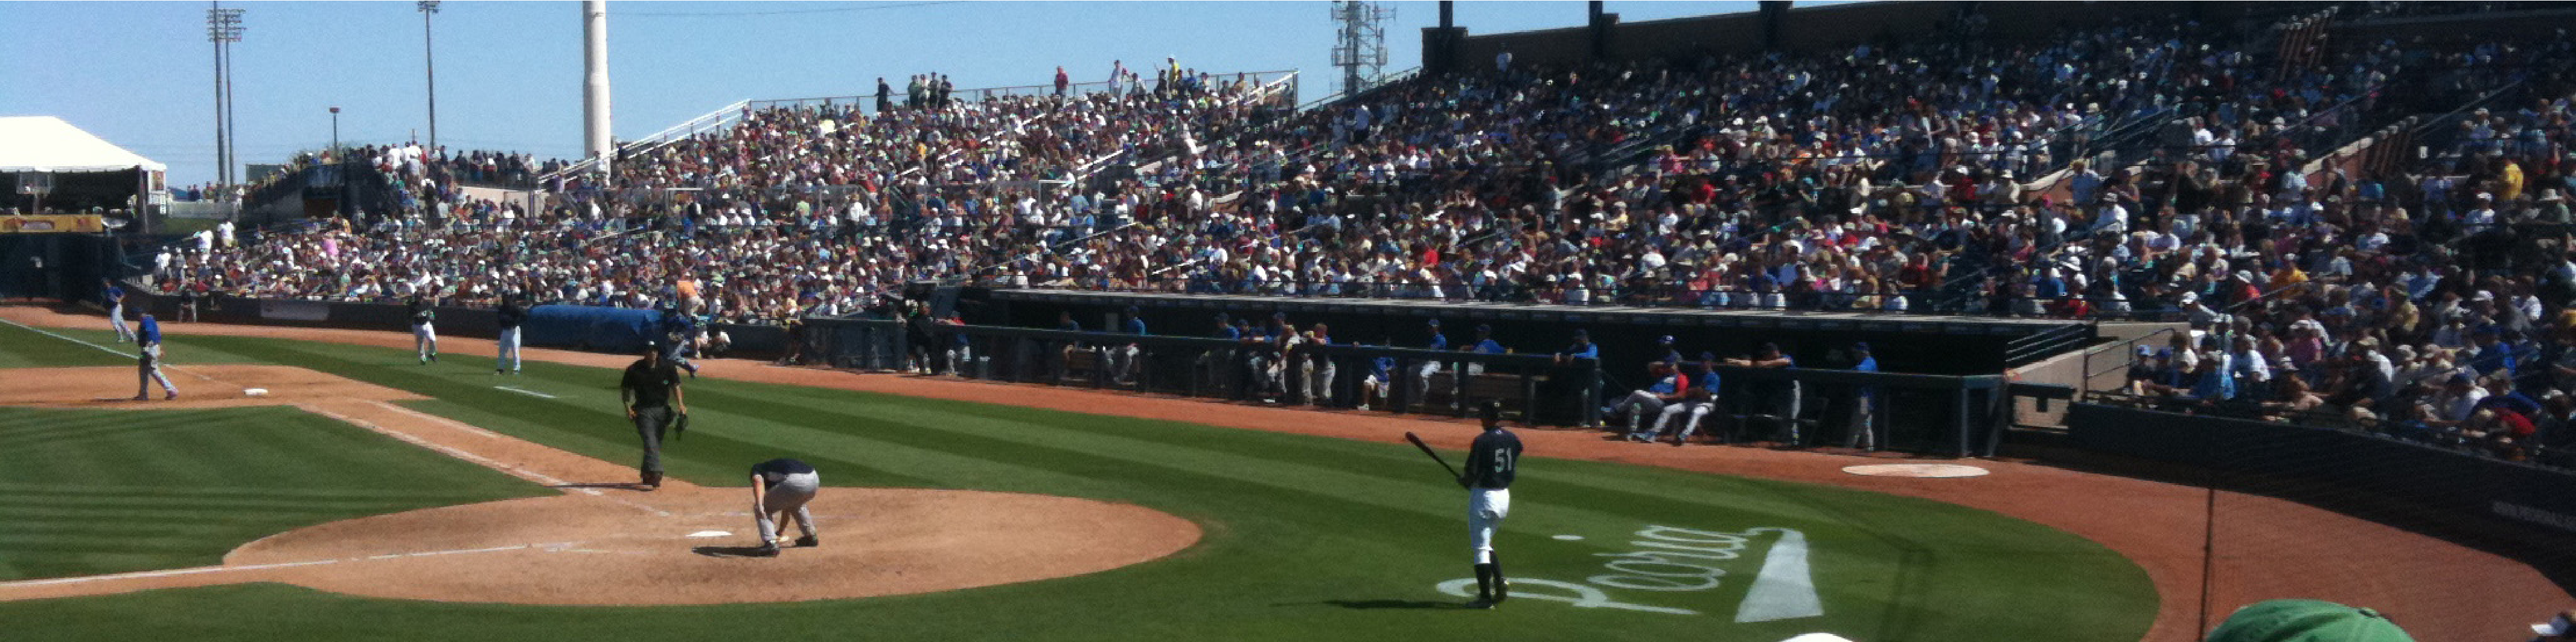
\includegraphics[width=\textwidth]{sampleteaser}
%   \caption{This is a teaser}
%   \label{fig:teaser}
% \end{teaserfigure}
% \end{verbatim}
%
%
% \DescribeMacro{\settopmatter}%
% Some information in the top matter is printed for certain journals
% or proceedings and suppressed for others.  You can override these
% defaults using the command \cs{settopmatter}\marg{settings}.  The
% settings and their meanings are listed in
% Table~\ref{tab:settopmatter}.  For example,
% \begin{verbatim}
% \settopmatter{printacmref=false, printccs=true, printfolios=true}
% \end{verbatim}
% The parameter |authorsperrow| requires some explanation.  In
% conference proceedings authors' information is typeset in boxes,
% several boxes per row (see |sample-sigconf.pdf|,
% |sample-sigplan.pdf|, etc.).  The number of boxes per row is
% determined automatically.  If you want to override this,
% you can do it using this parameter, for example,
% \begin{verbatim}
% \settopmatter{authorsperrow=4}
% \end{verbatim}
% However, in most cases you should \emph{not} do this and should use the
% default settings.  Setting |authorsperrow| to $0$ will revert it to the
% default settings.
%
% The parameter |printacmref| specifies whether to print the ACM
% bibliographic entry (default), or not.  Note that this entry is
% required for all articles over one page in length, and is optional
% for one-page articles (abstracts). 
%
% \begin{table}
%   \centering
%   \caption{Settings for the \cs{settopmatter} command}
%   \label{tab:settopmatter}
%   \begin{tabularx}{\textwidth}{llX}
%     \toprule
%     Parameter & Values & Meaning\\
%     \midrule
%     |printccs| & true/false & Whether to print CCS categories\\
%     |printacmref| & true/false & Whether to print the ACM bibliographic
%     entry\\
%     |printfolios| & true/false & Whether to print page numbers
%     (folios)\\
%     |authorsperrow| & numeric & Number of authors per row for the title
%     page in
%     conference proceedings formats\\
%     \bottomrule
%   \end{tabularx}
% \end{table}
%
%
% \DescribeMacro{\received}%
% The command \cs{received}\oarg{stage}\marg{date} sets the history of
% the publication.  The~\oarg{stage} argument is optional; the default
% is |Received| for the first date and |revised| for the subsequent
% ones.  For example,
% \begin{verbatim}
% \received{February 2007}
% \received[revised]{March 2009}
% \received[accepted]{June 2009}
% \end{verbatim}
%
%
% \DescribeMacro{\maketitle}%
% The macro \cs{maketitle} must be the last command in the top-matter
% group.  That is it must follow the commands defined in this section.
%
%
% \DescribeMacro{\shortauthors}%
% \emph{After} the command \cs{maketitle}, the macro \cs{shortauthors}
% stores the names of the authors for the running head.  You can
% redefine it if the list of author's name is too long, e.g.,
% \begin{verbatim}
% \maketitle
% \renewcommand{\shortauthors}{Zhou et al.}
% \end{verbatim}
%
%
%\subsection{Algorithms}
%\label{sec:ug_algorithms}
%
% There are now several good packages for typesetting
% algorithms~\cite{Fiorio15, Brito09, Heinz15}, and the authors are
% free to choose their favorite one.
%
%
%
%\subsection{Figures and tables}
%\label{sec:ug_floats}
%
% The new ACM styles use the standard \LaTeX\ interface for figures and
% tables.  There are some important items to be aware of, however.
%
% \begin{enumerate}
% \item The captions for figures must be entered \emph{after} the
% figure bodies and for tables \emph{before} the table bodies.
% \item The ACM uses the standard types for figures and tables and adds
% several new ones.  In total there are the following types:
% \begin{description}
% \item[figure, table:] a standard figure or table taking a full text
% width in one-column formats and one column width in two-column formats.
% \item[figure*, table*] in two-column formats, a special figure or
% table taking a full text width.
% \item[teaserfigure:] a special figure before \cs{maketitle}.
% \end{description}
%
% \item Accordingly, when scaling images, one should use the
% following sizes:
% \begin{enumerate}
% \item For |teaserfigure|, |figure| in one-column mode or |figure*| in
%   two-column mode, use \cs{textwidth}.  In one-column mode, you can also
%   use \cs{columnwidth}, which coincides with \cs{textwidth} in this
%   case.
% \item For |figure| in two-column mode, use \cs{columnwidth}.
% \end{enumerate}
%
% \end{enumerate}
%
% It is strongly recommended to use the package |booktabs|~\cite{Fear05}
% and follow its main principles of typography with respect to tables:
% \begin{enumerate}
% \item Never, ever use vertical rules.
% \item Never use double rules.
% \end{enumerate}
% It is also a good idea not to overuse horizontal rules.
%
% For table \emph{footnotes} you have several options described in the TeX
% FAQ~\cite{TeXFAQ}. The simplest one is to use a \cs{minipage}
% environment:
% \begin{verbatim}
% \begin{table}
% \caption{Simulation Configuration}
% \label{tab:conf}
% \begin{minipage}{\columnwidth}
% \begin{center}
% \begin{tabular}{ll}
%   \toprule
%   TERRAIN\footnote{This is a table footnote. This is a
%     table footnote. This is a table footnote.} &
%     (200\,m$\times$200\,m) Square\\
%   Node Number     & 289\\
%   Node Placement  & Uniform\\
%   Application     & Many-to-Many/Gossip CBR Streams\\
%   Payload Size    & 32 bytes\\
%   Routing Layer   & GF\\
%   MAC Layer       & CSMA/MMSN\\
%   Radio Layer     & RADIO-ACCNOISE\\
%   Radio Bandwidth & 250Kbps\\
%   Radio Range     & 20m--45m\\
%   \bottomrule
% \end{tabular}
% \end{center}
% \bigskip
% \footnotesize\emph{Source:} This is a table
%  sourcenote. This is a table sourcenote. This is a table
%  sourcenote.
%
%  \emph{Note:} This is a table footnote.
% \end{minipage}
% \end{table}
% \end{verbatim}
%
%
% Tables and figures are by default centered.  However, in some cases
% (for example, when you use several subimages per figure) you may
% need to override this.  A good way to do so is to put the contents
% into a \cs{minipage} of the width \cs{columnwidth}.
%
%
%\subsection{Descriptions of images}
%\label{sec:descriptions}
%
% \DescribeMacro{\Description}%
% Some readers of ACM publications might be visually challenged.
% These readers might use a voice-over software to read aloud the
% papers.  It is important to provide them a description of each
% image used in the paper.
%
% The command \cs{Description}\oarg{short description}\marg{long
% description} should be placed inside every \texttt{figure},
% \texttt{teaserfigure} or \texttt{marginfigure} environment to
% provide a description of the image(s) used in the figure.  Unlike
% \cs{caption}, which is used alongside the image, \cs{Description} is
% intended to be used instead of the image, for example,
% \begin{verbatim}
% \begin{figure}
%   \centering
%   \includegraphics{voltage}
%   \Description{A bell-like histogram centered at $0.5$~V with most
%   measurements between $0.2$~V and $0.8$~V}
%   \caption{Histogram of the measurements of voltage}
%   \label{fig:voltage}
% \end{figure}
% \end{verbatim}
% At present the lack of descriptions generates a warning at
% compilation.  
%
%\subsection{Theorems}
%\label{sec:ug_theorems}
%
% The ACM classes define two theorem styles and several pre-defined
% theorem environments:
% \begin{description}
% \item[acmplain:] this is the style used for
%   |theorem|,
%   |conjecture|,
%   |proposition|,
%   |lemma| and
%   |corollary|, and
% \item[acmdefinition:] this is the style used for
%   |example| and
%   |definition|.
% \end{description}
%
%
% These environments are defined by default.  In the unusual
% circumstance that a user does not wish to have these environments
% defined, the option |acmthm=false| in the preamble will suppress
% them.
%
%\subsection{Online-only and offline-only material}
%\label{sec:ug_screen}
%
% \DescribeEnv{printonly}%
% \DescribeEnv{screenonly}%
% Some supplementary material in ACM publications is put online but
% not in the printed version.  The text inside the environment
% |screenonly| will be typeset only when the option |screen| (see
% Section~\ref{sec:invocation}) is set to |true|.  Conversely, the
% text inside the environment |printonly| is typeset only when this
% option is set to |false|.  For example,
% \begin{verbatim}
% \section{Supplementary materials}
%
% \begin{printonly}
%   Supplementary materials are available in the online version of this paper.
% \end{printonly}
%
% \begin{screenonly}
%   (The actual supplementary materials.)
% \end{screenonly}
% \end{verbatim}
%
% We use the |comment| package for typesetting this code, so
% |\begin| and |\end| should start on a line of their own with
% no leading or trailing spaces.
%
%\subsection{Note about anonymous mode}
%\label{sec:ug_anonymous}
%
% \DescribeEnv{anonsuppress}%
% When the option |anonymous| is selected, \TeX\ suppresses author
% information (including the number of authors) for a blind review.
% However, sometimes the information identifying the authors may be
% present in the body of the paper.  For example,
% \begin{verbatim}
% \begin{anonsuppress}
%   This is the continuation of the previous work by the author
%   \cite{prev1, prev2}.
% \end{anonsuppress}
% \end{verbatim}
%
% As for the |printonly| and |screenonly| environments,
% |\begin{anonsuppress}| and |\end{anonsuppress}| should start on a
% line of their own with no leading or trailing spaces.
%
%\subsection{Acknowledgments}
%\label{sec:ug_acks}
%
% The traditional ``Acknowledgments'' section is conventionally used
% to thank persons and granting agencies for their help and support.
% However, there are several important considerations about this
% section.
%
% First, in anonymous mode this section must be omitted: it gives
% too much information to reviewers.  Second, data about
% grants is extracted and stored separately by the postprocessing
% software.  ACM classes provide facilities for both these tasks.
%
% \DescribeEnv{acks}%
% The environment |acks| starts an unnumbered section
% ``Acknowledgments'' unless the anonymous mode is chosen.  Put all
% thanks inside this environment.
%
% As for the |printonly| and |screenonly| environments,
% |\begin{acks}| and |\end{acks}| should start on a
% line of their own with no leading or trailing spaces.
%
% \DescribeMacro{\grantsponsor}%
% \DescribeMacro{\grantnum}%
% All financial support \emph{must} be listed using the commands
% \cs{grantsponsor} and \cs{grantnum}.  These commands tell the
% postprocessing software about the granting organization and
% grant.  The format of these commands is the following:
% \begin{quote}
%   \cs{grantsponsor}\marg{sponsorID}\marg{name}\marg{url}\\
%   \cs{grantnum}\oarg{url}\marg{sponsorID}\marg{number}.
% \end{quote}
% Here \marg{sponsorID} is the unique ID used to match grants to
% sponsors, \marg{name} is the name of the sponsor, \marg{url} is its
% URL, and \marg{number} is the grant number.  The \marg{sponsorID} of
% the \cs{grantnum} command must correspond to the \marg{sponsorID} of a
% \cs{grantsponsor} command.  Some awards have their own web pages,
% which you can include using the optional argument of the \cs{grantnum}
% command.
%
% At present \marg{sponsorID} is chosen by the authors and can be an
% arbitrary key in the same way the label of a \cs{cite} is arbitrarily
% chosen.  There might be a change to this policy if the ACM decides to
% create a global database of sponsoring organizations.
%
% Example:
% \begin{verbatim}
% \begin{acks}
%   The authors would like to thank Dr. Yuhua Li for providing the
%   matlab code of the \textit{BEPS} method.
%
%   The authors would also like to thank the anonymous referees for
%   their valuable comments and helpful suggestions. This work is
%   supported by the \grantsponsor{GS501100001809}{National Natural
%   Science Foundation of
%   China}{https://doi.org/10.13039/501100001809} under Grant
%   No.:~\grantnum{GS501100001809}{61273304}
%   and~\grantnum[http://www.nnsf.cn/youngscientists]{GS501100001809}{Young
%   Scientists' Support Program}.
% \end{acks}
% \end{verbatim}
%
%
%\subsection{Bibliography}
%\label{sec:ug_bibliography}
%
% The ACM uses the |natbib| package for formatting references and
% the Bib\TeX\ style file \path{ACM-Reference-Format.bst} for Bib\TeX\
% processing.  You can disable loading of |natbib| using the
% option |natbib=false| in \cs{documentclass}.  However, it is not
% recommended, as well as the use of Bib\TeX\ styles other than
% \path{ACM-Reference-Format.bst}, and may delay the processing of the
% manuscript.
%
%
% \DescribeMacro{\citestyle}%
% If you use |natbib|, you can select one of two predefined citation
% styles using the command \cs{citestyle}: the author-year format
% |acmauthoryear| or the numeric format |acmnumeric|.  For example,
% \begin{verbatim}
% \citestyle{acmauthoryear}
% \end{verbatim}
% Note that numeric citations are the default mode for most formats.
%
% \DescribeMacro{\setcitestyle}%
% You can further customize |natbib| using
% the \cs{setcitestyle} command, for example,
% \begin{verbatim}
% \setcitestyle{numbers,sort&compress}
% \end{verbatim}
%
% One of the more common versions is
% \begin{verbatim}
% \setcitestyle{nosort}
% \end{verbatim}
% It is useful if you do not like the way |natbib| sorts citation
% lists.
%
% If you use |natbib|, then commands like \cs{citep} and
% \cs{citeauthor} are automatically supported.  The command
% \cs{shortcite} is the same as \cs{cite} in numerical mode and cites
% the year in author-date mode.
%
% Note that before version~1.48 the command \cs{citeyear} put the year
% in parentheses.  In version~1.48 and later it produces just the
% year; the command \cs{citeyearpar} can be used to emulate its old
% behavior.
%
% There are several customized \BibTeX\ entry types and fields in the ACM
% style file \path{ACM-Reference-Format.bst} that you may want to be
% aware of.
%
% The style supports the fields \path{doi} and \path{url}, for example,
% \begin{verbatim}
%  doi =          "10.1145/1188913.1188915",
%  url =          "http://ccrma.stanford.edu/~jos/bayes/bayes.pdf",
% \end{verbatim}
%
% The style supports the arXiv-recommended fields \path{eprint} and
% (optionally) \path{primaryclass}, for example,
% \begin{verbatim}
%  eprint =       "960935712",
%  primaryclass = "cs",
% \end{verbatim}
% See the examples at \url{http://arxiv.org/hypertex/bibstyles/}.
%
% There are several  special entry types. Types \path{online} and
% \path{game} are used for Web pages and games, for example,
% \begin{verbatim}
% @online{Thornburg01,
%  author =       "Harry Thornburg",
%  year =         "2001",
%  title =        "Introduction to Bayesian Statistics",
%  url =          "http://ccrma.stanford.edu/~jos/bayes/bayes.html",
%  month =        mar,
%  lastaccessed = "March 2, 2005",
% }
% \end{verbatim}
% Entry types \path{artifactsoftware}, \path{artifactdataset} 
% (with synonyms \path{software} and \path{dataset}) can be used to
% cite software artifacts and datasets, for example,
% \begin{verbatim}
% @ArtifactSoftware{R,
%    title = {R: A Language and Environment for Statistical Computing},
%    author = {{R Core Team}},
%    organization = {R Foundation for Statistical Computing},
%    address = {Vienna, Austria},
%    year = {2019},
%    url = {https://www.R-project.org/},
%}
% @ArtifactDataset{UMassCitations,
%  author    =  {Sam Anzaroot and Andrew McCallum},
%  title     =  {{UMass} Citation Field Extraction Dataset},
%  year      = 2013,
%  url       =
%     {http://www.iesl.cs.umass.edu/data/data-umasscitationfield},
%  lastaccessed = {May 27, 2019}
% }
% \end{verbatim}
% 
%
% For these entry types you can use the \path{lastaccessed} field to add
% the access date for the URL.
% 
%
%
% There are two ways to enter video or audio sources in the
% bibliograpy corresponding to two different possibilies.  For
% standalone sources available online, you can use an \path{online}
% entry and set its \path{howpublished} field.  For example,
% \begin{verbatim}
% @online{Obama08,
%  author =       "Barack Obama",
%  year   =       "2008",
%  title  =       "A more perfect union",
%  howpublished = "Video",
%  day    =       "5",
%  url    =       "http://video.google.com/videoplay?docid=6528042696351994555",
%  month  =       mar,
%  lastaccessed = "March 21, 2008",
% }
% \end{verbatim}
%
% For sources available as attachments to conference proceedings
% and similar documents, you can use the usual \path{inproceedings}
% entry type and set its \path{howpublished} field:
% \begin{verbatim}
% @Inproceedings{Novak03,
%  author =       "Dave Novak",
%  title =        "Solder man",
%  booktitle =    "ACM SIGGRAPH 2003 Video Review on Animation theater Program",
%  year =         "2003",
%  publisher =    "ACM Press",
%  address =      "New York, NY",
%  pages =        "4",
%  month =        "March 21, 2008",
%  doi =          "10.9999/woot07-S422",
%  howpublished = "Video",
% }
% \end{verbatim}
%
% Sometimes you need to cite a complete issue of a journal.  The
% \path{periodical} entry type is intended for this:
% \begin{verbatim}
% @periodical{JCohen96,
%  key =          "Cohen",
%  editor =       "Jacques Cohen",
%  title =        "Special issue: Digital Libraries",
%  journal =      "Communications of the {ACM}",
%  volume =       "39",
%  number =       "11",
%  month =        nov,
%  year =         "1996",
% }
% \end{verbatim}
%
% If you do not know the year of publication, the style will add
% ``[n.\,d.]'' (for ``no date'') to the entry.
%
% If you do not know the author (this is often the case for online
% entries), use the |key| field to add a key for sorting and citations,
% for example,
% \begin{verbatim}
% @online{TUGInstmem,
%  key =          {TUG},
%  year  =        2017,
%  title =        "Institutional members of the {\TeX} Users Group",
%  url =          "http://wwtug.org/instmem.html",
%  lastaccessed = "May 27, 2017",
% }
% \end{verbatim}
%
% A note about sorting.  The current ACM bibliography styles always
% sort the entries according to authors names and publication year.
% There is a controversy about sorting names with ``von'' or ``van''
% part: should Ludwig van Beethoven be sorted under ``V'' or under
% ``B''?  The American practice is to use ``van'' in sorting, i.e. to
% file van Beethoven under ``V''.  However, some authorities recommend
% to sort Dutch persons according to their last names (see
% e.g. \url{https://www.ifla.org/files/assets/cataloguing/pubs/names-of-persons_1996.pdf}).
% While I do not want to take a part in this dispute, I would like to
% point to the old ``noopsort'' trick by Oren Patashnik.  Add to the
% \texttt{.bib} file the line
% \begin{verbatim}
% @PREAMBLE{"\providecommand{\noopsort}[1]{}"}
% \end{verbatim}
% and then encode the author as
% \begin{verbatim}
%  author = {Ludwig {\noopsort{Beethoven}}van Beethoven},
% \end{verbatim}
% This will make the author to be sorted as ``Beethoven'' rather than
% ``van Beethoven''.
%
%\subsection{Colors}
%\label{sec:ug_colors}
%
% While printed ACM publications are usually black and white, |screen|
% mode allows the use of colors.  The ACM classes pre-define several
% colors according to~\cite{ACMIdentityStandards}:  |ACMBlue|,
% |ACMYellow|, |ACMOrange|, |ACMRed|, |ACMLightBlue|, |ACMGreen|,
% |ACMPurple| and |ACMDarkBlue|.  You can use them in color
% assignments.
%
% The ACM provides the following recommendation on color use.
%
% The most accessible approach would be to ensure that your article is
% still readable when printed in greyscale. The most notable reasons
% for this are:
% \begin{enumerate}
% \item The most common type of inherited Color Vision Deficiency
% (CVD) is red-green (in which similar-brightness colors that differ
% only in their amounts of red or green are often confused), and it
% affects up to 8\% of males and 0.5\% of females of Northern European
% descent.
% \item The most common type of acquired Color Vision Deficiency (CVD)
% is blue-yellow (including mild cases for many older adults).
% \item Most printing is in black and white.
% \item Situational impairments (e.g., bright sunlight shining on a
% mobile screen) tend to reduce the entire color gamut, reducing color
% discriminability.
% \end{enumerate}
%
% \textbf{Note:} It is \emph{not} safe to encode information using
% only variations in color (i.e., only differences in hue and/or
% saturation) as there is bound to be someone affected!
%
% To ensure that you are using the most accessible colors, the ACM
% recommends that you choose sets of colors to help ensure suitable
% variations in when printed in greyscale by using either of the following tools:
% \begin{enumerate}
%  \item ColourBrewer: \url{http://colorbrewer2.org/}
%  \item ACE: The Accessible Colour Evaluator:
%    \url{http://daprlab.com/ace/} for designing WCAG 2.0 compliant
%    palettes.
%  \end{enumerate}
%
%
%\subsection{Other notable packages and typographic remarks}
%\label{sec:ug_other}
%
% Several other packages are recommended for specialized tasks.
%
% The package |subcaption|~\cite{Sommerfeldt13:Subcaption} is
% recommended for complex figures with several subplots or subfigures
% that require separate subcaptioning.  The packages
% |nomencl|~\cite{Nomencl} and
% |glossaries|~\cite{Talbot16:Glossaries} can be used for the
% automatic creation of the lists of symbols and concepts used.
%
%
% By default |acmart| prevents all widows and orphans (i.e., lonely
% lines at the beginning or end of the page) and hyphenation at
% the end of the page.  This is done by the rather strict settings
% \begin{verbatim}
% \widowpenalty=10000
% \clubpenalty=10000
% \brokenpenalty=10000
% \end{verbatim}
% However, this may lead to frustrating results when the authors must
% obey a page limit.  Setting these penalties to smaller values may
% help if you absolutely need to.
%
% Another problem might be the too strict line breaking rules.  Again,
% a strategically placed \cs{sloppy} command or putting the
% problematic paragraph inside \texttt{sloppypar} environment might
% help---but beware, the results might be, well, sloppy.
%
% Note that the uppercasing in section titles is done using
% the |textcase| package~\cite{Carlisle04:Textcase}, so the command
% \cs{NoCaseChange} inside the title may help to prevent extraneous
% uppercasing.
%
%
%
%\subsection{Disabled or forbidden commands}
%\label{sec:ug_disabled}
%
% The goal of |acmart| package is to provide a uniform look and feel
% for ACM publications.  Accordingly, a number of commands is
% forbidden or disabled in |acmart|.
%
% You may \emph{not} put several authors or several e-mails into a
% \cs{author} or \cs{email} command.  This may lead to errors or
% warning.
%
% You cannot change \cs{baselinestretch} in your document: this
% produces an error.
%
% You should not abuse the command \cs{vspace}:  this command may
% disturb the typesetting of ACM papers.
%
%\subsection{A note for wizards: \texttt{acmart-preload-hook.tex}}
%\label{sec:ug_preload}
%
% Sometimes you need to change the behavior of |acmart|.  The
% usual way to do this is to redefine commands in the preamble.
% However, these definitions are executed \emph{after} |acmart| is
% loaded and certain decisions are made.  This presents a number of
% problems.
%
% For example, one may want to use the |titletoc| package with |acmart|.
% This package should be loaded before |hyperref|.  However, since
% |acmart| loads |hyperref| itself, the line |\usepackage{titletoc}|
% in the preamble will lead to grief (see
% \url{http://tex.stackexchange.com/questions/357265/using-titletoc-with-acm-acmart-style}).
%
% Another example is passing options to a package.  Suppose you want to
% use the |dvipsnames| option of the |xcolor| package.  Normally you cannot do
% this because |acmart| loads this package itself without options.
%
% The file |acmart-preload-hook.tex| can be used to solve these
% problems.  If this file exists, it will be processed before any other
% package.  You can use this file to load packages or pass options to
% them.  For example, if you put in this file
% \begin{verbatim}
% \let\LoadClassOrig\LoadClass
% \renewcommand\LoadClass[2][]{\LoadClassOrig[#1]{#2}%
% \usepackage{titletoc}}
% \end{verbatim}
% then |titletoc| will be loaded before |hyperref|.  If you put in
% this file
% \begin{verbatim}
% \PassOptionsToPackage{dvipsnames}{xcolor}
% \end{verbatim}
% you will pass |dvipsnames| to |xcolor|.
%
% \textbf{Important note.}  This hook makes it too easy to create a
% manuscript that is not acceptable by the ACM.  It is even easier to
% create a file that cannot be compiled.  So please do not use it
% \emph{unless you know what you are doing.}  And if you use it,
% \emph{do not ask for support.}  If you decide to use this hook, you
% are on your own.
%
%
%\subsection{Currently supported publications}
%\label{sec:pubs}
%
%\bgroup\centering
% \begin{longtable}{>{\ttfamily}p{0.2\textwidth}@{}p{0.8\textwidth}}
%   \caption{ACM publications and arguments of the \cs{acmJournal}
%   command}
%   \label{tab:pubs}\\
%     \toprule
%     \normalfont Abbreviation & Publication \\
%     \midrule
% \endfirsthead
%   \caption[]{ACM publications and arguments of the \cs{acmJournal}
%   command (continued)}\\
%     \toprule
%     \normalfont Abbreviation & Publication \\
%     \midrule
% \endhead
% \bottomrule
% \endfoot
%     CIE & ACM Computers in Entertainment \\
%     CSUR & ACM Computing Surveys\\
%     DGOV & Digital Government: Research and Practice \\
%     DTRAP &  Digital Threats: Research and Practice\\
%     HEALTH & ACM Transactions on Computing for Healthcare\\
%     IMWUT & PACM on Interactive, Mobile, Wearable and Ubiquitous
%     Technologies\\
%     JACM &  Journal of the ACM \\
%     JDIQ & ACM Journal of Data and Information Quality \\
%     JEA & ACM Journal of Experimental Algorithmics \\
%     JERIC & ACM Journal of Educational Resources in Computing\\
%     JETC & ACM Journal on Emerging Technologies in Computing Systems \\
%     JOCCH & ACM Journal on Computing and Cultural Heritage \\
%     PACMCGIT & Proceedings of the ACM on Computer Graphics and
%     Interactive Techniques\\
%     PACMHCI & PACM on Human-Computer Interaction\\
%     PACMPL & PACM on Programming Languages \\
%     POMACS & PACM on Measurement and Analysis of Computing Systems \\
%     TAAS & ACM Transactions on Autonomous and Adaptive Systems\\
%     TACCESS & ACM Transactions on Accessible Computing\\
%     TACO & ACM Transactions on Architecture and Code Optimization \\
%     TALG & ACM Transactions on Algorithms \\
%     TALLIP & ACM Transactions on Asian and Low-Resource Language
%     Information Processing\\
%     TAP & ACM Transactions on Applied Perception \\
%     TCPS & ACM Transactions on Cyber-Physical Systems\\
%     TDS & ACM/IMS Transactions on Data Science\\
%     TEAC & ACM Transactions on Economics and Computation\\
%     TECS & ACM Transactions on Embedded Computing Systems \\
%     TELO & ACM Transactions on Evolutionary Learning \\
%     THRI & ACM Transactions on Human-Robot Interaction\\
%     TIIS & ACM Transactions on Interactive Intelligent Systems\\
%     TIOT & ACM Transactions on Internet of Things \\
%     TISSEC & ACM Transactions on Information and System Security\\
%     TIST & ACM Transactions on Intelligent Systems and Technology \\
%     TKDD & ACM Transactions on Knowledge Discovery from Data\\
%     TMIS & ACM Transactions on Management Information Systems\\
%     TOCE & ACM Transactions on Computing Education\\
%     TOCHI & ACM Transactions on Computer-Human Interaction\\
%     TOCL & ACM Transactions on Computational Logic\\
%     TOCS & ACM Transactions on Computer Systems \\
%     TOCT & ACM Transactions on Computation Theory \\
%     TODAES & ACM Transactions on Design Automation of Electronic Systems\\
%     TODS & ACM Transactions on Database Systems\\
%     TOG & ACM Transactions on Graphics\\
%     TOIS & ACM Transactions on Information Systems\\
%     TOIT & ACM Transactions on Internet Technology\\
%     TOMACS & ACM Transactions on Modeling and Computer Simulation \\
%     TOMM  & ACM Transactions on Multimedia Computing, Communications
%     and Applications \\
%     TOMPECS & ACM Transactions on Modeling and Performance Evaluation
%     of Computing Systems\\
%     TOMS & ACM Transactions on Mathematical Software\\
%     TOPC & ACM Transactions on Parallel Computing\\
%     TOPLAS & ACM Transactions on Programming Languages and Systems\\
%     TOPS & ACM Transactions on Privacy and Security\\
%     TOS & ACM Transactions on Storage\\
%     TOSEM & ACM Transactions on Software Engineering and Methodology\\
%     TOSN & ACM Transactions on Sensor Networks\\
%     TQC & ACM Transactions on Quantum Computing\\
%     TRETS & ACM Transactions on Reconfigurable Technology and Systems\\
%     TSAS & ACM Transactions on Spatial Algorithms and Systems\\
%     TSC & ACM Transactions on Social Computing\\
%     TSLP & ACM Transactions on Speech and Language Processing \\
%     TWEB & ACM Transactions on the Web\\
% \end{longtable}
%\egroup
%
% Besides the publications listed in Table~\ref{tab:pubs}, there is a
% special ``publication'' type FACMP, a forthcoming ACM publication,
% reserved for new journals which are not assigned an ISSN yet.  
%
%
%\subsection{A note about \texttt{sigchi-a} format}
%\label{sec:sigchi-a}
%
% Starting in Spring 2020 ACM retired SIGCHI Extended Abstract format
% (|sigchi-a|).  ACM will not, under any circumstances, accept
% documents in this format for publication and will not offer
% technical support to the authors who use this template.
%
% You may use this format in the |nonacm| mode only, as in
% \begin{verbatim}
% \documentclass[sigchi-a, nonacm]{acmart}
% \end{verbatim}
%
% 
%
% \DescribeEnv{sidebar}%
% \DescribeEnv{marginfigure}%
% \DescribeEnv{margintable}%
% This format has large margin uses for special figures and
% tables. This package provides three environments for this with
% optional captions:
% \begin{description}
% \item[sidebar:] textual information in the margin,
% \item[marginfigure:] a figure in the margin,
% \item[margintable:] a table in the margin.
% \end{description}
%
% The environments |figure| and |table| produce figures and tables
% with the width of the text column.  The environments |figure*| and
% |table*| produce ``wide'' figures and tables, which take a large
% part of the margin.  
%
% The horizontal sizes of figures are:
% \begin{enumerate}
% \item |figure|:  \cs{columnwidth},
% \item |marginfigure|: \cs{marginparwidth},
% \item |figure*|: \cs{fulltextwidth}.
% \end{enumerate}
% 
% 
%
% \StopEventually{
% \clearpage
% \bibliography{acmart}
% \bibliographystyle{unsrt}}
%
% \clearpage
%
%
%\section{Implementation}
%\label{sec:impl}
%
%\subsection{Identification}
%\label{sec:ident}
%
% We start with a declaration of who we are.  Most |.dtx| files put
% driver code in a separate~|.drv| driver file.  We roll this code into the
% main file and use the pseudo-guard |<gobble>| for it.
%    \begin{macrocode}
%<class>\NeedsTeXFormat{LaTeX2e}
%<*gobble>
\ProvidesFile{acmart.dtx}
%</gobble>
%<class>\ProvidesClass{acmart}
[2020/04/30 v1.71 Typesetting articles for the Association for Computing Machinery]
%    \end{macrocode}
%
% \changes{v1.00}{2016/04/14}{First released version}
% \changes{v1.01}{2016/04/18}{Defined ACM colors}
% \changes{v1.01}{2016/04/18}{Changed hyperref colors in screen mode
% (closes \url{https://github.com/borisveytsman/acmart/issues/1})}
% \changes{v1.01}{2016/04/18}{Set headheight to 1pc for all formats
% (closes \url{https://github.com/borisveytsman/acmart/issues/5})}
% \changes{v1.02}{2016/04/21}{Documentation changes
% (closes \url{https://github.com/borisveytsman/acmart/issues/13})}
% \changes{v1.02}{2016/04/21}{Added TOPS and TSC
% (closes \url{https://github.com/borisveytsman/acmart/issues/12})}
% \changes{v1.03}{2016/04/22}{Added authorversion option
% (closes \url{https://github.com/borisveytsman/acmart/issues/9})}
% \changes{v1.03}{2016/04/22}{Added anonsuppress environment}
% \changes{v1.04}{2016/04/26}{Updated bibliography for siggraph}
% \changes{v1.05}{2016/04/27}{Patched \cs{setcitestyle} command;
% closes \url{https://github.com/borisveytsman/acmart/issues/19}}
% \changes{v1.05}{2016/04/27}{Added processing doi numbers for
% acmsiggraph and doi numbers for sigproc.bib}
% \changes{v1.08}{2016/05/13}{SIGPLAN reformatting by Matthew Fluet}
% \changes{v1.08}{2016/05/13}{Typos corrected (Tobias Pape)}
% \changes{v1.09}{2016/05/18}{Revert SIGPLAN caption rules}
% \changes{v1.11}{2016/05/27}{Customization of ACM theorem styles and
% proof environment by Matthew Fluet}
% \changes{v1.12}{2016/05/30}{Documentation updates}
% \changes{v1.14}{2016/06/09}{\cs{citestyle} updates (Matthew Fluet)}
% \changes{v1.16}{2016/07/07}{Formatting header/footer (Matthew
% Fluet)}
% \changes{v1.18}{2016/07/10}{Natbib is now the default for all
% formats}
% \changes{v1.19}{2016/07/28}{Include 'Abstract', 'Acknowledgements',
% and 'References' in PDF bookmarks (Matthew Fluet)}
% \changes{v1.20}{2016/08/06}{Bug fixes for bst}
% \changes{v1.22}{2016/09/25}{More bibliography changes for Aptara}
% \changes{v1.23}{2016/11/04}{Add PACMPL journal option}
% \changes{v1.26}{2016/12/24}{Corrected \cs{shortcite} bug}
% \changes{v1.26}{2016/12/24}{Documentation typos fixed (thanks to
% Stephen Spencer)}
% \changes{v1.30}{2017/02/04}{Bibtex style now recognizes https:// in
% doi}
% \changes{v1.31}{2017/03/04}{Documentation changes}
% \changes{v1.32}{2017/03/07}{Format siggraph is now obsolete}
% \changes{v1.32}{2017/03/07}{Added POMACS journal option}
% \changes{v1.33}{2017/03/12}{BibTeX crossref bug corrected}
% \changes{v1.33}{2017/03/18}{BibTeX comma before articleno bug
% corrected}
% \changes{v1.33}{2017/03/18}{BibTeX numpages bug corrected}
% \changes{v1.33}{2017/03/28}{Added acmart-preload-hook}
% \changes{v1.33}{2017/03/33}{Documentation updates}
% \changes{v1.35}{2017/04/23}{BibTeX bug fixed: et al.}
% \changes{v1.36}{2017/05/12}{Added the possibility to adjust number of
% author boxes per row in conference formats}
% \changes{v1.37}{2017/05/13}{Set \cs{normalparindent}; Reduce list
% indentation (Matthew Fluet)}%
% \changes{v1.38}{2017/05/13}{Increase default font size for SIGPLAN}
% \changes{v1.40}{2017/05/27}{Bibliography changes}
% \changes{v1.40}{2017/06/15}{Added package cleveref}
% \changes{v1.40}{2017/06/16}{Added new copyright version:
% licensedcagov}
% \changes{v1.41}{2017/06/25}{Added new badges}
% \changes{v1.42}{2017/07/02}{Deleted ACM badges}
% \changes{v1.44}{2017/07/30}{Added package refcount}
% \changes{v1.44}{2017/07/30}{Deleted package cleveref}
% \changes{v1.44}{2017/07/30}{Put theorem defs in a separate style}
% \changes{v1.46}{2017/08/17}{Bst file bug fixes: label width is
% calculated correctly}
% \changes{v1.46}{2017/08/25}{Added etoolbox}
% \changes{v1.46}{2017/08/29}{Restore theorem defs to class file}
% \changes{v1.47}{2017/08/31}{New journal: THRI}
% \changes{v1.48}{2017/09/09}{Typos fixed (Jamie Davis)}
% \changes{v1.48}{2017/09/16}{Code prettying (Michael D.~Adams)}
% \changes{v1.48}{2017/09/23}{Misc entries in the bibliography no
% longer produce a separate date}
% \changes{v1.48}{2017/10/01}{Initial support for Biblatex (Daniel Thomas)}
% \changes{1.48}{2017/10/14}{Bib code cleanup (Zack Weinberg)}
% \changes{1.48}{2017/12/03}{Documentation update (siggraph)}
% \changes{1.49}{2018/01/24}{New journal:  DTRAP}
% \changes{1.53}{2018/04/14}{New journals: PACMCGIT, TIOT, TDSCI}
% \changes{1.53}{2018/04/14}{Rearranged docs}
% \changes{1.54}{2018/06/17}{Moved footnote stuff before hyperref call
% (Ross Moore)}
% \changes{1.56}{2018/11/11}{Documented \cs{Description}}
% \changes{1.57}{2018/12/16}{Booktabs package is now the default}
% \changes{1.58}{2019/02/09}{Changes in samples (Enrico Gregorio)}
% \changes{1.58}{2019/03/29}{New journal: HEALTH.  TDS is renamed to
% TDSCI} 
% \changes{1.60}{2019/04/22}{New option: urlbreakonhyphens}
% \changes{1.62}{2019/07/31}{New journal: TELO}
% \changes{1.63}{2019/08/04}{New journal: TQUANT}
% \changes{1.63}{2019/08/04}{New journal: FACMP} 
% \changes{1.63a}{2019/08/05}{Move: TQUANT to TQC}
% \changes{1.64}{2019/08/17}{Putting abstract after \cs{maketitle} now
% causes an error}
% \changes{1.65}{2019/10/19}{New journal: DGOV}
% \changes{1.66}{2019/12/18}{ACM reference format is now mandatory for
% papers over one page;  CCS concepts and keywords are now mandatory for
% papers over two pages}
% \changes{1.66}{2019/12/18}{Authors' addresses are mandatory for
% journal articles}
% \changes{1.71}{2020/05/01}{Retired sigchi and sigchi-a}
% \changes{1.71}{2020/05/02}{Bibliography change: volume for
% @inproceedings is now in brackets together with series}
% \changes{1.71}{2020/05/02}{LuaTeX now uses the OTF versions of fonts}
%
% And the driver code:
%    \begin{macrocode}
%<*gobble>
\documentclass{ltxdoc}
\usepackage{array,booktabs,amsmath,graphicx,fancyvrb,tabularx, longtable}
\usepackage[tt=false, type1=true]{libertine}
\usepackage[varqu]{zi4}
\usepackage[libertine]{newtxmath}
\usepackage[tableposition=top]{caption}
\usepackage{hypdoc}
\PageIndex
\CodelineIndex
\RecordChanges
\EnableCrossrefs
\begin{document}
  \DocInput{acmart.dtx}
\end{document}
%</gobble>
%<*class>
\def\@classname{acmart}
%    \end{macrocode}
%
%
%
%\subsection{Preload hook}
%\label{sec:preload}
%
% We preload |acmart-preload-hook|:
%    \begin{macrocode}
\InputIfFileExists{acmart-preload-hook.tex}{%
  \ClassWarning{\@classname}{%
    I am loading acmart-preload-hook.tex. You are fully responsible
    for any problems from now on.}}{}
%    \end{macrocode}
%
% \subsection{Options}
% \label{sec:options}
%
% We need |xkeyval| since some of our options may have values:
%    \begin{macrocode}
\RequirePackage{xkeyval}
%    \end{macrocode}
%
% We use |xstring| to check whether user input is valid
%    \begin{macrocode}
\RequirePackage{xstring}
%    \end{macrocode}
%
% We need |iftex| to check the engine
%    \begin{macrocode}
\RequirePackage{iftex}
%    \end{macrocode}
% 
% 
%
% \begin{macro}{format}
%   The possible formats
%    \begin{macrocode}
\define@choicekey*+{acmart.cls}{format}[\ACM@format\ACM@format@nr]{%
  manuscript, acmsmall, acmlarge, acmtog, sigconf, siggraph,
  sigplan, sigchi, sigchi-a}[manuscript]{}{%
  \ClassError{\@classname}{The option format must be manuscript,
    acmsmall, acmlarge, acmtog, sigconf, siggraph,
    sigplan, sigchi or sigchi-a}}
\def\@DeclareACMFormat#1{\DeclareOptionX{#1}{\setkeys{acmart.cls}{format=#1}}}
\@DeclareACMFormat{manuscript}
\@DeclareACMFormat{acmsmall}
\@DeclareACMFormat{acmlarge}
\@DeclareACMFormat{acmtog}
\@DeclareACMFormat{sigconf}
\@DeclareACMFormat{siggraph}
\@DeclareACMFormat{sigplan}
\@DeclareACMFormat{sigchi}
\@DeclareACMFormat{sigchi-a}
\ExecuteOptionsX{format}
%    \end{macrocode}
%
% \end{macro}
%
% \begin{macro}{\if@ACM@screen}
%   Whether we use screen mode
%    \begin{macrocode}
\define@boolkey+{acmart.cls}[@ACM@]{screen}[true]{%
  \if@ACM@screen
    \PackageInfo{\@classname}{Using screen mode}%
  \else
    \PackageInfo{\@classname}{Not using screen mode}%
  \fi}{\PackageError{\@classname}{The option screen can be either true or
    false}}
\ExecuteOptionsX{screen=false}
%    \end{macrocode}
%
% \end{macro}
%
% \begin{macro}{\if@ACM@urlbreakonhyphens}
% \changes{1.60}{2019/04/22}{introduced macro} 
%    \begin{macrocode}
\define@boolkey+{acmart.cls}[@ACM@]{urlbreakonhyphens}[true]{%
  \if@ACM@urlbreakonhyphens
    \PackageInfo{\@classname}{Using breaking urls on hyphens}%
  \else
    \PackageInfo{\@classname}{Not breaking urls on hyphens}%
  \fi}{\PackageError{\@classname}{The option urlbreakonhyphens can be either true or
    false}}
\ExecuteOptionsX{urlbreakonhyphens=true}
%    \end{macrocode}
% \end{macro}
%
% \begin{macro}{\if@ACM@acmthm}
% \changes{v1.44}{2017/07/30}{Added macro}
% \changes{v1.46}{2017/08/29}{Modified description}
%   Whether we define theorem-like environments.
%    \begin{macrocode}
\define@boolkey+{acmart.cls}[@ACM@]{acmthm}[true]{%
  \if@ACM@acmthm
    \PackageInfo{\@classname}{Requiring acmthm}%
  \else
    \PackageInfo{\@classname}{Suppressing acmthm}%
  \fi}{\PackageError{\@classname}{The option acmthm can be either true or
    false}}
\ExecuteOptionsX{acmthm=true}
%    \end{macrocode}
%
% \end{macro}
%
%
% \begin{macro}{\if@ACM@review}
% \changes{v1.48}{2017/09/09}{Review mode now switches on folios}
%   Whether we use review mode
%    \begin{macrocode}
\define@boolkey+{acmart.cls}[@ACM@]{review}[true]{%
  \if@ACM@review
    \PackageInfo{\@classname}{Using review mode}%
    \AtBeginDocument{\@ACM@printfoliostrue}%
  \else
    \PackageInfo{\@classname}{Not using review mode}%
  \fi}{\PackageError{\@classname}{The option review can be either true or
    false}}
\ExecuteOptionsX{review=false}
%    \end{macrocode}
%
% \end{macro}
%
% \begin{macro}{\if@ACM@authorversion}
% \changes{v1.03}{2016/04/22}{Added macro}
%   Whether we use author's-version mode
%    \begin{macrocode}
\define@boolkey+{acmart.cls}[@ACM@]{authorversion}[true]{%
  \if@ACM@authorversion
    \PackageInfo{\@classname}{Using authorversion mode}%
  \else
    \PackageInfo{\@classname}{Not using authorversion mode}%
  \fi}{\PackageError{\@classname}{The option authorversion can be either true or
    false}}
\ExecuteOptionsX{authorversion=false}
%    \end{macrocode}
%
% \end{macro}
%
% \begin{macro}{\if@ACM@nonacm}
% \changes{v1.54}{2018/05/08}{Added macro}
%   Special option for non-ACM publications
%   using the ACM typesetting options.
%    \begin{macrocode}
\define@boolkey+{acmart.cls}[@ACM@]{nonacm}[true]{%
  \if@ACM@nonacm
    \PackageInfo{\@classname}{Using nonacm mode}%
    \AtBeginDocument{\@ACM@printacmreffalse}%
    % in 'nonacm' mode we disable the "ACM Reference Format"
    % printing by default, but this can be re-enabled by the
    % user using \settopmatter{printacmref=true}
  \else
    \PackageInfo{\@classname}{Not using nonacm mode}%
  \fi}{\PackageError{\@classname}{The option nonacm can be either true or
    false}}
\ExecuteOptionsX{nonacm=false}
%    \end{macrocode}
%
% \end{macro}
%
% \begin{macro}{\if@ACM@balance}
% \changes{v1.57}{2018/12/16}{Added macro}
% Whether to balance the last page
%    \begin{macrocode}
\define@boolkey+{acmart.cls}[@ACM@]{balance}[true]{}{%
  \PackageError{\@classname}{The option balance can be either true or
    false}}
\ExecuteOptionsX{balance}
%    \end{macrocode}
% 
% \end{macro}
%
%
% \begin{macro}{\if@ACM@natbib@override}
% \changes{v1.12}{2016/05/30}{Added macro}
% \changes{v1.33}{2017/03/28}{Deleted macro}
% This macro is no longer used.
% \end{macro}
%
% \begin{macro}{\if@ACM@natbib}
%   Whether we use |natbib| mode
%    \begin{macrocode}
\define@boolkey+{acmart.cls}[@ACM@]{natbib}[true]{%
  \if@ACM@natbib
    \PackageInfo{\@classname}{Explicitly selecting natbib mode}%
  \else
    \PackageInfo{\@classname}{Explicitly deselecting natbib mode}%
  \fi}{\PackageError{\@classname}{The option natbib can be either true or
    false}}
\ExecuteOptionsX{natbib=true}
%    \end{macrocode}
%
% \end{macro}
%
%
% \begin{macro}{\if@ACM@anonymous}
%   Whether we use anonymous mode
%    \begin{macrocode}
\define@boolkey+{acmart.cls}[@ACM@]{anonymous}[true]{%
  \if@ACM@anonymous
    \PackageInfo{\@classname}{Using anonymous mode}%
  \else
    \PackageInfo{\@classname}{Not using anonymous mode}%
  \fi}{\PackageError{\@classname}{The option anonymous can be either true or
    false}}
\ExecuteOptionsX{anonymous=false}
%    \end{macrocode}
%
% \end{macro}
%
%
% \begin{macro}{\if@ACM@timestamp}
% \changes{v1.33}{2017/03/10}{Added macro (Michael D.~Adams)}
%   Whether we use timestamp mode
%    \begin{macrocode}
\define@boolkey+{acmart.cls}[@ACM@]{timestamp}[true]{%
  \if@ACM@timestamp
    \PackageInfo{\@classname}{Using timestamp mode}%
  \else
    \PackageInfo{\@classname}{Not using timestamp mode}%
  \fi}{\PackageError{\@classname}{The option timestamp can be either true or
    false}}
\ExecuteOptionsX{timestamp=false}
%    \end{macrocode}
%
% \end{macro}
%
%
% \begin{macro}{\if@ACM@authordraft}
% \changes{v1.33}{2017/03/28}{Added macro}
% \changes{v1.36}{2017/05/13}{Corrected typo, thanks to bargteil}
%   Whether we use author-draft mode
%    \begin{macrocode}
\define@boolkey+{acmart.cls}[@ACM@]{authordraft}[true]{%
  \if@ACM@authordraft
    \PackageInfo{\@classname}{Using authordraft mode}%
    \@ACM@timestamptrue
    \@ACM@reviewtrue
  \else
    \PackageInfo{\@classname}{Not using authordraft mode}%
  \fi}{\PackageError{\@classname}{The option authordraft can be either true or
    false}}
\ExecuteOptionsX{authordraft=false}
%    \end{macrocode}
%
% \end{macro}
%
%
% \begin{macro}{\ACM@fontsize}
%   The font size to pass to the base class
%    \begin{macrocode}
\def\ACM@fontsize{}
\DeclareOptionX{9pt}{\edef\ACM@fontsize{\CurrentOption}}
\DeclareOptionX{10pt}{\edef\ACM@fontsize{\CurrentOption}}
\DeclareOptionX{11pt}{\edef\ACM@fontsize{\CurrentOption}}
\DeclareOptionX{12pt}{\edef\ACM@fontsize{\CurrentOption}}
%    \end{macrocode}
%
% \end{macro}
%
%
% \changes{v1.01}{2016/04/18}{Explicitly put draft option
% (closes \url{https://github.com/borisveytsman/acmart/issues/4})}
%
%    \begin{macrocode}
\DeclareOptionX{draft}{\PassOptionsToClass{\CurrentOption}{amsart}}
\DeclareOptionX{*}{\PassOptionsToClass{\CurrentOption}{amsart}}
\ProcessOptionsX
\ClassInfo{\@classname}{Using format \ACM@format, number \ACM@format@nr}
%    \end{macrocode}
%
%
%
%\subsection{Setting switches}
%\label{sec:switches}
%
% \begin{macro}{\if@ACM@manuscript}
%   Whether we use manuscript mode
%    \begin{macrocode}
\newif\if@ACM@manuscript
%    \end{macrocode}
%
% \end{macro}
%
% \begin{macro}{\if@ACM@journal}
%   There are two kinds of publications: journals and books
%    \begin{macrocode}
\newif\if@ACM@journal
%    \end{macrocode}
%
% \end{macro}
%
%
% \begin{macro}{\if@ACM@journal@bibstrip}
% \changes{v1.59}{2019/04/20}{Introduced macro}
% Sometimes ACM wants a journal-like publication to have conference
% information in the bibstrip and vice versa, so we have an additional
% switch.
%    \begin{macrocode}
\newif\if@ACM@journal@bibstrip
%    \end{macrocode}
% 
% \end{macro}
%
% \begin{macro}{\if@ACM@sigchiamode}
%   The formatting of SIGCHI extended abstracts is quite unusual.  We have a
%   special switch for them.
%    \begin{macrocode}
\newif\if@ACM@sigchiamode
%    \end{macrocode}
%
% \end{macro}
%
%
% Setting up switches
%    \begin{macrocode}
\ifnum\ACM@format@nr=5\relax % siggraph
\ClassWarning{\@classname}{%
  The format siggraph is now obsolete.\MessageBreak
  I am switching to sigconf.}
  \setkeys{acmart.cls}{format=sigconf}
\fi
\ifnum\ACM@format@nr=7\relax % sigchi
\ClassWarning{\@classname}{%
  The format sigchi is now obsolete.\MessageBreak
  I am switching to sigconf.}
  \setkeys{acmart.cls}{format=sigconf}
\fi
\ifnum\ACM@format@nr=8\relax % sigchi
\ClassWarning{\@classname}{%
  ACM SIGCHI has retired the SIGCHI-A template\MessageBreak
  effective immediately. ACM is keeping this template\MessageBreak
  option available to authors who are working on legacy\MessageBreak
  documents only. ACM will not, under any circumstances,\MessageBreak
  accept documents in this format for publication and\MessageBreak
  will not offer technical support to the authors who use\MessageBreak
  this template.\MessageBreak
  ACM SIGCHI is directing Conference leaders and\MessageBreak
  authors to publish their articles using the SIGCONF\MessageBreak
  template call.}
\fi
\ifnum\ACM@format@nr=0\relax
  \@ACM@manuscripttrue
\else
  \@ACM@manuscriptfalse
\fi
\@ACM@sigchiamodefalse
\ifcase\ACM@format@nr
\relax % manuscript
  \@ACM@journaltrue
\or % acmsmall
  \@ACM@journaltrue
\or % acmlarge
  \@ACM@journaltrue
\or % acmtog
  \@ACM@journaltrue
\or % sigconf
  \@ACM@journalfalse
\or % siggraph
  \@ACM@journalfalse
 \or % sigplan
  \@ACM@journalfalse
 \or % sigchi
  \@ACM@journalfalse
\or % sigchi-a
  \@ACM@journalfalse
  \@ACM@sigchiamodetrue
\fi
\if@ACM@journal
 \@ACM@journal@bibstriptrue
\else
 \@ACM@journal@bibstripfalse
\fi
%    \end{macrocode}
%
%
%
%\subsection{Loading the base class and package}
%\label{sec:loading}
%
% \changes{v1.13}{2016/06/06}{Increased font size for ACM Large}
% \changes{v1.38}{2017/05/13}{Increase default font size for SIGPLAN}
%
%
% At this point we either have \cs{ACM@fontsize} or use defaults
%    \begin{macrocode}
\ifx\ACM@fontsize\@empty
  \ifcase\ACM@format@nr
  \relax % manuscript
    \def\ACM@fontsize{9pt}%
  \or % acmsmall
    \def\ACM@fontsize{10pt}%
  \or % acmlarge
    \def\ACM@fontsize{10pt}%
  \or % acmtog
    \def\ACM@fontsize{9pt}%
  \or % sigconf
    \def\ACM@fontsize{9pt}%
  \or % siggraph
    \def\ACM@fontsize{9pt}%
   \or % sigplan
    \def\ACM@fontsize{10pt}%
   \or % sigchi
    \def\ACM@fontsize{9pt}%
  \or % sigchi-a
    \def\ACM@fontsize{10pt}%
  \fi
\fi
\ClassInfo{\@classname}{Using fontsize \ACM@fontsize}
\LoadClass[\ACM@fontsize, reqno]{amsart}
\RequirePackage{microtype}
%    \end{macrocode}
%
%
% We need |etoolbox| for delayed code
%    \begin{macrocode}
\RequirePackage{etoolbox}
%    \end{macrocode}
%
% Booktabs is now the default
%    \begin{macrocode}
\RequirePackage{booktabs}
%    \end{macrocode}
% 
%
% We need |totpages| to calculate the number of pages and
% |refcount| to use that number
%    \begin{macrocode}
\RequirePackage{refcount}
\RequirePackage{totpages}
%    \end{macrocode}
%
% The \cs{collect@body} macro in |amsmath| is defined using \cs{def}.  We load
% |environ| to access the \cs{long} version of this command
%    \begin{macrocode}
\RequirePackage{environ}
%    \end{macrocode}
%
% We use |setspace| for double spacing
%    \begin{macrocode}
\if@ACM@manuscript
\RequirePackage{setspace}
\onehalfspacing
\fi
%    \end{macrocode}
%
% \changes{v1.40}{2017/06/05}{Added `textcase' package}
% We need |textcase| for better upcasing
%    \begin{macrocode}
\RequirePackage{textcase}
%    \end{macrocode}
%
%
%\subsection{Citations}
% \changes{v1.19}{2016/07/28}{Include 'References' in PDF bookmarks
% (Matthew Fluet)}
% \changes{v1.14}{2016/06/09}{Patched \cs{citestyle}}
% \changes{v1.55}{2016/08/012}{Typo corrected (Zack Weinberg)}
% We patch \cs{setcitestyle} to allow, for example,
% \cs{setcitestyle}|{sort}| and \cs{setcitestyle}|{nosort}|.  We patch
% \cs{citestyle} to warn about undefined citation styles.
%    \begin{macrocode}
\if@ACM@natbib
  \RequirePackage{natbib}
  \renewcommand{\bibsection}{%
     \section*{\refname}%
     \phantomsection\addcontentsline{toc}{section}{\refname}%
  }
  \renewcommand{\bibfont}{\bibliofont}
  \renewcommand\setcitestyle[1]{
  \@for\@tempa:=#1\do
  {\def\@tempb{round}\ifx\@tempa\@tempb
     \renewcommand\NAT@open{(}\renewcommand\NAT@close{)}\fi
   \def\@tempb{square}\ifx\@tempa\@tempb
     \renewcommand\NAT@open{[}\renewcommand\NAT@close{]}\fi
   \def\@tempb{angle}\ifx\@tempa\@tempb
     \renewcommand\NAT@open{$<$}\renewcommand\NAT@close{$>$}\fi
   \def\@tempb{curly}\ifx\@tempa\@tempb
     \renewcommand\NAT@open{\{}\renewcommand\NAT@close{\}}\fi
   \def\@tempb{semicolon}\ifx\@tempa\@tempb
     \renewcommand\NAT@sep{;}\fi
   \def\@tempb{colon}\ifx\@tempa\@tempb
     \renewcommand\NAT@sep{;}\fi
   \def\@tempb{comma}\ifx\@tempa\@tempb
     \renewcommand\NAT@sep{,}\fi
   \def\@tempb{authoryear}\ifx\@tempa\@tempb
     \NAT@numbersfalse\fi
   \def\@tempb{numbers}\ifx\@tempa\@tempb
     \NAT@numberstrue\NAT@superfalse\fi
   \def\@tempb{super}\ifx\@tempa\@tempb
     \NAT@numberstrue\NAT@supertrue\fi
   \def\@tempb{nobibstyle}\ifx\@tempa\@tempb
     \let\bibstyle=\@gobble\fi
   \def\@tempb{bibstyle}\ifx\@tempa\@tempb
     \let\bibstyle=\@citestyle\fi
   \def\@tempb{sort}\ifx\@tempa\@tempb
     \def\NAT@sort{\@ne}\fi
   \def\@tempb{nosort}\ifx\@tempa\@tempb
     \def\NAT@sort{\z@}\fi
   \def\@tempb{compress}\ifx\@tempa\@tempb
     \def\NAT@cmprs{\@ne}\fi
   \def\@tempb{nocompress}\ifx\@tempa\@tempb
     \def\NAT@cmprs{\z@}\fi
   \def\@tempb{sort&compress}\ifx\@tempa\@tempb
     \def\NAT@sort{\@ne}\def\NAT@cmprs{\@ne}\fi
   \def\@tempb{mcite}\ifx\@tempa\@tempb
     \let\NAT@merge\@ne\fi
   \def\@tempb{merge}\ifx\@tempa\@tempb
     \@ifnum{\NAT@merge<\tw@}{\let\NAT@merge\tw@}{}\fi
   \def\@tempb{elide}\ifx\@tempa\@tempb
     \@ifnum{\NAT@merge<\thr@@}{\let\NAT@merge\thr@@}{}\fi
   \def\@tempb{longnamesfirst}\ifx\@tempa\@tempb
     \NAT@longnamestrue\fi
   \def\@tempb{nonamebreak}\ifx\@tempa\@tempb
     \def\NAT@nmfmt#1{\mbox{\NAT@up#1}}\fi
   \expandafter\NAT@find@eq\@tempa=\relax\@nil
   \if\@tempc\relax\else
     \expandafter\NAT@rem@eq\@tempc
     \def\@tempb{open}\ifx\@tempa\@tempb
      \xdef\NAT@open{\@tempc}\fi
     \def\@tempb{close}\ifx\@tempa\@tempb
      \xdef\NAT@close{\@tempc}\fi
     \def\@tempb{aysep}\ifx\@tempa\@tempb
      \xdef\NAT@aysep{\@tempc}\fi
     \def\@tempb{yysep}\ifx\@tempa\@tempb
      \xdef\NAT@yrsep{\@tempc}\fi
     \def\@tempb{notesep}\ifx\@tempa\@tempb
      \xdef\NAT@cmt{\@tempc}\fi
     \def\@tempb{citesep}\ifx\@tempa\@tempb
      \xdef\NAT@sep{\@tempc}\fi
   \fi
  }%
  \NAT@@setcites
  }
  \renewcommand\citestyle[1]{%
    \ifcsname bibstyle@#1\endcsname%
    \csname bibstyle@#1\endcsname\let\bibstyle\@gobble%
    \else%
    \@latex@error{Undefined `#1' citestyle}%
    \fi
  }%
\fi
%    \end{macrocode}
%
% \begin{macro}{\bibstyle@acmauthoryear}
% \changes{v1.13}{2016/06/06}{Added macro}
% \changes{v1.14}{2016/06/09}{Moved def of \cs{bibstyle@acmauthoryear}
%   before use}
% \changes{v1.35}{2017/04/13}{Square brackets for author-year style}
%   The default author-year format:
%    \begin{macrocode}
\newcommand{\bibstyle@acmauthoryear}{%
  \setcitestyle{%
    authoryear,%
    open={[},close={]},citesep={;},%
    aysep={},yysep={,},%
    notesep={, }}}
%    \end{macrocode}
%
% \end{macro}
%
% \begin{macro}{\bibstyle@acmnumeric}
% \changes{v1.13}{2016/06/06}{Added macro}
% \changes{v1.14}{2016/06/09}{Moved def of \cs{bibstyle@numeric}
%   before use}
%   The default numeric format:
%    \begin{macrocode}
\newcommand{\bibstyle@acmnumeric}{%
  \setcitestyle{%
    numbers,sort&compress,%
    open={[},close={]},citesep={,},%
    notesep={, }}}
%    \end{macrocode}
%
% \end{macro}
%
% \changes{v1.28}{2017/01/07}{Corrected option natbib behavior}
% The default is numeric:
%    \begin{macrocode}
\if@ACM@natbib
\citestyle{acmnumeric}
\fi
%    \end{macrocode}
%
% \begin{macro}{\@startsection}
% \changes{v1.31}{2017/03/04}{Added \cs{tochangmeasure}}
% Before we call |hyperref|, we redefine \cs{startsection} commands to
% their \LaTeX\ defaults since the |amsart| ones are too AMS-specific.
% We need to do this early since we want |hyperref| to have a chance
% to redefine them again:
%    \begin{macrocode}
\def\@startsection#1#2#3#4#5#6{%
  \if@noskipsec \leavevmode \fi
  \par
  \@tempskipa #4\relax
  \@afterindenttrue
  \ifdim \@tempskipa <\z@
    \@tempskipa -\@tempskipa \@afterindentfalse
  \fi
  \if@nobreak
    \everypar{}%
  \else
    \addpenalty\@secpenalty\addvspace\@tempskipa
  \fi
  \@ifstar
    {\@ssect{#3}{#4}{#5}{#6}}%
    {\@dblarg{\@sect{#1}{#2}{#3}{#4}{#5}{#6}}}}
\def\@sect#1#2#3#4#5#6[#7]#8{%
  \edef\@toclevel{\ifnum#2=\@m 0\else\number#2\fi}%
  \ifnum #2>\c@secnumdepth
    \let\@svsec\@empty
  \else
    \refstepcounter{#1}%
    \protected@edef\@svsec{\@seccntformat{#1}\relax}%
  \fi
  \@tempskipa #5\relax
  \ifdim \@tempskipa>\z@
    \begingroup
      #6{%
        \@hangfrom{\hskip #3\relax\@svsec}%
          \interlinepenalty \@M #8\@@par}%
    \endgroup
    \csname #1mark\endcsname{#7}%
    \ifnum #2>\c@secnumdepth \else
        \@tochangmeasure{\csname the#1\endcsname}%
    \fi
    \addcontentsline{toc}{#1}{%
      \ifnum #2>\c@secnumdepth \else
        \protect\numberline{\csname the#1\endcsname}%
      \fi
      #7}%
  \else
    \def\@svsechd{%
      #6{\hskip #3\relax
      \@svsec #8}%
      \csname #1mark\endcsname{#7}%
      \ifnum #2>\c@secnumdepth \else
        \@tochangmeasure{\csname the#1\endcsname\space}%
      \fi
      \addcontentsline{toc}{#1}{%
        \ifnum #2>\c@secnumdepth \else
          \protect\numberline{\csname the#1\endcsname}%
        \fi
        #7}}%
  \fi
  \@xsect{#5}}
\def\@xsect#1{%
  \@tempskipa #1\relax
  \ifdim \@tempskipa>\z@
    \par \nobreak
    \vskip \@tempskipa
    \@afterheading
  \else
    \@nobreakfalse
    \global\@noskipsectrue
    \everypar{%
      \if@noskipsec
        \global\@noskipsecfalse
       {\setbox\z@\lastbox}%
        \clubpenalty\@M
        \begingroup \@svsechd \endgroup
        \unskip
        \@tempskipa #1\relax
        \hskip -\@tempskipa
      \else
        \clubpenalty \@clubpenalty
        \everypar{}%
      \fi}%
  \fi
  \ignorespaces}
\def\@seccntformat#1{\csname the#1\endcsname\quad}
\def\@ssect#1#2#3#4#5{%
  \@tempskipa #3\relax
  \ifdim \@tempskipa>\z@
    \begingroup
      #4{%
        \@hangfrom{\hskip #1}%
          \interlinepenalty \@M #5\@@par}%
    \endgroup
  \else
    \def\@svsechd{#4{\hskip #1\relax #5}}%
  \fi
  \@xsect{#3}}
%    \end{macrocode}
%
% \end{macro}
%
% \begin{macro}{\@startsection}
% \changes{v1.31}{2017/03/04}{Rededined macro}
% \changes{v1.43}{2017/07/09}{Added \cs{makeatletter}}
%   The |amsart| package redefines \cs{startsection}.  Here we redefine
%   it again to make the table of contents work.
%    \begin{macrocode}
\def\@starttoc#1#2{\begingroup\makeatletter
  \setTrue{#1}%
  \par\removelastskip\vskip\z@skip
  \@startsection{section}\@M\z@{\linespacing\@plus\linespacing}%
    {.5\linespacing}{\centering\contentsnamefont}{#2}%
  \@input{\jobname.#1}%
  \if@filesw
    \@xp\newwrite\csname tf@#1\endcsname
    \immediate\@xp\openout\csname tf@#1\endcsname \jobname.#1\relax
  \fi
  \global\@nobreakfalse \endgroup
  \addvspace{32\p@\@plus14\p@}%
}
%    \end{macrocode}
%
% \end{macro}
%
% \begin{macro}{\l@subsection}
% \changes{v1.40}{2017/05/27}{Redefined macro}
%   Section spacing is more generous than for |amsart|
%    \begin{macrocode}
\def\l@section{\@tocline{1}{0pt}{1pc}{2pc}{}}
%    \end{macrocode}
% \end{macro}
%
% \begin{macro}{\l@subsection}
% \changes{v1.31}{2017/03/04}{Redefined macro}
%   The spacing in |amsart| is too large
%    \begin{macrocode}
\def\l@subsection{\@tocline{2}{0pt}{1pc}{3pc}{}}
%    \end{macrocode}
%
% \end{macro}
% \begin{macro}{\l@subsubsection}
% \changes{v1.31}{2017/03/04}{Redefined macro}
% \changes{v1.71}{2020/04/30}{Bug fixed (thanks to Andrew Black)}
%   The spacing in |amsart| is too large
%    \begin{macrocode}
\def\l@subsubsection{\@tocline{3}{0pt}{1pc}{5pc}{}}
%    \end{macrocode}
%
% \end{macro}
%
% We need to define foonote-related stuff before the call to hyperref
% (Ross Moore)
% \begin{macro}{\@makefntext}
%   We do not use indentation for footnotes
%    \begin{macrocode}
\def\@makefntext{\noindent\@makefnmark}
%    \end{macrocode}
%
% \end{macro}
%
% \begin{macro}{\@footnotetext}
%   In |sigchi-a| mode our footnotes are in the margin!
%    \begin{macrocode}
\if@ACM@sigchiamode
\long\def\@footnotetext#1{\marginpar{%
    \reset@font\small
    \interlinepenalty\interfootnotelinepenalty
    \protected@edef\@currentlabel{%
       \csname p@footnote\endcsname\@thefnmark
    }%
    \color@begingroup
      \@makefntext{%
        \rule\z@\footnotesep\ignorespaces#1\@finalstrut\strutbox}%
    \color@endgroup}}%
\fi
%    \end{macrocode}
%
% \end{macro}
%
% \begin{macro}{\@mpfootnotetext}
% \changes{v1.13}{2016/06/06}{Made minipage footnotes centered}
%   We want the footnotes in minipages centered:
%    \begin{macrocode}
\long\def\@mpfootnotetext#1{%
  \global\setbox\@mpfootins\vbox{%
    \unvbox\@mpfootins
    \reset@font\footnotesize
    \hsize\columnwidth
    \@parboxrestore
    \protected@edef\@currentlabel
         {\csname p@mpfootnote\endcsname\@thefnmark}%
    \color@begingroup\centering
      \@makefntext{%
        \rule\z@\footnotesep\ignorespaces#1\@finalstrut\strutbox}%
    \color@endgroup}}
%    \end{macrocode}
%
% \end{macro}
%
% \begin{macro}{\@makefnmark}
% \changes{v1.17}{2016/067/09}{Redefined}
%   AMS classes use a buggy definition of \cs{makefnmark}.  We revert
%   to the standard one.
%    \begin{macrocode}
\def\@makefnmark{\hbox{\@textsuperscript{\normalfont\@thefnmark}}}
%    \end{macrocode}
%
% \end{macro}
%
%
% And now, |hyperref|
% \changes{v1.28}{2017/01/07}{Got rid of warnings in pdf keywords}
% \changes{v1.46}{2017/08/25}{Delayed hypersetup since journal options
% may change screen mode}
% \changes{v1.55}{2018/10/20}{Now we use purple color for links}
% \changes{v1.58}{2019/26/01}{Suppressed \cs{addtocounter} in pdf subject}
%    \begin{macrocode}
\let\@footnotemark@nolink\@footnotemark
\let\@footnotetext@nolink\@footnotetext
\RequirePackage[bookmarksnumbered,unicode]{hyperref}
\pdfstringdefDisableCommands{%
  \def\addtocounter#1#2{}%
  \def\unskip{}%
  \def\textbullet{- }%
  \def\textrightarrow{ -> }%
  \def\footnotemark{}%
}
\urlstyle{rm}
\ifcase\ACM@format@nr
\relax % manuscript
\or % acmsmall
\or % acmlarge
\or % acmtog
\or % sigconf
\or % siggraph
\or % sigplan
  \urlstyle{sf}
\or % sigchi
\or % sigchi-a
  \urlstyle{sf}
\fi
\AtEndPreamble{%
  \if@ACM@urlbreakonhyphens
    \def\do@url@hyp{\do\-}%
  \fi
  \if@ACM@screen
    \hypersetup{colorlinks,
      linkcolor=ACMPurple,
      citecolor=ACMPurple,
      urlcolor=ACMDarkBlue,
      filecolor=ACMDarkBlue}
    \else
    \hypersetup{hidelinks}
  \fi
  \hypersetup{pdflang={en},
    pdfdisplaydoctitle}}
%    \end{macrocode}
%
% Bibliography mangling.
% \changes{v1.33}{2017/03/23}{Moved \cs{citename} definition for
% non-natbib bibliography, so a package may redefine it}
% \changes{v1.48}{2017/09/23}{\cs{citeyear} no longer behaves like
% \cs{citeyearpar}}
%    \begin{macrocode}
\if@ACM@natbib
  \let\citeN\cite
  \let\cite\citep
  \let\citeANP\citeauthor
  \let\citeNN\citeyearpar
  \let\citeyearNP\citeyear
  \let\citeNP\citealt
  \DeclareRobustCommand\citeA
     {\begingroup\NAT@swafalse
       \let\NAT@ctype\@ne\NAT@partrue\NAT@fullfalse\NAT@open\NAT@citetp}%
  \providecommand\newblock{}%
\else
  \AtBeginDocument{%
    \let\shortcite\cite%
    \providecommand\citename[1]{#1}}
\fi
\newcommand\shortcite[2][]{%
  \ifNAT@numbers\cite[#1]{#2}\else\citeyearpar[#1]{#2}\fi}
%    \end{macrocode}
%
%
% \begin{macro}{\bibliographystyle}
% \changes{v1.13}{2016/06/06}{Redefined macro}
%   The |amsart| package redefines \cs{bibliographystyle} since it
%   prefers the AMS bibliography style.  We turn it back to the
%   \LaTeX\ definition:
%    \begin{macrocode}
\def\bibliographystyle#1{%
  \ifx\@begindocumenthook\@undefined\else
    \expandafter\AtBeginDocument
  \fi
    {\if@filesw
       \immediate\write\@auxout{\string\bibstyle{#1}}%
     \fi}}
%    \end{macrocode}
%
% \end{macro}
%
%
% Graphics and color.
% \changes{1.48}{2017/10/22}{Added prologue option to xcolor}
%    \begin{macrocode}
\RequirePackage{graphicx}
\RequirePackage[prologue]{xcolor}
%    \end{macrocode}
%
% We define ACM colors according to~\cite{ACMIdentityStandards}:
%    \begin{macrocode}
\definecolor[named]{ACMBlue}{cmyk}{1,0.1,0,0.1}
\definecolor[named]{ACMYellow}{cmyk}{0,0.16,1,0}
\definecolor[named]{ACMOrange}{cmyk}{0,0.42,1,0.01}
\definecolor[named]{ACMRed}{cmyk}{0,0.90,0.86,0}
\definecolor[named]{ACMLightBlue}{cmyk}{0.49,0.01,0,0}
\definecolor[named]{ACMGreen}{cmyk}{0.20,0,1,0.19}
\definecolor[named]{ACMPurple}{cmyk}{0.55,1,0,0.15}
\definecolor[named]{ACMDarkBlue}{cmyk}{1,0.58,0,0.21}
%    \end{macrocode}
%
%
% Author-draft mode or sigchi-a mode
%    \begin{macrocode}
\if@ACM@authordraft
  \RequirePackage{draftwatermark}
  \SetWatermarkFontSize{0.5in}
  \SetWatermarkColor[gray]{.9}
  \SetWatermarkText{\parbox{12em}{\centering
      Unpublished working draft.\\
      Not for distribution.}}
\else
  \if@ACM@sigchiamode
    \if@ACM@nonacm\else
      \RequirePackage{draftwatermark}
      \SetWatermarkFontSize{0.5in}
      \SetWatermarkColor[gray]{.9}
      \SetWatermarkText{\parbox{12em}{\centering
          Legacy document. \\
          Not for publication in an ACM venue}}
    \fi
  \fi  
\fi
%    \end{macrocode}
%
%
%\subsection{Paper size and paragraphing}
%\label{sec:paper}
%
% \changes{v1.17}{2016/07/07}{Slightly decreased margins for sigs}
% \changes{v1.29}{2017/01/22}{Increased head to 13pt}
% \changes{v1.40}{2017/07/15}{Added heightrounded to geometry}
% \changes{v1.56}{2018/10/16}{Make two-column layouts flush (Philip Quinn)}
% We use |geometry| for dimensions.  Note that the present margins do not
% depend on the font size option---we might need to change this.
% See \url{https://github.com/borisveytsman/acmart/issues/5#issuecomment-272881329}.
%    \begin{macrocode}
\RequirePackage{geometry}
\ifcase\ACM@format@nr
\relax % manuscript
   \geometry{letterpaper,head=13pt,
   marginparwidth=6pc,heightrounded}%
\or % acmsmall
   \geometry{twoside=true,
     includeheadfoot, head=13pt, foot=2pc,
     paperwidth=6.75in, paperheight=10in,
     top=58pt, bottom=44pt, inner=46pt, outer=46pt,
     marginparwidth=2pc,heightrounded
   }%
\or % acmlarge
   \geometry{twoside=true, head=13pt, foot=2pc,
     paperwidth=8.5in, paperheight=11in,
     includeheadfoot,
     top=78pt, bottom=114pt, inner=81pt, outer=81pt,
     marginparwidth=4pc,heightrounded
     }%
\or % acmtog
   \geometry{twoside=true, head=13pt, foot=2pc,
     paperwidth=8.5in, paperheight=11in,
     includeheadfoot, columnsep=24pt,
     top=52pt, bottom=75pt, inner=52pt, outer=52pt,
     marginparwidth=2pc,heightrounded
     }%
\or % sigconf
   \geometry{twoside=true, head=13pt,
     paperwidth=8.5in, paperheight=11in,
     includeheadfoot, columnsep=2pc,
     top=57pt, bottom=73pt, inner=54pt, outer=54pt,
     marginparwidth=2pc,heightrounded
     }%
\or % siggraph
   \geometry{twoside=true, head=13pt,
     paperwidth=8.5in, paperheight=11in,
     includeheadfoot, columnsep=2pc,
     top=57pt, bottom=73pt, inner=54pt, outer=54pt,
     marginparwidth=2pc,heightrounded
     }%
\or % sigplan
   \geometry{twoside=true, head=13pt,
     paperwidth=8.5in, paperheight=11in,
     includeheadfoot=false, columnsep=2pc,
     top=1in, bottom=1in, inner=0.75in, outer=0.75in,
     marginparwidth=2pc,heightrounded
     }%
\or % sigchi
   \geometry{twoside=true, head=13pt,
     paperwidth=8.5in, paperheight=11in,
     includeheadfoot, columnsep=2pc,
     top=66pt, bottom=73pt, inner=54pt, outer=54pt,
     marginparwidth=2pc,heightrounded
     }%
\or % sigchi-a
   \geometry{twoside=false, head=13pt,
     paperwidth=11in, paperheight=8.5in,
     includeheadfoot, marginparsep=72pt,
     marginparwidth=170pt, columnsep=20pt,
     top=72pt, bottom=72pt, left=314pt, right=72pt
     }%
     \@mparswitchfalse
     \reversemarginpar
\fi
%    \end{macrocode}
%
%
% \begin{macro}{\parindent}
% \begin{macro}{\parskip}
%   Paragraphing
%    \begin{macrocode}
\setlength\parindent{10\p@}
\setlength\parskip{\z@}
\ifcase\ACM@format@nr
\relax % manuscript
\or % acmsmall
\or % acmlarge
\or % acmtog
  \setlength\parindent{9\p@}%
\or % sigconf
\or % siggraph
\or % sigplan
\or % sigchi
\or % sigchi-a
\fi
%    \end{macrocode}
%
% \end{macro}
% \end{macro}
%
% \begin{macro}{\normalparindent}
% \changes{v1.37}{2017/05/13}{Set \cs{normalparindent} (Matthew Fluet)}%
%   The |amsart| package defines the \cs{normalparindent} length and
%   initializes it to 12pt (the value of \cs{parindent} in |amsart|).  It
%   is later used to set the \cs{listparindent} length in the |quotation|
%   environment and the \cs{parindent} length in the \cs{@footnotetext}
%   command.  We set \cs{normalparindent} to the value of \cs{parindent}
%   as selected by |acmart| for consistent paragraph indents.
%    \begin{macrocode}
\setlength\normalparindent{\parindent}
%    \end{macrocode}
%
% \end{macro}
%
% Footnotes require some consideration.  We have several layers of
% footnotes:  frontmatter footnotes, ``regular'' footnotes and the
% special insert for the bibstrip.  In the old ACM classes, the bibstrip
% was a \cs{@float}.  The problem with floats is that they tend to, well,
% float---and we want the guarantee they stay.
%
% We use |manyfoot| for layered footnotes instead.
%
% \begin{macro}{\copyrightpermissionfootnoterule}
% \changes{v1.12}{2016/05/30}{Added macro}
%   This is the footnote rule that separates the bibstrip from the rest of
%   the paper.  It is a full width rule.
%    \begin{macrocode}
\def\copyrightpermissionfootnoterule{\kern-3\p@
  \hrule \@width \columnwidth \kern 2.6\p@}
%    \end{macrocode}
% \end{macro}
%
%    \begin{macrocode}
\RequirePackage{manyfoot}
\SelectFootnoteRule[2]{copyrightpermission}
\DeclareNewFootnote{authorsaddresses}
\SelectFootnoteRule[2]{copyrightpermission}
\DeclareNewFootnote{copyrightpermission}
%    \end{macrocode}
%
%
% \begin{macro}{\footnoterule}
% \changes{v1.12}{2016/05/30}{Made shorter}
%   Tschichold's rules:
%    \begin{macrocode}
\def\footnoterule{\kern-3\p@
  \hrule \@width 4pc \kern 2.6\p@}
%    \end{macrocode}
%
% \end{macro}
%
% \begin{macro}{\endminipage}
%   We do not use footnote rules in minipages
%    \begin{macrocode}
\def\endminipage{%
    \par
    \unskip
    \ifvoid\@mpfootins\else
      \vskip\skip\@mpfootins
      \normalcolor
      \unvbox\@mpfootins
    \fi
    \@minipagefalse
  \color@endgroup
  \egroup
  \expandafter\@iiiparbox\@mpargs{\unvbox\@tempboxa}}
%    \end{macrocode}
%
% \end{macro}
%
%
% \begin{macro}{\@textbottom}
% \changes{v1.31}{2017/03/04}{Redefined}
%   Add some stretch according to David Carlisle's advice at
%   \url{http://tex.stackexchange.com/a/62318/5522}
%    \begin{macrocode}
\def\@textbottom{\vskip \z@ \@plus 1pt}
\let\@texttop\relax
%    \end{macrocode}
%
% \end{macro}
%
% In two-column layouts, force both columns to be the same height by inserting
% extra internal vertical space to fill out the page.
%    \begin{macrocode}
\ifcase\ACM@format@nr
\relax % manuscript
\or % acmsmall
\or % acmlarge
\or % acmtog
  \flushbottom
\or % sigconf
  \flushbottom
\or % siggraph
  \flushbottom
\or % sigplan
  \flushbottom
\or % sigchi
  \flushbottom
\or % sigchi-a
\fi
%    \end{macrocode}
%
%\subsection{Fonts}
%\label{sec:fonts}
%
% \changes{v1.12}{2016/05/30}{Added graceful behavior when libertine
% fonts are absent}
% \changes{v1.33}{2017/03/29}{Added cmap and glyphtounicode}
% \changes{v1.40}{2017/05/27}{Added Ross Moore code for glyphtounicode}
%
% Somehow PDFTeX and XeTeX require different incantations to make a PDF
% compliant with the current Acrobat bugs.  Xpdf is much better.
%
% The code below is by Ross Moore.
%    \begin{macrocode}
\RequirePackage{iftex}
\ifPDFTeX
% lcdf-typetools glyphtounicode.tex, Version 2.95
% Contents: Glyph mapping information for pdftex, used for PDF searching
% Generated from:
% - glyphlist.txt, Version 2.0
% - texglyphlist.txt, Version 2.95
% - texglyphlist-g2u.txt, Version 2.95
\pdfglyphtounicode{A}{0041}
\pdfglyphtounicode{AE}{00C6}
\pdfglyphtounicode{AEacute}{01FC}
\pdfglyphtounicode{AEmacron}{01E2}
\pdfglyphtounicode{AEsmall}{00E6}
\pdfglyphtounicode{Aacute}{00C1}
\pdfglyphtounicode{Aacutesmall}{00E1}
\pdfglyphtounicode{Abreve}{0102}
\pdfglyphtounicode{Abreveacute}{1EAE}
\pdfglyphtounicode{Abrevecyrillic}{04D0}
\pdfglyphtounicode{Abrevedotbelow}{1EB6}
\pdfglyphtounicode{Abrevegrave}{1EB0}
\pdfglyphtounicode{Abrevehookabove}{1EB2}
\pdfglyphtounicode{Abrevetilde}{1EB4}
\pdfglyphtounicode{Acaron}{01CD}
\pdfglyphtounicode{Acircle}{24B6}
\pdfglyphtounicode{Acircumflex}{00C2}
\pdfglyphtounicode{Acircumflexacute}{1EA4}
\pdfglyphtounicode{Acircumflexdotbelow}{1EAC}
\pdfglyphtounicode{Acircumflexgrave}{1EA6}
\pdfglyphtounicode{Acircumflexhookabove}{1EA8}
\pdfglyphtounicode{Acircumflexsmall}{00E2}
\pdfglyphtounicode{Acircumflextilde}{1EAA}
\pdfglyphtounicode{Acute}{00B4}
\pdfglyphtounicode{Acutesmall}{00B4}
\pdfglyphtounicode{Acyrillic}{0410}
\pdfglyphtounicode{Adblgrave}{0200}
\pdfglyphtounicode{Adieresis}{00C4}
\pdfglyphtounicode{Adieresiscyrillic}{04D2}
\pdfglyphtounicode{Adieresismacron}{01DE}
\pdfglyphtounicode{Adieresissmall}{00E4}
\pdfglyphtounicode{Adotbelow}{1EA0}
\pdfglyphtounicode{Adotmacron}{01E0}
\pdfglyphtounicode{Agrave}{00C0}
\pdfglyphtounicode{Agravesmall}{00E0}
\pdfglyphtounicode{Ahookabove}{1EA2}
\pdfglyphtounicode{Aiecyrillic}{04D4}
\pdfglyphtounicode{Ainvertedbreve}{0202}
\pdfglyphtounicode{Alpha}{0391}
\pdfglyphtounicode{Alphatonos}{0386}
\pdfglyphtounicode{Amacron}{0100}
\pdfglyphtounicode{Amonospace}{FF21}
\pdfglyphtounicode{Aogonek}{0104}
\pdfglyphtounicode{Aring}{00C5}
\pdfglyphtounicode{Aringacute}{01FA}
\pdfglyphtounicode{Aringbelow}{1E00}
\pdfglyphtounicode{Aringsmall}{00E5}
\pdfglyphtounicode{Asmall}{0061}
\pdfglyphtounicode{Atilde}{00C3}
\pdfglyphtounicode{Atildesmall}{00E3}
\pdfglyphtounicode{Aybarmenian}{0531}
\pdfglyphtounicode{B}{0042}
\pdfglyphtounicode{Bcircle}{24B7}
\pdfglyphtounicode{Bdotaccent}{1E02}
\pdfglyphtounicode{Bdotbelow}{1E04}
\pdfglyphtounicode{Becyrillic}{0411}
\pdfglyphtounicode{Benarmenian}{0532}
\pdfglyphtounicode{Beta}{0392}
\pdfglyphtounicode{Bhook}{0181}
\pdfglyphtounicode{Blinebelow}{1E06}
\pdfglyphtounicode{Bmonospace}{FF22}
\pdfglyphtounicode{Brevesmall}{02D8}
\pdfglyphtounicode{Bsmall}{0062}
\pdfglyphtounicode{Btopbar}{0182}
\pdfglyphtounicode{C}{0043}
\pdfglyphtounicode{Caarmenian}{053E}
\pdfglyphtounicode{Cacute}{0106}
\pdfglyphtounicode{Caron}{02C7}
\pdfglyphtounicode{Caronsmall}{02C7}
\pdfglyphtounicode{Ccaron}{010C}
\pdfglyphtounicode{Ccedilla}{00C7}
\pdfglyphtounicode{Ccedillaacute}{1E08}
\pdfglyphtounicode{Ccedillasmall}{00E7}
\pdfglyphtounicode{Ccircle}{24B8}
\pdfglyphtounicode{Ccircumflex}{0108}
\pdfglyphtounicode{Cdot}{010A}
\pdfglyphtounicode{Cdotaccent}{010A}
\pdfglyphtounicode{Cedillasmall}{00B8}
\pdfglyphtounicode{Chaarmenian}{0549}
\pdfglyphtounicode{Cheabkhasiancyrillic}{04BC}
\pdfglyphtounicode{Checyrillic}{0427}
\pdfglyphtounicode{Chedescenderabkhasiancyrillic}{04BE}
\pdfglyphtounicode{Chedescendercyrillic}{04B6}
\pdfglyphtounicode{Chedieresiscyrillic}{04F4}
\pdfglyphtounicode{Cheharmenian}{0543}
\pdfglyphtounicode{Chekhakassiancyrillic}{04CB}
\pdfglyphtounicode{Cheverticalstrokecyrillic}{04B8}
\pdfglyphtounicode{Chi}{03A7}
\pdfglyphtounicode{Chook}{0187}
\pdfglyphtounicode{Circumflexsmall}{02C6}
\pdfglyphtounicode{Cmonospace}{FF23}
\pdfglyphtounicode{Coarmenian}{0551}
\pdfglyphtounicode{Csmall}{0063}
\pdfglyphtounicode{D}{0044}
\pdfglyphtounicode{DZ}{01F1}
\pdfglyphtounicode{DZcaron}{01C4}
\pdfglyphtounicode{Daarmenian}{0534}
\pdfglyphtounicode{Dafrican}{0189}
\pdfglyphtounicode{Dbar}{0110}
\pdfglyphtounicode{Dcaron}{010E}
\pdfglyphtounicode{Dcedilla}{1E10}
\pdfglyphtounicode{Dcircle}{24B9}
\pdfglyphtounicode{Dcircumflexbelow}{1E12}
\pdfglyphtounicode{Dcroat}{0110}
\pdfglyphtounicode{Ddotaccent}{1E0A}
\pdfglyphtounicode{Ddotbelow}{1E0C}
\pdfglyphtounicode{Decyrillic}{0414}
\pdfglyphtounicode{Deicoptic}{03EE}
\pdfglyphtounicode{Delta}{2206}
\pdfglyphtounicode{Deltagreek}{0394}
\pdfglyphtounicode{Dhook}{018A}
\pdfglyphtounicode{Dieresis}{00A8}
\pdfglyphtounicode{DieresisAcute}{F6CC}
\pdfglyphtounicode{DieresisGrave}{F6CD}
\pdfglyphtounicode{Dieresissmall}{00A8}
\pdfglyphtounicode{Digamma}{D875 DFCB}
\pdfglyphtounicode{Digammagreek}{03DC}
\pdfglyphtounicode{Djecyrillic}{0402}
\pdfglyphtounicode{Dlinebelow}{1E0E}
\pdfglyphtounicode{Dmonospace}{FF24}
\pdfglyphtounicode{Dotaccentsmall}{02D9}
\pdfglyphtounicode{Dslash}{0110}
\pdfglyphtounicode{Dsmall}{0064}
\pdfglyphtounicode{Dtopbar}{018B}
\pdfglyphtounicode{Dz}{01F2}
\pdfglyphtounicode{Dzcaron}{01C5}
\pdfglyphtounicode{Dzeabkhasiancyrillic}{04E0}
\pdfglyphtounicode{Dzecyrillic}{0405}
\pdfglyphtounicode{Dzhecyrillic}{040F}
\pdfglyphtounicode{E}{0045}
\pdfglyphtounicode{Eacute}{00C9}
\pdfglyphtounicode{Eacutesmall}{00E9}
\pdfglyphtounicode{Ebreve}{0114}
\pdfglyphtounicode{Ecaron}{011A}
\pdfglyphtounicode{Ecedillabreve}{1E1C}
\pdfglyphtounicode{Echarmenian}{0535}
\pdfglyphtounicode{Ecircle}{24BA}
\pdfglyphtounicode{Ecircumflex}{00CA}
\pdfglyphtounicode{Ecircumflexacute}{1EBE}
\pdfglyphtounicode{Ecircumflexbelow}{1E18}
\pdfglyphtounicode{Ecircumflexdotbelow}{1EC6}
\pdfglyphtounicode{Ecircumflexgrave}{1EC0}
\pdfglyphtounicode{Ecircumflexhookabove}{1EC2}
\pdfglyphtounicode{Ecircumflexsmall}{00EA}
\pdfglyphtounicode{Ecircumflextilde}{1EC4}
\pdfglyphtounicode{Ecyrillic}{0404}
\pdfglyphtounicode{Edblgrave}{0204}
\pdfglyphtounicode{Edieresis}{00CB}
\pdfglyphtounicode{Edieresissmall}{00EB}
\pdfglyphtounicode{Edot}{0116}
\pdfglyphtounicode{Edotaccent}{0116}
\pdfglyphtounicode{Edotbelow}{1EB8}
\pdfglyphtounicode{Efcyrillic}{0424}
\pdfglyphtounicode{Egrave}{00C8}
\pdfglyphtounicode{Egravesmall}{00E8}
\pdfglyphtounicode{Eharmenian}{0537}
\pdfglyphtounicode{Ehookabove}{1EBA}
\pdfglyphtounicode{Eightroman}{2167}
\pdfglyphtounicode{Einvertedbreve}{0206}
\pdfglyphtounicode{Eiotifiedcyrillic}{0464}
\pdfglyphtounicode{Elcyrillic}{041B}
\pdfglyphtounicode{Elevenroman}{216A}
\pdfglyphtounicode{Emacron}{0112}
\pdfglyphtounicode{Emacronacute}{1E16}
\pdfglyphtounicode{Emacrongrave}{1E14}
\pdfglyphtounicode{Emcyrillic}{041C}
\pdfglyphtounicode{Emonospace}{FF25}
\pdfglyphtounicode{Encyrillic}{041D}
\pdfglyphtounicode{Endescendercyrillic}{04A2}
\pdfglyphtounicode{Eng}{014A}
\pdfglyphtounicode{Enghecyrillic}{04A4}
\pdfglyphtounicode{Enhookcyrillic}{04C7}
\pdfglyphtounicode{Eogonek}{0118}
\pdfglyphtounicode{Eopen}{0190}
\pdfglyphtounicode{Epsilon}{0395}
\pdfglyphtounicode{Epsilontonos}{0388}
\pdfglyphtounicode{Ercyrillic}{0420}
\pdfglyphtounicode{Ereversed}{018E}
\pdfglyphtounicode{Ereversedcyrillic}{042D}
\pdfglyphtounicode{Escyrillic}{0421}
\pdfglyphtounicode{Esdescendercyrillic}{04AA}
\pdfglyphtounicode{Esh}{01A9}
\pdfglyphtounicode{Esmall}{0065}
\pdfglyphtounicode{Eta}{0397}
\pdfglyphtounicode{Etarmenian}{0538}
\pdfglyphtounicode{Etatonos}{0389}
\pdfglyphtounicode{Eth}{00D0}
\pdfglyphtounicode{Ethsmall}{00F0}
\pdfglyphtounicode{Etilde}{1EBC}
\pdfglyphtounicode{Etildebelow}{1E1A}
\pdfglyphtounicode{Euro}{20AC}
\pdfglyphtounicode{Ezh}{01B7}
\pdfglyphtounicode{Ezhcaron}{01EE}
\pdfglyphtounicode{Ezhreversed}{01B8}
\pdfglyphtounicode{F}{0046}
\pdfglyphtounicode{FFIsmall}{0066 0066 0069}
\pdfglyphtounicode{FFLsmall}{0066 0066 006C}
\pdfglyphtounicode{FFsmall}{0066 0066}
\pdfglyphtounicode{FIsmall}{0066 0069}
\pdfglyphtounicode{FLsmall}{0066 006C}
\pdfglyphtounicode{Fcircle}{24BB}
\pdfglyphtounicode{Fdotaccent}{1E1E}
\pdfglyphtounicode{Feharmenian}{0556}
\pdfglyphtounicode{Feicoptic}{03E4}
\pdfglyphtounicode{Fhook}{0191}
\pdfglyphtounicode{Finv}{2132}
\pdfglyphtounicode{Fitacyrillic}{0472}
\pdfglyphtounicode{Fiveroman}{2164}
\pdfglyphtounicode{Fmonospace}{FF26}
\pdfglyphtounicode{Fourroman}{2163}
\pdfglyphtounicode{Fsmall}{0066}
\pdfglyphtounicode{G}{0047}
\pdfglyphtounicode{GBsquare}{3387}
\pdfglyphtounicode{Gacute}{01F4}
\pdfglyphtounicode{Gamma}{0393}
\pdfglyphtounicode{Gammaafrican}{0194}
\pdfglyphtounicode{Gangiacoptic}{03EA}
\pdfglyphtounicode{Gbreve}{011E}
\pdfglyphtounicode{Gcaron}{01E6}
\pdfglyphtounicode{Gcedilla}{0122}
\pdfglyphtounicode{Gcircle}{24BC}
\pdfglyphtounicode{Gcircumflex}{011C}
\pdfglyphtounicode{Gcommaaccent}{0122}
\pdfglyphtounicode{Gdot}{0120}
\pdfglyphtounicode{Gdotaccent}{0120}
\pdfglyphtounicode{Gecyrillic}{0413}
\pdfglyphtounicode{Germandbls}{0053 0053}
\pdfglyphtounicode{Germandblssmall}{0073 0073}
\pdfglyphtounicode{Ghadarmenian}{0542}
\pdfglyphtounicode{Ghemiddlehookcyrillic}{0494}
\pdfglyphtounicode{Ghestrokecyrillic}{0492}
\pdfglyphtounicode{Gheupturncyrillic}{0490}
\pdfglyphtounicode{Ghook}{0193}
\pdfglyphtounicode{Gimarmenian}{0533}
\pdfglyphtounicode{Gjecyrillic}{0403}
\pdfglyphtounicode{Gmacron}{1E20}
\pdfglyphtounicode{Gmir}{2141}
\pdfglyphtounicode{Gmonospace}{FF27}
\pdfglyphtounicode{Grave}{0060}
\pdfglyphtounicode{Gravesmall}{0060}
\pdfglyphtounicode{Gsmall}{0067}
\pdfglyphtounicode{Gsmallhook}{029B}
\pdfglyphtounicode{Gstroke}{01E4}
\pdfglyphtounicode{H}{0048}
\pdfglyphtounicode{H18533}{25CF}
\pdfglyphtounicode{H18543}{25AA}
\pdfglyphtounicode{H18551}{25AB}
\pdfglyphtounicode{H22073}{25A1}
\pdfglyphtounicode{HPsquare}{33CB}
\pdfglyphtounicode{Haabkhasiancyrillic}{04A8}
\pdfglyphtounicode{Hadescendercyrillic}{04B2}
\pdfglyphtounicode{Hardsigncyrillic}{042A}
\pdfglyphtounicode{Hbar}{0126}
\pdfglyphtounicode{Hbrevebelow}{1E2A}
\pdfglyphtounicode{Hcedilla}{1E28}
\pdfglyphtounicode{Hcircle}{24BD}
\pdfglyphtounicode{Hcircumflex}{0124}
\pdfglyphtounicode{Hdieresis}{1E26}
\pdfglyphtounicode{Hdotaccent}{1E22}
\pdfglyphtounicode{Hdotbelow}{1E24}
\pdfglyphtounicode{Hmonospace}{FF28}
\pdfglyphtounicode{Hoarmenian}{0540}
\pdfglyphtounicode{Horicoptic}{03E8}
\pdfglyphtounicode{Hsmall}{0068}
\pdfglyphtounicode{Hungarumlaut}{02DD}
\pdfglyphtounicode{Hungarumlautsmall}{02DD}
\pdfglyphtounicode{Hzsquare}{3390}
\pdfglyphtounicode{I}{0049}
\pdfglyphtounicode{IAcyrillic}{042F}
\pdfglyphtounicode{IJ}{0132}
\pdfglyphtounicode{IUcyrillic}{042E}
\pdfglyphtounicode{Iacute}{00CD}
\pdfglyphtounicode{Iacutesmall}{00ED}
\pdfglyphtounicode{Ibreve}{012C}
\pdfglyphtounicode{Icaron}{01CF}
\pdfglyphtounicode{Icircle}{24BE}
\pdfglyphtounicode{Icircumflex}{00CE}
\pdfglyphtounicode{Icircumflexsmall}{00EE}
\pdfglyphtounicode{Icyrillic}{0406}
\pdfglyphtounicode{Idblgrave}{0208}
\pdfglyphtounicode{Idieresis}{00CF}
\pdfglyphtounicode{Idieresisacute}{1E2E}
\pdfglyphtounicode{Idieresiscyrillic}{04E4}
\pdfglyphtounicode{Idieresissmall}{00EF}
\pdfglyphtounicode{Idot}{0130}
\pdfglyphtounicode{Idotaccent}{0130}
\pdfglyphtounicode{Idotbelow}{1ECA}
\pdfglyphtounicode{Iebrevecyrillic}{04D6}
\pdfglyphtounicode{Iecyrillic}{0415}
\pdfglyphtounicode{Ifractur}{2111}
\pdfglyphtounicode{Ifraktur}{2111}
\pdfglyphtounicode{Igrave}{00CC}
\pdfglyphtounicode{Igravesmall}{00EC}
\pdfglyphtounicode{Ihookabove}{1EC8}
\pdfglyphtounicode{Iicyrillic}{0418}
\pdfglyphtounicode{Iinvertedbreve}{020A}
\pdfglyphtounicode{Iishortcyrillic}{0419}
\pdfglyphtounicode{Imacron}{012A}
\pdfglyphtounicode{Imacroncyrillic}{04E2}
\pdfglyphtounicode{Imonospace}{FF29}
\pdfglyphtounicode{Iniarmenian}{053B}
\pdfglyphtounicode{Iocyrillic}{0401}
\pdfglyphtounicode{Iogonek}{012E}
\pdfglyphtounicode{Iota}{0399}
\pdfglyphtounicode{Iotaafrican}{0196}
\pdfglyphtounicode{Iotadieresis}{03AA}
\pdfglyphtounicode{Iotatonos}{038A}
\pdfglyphtounicode{Ismall}{0069}
\pdfglyphtounicode{Istroke}{0197}
\pdfglyphtounicode{Itilde}{0128}
\pdfglyphtounicode{Itildebelow}{1E2C}
\pdfglyphtounicode{Izhitsacyrillic}{0474}
\pdfglyphtounicode{Izhitsadblgravecyrillic}{0476}
\pdfglyphtounicode{J}{004A}
\pdfglyphtounicode{Jaarmenian}{0541}
\pdfglyphtounicode{Jcircle}{24BF}
\pdfglyphtounicode{Jcircumflex}{0134}
\pdfglyphtounicode{Jecyrillic}{0408}
\pdfglyphtounicode{Jheharmenian}{054B}
\pdfglyphtounicode{Jmonospace}{FF2A}
\pdfglyphtounicode{Jsmall}{006A}
\pdfglyphtounicode{K}{004B}
\pdfglyphtounicode{KBsquare}{3385}
\pdfglyphtounicode{KKsquare}{33CD}
\pdfglyphtounicode{Kabashkircyrillic}{04A0}
\pdfglyphtounicode{Kacute}{1E30}
\pdfglyphtounicode{Kacyrillic}{041A}
\pdfglyphtounicode{Kadescendercyrillic}{049A}
\pdfglyphtounicode{Kahookcyrillic}{04C3}
\pdfglyphtounicode{Kappa}{039A}
\pdfglyphtounicode{Kastrokecyrillic}{049E}
\pdfglyphtounicode{Kaverticalstrokecyrillic}{049C}
\pdfglyphtounicode{Kcaron}{01E8}
\pdfglyphtounicode{Kcedilla}{0136}
\pdfglyphtounicode{Kcircle}{24C0}
\pdfglyphtounicode{Kcommaaccent}{0136}
\pdfglyphtounicode{Kdotbelow}{1E32}
\pdfglyphtounicode{Keharmenian}{0554}
\pdfglyphtounicode{Kenarmenian}{053F}
\pdfglyphtounicode{Khacyrillic}{0425}
\pdfglyphtounicode{Kheicoptic}{03E6}
\pdfglyphtounicode{Khook}{0198}
\pdfglyphtounicode{Kjecyrillic}{040C}
\pdfglyphtounicode{Klinebelow}{1E34}
\pdfglyphtounicode{Kmonospace}{FF2B}
\pdfglyphtounicode{Koppacyrillic}{0480}
\pdfglyphtounicode{Koppagreek}{03DE}
\pdfglyphtounicode{Ksicyrillic}{046E}
\pdfglyphtounicode{Ksmall}{006B}
\pdfglyphtounicode{L}{004C}
\pdfglyphtounicode{LJ}{01C7}
\pdfglyphtounicode{LL}{004C 004C}
\pdfglyphtounicode{Lacute}{0139}
\pdfglyphtounicode{Lambda}{039B}
\pdfglyphtounicode{Lcaron}{013D}
\pdfglyphtounicode{Lcedilla}{013B}
\pdfglyphtounicode{Lcircle}{24C1}
\pdfglyphtounicode{Lcircumflexbelow}{1E3C}
\pdfglyphtounicode{Lcommaaccent}{013B}
\pdfglyphtounicode{Ldot}{013F}
\pdfglyphtounicode{Ldotaccent}{013F}
\pdfglyphtounicode{Ldotbelow}{1E36}
\pdfglyphtounicode{Ldotbelowmacron}{1E38}
\pdfglyphtounicode{Liwnarmenian}{053C}
\pdfglyphtounicode{Lj}{01C8}
\pdfglyphtounicode{Ljecyrillic}{0409}
\pdfglyphtounicode{Llinebelow}{1E3A}
\pdfglyphtounicode{Lmonospace}{FF2C}
\pdfglyphtounicode{Lslash}{0141}
\pdfglyphtounicode{Lslashsmall}{0142}
\pdfglyphtounicode{Lsmall}{006C}
\pdfglyphtounicode{M}{004D}
\pdfglyphtounicode{MBsquare}{3386}
\pdfglyphtounicode{Macron}{00AF}
\pdfglyphtounicode{Macronsmall}{00AF}
\pdfglyphtounicode{Macute}{1E3E}
\pdfglyphtounicode{Mcircle}{24C2}
\pdfglyphtounicode{Mdotaccent}{1E40}
\pdfglyphtounicode{Mdotbelow}{1E42}
\pdfglyphtounicode{Menarmenian}{0544}
\pdfglyphtounicode{Mmonospace}{FF2D}
\pdfglyphtounicode{Msmall}{006D}
\pdfglyphtounicode{Mturned}{019C}
\pdfglyphtounicode{Mu}{039C}
\pdfglyphtounicode{N}{004E}
\pdfglyphtounicode{NJ}{01CA}
\pdfglyphtounicode{Nacute}{0143}
\pdfglyphtounicode{Ncaron}{0147}
\pdfglyphtounicode{Ncedilla}{0145}
\pdfglyphtounicode{Ncircle}{24C3}
\pdfglyphtounicode{Ncircumflexbelow}{1E4A}
\pdfglyphtounicode{Ncommaaccent}{0145}
\pdfglyphtounicode{Ndotaccent}{1E44}
\pdfglyphtounicode{Ndotbelow}{1E46}
\pdfglyphtounicode{Ng}{014A}
\pdfglyphtounicode{Nhookleft}{019D}
\pdfglyphtounicode{Nineroman}{2168}
\pdfglyphtounicode{Nj}{01CB}
\pdfglyphtounicode{Njecyrillic}{040A}
\pdfglyphtounicode{Nlinebelow}{1E48}
\pdfglyphtounicode{Nmonospace}{FF2E}
\pdfglyphtounicode{Nowarmenian}{0546}
\pdfglyphtounicode{Nsmall}{006E}
\pdfglyphtounicode{Ntilde}{00D1}
\pdfglyphtounicode{Ntildesmall}{00F1}
\pdfglyphtounicode{Nu}{039D}
\pdfglyphtounicode{O}{004F}
\pdfglyphtounicode{OE}{0152}
\pdfglyphtounicode{OEsmall}{0153}
\pdfglyphtounicode{Oacute}{00D3}
\pdfglyphtounicode{Oacutesmall}{00F3}
\pdfglyphtounicode{Obarredcyrillic}{04E8}
\pdfglyphtounicode{Obarreddieresiscyrillic}{04EA}
\pdfglyphtounicode{Obreve}{014E}
\pdfglyphtounicode{Ocaron}{01D1}
\pdfglyphtounicode{Ocenteredtilde}{019F}
\pdfglyphtounicode{Ocircle}{24C4}
\pdfglyphtounicode{Ocircumflex}{00D4}
\pdfglyphtounicode{Ocircumflexacute}{1ED0}
\pdfglyphtounicode{Ocircumflexdotbelow}{1ED8}
\pdfglyphtounicode{Ocircumflexgrave}{1ED2}
\pdfglyphtounicode{Ocircumflexhookabove}{1ED4}
\pdfglyphtounicode{Ocircumflexsmall}{00F4}
\pdfglyphtounicode{Ocircumflextilde}{1ED6}
\pdfglyphtounicode{Ocyrillic}{041E}
\pdfglyphtounicode{Odblacute}{0150}
\pdfglyphtounicode{Odblgrave}{020C}
\pdfglyphtounicode{Odieresis}{00D6}
\pdfglyphtounicode{Odieresiscyrillic}{04E6}
\pdfglyphtounicode{Odieresissmall}{00F6}
\pdfglyphtounicode{Odotbelow}{1ECC}
\pdfglyphtounicode{Ogoneksmall}{02DB}
\pdfglyphtounicode{Ograve}{00D2}
\pdfglyphtounicode{Ogravesmall}{00F2}
\pdfglyphtounicode{Oharmenian}{0555}
\pdfglyphtounicode{Ohm}{2126}
\pdfglyphtounicode{Ohookabove}{1ECE}
\pdfglyphtounicode{Ohorn}{01A0}
\pdfglyphtounicode{Ohornacute}{1EDA}
\pdfglyphtounicode{Ohorndotbelow}{1EE2}
\pdfglyphtounicode{Ohorngrave}{1EDC}
\pdfglyphtounicode{Ohornhookabove}{1EDE}
\pdfglyphtounicode{Ohorntilde}{1EE0}
\pdfglyphtounicode{Ohungarumlaut}{0150}
\pdfglyphtounicode{Oi}{01A2}
\pdfglyphtounicode{Oinvertedbreve}{020E}
\pdfglyphtounicode{Omacron}{014C}
\pdfglyphtounicode{Omacronacute}{1E52}
\pdfglyphtounicode{Omacrongrave}{1E50}
\pdfglyphtounicode{Omega}{2126}
\pdfglyphtounicode{Omegacyrillic}{0460}
\pdfglyphtounicode{Omegagreek}{03A9}
\pdfglyphtounicode{Omegainv}{2127}
\pdfglyphtounicode{Omegaroundcyrillic}{047A}
\pdfglyphtounicode{Omegatitlocyrillic}{047C}
\pdfglyphtounicode{Omegatonos}{038F}
\pdfglyphtounicode{Omicron}{039F}
\pdfglyphtounicode{Omicrontonos}{038C}
\pdfglyphtounicode{Omonospace}{FF2F}
\pdfglyphtounicode{Oneroman}{2160}
\pdfglyphtounicode{Oogonek}{01EA}
\pdfglyphtounicode{Oogonekmacron}{01EC}
\pdfglyphtounicode{Oopen}{0186}
\pdfglyphtounicode{Oslash}{00D8}
\pdfglyphtounicode{Oslashacute}{01FE}
\pdfglyphtounicode{Oslashsmall}{00F8}
\pdfglyphtounicode{Osmall}{006F}
\pdfglyphtounicode{Ostrokeacute}{01FE}
\pdfglyphtounicode{Otcyrillic}{047E}
\pdfglyphtounicode{Otilde}{00D5}
\pdfglyphtounicode{Otildeacute}{1E4C}
\pdfglyphtounicode{Otildedieresis}{1E4E}
\pdfglyphtounicode{Otildesmall}{00F5}
\pdfglyphtounicode{P}{0050}
\pdfglyphtounicode{Pacute}{1E54}
\pdfglyphtounicode{Pcircle}{24C5}
\pdfglyphtounicode{Pdotaccent}{1E56}
\pdfglyphtounicode{Pecyrillic}{041F}
\pdfglyphtounicode{Peharmenian}{054A}
\pdfglyphtounicode{Pemiddlehookcyrillic}{04A6}
\pdfglyphtounicode{Phi}{03A6}
\pdfglyphtounicode{Phook}{01A4}
\pdfglyphtounicode{Pi}{03A0}
\pdfglyphtounicode{Piwrarmenian}{0553}
\pdfglyphtounicode{Pmonospace}{FF30}
\pdfglyphtounicode{Psi}{03A8}
\pdfglyphtounicode{Psicyrillic}{0470}
\pdfglyphtounicode{Psmall}{0070}
\pdfglyphtounicode{Q}{0051}
\pdfglyphtounicode{Qcircle}{24C6}
\pdfglyphtounicode{Qmonospace}{FF31}
\pdfglyphtounicode{Qsmall}{0071}
\pdfglyphtounicode{R}{0052}
\pdfglyphtounicode{Raarmenian}{054C}
\pdfglyphtounicode{Racute}{0154}
\pdfglyphtounicode{Rcaron}{0158}
\pdfglyphtounicode{Rcedilla}{0156}
\pdfglyphtounicode{Rcircle}{24C7}
\pdfglyphtounicode{Rcommaaccent}{0156}
\pdfglyphtounicode{Rdblgrave}{0210}
\pdfglyphtounicode{Rdotaccent}{1E58}
\pdfglyphtounicode{Rdotbelow}{1E5A}
\pdfglyphtounicode{Rdotbelowmacron}{1E5C}
\pdfglyphtounicode{Reharmenian}{0550}
\pdfglyphtounicode{Rfractur}{211C}
\pdfglyphtounicode{Rfraktur}{211C}
\pdfglyphtounicode{Rho}{03A1}
\pdfglyphtounicode{Ringsmall}{02DA}
\pdfglyphtounicode{Rinvertedbreve}{0212}
\pdfglyphtounicode{Rlinebelow}{1E5E}
\pdfglyphtounicode{Rmonospace}{FF32}
\pdfglyphtounicode{Rsmall}{0072}
\pdfglyphtounicode{Rsmallinverted}{0281}
\pdfglyphtounicode{Rsmallinvertedsuperior}{02B6}
\pdfglyphtounicode{S}{0053}
\pdfglyphtounicode{SF010000}{250C}
\pdfglyphtounicode{SF020000}{2514}
\pdfglyphtounicode{SF030000}{2510}
\pdfglyphtounicode{SF040000}{2518}
\pdfglyphtounicode{SF050000}{253C}
\pdfglyphtounicode{SF060000}{252C}
\pdfglyphtounicode{SF070000}{2534}
\pdfglyphtounicode{SF080000}{251C}
\pdfglyphtounicode{SF090000}{2524}
\pdfglyphtounicode{SF100000}{2500}
\pdfglyphtounicode{SF110000}{2502}
\pdfglyphtounicode{SF190000}{2561}
\pdfglyphtounicode{SF200000}{2562}
\pdfglyphtounicode{SF210000}{2556}
\pdfglyphtounicode{SF220000}{2555}
\pdfglyphtounicode{SF230000}{2563}
\pdfglyphtounicode{SF240000}{2551}
\pdfglyphtounicode{SF250000}{2557}
\pdfglyphtounicode{SF260000}{255D}
\pdfglyphtounicode{SF270000}{255C}
\pdfglyphtounicode{SF280000}{255B}
\pdfglyphtounicode{SF360000}{255E}
\pdfglyphtounicode{SF370000}{255F}
\pdfglyphtounicode{SF380000}{255A}
\pdfglyphtounicode{SF390000}{2554}
\pdfglyphtounicode{SF400000}{2569}
\pdfglyphtounicode{SF410000}{2566}
\pdfglyphtounicode{SF420000}{2560}
\pdfglyphtounicode{SF430000}{2550}
\pdfglyphtounicode{SF440000}{256C}
\pdfglyphtounicode{SF450000}{2567}
\pdfglyphtounicode{SF460000}{2568}
\pdfglyphtounicode{SF470000}{2564}
\pdfglyphtounicode{SF480000}{2565}
\pdfglyphtounicode{SF490000}{2559}
\pdfglyphtounicode{SF500000}{2558}
\pdfglyphtounicode{SF510000}{2552}
\pdfglyphtounicode{SF520000}{2553}
\pdfglyphtounicode{SF530000}{256B}
\pdfglyphtounicode{SF540000}{256A}
\pdfglyphtounicode{SS}{0053 0053}
\pdfglyphtounicode{SSsmall}{0073 0073}
\pdfglyphtounicode{Sacute}{015A}
\pdfglyphtounicode{Sacutedotaccent}{1E64}
\pdfglyphtounicode{Sampigreek}{03E0}
\pdfglyphtounicode{Scaron}{0160}
\pdfglyphtounicode{Scarondotaccent}{1E66}
\pdfglyphtounicode{Scaronsmall}{0161}
\pdfglyphtounicode{Scedilla}{015E}
\pdfglyphtounicode{Schwa}{018F}
\pdfglyphtounicode{Schwacyrillic}{04D8}
\pdfglyphtounicode{Schwadieresiscyrillic}{04DA}
\pdfglyphtounicode{Scircle}{24C8}
\pdfglyphtounicode{Scircumflex}{015C}
\pdfglyphtounicode{Scommaaccent}{0218}
\pdfglyphtounicode{Sdotaccent}{1E60}
\pdfglyphtounicode{Sdotbelow}{1E62}
\pdfglyphtounicode{Sdotbelowdotaccent}{1E68}
\pdfglyphtounicode{Seharmenian}{054D}
\pdfglyphtounicode{Sevenroman}{2166}
\pdfglyphtounicode{Shaarmenian}{0547}
\pdfglyphtounicode{Shacyrillic}{0428}
\pdfglyphtounicode{Shchacyrillic}{0429}
\pdfglyphtounicode{Sheicoptic}{03E2}
\pdfglyphtounicode{Shhacyrillic}{04BA}
\pdfglyphtounicode{Shimacoptic}{03EC}
\pdfglyphtounicode{Sigma}{03A3}
\pdfglyphtounicode{Sixroman}{2165}
\pdfglyphtounicode{Smonospace}{FF33}
\pdfglyphtounicode{Softsigncyrillic}{042C}
\pdfglyphtounicode{Ssmall}{0073}
\pdfglyphtounicode{Stigmagreek}{03DA}
\pdfglyphtounicode{T}{0054}
\pdfglyphtounicode{Tau}{03A4}
\pdfglyphtounicode{Tbar}{0166}
\pdfglyphtounicode{Tcaron}{0164}
\pdfglyphtounicode{Tcedilla}{0162}
\pdfglyphtounicode{Tcircle}{24C9}
\pdfglyphtounicode{Tcircumflexbelow}{1E70}
\pdfglyphtounicode{Tcommaaccent}{0162}
\pdfglyphtounicode{Tdotaccent}{1E6A}
\pdfglyphtounicode{Tdotbelow}{1E6C}
\pdfglyphtounicode{Tecyrillic}{0422}
\pdfglyphtounicode{Tedescendercyrillic}{04AC}
\pdfglyphtounicode{Tenroman}{2169}
\pdfglyphtounicode{Tetsecyrillic}{04B4}
\pdfglyphtounicode{Theta}{0398}
\pdfglyphtounicode{Thook}{01AC}
\pdfglyphtounicode{Thorn}{00DE}
\pdfglyphtounicode{Thornsmall}{00FE}
\pdfglyphtounicode{Threeroman}{2162}
\pdfglyphtounicode{Tildesmall}{02DC}
\pdfglyphtounicode{Tiwnarmenian}{054F}
\pdfglyphtounicode{Tlinebelow}{1E6E}
\pdfglyphtounicode{Tmonospace}{FF34}
\pdfglyphtounicode{Toarmenian}{0539}
\pdfglyphtounicode{Tonefive}{01BC}
\pdfglyphtounicode{Tonesix}{0184}
\pdfglyphtounicode{Tonetwo}{01A7}
\pdfglyphtounicode{Tretroflexhook}{01AE}
\pdfglyphtounicode{Tsecyrillic}{0426}
\pdfglyphtounicode{Tshecyrillic}{040B}
\pdfglyphtounicode{Tsmall}{0074}
\pdfglyphtounicode{Twelveroman}{216B}
\pdfglyphtounicode{Tworoman}{2161}
\pdfglyphtounicode{U}{0055}
\pdfglyphtounicode{Uacute}{00DA}
\pdfglyphtounicode{Uacutesmall}{00FA}
\pdfglyphtounicode{Ubreve}{016C}
\pdfglyphtounicode{Ucaron}{01D3}
\pdfglyphtounicode{Ucircle}{24CA}
\pdfglyphtounicode{Ucircumflex}{00DB}
\pdfglyphtounicode{Ucircumflexbelow}{1E76}
\pdfglyphtounicode{Ucircumflexsmall}{00FB}
\pdfglyphtounicode{Ucyrillic}{0423}
\pdfglyphtounicode{Udblacute}{0170}
\pdfglyphtounicode{Udblgrave}{0214}
\pdfglyphtounicode{Udieresis}{00DC}
\pdfglyphtounicode{Udieresisacute}{01D7}
\pdfglyphtounicode{Udieresisbelow}{1E72}
\pdfglyphtounicode{Udieresiscaron}{01D9}
\pdfglyphtounicode{Udieresiscyrillic}{04F0}
\pdfglyphtounicode{Udieresisgrave}{01DB}
\pdfglyphtounicode{Udieresismacron}{01D5}
\pdfglyphtounicode{Udieresissmall}{00FC}
\pdfglyphtounicode{Udotbelow}{1EE4}
\pdfglyphtounicode{Ugrave}{00D9}
\pdfglyphtounicode{Ugravesmall}{00F9}
\pdfglyphtounicode{Uhookabove}{1EE6}
\pdfglyphtounicode{Uhorn}{01AF}
\pdfglyphtounicode{Uhornacute}{1EE8}
\pdfglyphtounicode{Uhorndotbelow}{1EF0}
\pdfglyphtounicode{Uhorngrave}{1EEA}
\pdfglyphtounicode{Uhornhookabove}{1EEC}
\pdfglyphtounicode{Uhorntilde}{1EEE}
\pdfglyphtounicode{Uhungarumlaut}{0170}
\pdfglyphtounicode{Uhungarumlautcyrillic}{04F2}
\pdfglyphtounicode{Uinvertedbreve}{0216}
\pdfglyphtounicode{Ukcyrillic}{0478}
\pdfglyphtounicode{Umacron}{016A}
\pdfglyphtounicode{Umacroncyrillic}{04EE}
\pdfglyphtounicode{Umacrondieresis}{1E7A}
\pdfglyphtounicode{Umonospace}{FF35}
\pdfglyphtounicode{Uogonek}{0172}
\pdfglyphtounicode{Upsilon}{03A5}
\pdfglyphtounicode{Upsilon1}{03D2}
\pdfglyphtounicode{Upsilonacutehooksymbolgreek}{03D3}
\pdfglyphtounicode{Upsilonafrican}{01B1}
\pdfglyphtounicode{Upsilondieresis}{03AB}
\pdfglyphtounicode{Upsilondieresishooksymbolgreek}{03D4}
\pdfglyphtounicode{Upsilonhooksymbol}{03D2}
\pdfglyphtounicode{Upsilontonos}{038E}
\pdfglyphtounicode{Uring}{016E}
\pdfglyphtounicode{Ushortcyrillic}{040E}
\pdfglyphtounicode{Usmall}{0075}
\pdfglyphtounicode{Ustraightcyrillic}{04AE}
\pdfglyphtounicode{Ustraightstrokecyrillic}{04B0}
\pdfglyphtounicode{Utilde}{0168}
\pdfglyphtounicode{Utildeacute}{1E78}
\pdfglyphtounicode{Utildebelow}{1E74}
\pdfglyphtounicode{V}{0056}
\pdfglyphtounicode{Vcircle}{24CB}
\pdfglyphtounicode{Vdotbelow}{1E7E}
\pdfglyphtounicode{Vecyrillic}{0412}
\pdfglyphtounicode{Vewarmenian}{054E}
\pdfglyphtounicode{Vhook}{01B2}
\pdfglyphtounicode{Vmonospace}{FF36}
\pdfglyphtounicode{Voarmenian}{0548}
\pdfglyphtounicode{Vsmall}{0076}
\pdfglyphtounicode{Vtilde}{1E7C}
\pdfglyphtounicode{W}{0057}
\pdfglyphtounicode{Wacute}{1E82}
\pdfglyphtounicode{Wcircle}{24CC}
\pdfglyphtounicode{Wcircumflex}{0174}
\pdfglyphtounicode{Wdieresis}{1E84}
\pdfglyphtounicode{Wdotaccent}{1E86}
\pdfglyphtounicode{Wdotbelow}{1E88}
\pdfglyphtounicode{Wgrave}{1E80}
\pdfglyphtounicode{Wmonospace}{FF37}
\pdfglyphtounicode{Wsmall}{0077}
\pdfglyphtounicode{X}{0058}
\pdfglyphtounicode{Xcircle}{24CD}
\pdfglyphtounicode{Xdieresis}{1E8C}
\pdfglyphtounicode{Xdotaccent}{1E8A}
\pdfglyphtounicode{Xeharmenian}{053D}
\pdfglyphtounicode{Xi}{039E}
\pdfglyphtounicode{Xmonospace}{FF38}
\pdfglyphtounicode{Xsmall}{0078}
\pdfglyphtounicode{Y}{0059}
\pdfglyphtounicode{Yacute}{00DD}
\pdfglyphtounicode{Yacutesmall}{00FD}
\pdfglyphtounicode{Yatcyrillic}{0462}
\pdfglyphtounicode{Ycircle}{24CE}
\pdfglyphtounicode{Ycircumflex}{0176}
\pdfglyphtounicode{Ydieresis}{0178}
\pdfglyphtounicode{Ydieresissmall}{00FF}
\pdfglyphtounicode{Ydotaccent}{1E8E}
\pdfglyphtounicode{Ydotbelow}{1EF4}
\pdfglyphtounicode{Yen}{00A5}
\pdfglyphtounicode{Yericyrillic}{042B}
\pdfglyphtounicode{Yerudieresiscyrillic}{04F8}
\pdfglyphtounicode{Ygrave}{1EF2}
\pdfglyphtounicode{Yhook}{01B3}
\pdfglyphtounicode{Yhookabove}{1EF6}
\pdfglyphtounicode{Yiarmenian}{0545}
\pdfglyphtounicode{Yicyrillic}{0407}
\pdfglyphtounicode{Yiwnarmenian}{0552}
\pdfglyphtounicode{Ymonospace}{FF39}
\pdfglyphtounicode{Ysmall}{0079}
\pdfglyphtounicode{Ytilde}{1EF8}
\pdfglyphtounicode{Yusbigcyrillic}{046A}
\pdfglyphtounicode{Yusbigiotifiedcyrillic}{046C}
\pdfglyphtounicode{Yuslittlecyrillic}{0466}
\pdfglyphtounicode{Yuslittleiotifiedcyrillic}{0468}
\pdfglyphtounicode{Z}{005A}
\pdfglyphtounicode{Zaarmenian}{0536}
\pdfglyphtounicode{Zacute}{0179}
\pdfglyphtounicode{Zcaron}{017D}
\pdfglyphtounicode{Zcaronsmall}{017E}
\pdfglyphtounicode{Zcircle}{24CF}
\pdfglyphtounicode{Zcircumflex}{1E90}
\pdfglyphtounicode{Zdot}{017B}
\pdfglyphtounicode{Zdotaccent}{017B}
\pdfglyphtounicode{Zdotbelow}{1E92}
\pdfglyphtounicode{Zecyrillic}{0417}
\pdfglyphtounicode{Zedescendercyrillic}{0498}
\pdfglyphtounicode{Zedieresiscyrillic}{04DE}
\pdfglyphtounicode{Zeta}{0396}
\pdfglyphtounicode{Zhearmenian}{053A}
\pdfglyphtounicode{Zhebrevecyrillic}{04C1}
\pdfglyphtounicode{Zhecyrillic}{0416}
\pdfglyphtounicode{Zhedescendercyrillic}{0496}
\pdfglyphtounicode{Zhedieresiscyrillic}{04DC}
\pdfglyphtounicode{Zlinebelow}{1E94}
\pdfglyphtounicode{Zmonospace}{FF3A}
\pdfglyphtounicode{Zsmall}{007A}
\pdfglyphtounicode{Zstroke}{01B5}
\pdfglyphtounicode{a}{0061}
\pdfglyphtounicode{aabengali}{0986}
\pdfglyphtounicode{aacute}{00E1}
\pdfglyphtounicode{aadeva}{0906}
\pdfglyphtounicode{aagujarati}{0A86}
\pdfglyphtounicode{aagurmukhi}{0A06}
\pdfglyphtounicode{aamatragurmukhi}{0A3E}
\pdfglyphtounicode{aarusquare}{3303}
\pdfglyphtounicode{aavowelsignbengali}{09BE}
\pdfglyphtounicode{aavowelsigndeva}{093E}
\pdfglyphtounicode{aavowelsigngujarati}{0ABE}
\pdfglyphtounicode{abbreviationmarkarmenian}{055F}
\pdfglyphtounicode{abbreviationsigndeva}{0970}
\pdfglyphtounicode{abengali}{0985}
\pdfglyphtounicode{abopomofo}{311A}
\pdfglyphtounicode{abreve}{0103}
\pdfglyphtounicode{abreveacute}{1EAF}
\pdfglyphtounicode{abrevecyrillic}{04D1}
\pdfglyphtounicode{abrevedotbelow}{1EB7}
\pdfglyphtounicode{abrevegrave}{1EB1}
\pdfglyphtounicode{abrevehookabove}{1EB3}
\pdfglyphtounicode{abrevetilde}{1EB5}
\pdfglyphtounicode{acaron}{01CE}
\pdfglyphtounicode{acircle}{24D0}
\pdfglyphtounicode{acircumflex}{00E2}
\pdfglyphtounicode{acircumflexacute}{1EA5}
\pdfglyphtounicode{acircumflexdotbelow}{1EAD}
\pdfglyphtounicode{acircumflexgrave}{1EA7}
\pdfglyphtounicode{acircumflexhookabove}{1EA9}
\pdfglyphtounicode{acircumflextilde}{1EAB}
\pdfglyphtounicode{acute}{00B4}
\pdfglyphtounicode{acutebelowcmb}{0317}
\pdfglyphtounicode{acutecmb}{0301}
\pdfglyphtounicode{acutecomb}{0301}
\pdfglyphtounicode{acutedeva}{0954}
\pdfglyphtounicode{acutelowmod}{02CF}
\pdfglyphtounicode{acutetonecmb}{0341}
\pdfglyphtounicode{acyrillic}{0430}
\pdfglyphtounicode{adblgrave}{0201}
\pdfglyphtounicode{addakgurmukhi}{0A71}
\pdfglyphtounicode{adeva}{0905}
\pdfglyphtounicode{adieresis}{00E4}
\pdfglyphtounicode{adieresiscyrillic}{04D3}
\pdfglyphtounicode{adieresismacron}{01DF}
\pdfglyphtounicode{adotbelow}{1EA1}
\pdfglyphtounicode{adotmacron}{01E1}
\pdfglyphtounicode{ae}{00E6}
\pdfglyphtounicode{aeacute}{01FD}
\pdfglyphtounicode{aekorean}{3150}
\pdfglyphtounicode{aemacron}{01E3}
\pdfglyphtounicode{afii00208}{2015}
\pdfglyphtounicode{afii08941}{20A4}
\pdfglyphtounicode{afii10017}{0410}
\pdfglyphtounicode{afii10018}{0411}
\pdfglyphtounicode{afii10019}{0412}
\pdfglyphtounicode{afii10020}{0413}
\pdfglyphtounicode{afii10021}{0414}
\pdfglyphtounicode{afii10022}{0415}
\pdfglyphtounicode{afii10023}{0401}
\pdfglyphtounicode{afii10024}{0416}
\pdfglyphtounicode{afii10025}{0417}
\pdfglyphtounicode{afii10026}{0418}
\pdfglyphtounicode{afii10027}{0419}
\pdfglyphtounicode{afii10028}{041A}
\pdfglyphtounicode{afii10029}{041B}
\pdfglyphtounicode{afii10030}{041C}
\pdfglyphtounicode{afii10031}{041D}
\pdfglyphtounicode{afii10032}{041E}
\pdfglyphtounicode{afii10033}{041F}
\pdfglyphtounicode{afii10034}{0420}
\pdfglyphtounicode{afii10035}{0421}
\pdfglyphtounicode{afii10036}{0422}
\pdfglyphtounicode{afii10037}{0423}
\pdfglyphtounicode{afii10038}{0424}
\pdfglyphtounicode{afii10039}{0425}
\pdfglyphtounicode{afii10040}{0426}
\pdfglyphtounicode{afii10041}{0427}
\pdfglyphtounicode{afii10042}{0428}
\pdfglyphtounicode{afii10043}{0429}
\pdfglyphtounicode{afii10044}{042A}
\pdfglyphtounicode{afii10045}{042B}
\pdfglyphtounicode{afii10046}{042C}
\pdfglyphtounicode{afii10047}{042D}
\pdfglyphtounicode{afii10048}{042E}
\pdfglyphtounicode{afii10049}{042F}
\pdfglyphtounicode{afii10050}{0490}
\pdfglyphtounicode{afii10051}{0402}
\pdfglyphtounicode{afii10052}{0403}
\pdfglyphtounicode{afii10053}{0404}
\pdfglyphtounicode{afii10054}{0405}
\pdfglyphtounicode{afii10055}{0406}
\pdfglyphtounicode{afii10056}{0407}
\pdfglyphtounicode{afii10057}{0408}
\pdfglyphtounicode{afii10058}{0409}
\pdfglyphtounicode{afii10059}{040A}
\pdfglyphtounicode{afii10060}{040B}
\pdfglyphtounicode{afii10061}{040C}
\pdfglyphtounicode{afii10062}{040E}
\pdfglyphtounicode{afii10063}{F6C4}
\pdfglyphtounicode{afii10064}{F6C5}
\pdfglyphtounicode{afii10065}{0430}
\pdfglyphtounicode{afii10066}{0431}
\pdfglyphtounicode{afii10067}{0432}
\pdfglyphtounicode{afii10068}{0433}
\pdfglyphtounicode{afii10069}{0434}
\pdfglyphtounicode{afii10070}{0435}
\pdfglyphtounicode{afii10071}{0451}
\pdfglyphtounicode{afii10072}{0436}
\pdfglyphtounicode{afii10073}{0437}
\pdfglyphtounicode{afii10074}{0438}
\pdfglyphtounicode{afii10075}{0439}
\pdfglyphtounicode{afii10076}{043A}
\pdfglyphtounicode{afii10077}{043B}
\pdfglyphtounicode{afii10078}{043C}
\pdfglyphtounicode{afii10079}{043D}
\pdfglyphtounicode{afii10080}{043E}
\pdfglyphtounicode{afii10081}{043F}
\pdfglyphtounicode{afii10082}{0440}
\pdfglyphtounicode{afii10083}{0441}
\pdfglyphtounicode{afii10084}{0442}
\pdfglyphtounicode{afii10085}{0443}
\pdfglyphtounicode{afii10086}{0444}
\pdfglyphtounicode{afii10087}{0445}
\pdfglyphtounicode{afii10088}{0446}
\pdfglyphtounicode{afii10089}{0447}
\pdfglyphtounicode{afii10090}{0448}
\pdfglyphtounicode{afii10091}{0449}
\pdfglyphtounicode{afii10092}{044A}
\pdfglyphtounicode{afii10093}{044B}
\pdfglyphtounicode{afii10094}{044C}
\pdfglyphtounicode{afii10095}{044D}
\pdfglyphtounicode{afii10096}{044E}
\pdfglyphtounicode{afii10097}{044F}
\pdfglyphtounicode{afii10098}{0491}
\pdfglyphtounicode{afii10099}{0452}
\pdfglyphtounicode{afii10100}{0453}
\pdfglyphtounicode{afii10101}{0454}
\pdfglyphtounicode{afii10102}{0455}
\pdfglyphtounicode{afii10103}{0456}
\pdfglyphtounicode{afii10104}{0457}
\pdfglyphtounicode{afii10105}{0458}
\pdfglyphtounicode{afii10106}{0459}
\pdfglyphtounicode{afii10107}{045A}
\pdfglyphtounicode{afii10108}{045B}
\pdfglyphtounicode{afii10109}{045C}
\pdfglyphtounicode{afii10110}{045E}
\pdfglyphtounicode{afii10145}{040F}
\pdfglyphtounicode{afii10146}{0462}
\pdfglyphtounicode{afii10147}{0472}
\pdfglyphtounicode{afii10148}{0474}
\pdfglyphtounicode{afii10192}{F6C6}
\pdfglyphtounicode{afii10193}{045F}
\pdfglyphtounicode{afii10194}{0463}
\pdfglyphtounicode{afii10195}{0473}
\pdfglyphtounicode{afii10196}{0475}
\pdfglyphtounicode{afii10831}{F6C7}
\pdfglyphtounicode{afii10832}{F6C8}
\pdfglyphtounicode{afii10846}{04D9}
\pdfglyphtounicode{afii299}{200E}
\pdfglyphtounicode{afii300}{200F}
\pdfglyphtounicode{afii301}{200D}
\pdfglyphtounicode{afii57381}{066A}
\pdfglyphtounicode{afii57388}{060C}
\pdfglyphtounicode{afii57392}{0660}
\pdfglyphtounicode{afii57393}{0661}
\pdfglyphtounicode{afii57394}{0662}
\pdfglyphtounicode{afii57395}{0663}
\pdfglyphtounicode{afii57396}{0664}
\pdfglyphtounicode{afii57397}{0665}
\pdfglyphtounicode{afii57398}{0666}
\pdfglyphtounicode{afii57399}{0667}
\pdfglyphtounicode{afii57400}{0668}
\pdfglyphtounicode{afii57401}{0669}
\pdfglyphtounicode{afii57403}{061B}
\pdfglyphtounicode{afii57407}{061F}
\pdfglyphtounicode{afii57409}{0621}
\pdfglyphtounicode{afii57410}{0622}
\pdfglyphtounicode{afii57411}{0623}
\pdfglyphtounicode{afii57412}{0624}
\pdfglyphtounicode{afii57413}{0625}
\pdfglyphtounicode{afii57414}{0626}
\pdfglyphtounicode{afii57415}{0627}
\pdfglyphtounicode{afii57416}{0628}
\pdfglyphtounicode{afii57417}{0629}
\pdfglyphtounicode{afii57418}{062A}
\pdfglyphtounicode{afii57419}{062B}
\pdfglyphtounicode{afii57420}{062C}
\pdfglyphtounicode{afii57421}{062D}
\pdfglyphtounicode{afii57422}{062E}
\pdfglyphtounicode{afii57423}{062F}
\pdfglyphtounicode{afii57424}{0630}
\pdfglyphtounicode{afii57425}{0631}
\pdfglyphtounicode{afii57426}{0632}
\pdfglyphtounicode{afii57427}{0633}
\pdfglyphtounicode{afii57428}{0634}
\pdfglyphtounicode{afii57429}{0635}
\pdfglyphtounicode{afii57430}{0636}
\pdfglyphtounicode{afii57431}{0637}
\pdfglyphtounicode{afii57432}{0638}
\pdfglyphtounicode{afii57433}{0639}
\pdfglyphtounicode{afii57434}{063A}
\pdfglyphtounicode{afii57440}{0640}
\pdfglyphtounicode{afii57441}{0641}
\pdfglyphtounicode{afii57442}{0642}
\pdfglyphtounicode{afii57443}{0643}
\pdfglyphtounicode{afii57444}{0644}
\pdfglyphtounicode{afii57445}{0645}
\pdfglyphtounicode{afii57446}{0646}
\pdfglyphtounicode{afii57448}{0648}
\pdfglyphtounicode{afii57449}{0649}
\pdfglyphtounicode{afii57450}{064A}
\pdfglyphtounicode{afii57451}{064B}
\pdfglyphtounicode{afii57452}{064C}
\pdfglyphtounicode{afii57453}{064D}
\pdfglyphtounicode{afii57454}{064E}
\pdfglyphtounicode{afii57455}{064F}
\pdfglyphtounicode{afii57456}{0650}
\pdfglyphtounicode{afii57457}{0651}
\pdfglyphtounicode{afii57458}{0652}
\pdfglyphtounicode{afii57470}{0647}
\pdfglyphtounicode{afii57505}{06A4}
\pdfglyphtounicode{afii57506}{067E}
\pdfglyphtounicode{afii57507}{0686}
\pdfglyphtounicode{afii57508}{0698}
\pdfglyphtounicode{afii57509}{06AF}
\pdfglyphtounicode{afii57511}{0679}
\pdfglyphtounicode{afii57512}{0688}
\pdfglyphtounicode{afii57513}{0691}
\pdfglyphtounicode{afii57514}{06BA}
\pdfglyphtounicode{afii57519}{06D2}
\pdfglyphtounicode{afii57534}{06D5}
\pdfglyphtounicode{afii57636}{20AA}
\pdfglyphtounicode{afii57645}{05BE}
\pdfglyphtounicode{afii57658}{05C3}
\pdfglyphtounicode{afii57664}{05D0}
\pdfglyphtounicode{afii57665}{05D1}
\pdfglyphtounicode{afii57666}{05D2}
\pdfglyphtounicode{afii57667}{05D3}
\pdfglyphtounicode{afii57668}{05D4}
\pdfglyphtounicode{afii57669}{05D5}
\pdfglyphtounicode{afii57670}{05D6}
\pdfglyphtounicode{afii57671}{05D7}
\pdfglyphtounicode{afii57672}{05D8}
\pdfglyphtounicode{afii57673}{05D9}
\pdfglyphtounicode{afii57674}{05DA}
\pdfglyphtounicode{afii57675}{05DB}
\pdfglyphtounicode{afii57676}{05DC}
\pdfglyphtounicode{afii57677}{05DD}
\pdfglyphtounicode{afii57678}{05DE}
\pdfglyphtounicode{afii57679}{05DF}
\pdfglyphtounicode{afii57680}{05E0}
\pdfglyphtounicode{afii57681}{05E1}
\pdfglyphtounicode{afii57682}{05E2}
\pdfglyphtounicode{afii57683}{05E3}
\pdfglyphtounicode{afii57684}{05E4}
\pdfglyphtounicode{afii57685}{05E5}
\pdfglyphtounicode{afii57686}{05E6}
\pdfglyphtounicode{afii57687}{05E7}
\pdfglyphtounicode{afii57688}{05E8}
\pdfglyphtounicode{afii57689}{05E9}
\pdfglyphtounicode{afii57690}{05EA}
\pdfglyphtounicode{afii57694}{FB2A}
\pdfglyphtounicode{afii57695}{FB2B}
\pdfglyphtounicode{afii57700}{FB4B}
\pdfglyphtounicode{afii57705}{FB1F}
\pdfglyphtounicode{afii57716}{05F0}
\pdfglyphtounicode{afii57717}{05F1}
\pdfglyphtounicode{afii57718}{05F2}
\pdfglyphtounicode{afii57723}{FB35}
\pdfglyphtounicode{afii57793}{05B4}
\pdfglyphtounicode{afii57794}{05B5}
\pdfglyphtounicode{afii57795}{05B6}
\pdfglyphtounicode{afii57796}{05BB}
\pdfglyphtounicode{afii57797}{05B8}
\pdfglyphtounicode{afii57798}{05B7}
\pdfglyphtounicode{afii57799}{05B0}
\pdfglyphtounicode{afii57800}{05B2}
\pdfglyphtounicode{afii57801}{05B1}
\pdfglyphtounicode{afii57802}{05B3}
\pdfglyphtounicode{afii57803}{05C2}
\pdfglyphtounicode{afii57804}{05C1}
\pdfglyphtounicode{afii57806}{05B9}
\pdfglyphtounicode{afii57807}{05BC}
\pdfglyphtounicode{afii57839}{05BD}
\pdfglyphtounicode{afii57841}{05BF}
\pdfglyphtounicode{afii57842}{05C0}
\pdfglyphtounicode{afii57929}{02BC}
\pdfglyphtounicode{afii61248}{2105}
\pdfglyphtounicode{afii61289}{2113}
\pdfglyphtounicode{afii61352}{2116}
\pdfglyphtounicode{afii61573}{202C}
\pdfglyphtounicode{afii61574}{202D}
\pdfglyphtounicode{afii61575}{202E}
\pdfglyphtounicode{afii61664}{200C}
\pdfglyphtounicode{afii63167}{066D}
\pdfglyphtounicode{afii64937}{02BD}
\pdfglyphtounicode{agrave}{00E0}
\pdfglyphtounicode{agujarati}{0A85}
\pdfglyphtounicode{agurmukhi}{0A05}
\pdfglyphtounicode{ahiragana}{3042}
\pdfglyphtounicode{ahookabove}{1EA3}
\pdfglyphtounicode{aibengali}{0990}
\pdfglyphtounicode{aibopomofo}{311E}
\pdfglyphtounicode{aideva}{0910}
\pdfglyphtounicode{aiecyrillic}{04D5}
\pdfglyphtounicode{aigujarati}{0A90}
\pdfglyphtounicode{aigurmukhi}{0A10}
\pdfglyphtounicode{aimatragurmukhi}{0A48}
\pdfglyphtounicode{ainarabic}{0639}
\pdfglyphtounicode{ainfinalarabic}{FECA}
\pdfglyphtounicode{aininitialarabic}{FECB}
\pdfglyphtounicode{ainmedialarabic}{FECC}
\pdfglyphtounicode{ainvertedbreve}{0203}
\pdfglyphtounicode{aivowelsignbengali}{09C8}
\pdfglyphtounicode{aivowelsigndeva}{0948}
\pdfglyphtounicode{aivowelsigngujarati}{0AC8}
\pdfglyphtounicode{akatakana}{30A2}
\pdfglyphtounicode{akatakanahalfwidth}{FF71}
\pdfglyphtounicode{akorean}{314F}
\pdfglyphtounicode{alef}{05D0}
\pdfglyphtounicode{alefarabic}{0627}
\pdfglyphtounicode{alefdageshhebrew}{FB30}
\pdfglyphtounicode{aleffinalarabic}{FE8E}
\pdfglyphtounicode{alefhamzaabovearabic}{0623}
\pdfglyphtounicode{alefhamzaabovefinalarabic}{FE84}
\pdfglyphtounicode{alefhamzabelowarabic}{0625}
\pdfglyphtounicode{alefhamzabelowfinalarabic}{FE88}
\pdfglyphtounicode{alefhebrew}{05D0}
\pdfglyphtounicode{aleflamedhebrew}{FB4F}
\pdfglyphtounicode{alefmaddaabovearabic}{0622}
\pdfglyphtounicode{alefmaddaabovefinalarabic}{FE82}
\pdfglyphtounicode{alefmaksuraarabic}{0649}
\pdfglyphtounicode{alefmaksurafinalarabic}{FEF0}
\pdfglyphtounicode{alefmaksurainitialarabic}{FEF3}
\pdfglyphtounicode{alefmaksuramedialarabic}{FEF4}
\pdfglyphtounicode{alefpatahhebrew}{FB2E}
\pdfglyphtounicode{alefqamatshebrew}{FB2F}
\pdfglyphtounicode{aleph}{2135}
\pdfglyphtounicode{allequal}{224C}
\pdfglyphtounicode{alpha}{03B1}
\pdfglyphtounicode{alphatonos}{03AC}
\pdfglyphtounicode{amacron}{0101}
\pdfglyphtounicode{amonospace}{FF41}
\pdfglyphtounicode{ampersand}{0026}
\pdfglyphtounicode{ampersandmonospace}{FF06}
\pdfglyphtounicode{ampersandsmall}{0026}
\pdfglyphtounicode{amsquare}{33C2}
\pdfglyphtounicode{anbopomofo}{3122}
\pdfglyphtounicode{angbopomofo}{3124}
\pdfglyphtounicode{angbracketleft}{27E8}
\pdfglyphtounicode{angbracketright}{27E9}
\pdfglyphtounicode{angkhankhuthai}{0E5A}
\pdfglyphtounicode{angle}{2220}
\pdfglyphtounicode{anglebracketleft}{3008}
\pdfglyphtounicode{anglebracketleftvertical}{FE3F}
\pdfglyphtounicode{anglebracketright}{3009}
\pdfglyphtounicode{anglebracketrightvertical}{FE40}
\pdfglyphtounicode{angleleft}{2329}
\pdfglyphtounicode{angleright}{232A}
\pdfglyphtounicode{angstrom}{212B}
\pdfglyphtounicode{anoteleia}{0387}
\pdfglyphtounicode{anticlockwise}{27F2}
\pdfglyphtounicode{anudattadeva}{0952}
\pdfglyphtounicode{anusvarabengali}{0982}
\pdfglyphtounicode{anusvaradeva}{0902}
\pdfglyphtounicode{anusvaragujarati}{0A82}
\pdfglyphtounicode{aogonek}{0105}
\pdfglyphtounicode{apaatosquare}{3300}
\pdfglyphtounicode{aparen}{249C}
\pdfglyphtounicode{apostrophearmenian}{055A}
\pdfglyphtounicode{apostrophemod}{02BC}
\pdfglyphtounicode{apple}{F8FF}
\pdfglyphtounicode{approaches}{2250}
\pdfglyphtounicode{approxequal}{2248}
\pdfglyphtounicode{approxequalorimage}{2252}
\pdfglyphtounicode{approximatelyequal}{2245}
\pdfglyphtounicode{approxorequal}{224A}
\pdfglyphtounicode{araeaekorean}{318E}
\pdfglyphtounicode{araeakorean}{318D}
\pdfglyphtounicode{arc}{2312}
\pdfglyphtounicode{archleftdown}{21B6}
\pdfglyphtounicode{archrightdown}{21B7}
\pdfglyphtounicode{arighthalfring}{1E9A}
\pdfglyphtounicode{aring}{00E5}
\pdfglyphtounicode{aringacute}{01FB}
\pdfglyphtounicode{aringbelow}{1E01}
\pdfglyphtounicode{arrowboth}{2194}
\pdfglyphtounicode{arrowbothv}{2195}
\pdfglyphtounicode{arrowdashdown}{21E3}
\pdfglyphtounicode{arrowdashleft}{21E0}
\pdfglyphtounicode{arrowdashright}{21E2}
\pdfglyphtounicode{arrowdashup}{21E1}
\pdfglyphtounicode{arrowdblboth}{21D4}
\pdfglyphtounicode{arrowdblbothv}{21D5}
\pdfglyphtounicode{arrowdbldown}{21D3}
\pdfglyphtounicode{arrowdblleft}{21D0}
\pdfglyphtounicode{arrowdblright}{21D2}
\pdfglyphtounicode{arrowdblup}{21D1}
\pdfglyphtounicode{arrowdown}{2193}
\pdfglyphtounicode{arrowdownleft}{2199}
\pdfglyphtounicode{arrowdownright}{2198}
\pdfglyphtounicode{arrowdownwhite}{21E9}
\pdfglyphtounicode{arrowheaddownmod}{02C5}
\pdfglyphtounicode{arrowheadleftmod}{02C2}
\pdfglyphtounicode{arrowheadrightmod}{02C3}
\pdfglyphtounicode{arrowheadupmod}{02C4}
\pdfglyphtounicode{arrowhorizex}{F8E7}
\pdfglyphtounicode{arrowleft}{2190}
\pdfglyphtounicode{arrowleftbothalf}{21BD}
\pdfglyphtounicode{arrowleftdbl}{21D0}
\pdfglyphtounicode{arrowleftdblstroke}{21CD}
\pdfglyphtounicode{arrowleftoverright}{21C6}
\pdfglyphtounicode{arrowlefttophalf}{21BC}
\pdfglyphtounicode{arrowleftwhite}{21E6}
\pdfglyphtounicode{arrownortheast}{2197}
\pdfglyphtounicode{arrownorthwest}{2196}
\pdfglyphtounicode{arrowparrleftright}{21C6}
\pdfglyphtounicode{arrowparrrightleft}{21C4}
\pdfglyphtounicode{arrowright}{2192}
\pdfglyphtounicode{arrowrightbothalf}{21C1}
\pdfglyphtounicode{arrowrightdblstroke}{21CF}
\pdfglyphtounicode{arrowrightheavy}{279E}
\pdfglyphtounicode{arrowrightoverleft}{21C4}
\pdfglyphtounicode{arrowrighttophalf}{21C0}
\pdfglyphtounicode{arrowrightwhite}{21E8}
\pdfglyphtounicode{arrowsoutheast}{2198}
\pdfglyphtounicode{arrowsouthwest}{2199}
\pdfglyphtounicode{arrowtableft}{21E4}
\pdfglyphtounicode{arrowtabright}{21E5}
\pdfglyphtounicode{arrowtailleft}{21A2}
\pdfglyphtounicode{arrowtailright}{21A3}
\pdfglyphtounicode{arrowtripleleft}{21DA}
\pdfglyphtounicode{arrowtripleright}{21DB}
\pdfglyphtounicode{arrowup}{2191}
\pdfglyphtounicode{arrowupdn}{2195}
\pdfglyphtounicode{arrowupdnbse}{21A8}
\pdfglyphtounicode{arrowupdownbase}{21A8}
\pdfglyphtounicode{arrowupleft}{2196}
\pdfglyphtounicode{arrowupleftofdown}{21C5}
\pdfglyphtounicode{arrowupright}{2197}
\pdfglyphtounicode{arrowupwhite}{21E7}
\pdfglyphtounicode{arrowvertex}{F8E6}
\pdfglyphtounicode{asciicircum}{005E}
\pdfglyphtounicode{asciicircummonospace}{FF3E}
\pdfglyphtounicode{asciitilde}{007E}
\pdfglyphtounicode{asciitildemonospace}{FF5E}
\pdfglyphtounicode{ascript}{0251}
\pdfglyphtounicode{ascriptturned}{0252}
\pdfglyphtounicode{asmallhiragana}{3041}
\pdfglyphtounicode{asmallkatakana}{30A1}
\pdfglyphtounicode{asmallkatakanahalfwidth}{FF67}
\pdfglyphtounicode{asterisk}{002A}
\pdfglyphtounicode{asteriskaltonearabic}{066D}
\pdfglyphtounicode{asteriskarabic}{066D}
\pdfglyphtounicode{asteriskcentered}{2217}
\pdfglyphtounicode{asteriskmath}{2217}
\pdfglyphtounicode{asteriskmonospace}{FF0A}
\pdfglyphtounicode{asterisksmall}{FE61}
\pdfglyphtounicode{asterism}{2042}
\pdfglyphtounicode{asuperior}{0061}
\pdfglyphtounicode{asymptoticallyequal}{2243}
\pdfglyphtounicode{at}{0040}
\pdfglyphtounicode{atilde}{00E3}
\pdfglyphtounicode{atmonospace}{FF20}
\pdfglyphtounicode{atsmall}{FE6B}
\pdfglyphtounicode{aturned}{0250}
\pdfglyphtounicode{aubengali}{0994}
\pdfglyphtounicode{aubopomofo}{3120}
\pdfglyphtounicode{audeva}{0914}
\pdfglyphtounicode{augujarati}{0A94}
\pdfglyphtounicode{augurmukhi}{0A14}
\pdfglyphtounicode{aulengthmarkbengali}{09D7}
\pdfglyphtounicode{aumatragurmukhi}{0A4C}
\pdfglyphtounicode{auvowelsignbengali}{09CC}
\pdfglyphtounicode{auvowelsigndeva}{094C}
\pdfglyphtounicode{auvowelsigngujarati}{0ACC}
\pdfglyphtounicode{avagrahadeva}{093D}
\pdfglyphtounicode{aybarmenian}{0561}
\pdfglyphtounicode{ayin}{05E2}
\pdfglyphtounicode{ayinaltonehebrew}{FB20}
\pdfglyphtounicode{ayinhebrew}{05E2}
\pdfglyphtounicode{b}{0062}
\pdfglyphtounicode{babengali}{09AC}
\pdfglyphtounicode{backslash}{005C}
\pdfglyphtounicode{backslashmonospace}{FF3C}
\pdfglyphtounicode{badeva}{092C}
\pdfglyphtounicode{bagujarati}{0AAC}
\pdfglyphtounicode{bagurmukhi}{0A2C}
\pdfglyphtounicode{bahiragana}{3070}
\pdfglyphtounicode{bahtthai}{0E3F}
\pdfglyphtounicode{bakatakana}{30D0}
\pdfglyphtounicode{bar}{007C}
\pdfglyphtounicode{bardbl}{2225}
\pdfglyphtounicode{barmonospace}{FF5C}
\pdfglyphtounicode{bbopomofo}{3105}
\pdfglyphtounicode{bcircle}{24D1}
\pdfglyphtounicode{bdotaccent}{1E03}
\pdfglyphtounicode{bdotbelow}{1E05}
\pdfglyphtounicode{beamedsixteenthnotes}{266C}
\pdfglyphtounicode{because}{2235}
\pdfglyphtounicode{becyrillic}{0431}
\pdfglyphtounicode{beharabic}{0628}
\pdfglyphtounicode{behfinalarabic}{FE90}
\pdfglyphtounicode{behinitialarabic}{FE91}
\pdfglyphtounicode{behiragana}{3079}
\pdfglyphtounicode{behmedialarabic}{FE92}
\pdfglyphtounicode{behmeeminitialarabic}{FC9F}
\pdfglyphtounicode{behmeemisolatedarabic}{FC08}
\pdfglyphtounicode{behnoonfinalarabic}{FC6D}
\pdfglyphtounicode{bekatakana}{30D9}
\pdfglyphtounicode{benarmenian}{0562}
\pdfglyphtounicode{bet}{05D1}
\pdfglyphtounicode{beta}{03B2}
\pdfglyphtounicode{betasymbolgreek}{03D0}
\pdfglyphtounicode{betdagesh}{FB31}
\pdfglyphtounicode{betdageshhebrew}{FB31}
\pdfglyphtounicode{beth}{2136}
\pdfglyphtounicode{bethebrew}{05D1}
\pdfglyphtounicode{betrafehebrew}{FB4C}
\pdfglyphtounicode{between}{226C}
\pdfglyphtounicode{bhabengali}{09AD}
\pdfglyphtounicode{bhadeva}{092D}
\pdfglyphtounicode{bhagujarati}{0AAD}
\pdfglyphtounicode{bhagurmukhi}{0A2D}
\pdfglyphtounicode{bhook}{0253}
\pdfglyphtounicode{bihiragana}{3073}
\pdfglyphtounicode{bikatakana}{30D3}
\pdfglyphtounicode{bilabialclick}{0298}
\pdfglyphtounicode{bindigurmukhi}{0A02}
\pdfglyphtounicode{birusquare}{3331}
\pdfglyphtounicode{blackcircle}{25CF}
\pdfglyphtounicode{blackdiamond}{25C6}
\pdfglyphtounicode{blackdownpointingtriangle}{25BC}
\pdfglyphtounicode{blackleftpointingpointer}{25C4}
\pdfglyphtounicode{blackleftpointingtriangle}{25C0}
\pdfglyphtounicode{blacklenticularbracketleft}{3010}
\pdfglyphtounicode{blacklenticularbracketleftvertical}{FE3B}
\pdfglyphtounicode{blacklenticularbracketright}{3011}
\pdfglyphtounicode{blacklenticularbracketrightvertical}{FE3C}
\pdfglyphtounicode{blacklowerlefttriangle}{25E3}
\pdfglyphtounicode{blacklowerrighttriangle}{25E2}
\pdfglyphtounicode{blackrectangle}{25AC}
\pdfglyphtounicode{blackrightpointingpointer}{25BA}
\pdfglyphtounicode{blackrightpointingtriangle}{25B6}
\pdfglyphtounicode{blacksmallsquare}{25AA}
\pdfglyphtounicode{blacksmilingface}{263B}
\pdfglyphtounicode{blacksquare}{25A0}
\pdfglyphtounicode{blackstar}{2605}
\pdfglyphtounicode{blackupperlefttriangle}{25E4}
\pdfglyphtounicode{blackupperrighttriangle}{25E5}
\pdfglyphtounicode{blackuppointingsmalltriangle}{25B4}
\pdfglyphtounicode{blackuppointingtriangle}{25B2}
\pdfglyphtounicode{blank}{2423}
\pdfglyphtounicode{blinebelow}{1E07}
\pdfglyphtounicode{block}{2588}
\pdfglyphtounicode{bmonospace}{FF42}
\pdfglyphtounicode{bobaimaithai}{0E1A}
\pdfglyphtounicode{bohiragana}{307C}
\pdfglyphtounicode{bokatakana}{30DC}
\pdfglyphtounicode{bparen}{249D}
\pdfglyphtounicode{bqsquare}{33C3}
\pdfglyphtounicode{braceex}{F8F4}
\pdfglyphtounicode{braceleft}{007B}
\pdfglyphtounicode{braceleftbt}{F8F3}
\pdfglyphtounicode{braceleftmid}{F8F2}
\pdfglyphtounicode{braceleftmonospace}{FF5B}
\pdfglyphtounicode{braceleftsmall}{FE5B}
\pdfglyphtounicode{bracelefttp}{F8F1}
\pdfglyphtounicode{braceleftvertical}{FE37}
\pdfglyphtounicode{braceright}{007D}
\pdfglyphtounicode{bracerightbt}{F8FE}
\pdfglyphtounicode{bracerightmid}{F8FD}
\pdfglyphtounicode{bracerightmonospace}{FF5D}
\pdfglyphtounicode{bracerightsmall}{FE5C}
\pdfglyphtounicode{bracerighttp}{F8FC}
\pdfglyphtounicode{bracerightvertical}{FE38}
\pdfglyphtounicode{bracketleft}{005B}
\pdfglyphtounicode{bracketleftbt}{F8F0}
\pdfglyphtounicode{bracketleftex}{F8EF}
\pdfglyphtounicode{bracketleftmonospace}{FF3B}
\pdfglyphtounicode{bracketlefttp}{F8EE}
\pdfglyphtounicode{bracketright}{005D}
\pdfglyphtounicode{bracketrightbt}{F8FB}
\pdfglyphtounicode{bracketrightex}{F8FA}
\pdfglyphtounicode{bracketrightmonospace}{FF3D}
\pdfglyphtounicode{bracketrighttp}{F8F9}
\pdfglyphtounicode{breve}{02D8}
\pdfglyphtounicode{brevebelowcmb}{032E}
\pdfglyphtounicode{brevecmb}{0306}
\pdfglyphtounicode{breveinvertedbelowcmb}{032F}
\pdfglyphtounicode{breveinvertedcmb}{0311}
\pdfglyphtounicode{breveinverteddoublecmb}{0361}
\pdfglyphtounicode{bridgebelowcmb}{032A}
\pdfglyphtounicode{bridgeinvertedbelowcmb}{033A}
\pdfglyphtounicode{brokenbar}{00A6}
\pdfglyphtounicode{bstroke}{0180}
\pdfglyphtounicode{bsuperior}{0062}
\pdfglyphtounicode{btopbar}{0183}
\pdfglyphtounicode{buhiragana}{3076}
\pdfglyphtounicode{bukatakana}{30D6}
\pdfglyphtounicode{bullet}{2022}
\pdfglyphtounicode{bulletinverse}{25D8}
\pdfglyphtounicode{bulletoperator}{2219}
\pdfglyphtounicode{bullseye}{25CE}
\pdfglyphtounicode{c}{0063}
\pdfglyphtounicode{caarmenian}{056E}
\pdfglyphtounicode{cabengali}{099A}
\pdfglyphtounicode{cacute}{0107}
\pdfglyphtounicode{cadeva}{091A}
\pdfglyphtounicode{cagujarati}{0A9A}
\pdfglyphtounicode{cagurmukhi}{0A1A}
\pdfglyphtounicode{calsquare}{3388}
\pdfglyphtounicode{candrabindubengali}{0981}
\pdfglyphtounicode{candrabinducmb}{0310}
\pdfglyphtounicode{candrabindudeva}{0901}
\pdfglyphtounicode{candrabindugujarati}{0A81}
\pdfglyphtounicode{capslock}{21EA}
\pdfglyphtounicode{careof}{2105}
\pdfglyphtounicode{caron}{02C7}
\pdfglyphtounicode{caronbelowcmb}{032C}
\pdfglyphtounicode{caroncmb}{030C}
\pdfglyphtounicode{carriagereturn}{21B5}
\pdfglyphtounicode{cbopomofo}{3118}
\pdfglyphtounicode{ccaron}{010D}
\pdfglyphtounicode{ccedilla}{00E7}
\pdfglyphtounicode{ccedillaacute}{1E09}
\pdfglyphtounicode{ccircle}{24D2}
\pdfglyphtounicode{ccircumflex}{0109}
\pdfglyphtounicode{ccurl}{0255}
\pdfglyphtounicode{cdot}{010B}
\pdfglyphtounicode{cdotaccent}{010B}
\pdfglyphtounicode{cdsquare}{33C5}
\pdfglyphtounicode{cedilla}{00B8}
\pdfglyphtounicode{cedillacmb}{0327}
\pdfglyphtounicode{ceilingleft}{2308}
\pdfglyphtounicode{ceilingright}{2309}
\pdfglyphtounicode{cent}{00A2}
\pdfglyphtounicode{centigrade}{2103}
\pdfglyphtounicode{centinferior}{00A2}
\pdfglyphtounicode{centmonospace}{FFE0}
\pdfglyphtounicode{centoldstyle}{00A2}
\pdfglyphtounicode{centsuperior}{00A2}
\pdfglyphtounicode{chaarmenian}{0579}
\pdfglyphtounicode{chabengali}{099B}
\pdfglyphtounicode{chadeva}{091B}
\pdfglyphtounicode{chagujarati}{0A9B}
\pdfglyphtounicode{chagurmukhi}{0A1B}
\pdfglyphtounicode{chbopomofo}{3114}
\pdfglyphtounicode{cheabkhasiancyrillic}{04BD}
\pdfglyphtounicode{check}{2713}
\pdfglyphtounicode{checkmark}{2713}
\pdfglyphtounicode{checyrillic}{0447}
\pdfglyphtounicode{chedescenderabkhasiancyrillic}{04BF}
\pdfglyphtounicode{chedescendercyrillic}{04B7}
\pdfglyphtounicode{chedieresiscyrillic}{04F5}
\pdfglyphtounicode{cheharmenian}{0573}
\pdfglyphtounicode{chekhakassiancyrillic}{04CC}
\pdfglyphtounicode{cheverticalstrokecyrillic}{04B9}
\pdfglyphtounicode{chi}{03C7}
\pdfglyphtounicode{chieuchacirclekorean}{3277}
\pdfglyphtounicode{chieuchaparenkorean}{3217}
\pdfglyphtounicode{chieuchcirclekorean}{3269}
\pdfglyphtounicode{chieuchkorean}{314A}
\pdfglyphtounicode{chieuchparenkorean}{3209}
\pdfglyphtounicode{chochangthai}{0E0A}
\pdfglyphtounicode{chochanthai}{0E08}
\pdfglyphtounicode{chochingthai}{0E09}
\pdfglyphtounicode{chochoethai}{0E0C}
\pdfglyphtounicode{chook}{0188}
\pdfglyphtounicode{cieucacirclekorean}{3276}
\pdfglyphtounicode{cieucaparenkorean}{3216}
\pdfglyphtounicode{cieuccirclekorean}{3268}
\pdfglyphtounicode{cieuckorean}{3148}
\pdfglyphtounicode{cieucparenkorean}{3208}
\pdfglyphtounicode{cieucuparenkorean}{321C}
\pdfglyphtounicode{circle}{25CB}
\pdfglyphtounicode{circleR}{00AE}
\pdfglyphtounicode{circleS}{24C8}
\pdfglyphtounicode{circleasterisk}{229B}
\pdfglyphtounicode{circlecopyrt}{20DD}
\pdfglyphtounicode{circledivide}{2298}
\pdfglyphtounicode{circledot}{2299}
\pdfglyphtounicode{circleequal}{229C}
\pdfglyphtounicode{circleminus}{2296}
\pdfglyphtounicode{circlemultiply}{2297}
\pdfglyphtounicode{circleot}{2299}
\pdfglyphtounicode{circleplus}{2295}
\pdfglyphtounicode{circlepostalmark}{3036}
\pdfglyphtounicode{circlering}{229A}
\pdfglyphtounicode{circlewithlefthalfblack}{25D0}
\pdfglyphtounicode{circlewithrighthalfblack}{25D1}
\pdfglyphtounicode{circumflex}{02C6}
\pdfglyphtounicode{circumflexbelowcmb}{032D}
\pdfglyphtounicode{circumflexcmb}{0302}
\pdfglyphtounicode{clear}{2327}
\pdfglyphtounicode{clickalveolar}{01C2}
\pdfglyphtounicode{clickdental}{01C0}
\pdfglyphtounicode{clicklateral}{01C1}
\pdfglyphtounicode{clickretroflex}{01C3}
\pdfglyphtounicode{clockwise}{27F3}
\pdfglyphtounicode{club}{2663}
\pdfglyphtounicode{clubsuitblack}{2663}
\pdfglyphtounicode{clubsuitwhite}{2667}
\pdfglyphtounicode{cmcubedsquare}{33A4}
\pdfglyphtounicode{cmonospace}{FF43}
\pdfglyphtounicode{cmsquaredsquare}{33A0}
\pdfglyphtounicode{coarmenian}{0581}
\pdfglyphtounicode{colon}{003A}
\pdfglyphtounicode{colonmonetary}{20A1}
\pdfglyphtounicode{colonmonospace}{FF1A}
\pdfglyphtounicode{colonsign}{20A1}
\pdfglyphtounicode{colonsmall}{FE55}
\pdfglyphtounicode{colontriangularhalfmod}{02D1}
\pdfglyphtounicode{colontriangularmod}{02D0}
\pdfglyphtounicode{comma}{002C}
\pdfglyphtounicode{commaabovecmb}{0313}
\pdfglyphtounicode{commaaboverightcmb}{0315}
\pdfglyphtounicode{commaaccent}{F6C3}
\pdfglyphtounicode{commaarabic}{060C}
\pdfglyphtounicode{commaarmenian}{055D}
\pdfglyphtounicode{commainferior}{002C}
\pdfglyphtounicode{commamonospace}{FF0C}
\pdfglyphtounicode{commareversedabovecmb}{0314}
\pdfglyphtounicode{commareversedmod}{02BD}
\pdfglyphtounicode{commasmall}{FE50}
\pdfglyphtounicode{commasuperior}{002C}
\pdfglyphtounicode{commaturnedabovecmb}{0312}
\pdfglyphtounicode{commaturnedmod}{02BB}
\pdfglyphtounicode{compass}{263C}
\pdfglyphtounicode{complement}{2201}
\pdfglyphtounicode{compwordmark}{200C}
\pdfglyphtounicode{congruent}{2245}
\pdfglyphtounicode{contourintegral}{222E}
\pdfglyphtounicode{control}{2303}
\pdfglyphtounicode{controlACK}{0006}
\pdfglyphtounicode{controlBEL}{0007}
\pdfglyphtounicode{controlBS}{0008}
\pdfglyphtounicode{controlCAN}{0018}
\pdfglyphtounicode{controlCR}{000D}
\pdfglyphtounicode{controlDC1}{0011}
\pdfglyphtounicode{controlDC2}{0012}
\pdfglyphtounicode{controlDC3}{0013}
\pdfglyphtounicode{controlDC4}{0014}
\pdfglyphtounicode{controlDEL}{007F}
\pdfglyphtounicode{controlDLE}{0010}
\pdfglyphtounicode{controlEM}{0019}
\pdfglyphtounicode{controlENQ}{0005}
\pdfglyphtounicode{controlEOT}{0004}
\pdfglyphtounicode{controlESC}{001B}
\pdfglyphtounicode{controlETB}{0017}
\pdfglyphtounicode{controlETX}{0003}
\pdfglyphtounicode{controlFF}{000C}
\pdfglyphtounicode{controlFS}{001C}
\pdfglyphtounicode{controlGS}{001D}
\pdfglyphtounicode{controlHT}{0009}
\pdfglyphtounicode{controlLF}{000A}
\pdfglyphtounicode{controlNAK}{0015}
\pdfglyphtounicode{controlRS}{001E}
\pdfglyphtounicode{controlSI}{000F}
\pdfglyphtounicode{controlSO}{000E}
\pdfglyphtounicode{controlSOT}{0002}
\pdfglyphtounicode{controlSTX}{0001}
\pdfglyphtounicode{controlSUB}{001A}
\pdfglyphtounicode{controlSYN}{0016}
\pdfglyphtounicode{controlUS}{001F}
\pdfglyphtounicode{controlVT}{000B}
\pdfglyphtounicode{coproduct}{2A3F}
\pdfglyphtounicode{copyright}{00A9}
\pdfglyphtounicode{copyrightsans}{00A9}
\pdfglyphtounicode{copyrightserif}{00A9}
\pdfglyphtounicode{cornerbracketleft}{300C}
\pdfglyphtounicode{cornerbracketlefthalfwidth}{FF62}
\pdfglyphtounicode{cornerbracketleftvertical}{FE41}
\pdfglyphtounicode{cornerbracketright}{300D}
\pdfglyphtounicode{cornerbracketrighthalfwidth}{FF63}
\pdfglyphtounicode{cornerbracketrightvertical}{FE42}
\pdfglyphtounicode{corporationsquare}{337F}
\pdfglyphtounicode{cosquare}{33C7}
\pdfglyphtounicode{coverkgsquare}{33C6}
\pdfglyphtounicode{cparen}{249E}
\pdfglyphtounicode{cruzeiro}{20A2}
\pdfglyphtounicode{cstretched}{0297}
\pdfglyphtounicode{ct}{0063 0074}
\pdfglyphtounicode{curlyand}{22CF}
\pdfglyphtounicode{curlyleft}{21AB}
\pdfglyphtounicode{curlyor}{22CE}
\pdfglyphtounicode{curlyright}{21AC}
\pdfglyphtounicode{currency}{00A4}
\pdfglyphtounicode{cwm}{200C}
\pdfglyphtounicode{cyrBreve}{02D8}
\pdfglyphtounicode{cyrFlex}{00A0 0311}
\pdfglyphtounicode{cyrbreve}{02D8}
\pdfglyphtounicode{cyrflex}{00A0 0311}
\pdfglyphtounicode{d}{0064}
\pdfglyphtounicode{daarmenian}{0564}
\pdfglyphtounicode{dabengali}{09A6}
\pdfglyphtounicode{dadarabic}{0636}
\pdfglyphtounicode{dadeva}{0926}
\pdfglyphtounicode{dadfinalarabic}{FEBE}
\pdfglyphtounicode{dadinitialarabic}{FEBF}
\pdfglyphtounicode{dadmedialarabic}{FEC0}
\pdfglyphtounicode{dagesh}{05BC}
\pdfglyphtounicode{dageshhebrew}{05BC}
\pdfglyphtounicode{dagger}{2020}
\pdfglyphtounicode{daggerdbl}{2021}
\pdfglyphtounicode{dagujarati}{0AA6}
\pdfglyphtounicode{dagurmukhi}{0A26}
\pdfglyphtounicode{dahiragana}{3060}
\pdfglyphtounicode{dakatakana}{30C0}
\pdfglyphtounicode{dalarabic}{062F}
\pdfglyphtounicode{dalet}{05D3}
\pdfglyphtounicode{daletdagesh}{FB33}
\pdfglyphtounicode{daletdageshhebrew}{FB33}
\pdfglyphtounicode{daleth}{2138}
\pdfglyphtounicode{dalethatafpatah}{05D3 05B2}
\pdfglyphtounicode{dalethatafpatahhebrew}{05D3 05B2}
\pdfglyphtounicode{dalethatafsegol}{05D3 05B1}
\pdfglyphtounicode{dalethatafsegolhebrew}{05D3 05B1}
\pdfglyphtounicode{dalethebrew}{05D3}
\pdfglyphtounicode{dalethiriq}{05D3 05B4}
\pdfglyphtounicode{dalethiriqhebrew}{05D3 05B4}
\pdfglyphtounicode{daletholam}{05D3 05B9}
\pdfglyphtounicode{daletholamhebrew}{05D3 05B9}
\pdfglyphtounicode{daletpatah}{05D3 05B7}
\pdfglyphtounicode{daletpatahhebrew}{05D3 05B7}
\pdfglyphtounicode{daletqamats}{05D3 05B8}
\pdfglyphtounicode{daletqamatshebrew}{05D3 05B8}
\pdfglyphtounicode{daletqubuts}{05D3 05BB}
\pdfglyphtounicode{daletqubutshebrew}{05D3 05BB}
\pdfglyphtounicode{daletsegol}{05D3 05B6}
\pdfglyphtounicode{daletsegolhebrew}{05D3 05B6}
\pdfglyphtounicode{daletsheva}{05D3 05B0}
\pdfglyphtounicode{daletshevahebrew}{05D3 05B0}
\pdfglyphtounicode{dalettsere}{05D3 05B5}
\pdfglyphtounicode{dalettserehebrew}{05D3 05B5}
\pdfglyphtounicode{dalfinalarabic}{FEAA}
\pdfglyphtounicode{dammaarabic}{064F}
\pdfglyphtounicode{dammalowarabic}{064F}
\pdfglyphtounicode{dammatanaltonearabic}{064C}
\pdfglyphtounicode{dammatanarabic}{064C}
\pdfglyphtounicode{danda}{0964}
\pdfglyphtounicode{dargahebrew}{05A7}
\pdfglyphtounicode{dargalefthebrew}{05A7}
\pdfglyphtounicode{dasiapneumatacyrilliccmb}{0485}
\pdfglyphtounicode{dbar}{0111}
\pdfglyphtounicode{dblGrave}{00A0 030F}
\pdfglyphtounicode{dblanglebracketleft}{300A}
\pdfglyphtounicode{dblanglebracketleftvertical}{FE3D}
\pdfglyphtounicode{dblanglebracketright}{300B}
\pdfglyphtounicode{dblanglebracketrightvertical}{FE3E}
\pdfglyphtounicode{dblarchinvertedbelowcmb}{032B}
\pdfglyphtounicode{dblarrowdwn}{21CA}
\pdfglyphtounicode{dblarrowheadleft}{219E}
\pdfglyphtounicode{dblarrowheadright}{21A0}
\pdfglyphtounicode{dblarrowleft}{21D4}
\pdfglyphtounicode{dblarrowright}{21D2}
\pdfglyphtounicode{dblarrowup}{21C8}
\pdfglyphtounicode{dblbracketleft}{27E6}
\pdfglyphtounicode{dblbracketright}{27E7}
\pdfglyphtounicode{dbldanda}{0965}
\pdfglyphtounicode{dblgrave}{00A0 030F}
\pdfglyphtounicode{dblgravecmb}{030F}
\pdfglyphtounicode{dblintegral}{222C}
\pdfglyphtounicode{dbllowline}{2017}
\pdfglyphtounicode{dbllowlinecmb}{0333}
\pdfglyphtounicode{dbloverlinecmb}{033F}
\pdfglyphtounicode{dblprimemod}{02BA}
\pdfglyphtounicode{dblverticalbar}{2016}
\pdfglyphtounicode{dblverticallineabovecmb}{030E}
\pdfglyphtounicode{dbopomofo}{3109}
\pdfglyphtounicode{dbsquare}{33C8}
\pdfglyphtounicode{dcaron}{010F}
\pdfglyphtounicode{dcedilla}{1E11}
\pdfglyphtounicode{dcircle}{24D3}
\pdfglyphtounicode{dcircumflexbelow}{1E13}
\pdfglyphtounicode{dcroat}{0111}
\pdfglyphtounicode{ddabengali}{09A1}
\pdfglyphtounicode{ddadeva}{0921}
\pdfglyphtounicode{ddagujarati}{0AA1}
\pdfglyphtounicode{ddagurmukhi}{0A21}
\pdfglyphtounicode{ddalarabic}{0688}
\pdfglyphtounicode{ddalfinalarabic}{FB89}
\pdfglyphtounicode{dddhadeva}{095C}
\pdfglyphtounicode{ddhabengali}{09A2}
\pdfglyphtounicode{ddhadeva}{0922}
\pdfglyphtounicode{ddhagujarati}{0AA2}
\pdfglyphtounicode{ddhagurmukhi}{0A22}
\pdfglyphtounicode{ddotaccent}{1E0B}
\pdfglyphtounicode{ddotbelow}{1E0D}
\pdfglyphtounicode{decimalseparatorarabic}{066B}
\pdfglyphtounicode{decimalseparatorpersian}{066B}
\pdfglyphtounicode{decyrillic}{0434}
\pdfglyphtounicode{defines}{225C}
\pdfglyphtounicode{degree}{00B0}
\pdfglyphtounicode{dehihebrew}{05AD}
\pdfglyphtounicode{dehiragana}{3067}
\pdfglyphtounicode{deicoptic}{03EF}
\pdfglyphtounicode{dekatakana}{30C7}
\pdfglyphtounicode{deleteleft}{232B}
\pdfglyphtounicode{deleteright}{2326}
\pdfglyphtounicode{delta}{03B4}
\pdfglyphtounicode{deltaturned}{018D}
\pdfglyphtounicode{denominatorminusonenumeratorbengali}{09F8}
\pdfglyphtounicode{dezh}{02A4}
\pdfglyphtounicode{dhabengali}{09A7}
\pdfglyphtounicode{dhadeva}{0927}
\pdfglyphtounicode{dhagujarati}{0AA7}
\pdfglyphtounicode{dhagurmukhi}{0A27}
\pdfglyphtounicode{dhook}{0257}
\pdfglyphtounicode{dialytikatonos}{0385}
\pdfglyphtounicode{dialytikatonoscmb}{0344}
\pdfglyphtounicode{diamond}{2666}
\pdfglyphtounicode{diamondmath}{22C4}
\pdfglyphtounicode{diamondsolid}{2666}
\pdfglyphtounicode{diamondsuitwhite}{2662}
\pdfglyphtounicode{dieresis}{00A8}
\pdfglyphtounicode{dieresisacute}{00A0 0308 0301}
\pdfglyphtounicode{dieresisbelowcmb}{0324}
\pdfglyphtounicode{dieresiscmb}{0308}
\pdfglyphtounicode{dieresisgrave}{00A0 0308 0300}
\pdfglyphtounicode{dieresistonos}{0385}
\pdfglyphtounicode{difference}{224F}
\pdfglyphtounicode{dihiragana}{3062}
\pdfglyphtounicode{dikatakana}{30C2}
\pdfglyphtounicode{dittomark}{3003}
\pdfglyphtounicode{divide}{00F7}
\pdfglyphtounicode{dividemultiply}{22C7}
\pdfglyphtounicode{divides}{2223}
\pdfglyphtounicode{divisionslash}{2215}
\pdfglyphtounicode{djecyrillic}{0452}
\pdfglyphtounicode{dkshade}{2593}
\pdfglyphtounicode{dlinebelow}{1E0F}
\pdfglyphtounicode{dlsquare}{3397}
\pdfglyphtounicode{dmacron}{0111}
\pdfglyphtounicode{dmonospace}{FF44}
\pdfglyphtounicode{dnblock}{2584}
\pdfglyphtounicode{dochadathai}{0E0E}
\pdfglyphtounicode{dodekthai}{0E14}
\pdfglyphtounicode{dohiragana}{3069}
\pdfglyphtounicode{dokatakana}{30C9}
\pdfglyphtounicode{dollar}{0024}
\pdfglyphtounicode{dollarinferior}{0024}
\pdfglyphtounicode{dollarmonospace}{FF04}
\pdfglyphtounicode{dollaroldstyle}{0024}
\pdfglyphtounicode{dollarsmall}{FE69}
\pdfglyphtounicode{dollarsuperior}{0024}
\pdfglyphtounicode{dong}{20AB}
\pdfglyphtounicode{dorusquare}{3326}
\pdfglyphtounicode{dotaccent}{02D9}
\pdfglyphtounicode{dotaccentcmb}{0307}
\pdfglyphtounicode{dotbelowcmb}{0323}
\pdfglyphtounicode{dotbelowcomb}{0323}
\pdfglyphtounicode{dotkatakana}{30FB}
\pdfglyphtounicode{dotlessi}{0131}
\pdfglyphtounicode{dotlessj}{0237}
\pdfglyphtounicode{dotlessjstrokehook}{0284}
\pdfglyphtounicode{dotmath}{22C5}
\pdfglyphtounicode{dotplus}{2214}
\pdfglyphtounicode{dottedcircle}{25CC}
\pdfglyphtounicode{doubleyodpatah}{FB1F}
\pdfglyphtounicode{doubleyodpatahhebrew}{FB1F}
\pdfglyphtounicode{downfall}{22CE}
\pdfglyphtounicode{downslope}{29F9}
\pdfglyphtounicode{downtackbelowcmb}{031E}
\pdfglyphtounicode{downtackmod}{02D5}
\pdfglyphtounicode{dparen}{249F}
\pdfglyphtounicode{dsuperior}{0064}
\pdfglyphtounicode{dtail}{0256}
\pdfglyphtounicode{dtopbar}{018C}
\pdfglyphtounicode{duhiragana}{3065}
\pdfglyphtounicode{dukatakana}{30C5}
\pdfglyphtounicode{dz}{01F3}
\pdfglyphtounicode{dzaltone}{02A3}
\pdfglyphtounicode{dzcaron}{01C6}
\pdfglyphtounicode{dzcurl}{02A5}
\pdfglyphtounicode{dzeabkhasiancyrillic}{04E1}
\pdfglyphtounicode{dzecyrillic}{0455}
\pdfglyphtounicode{dzhecyrillic}{045F}
\pdfglyphtounicode{e}{0065}
\pdfglyphtounicode{eacute}{00E9}
\pdfglyphtounicode{earth}{2641}
\pdfglyphtounicode{ebengali}{098F}
\pdfglyphtounicode{ebopomofo}{311C}
\pdfglyphtounicode{ebreve}{0115}
\pdfglyphtounicode{ecandradeva}{090D}
\pdfglyphtounicode{ecandragujarati}{0A8D}
\pdfglyphtounicode{ecandravowelsigndeva}{0945}
\pdfglyphtounicode{ecandravowelsigngujarati}{0AC5}
\pdfglyphtounicode{ecaron}{011B}
\pdfglyphtounicode{ecedillabreve}{1E1D}
\pdfglyphtounicode{echarmenian}{0565}
\pdfglyphtounicode{echyiwnarmenian}{0587}
\pdfglyphtounicode{ecircle}{24D4}
\pdfglyphtounicode{ecircumflex}{00EA}
\pdfglyphtounicode{ecircumflexacute}{1EBF}
\pdfglyphtounicode{ecircumflexbelow}{1E19}
\pdfglyphtounicode{ecircumflexdotbelow}{1EC7}
\pdfglyphtounicode{ecircumflexgrave}{1EC1}
\pdfglyphtounicode{ecircumflexhookabove}{1EC3}
\pdfglyphtounicode{ecircumflextilde}{1EC5}
\pdfglyphtounicode{ecyrillic}{0454}
\pdfglyphtounicode{edblgrave}{0205}
\pdfglyphtounicode{edeva}{090F}
\pdfglyphtounicode{edieresis}{00EB}
\pdfglyphtounicode{edot}{0117}
\pdfglyphtounicode{edotaccent}{0117}
\pdfglyphtounicode{edotbelow}{1EB9}
\pdfglyphtounicode{eegurmukhi}{0A0F}
\pdfglyphtounicode{eematragurmukhi}{0A47}
\pdfglyphtounicode{efcyrillic}{0444}
\pdfglyphtounicode{egrave}{00E8}
\pdfglyphtounicode{egujarati}{0A8F}
\pdfglyphtounicode{eharmenian}{0567}
\pdfglyphtounicode{ehbopomofo}{311D}
\pdfglyphtounicode{ehiragana}{3048}
\pdfglyphtounicode{ehookabove}{1EBB}
\pdfglyphtounicode{eibopomofo}{311F}
\pdfglyphtounicode{eight}{0038}
\pdfglyphtounicode{eightarabic}{0668}
\pdfglyphtounicode{eightbengali}{09EE}
\pdfglyphtounicode{eightcircle}{2467}
\pdfglyphtounicode{eightcircleinversesansserif}{2791}
\pdfglyphtounicode{eightdeva}{096E}
\pdfglyphtounicode{eighteencircle}{2471}
\pdfglyphtounicode{eighteenparen}{2485}
\pdfglyphtounicode{eighteenperiod}{2499}
\pdfglyphtounicode{eightgujarati}{0AEE}
\pdfglyphtounicode{eightgurmukhi}{0A6E}
\pdfglyphtounicode{eighthackarabic}{0668}
\pdfglyphtounicode{eighthangzhou}{3028}
\pdfglyphtounicode{eighthnotebeamed}{266B}
\pdfglyphtounicode{eightideographicparen}{3227}
\pdfglyphtounicode{eightinferior}{2088}
\pdfglyphtounicode{eightmonospace}{FF18}
\pdfglyphtounicode{eightoldstyle}{0038}
\pdfglyphtounicode{eightparen}{247B}
\pdfglyphtounicode{eightperiod}{248F}
\pdfglyphtounicode{eightpersian}{06F8}
\pdfglyphtounicode{eightroman}{2177}
\pdfglyphtounicode{eightsuperior}{2078}
\pdfglyphtounicode{eightthai}{0E58}
\pdfglyphtounicode{einvertedbreve}{0207}
\pdfglyphtounicode{eiotifiedcyrillic}{0465}
\pdfglyphtounicode{ekatakana}{30A8}
\pdfglyphtounicode{ekatakanahalfwidth}{FF74}
\pdfglyphtounicode{ekonkargurmukhi}{0A74}
\pdfglyphtounicode{ekorean}{3154}
\pdfglyphtounicode{elcyrillic}{043B}
\pdfglyphtounicode{element}{2208}
\pdfglyphtounicode{elevencircle}{246A}
\pdfglyphtounicode{elevenparen}{247E}
\pdfglyphtounicode{elevenperiod}{2492}
\pdfglyphtounicode{elevenroman}{217A}
\pdfglyphtounicode{ellipsis}{2026}
\pdfglyphtounicode{ellipsisvertical}{22EE}
\pdfglyphtounicode{emacron}{0113}
\pdfglyphtounicode{emacronacute}{1E17}
\pdfglyphtounicode{emacrongrave}{1E15}
\pdfglyphtounicode{emcyrillic}{043C}
\pdfglyphtounicode{emdash}{2014}
\pdfglyphtounicode{emdashvertical}{FE31}
\pdfglyphtounicode{emonospace}{FF45}
\pdfglyphtounicode{emphasismarkarmenian}{055B}
\pdfglyphtounicode{emptyset}{2205}
\pdfglyphtounicode{enbopomofo}{3123}
\pdfglyphtounicode{encyrillic}{043D}
\pdfglyphtounicode{endash}{2013}
\pdfglyphtounicode{endashvertical}{FE32}
\pdfglyphtounicode{endescendercyrillic}{04A3}
\pdfglyphtounicode{eng}{014B}
\pdfglyphtounicode{engbopomofo}{3125}
\pdfglyphtounicode{enghecyrillic}{04A5}
\pdfglyphtounicode{enhookcyrillic}{04C8}
\pdfglyphtounicode{enspace}{2002}
\pdfglyphtounicode{eogonek}{0119}
\pdfglyphtounicode{eokorean}{3153}
\pdfglyphtounicode{eopen}{025B}
\pdfglyphtounicode{eopenclosed}{029A}
\pdfglyphtounicode{eopenreversed}{025C}
\pdfglyphtounicode{eopenreversedclosed}{025E}
\pdfglyphtounicode{eopenreversedhook}{025D}
\pdfglyphtounicode{eparen}{24A0}
\pdfglyphtounicode{epsilon}{03B5}
\pdfglyphtounicode{epsilon1}{03F5}
\pdfglyphtounicode{epsiloninv}{03F6}
\pdfglyphtounicode{epsilontonos}{03AD}
\pdfglyphtounicode{equal}{003D}
\pdfglyphtounicode{equaldotleftright}{2252}
\pdfglyphtounicode{equaldotrightleft}{2253}
\pdfglyphtounicode{equalmonospace}{FF1D}
\pdfglyphtounicode{equalorfollows}{22DF}
\pdfglyphtounicode{equalorgreater}{2A96}
\pdfglyphtounicode{equalorless}{2A95}
\pdfglyphtounicode{equalorprecedes}{22DE}
\pdfglyphtounicode{equalorsimilar}{2242}
\pdfglyphtounicode{equalsdots}{2251}
\pdfglyphtounicode{equalsmall}{FE66}
\pdfglyphtounicode{equalsuperior}{207C}
\pdfglyphtounicode{equivalence}{2261}
\pdfglyphtounicode{equivasymptotic}{224D}
\pdfglyphtounicode{erbopomofo}{3126}
\pdfglyphtounicode{ercyrillic}{0440}
\pdfglyphtounicode{ereversed}{0258}
\pdfglyphtounicode{ereversedcyrillic}{044D}
\pdfglyphtounicode{escyrillic}{0441}
\pdfglyphtounicode{esdescendercyrillic}{04AB}
\pdfglyphtounicode{esh}{0283}
\pdfglyphtounicode{eshcurl}{0286}
\pdfglyphtounicode{eshortdeva}{090E}
\pdfglyphtounicode{eshortvowelsigndeva}{0946}
\pdfglyphtounicode{eshreversedloop}{01AA}
\pdfglyphtounicode{eshsquatreversed}{0285}
\pdfglyphtounicode{esmallhiragana}{3047}
\pdfglyphtounicode{esmallkatakana}{30A7}
\pdfglyphtounicode{esmallkatakanahalfwidth}{FF6A}
\pdfglyphtounicode{estimated}{212E}
\pdfglyphtounicode{esuperior}{0065}
\pdfglyphtounicode{eta}{03B7}
\pdfglyphtounicode{etarmenian}{0568}
\pdfglyphtounicode{etatonos}{03AE}
\pdfglyphtounicode{eth}{00F0}
\pdfglyphtounicode{etilde}{1EBD}
\pdfglyphtounicode{etildebelow}{1E1B}
\pdfglyphtounicode{etnahtafoukhhebrew}{0591}
\pdfglyphtounicode{etnahtafoukhlefthebrew}{0591}
\pdfglyphtounicode{etnahtahebrew}{0591}
\pdfglyphtounicode{etnahtalefthebrew}{0591}
\pdfglyphtounicode{eturned}{01DD}
\pdfglyphtounicode{eukorean}{3161}
\pdfglyphtounicode{euro}{20AC}
\pdfglyphtounicode{evowelsignbengali}{09C7}
\pdfglyphtounicode{evowelsigndeva}{0947}
\pdfglyphtounicode{evowelsigngujarati}{0AC7}
\pdfglyphtounicode{exclam}{0021}
\pdfglyphtounicode{exclamarmenian}{055C}
\pdfglyphtounicode{exclamdbl}{203C}
\pdfglyphtounicode{exclamdown}{00A1}
\pdfglyphtounicode{exclamdownsmall}{00A1}
\pdfglyphtounicode{exclammonospace}{FF01}
\pdfglyphtounicode{exclamsmall}{0021}
\pdfglyphtounicode{existential}{2203}
\pdfglyphtounicode{ezh}{0292}
\pdfglyphtounicode{ezhcaron}{01EF}
\pdfglyphtounicode{ezhcurl}{0293}
\pdfglyphtounicode{ezhreversed}{01B9}
\pdfglyphtounicode{ezhtail}{01BA}
\pdfglyphtounicode{f}{0066}
\pdfglyphtounicode{fadeva}{095E}
\pdfglyphtounicode{fagurmukhi}{0A5E}
\pdfglyphtounicode{fahrenheit}{2109}
\pdfglyphtounicode{fathaarabic}{064E}
\pdfglyphtounicode{fathalowarabic}{064E}
\pdfglyphtounicode{fathatanarabic}{064B}
\pdfglyphtounicode{fbopomofo}{3108}
\pdfglyphtounicode{fcircle}{24D5}
\pdfglyphtounicode{fdotaccent}{1E1F}
\pdfglyphtounicode{feharabic}{0641}
\pdfglyphtounicode{feharmenian}{0586}
\pdfglyphtounicode{fehfinalarabic}{FED2}
\pdfglyphtounicode{fehinitialarabic}{FED3}
\pdfglyphtounicode{fehmedialarabic}{FED4}
\pdfglyphtounicode{feicoptic}{03E5}
\pdfglyphtounicode{female}{2640}
\pdfglyphtounicode{ff}{0066 0066}
\pdfglyphtounicode{ffi}{0066 0066 0069}
\pdfglyphtounicode{ffl}{0066 0066 006C}
\pdfglyphtounicode{fi}{0066 0069}
\pdfglyphtounicode{fifteencircle}{246E}
\pdfglyphtounicode{fifteenparen}{2482}
\pdfglyphtounicode{fifteenperiod}{2496}
\pdfglyphtounicode{figuredash}{2012}
\pdfglyphtounicode{filledbox}{25A0}
\pdfglyphtounicode{filledrect}{25AC}
\pdfglyphtounicode{finalkaf}{05DA}
\pdfglyphtounicode{finalkafdagesh}{FB3A}
\pdfglyphtounicode{finalkafdageshhebrew}{FB3A}
\pdfglyphtounicode{finalkafhebrew}{05DA}
\pdfglyphtounicode{finalkafqamats}{05DA 05B8}
\pdfglyphtounicode{finalkafqamatshebrew}{05DA 05B8}
\pdfglyphtounicode{finalkafsheva}{05DA 05B0}
\pdfglyphtounicode{finalkafshevahebrew}{05DA 05B0}
\pdfglyphtounicode{finalmem}{05DD}
\pdfglyphtounicode{finalmemhebrew}{05DD}
\pdfglyphtounicode{finalnun}{05DF}
\pdfglyphtounicode{finalnunhebrew}{05DF}
\pdfglyphtounicode{finalpe}{05E3}
\pdfglyphtounicode{finalpehebrew}{05E3}
\pdfglyphtounicode{finaltsadi}{05E5}
\pdfglyphtounicode{finaltsadihebrew}{05E5}
\pdfglyphtounicode{firsttonechinese}{02C9}
\pdfglyphtounicode{fisheye}{25C9}
\pdfglyphtounicode{fitacyrillic}{0473}
\pdfglyphtounicode{five}{0035}
\pdfglyphtounicode{fivearabic}{0665}
\pdfglyphtounicode{fivebengali}{09EB}
\pdfglyphtounicode{fivecircle}{2464}
\pdfglyphtounicode{fivecircleinversesansserif}{278E}
\pdfglyphtounicode{fivedeva}{096B}
\pdfglyphtounicode{fiveeighths}{215D}
\pdfglyphtounicode{fivegujarati}{0AEB}
\pdfglyphtounicode{fivegurmukhi}{0A6B}
\pdfglyphtounicode{fivehackarabic}{0665}
\pdfglyphtounicode{fivehangzhou}{3025}
\pdfglyphtounicode{fiveideographicparen}{3224}
\pdfglyphtounicode{fiveinferior}{2085}
\pdfglyphtounicode{fivemonospace}{FF15}
\pdfglyphtounicode{fiveoldstyle}{0035}
\pdfglyphtounicode{fiveparen}{2478}
\pdfglyphtounicode{fiveperiod}{248C}
\pdfglyphtounicode{fivepersian}{06F5}
\pdfglyphtounicode{fiveroman}{2174}
\pdfglyphtounicode{fivesuperior}{2075}
\pdfglyphtounicode{fivethai}{0E55}
\pdfglyphtounicode{fl}{0066 006C}
\pdfglyphtounicode{flat}{266D}
\pdfglyphtounicode{floorleft}{230A}
\pdfglyphtounicode{floorright}{230B}
\pdfglyphtounicode{florin}{0192}
\pdfglyphtounicode{fmonospace}{FF46}
\pdfglyphtounicode{fmsquare}{3399}
\pdfglyphtounicode{fofanthai}{0E1F}
\pdfglyphtounicode{fofathai}{0E1D}
\pdfglyphtounicode{follownotdbleqv}{2ABA}
\pdfglyphtounicode{follownotslnteql}{2AB6}
\pdfglyphtounicode{followornoteqvlnt}{22E9}
\pdfglyphtounicode{follows}{227B}
\pdfglyphtounicode{followsequal}{2AB0}
\pdfglyphtounicode{followsorcurly}{227D}
\pdfglyphtounicode{followsorequal}{227F}
\pdfglyphtounicode{fongmanthai}{0E4F}
\pdfglyphtounicode{forall}{2200}
\pdfglyphtounicode{forces}{22A9}
\pdfglyphtounicode{forcesbar}{22AA}
\pdfglyphtounicode{fork}{22D4}
\pdfglyphtounicode{four}{0034}
\pdfglyphtounicode{fourarabic}{0664}
\pdfglyphtounicode{fourbengali}{09EA}
\pdfglyphtounicode{fourcircle}{2463}
\pdfglyphtounicode{fourcircleinversesansserif}{278D}
\pdfglyphtounicode{fourdeva}{096A}
\pdfglyphtounicode{fourgujarati}{0AEA}
\pdfglyphtounicode{fourgurmukhi}{0A6A}
\pdfglyphtounicode{fourhackarabic}{0664}
\pdfglyphtounicode{fourhangzhou}{3024}
\pdfglyphtounicode{fourideographicparen}{3223}
\pdfglyphtounicode{fourinferior}{2084}
\pdfglyphtounicode{fourmonospace}{FF14}
\pdfglyphtounicode{fournumeratorbengali}{09F7}
\pdfglyphtounicode{fouroldstyle}{0034}
\pdfglyphtounicode{fourparen}{2477}
\pdfglyphtounicode{fourperiod}{248B}
\pdfglyphtounicode{fourpersian}{06F4}
\pdfglyphtounicode{fourroman}{2173}
\pdfglyphtounicode{foursuperior}{2074}
\pdfglyphtounicode{fourteencircle}{246D}
\pdfglyphtounicode{fourteenparen}{2481}
\pdfglyphtounicode{fourteenperiod}{2495}
\pdfglyphtounicode{fourthai}{0E54}
\pdfglyphtounicode{fourthtonechinese}{02CB}
\pdfglyphtounicode{fparen}{24A1}
\pdfglyphtounicode{fraction}{2044}
\pdfglyphtounicode{franc}{20A3}
\pdfglyphtounicode{frown}{2322}
\pdfglyphtounicode{g}{0067}
\pdfglyphtounicode{gabengali}{0997}
\pdfglyphtounicode{gacute}{01F5}
\pdfglyphtounicode{gadeva}{0917}
\pdfglyphtounicode{gafarabic}{06AF}
\pdfglyphtounicode{gaffinalarabic}{FB93}
\pdfglyphtounicode{gafinitialarabic}{FB94}
\pdfglyphtounicode{gafmedialarabic}{FB95}
\pdfglyphtounicode{gagujarati}{0A97}
\pdfglyphtounicode{gagurmukhi}{0A17}
\pdfglyphtounicode{gahiragana}{304C}
\pdfglyphtounicode{gakatakana}{30AC}
\pdfglyphtounicode{gamma}{03B3}
\pdfglyphtounicode{gammalatinsmall}{0263}
\pdfglyphtounicode{gammasuperior}{02E0}
\pdfglyphtounicode{gangiacoptic}{03EB}
\pdfglyphtounicode{gbopomofo}{310D}
\pdfglyphtounicode{gbreve}{011F}
\pdfglyphtounicode{gcaron}{01E7}
\pdfglyphtounicode{gcedilla}{0123}
\pdfglyphtounicode{gcircle}{24D6}
\pdfglyphtounicode{gcircumflex}{011D}
\pdfglyphtounicode{gcommaaccent}{0123}
\pdfglyphtounicode{gdot}{0121}
\pdfglyphtounicode{gdotaccent}{0121}
\pdfglyphtounicode{gecyrillic}{0433}
\pdfglyphtounicode{gehiragana}{3052}
\pdfglyphtounicode{gekatakana}{30B2}
\pdfglyphtounicode{geomequivalent}{224E}
\pdfglyphtounicode{geometricallyequal}{2251}
\pdfglyphtounicode{gereshaccenthebrew}{059C}
\pdfglyphtounicode{gereshhebrew}{05F3}
\pdfglyphtounicode{gereshmuqdamhebrew}{059D}
\pdfglyphtounicode{germandbls}{00DF}
\pdfglyphtounicode{gershayimaccenthebrew}{059E}
\pdfglyphtounicode{gershayimhebrew}{05F4}
\pdfglyphtounicode{getamark}{3013}
\pdfglyphtounicode{ghabengali}{0998}
\pdfglyphtounicode{ghadarmenian}{0572}
\pdfglyphtounicode{ghadeva}{0918}
\pdfglyphtounicode{ghagujarati}{0A98}
\pdfglyphtounicode{ghagurmukhi}{0A18}
\pdfglyphtounicode{ghainarabic}{063A}
\pdfglyphtounicode{ghainfinalarabic}{FECE}
\pdfglyphtounicode{ghaininitialarabic}{FECF}
\pdfglyphtounicode{ghainmedialarabic}{FED0}
\pdfglyphtounicode{ghemiddlehookcyrillic}{0495}
\pdfglyphtounicode{ghestrokecyrillic}{0493}
\pdfglyphtounicode{gheupturncyrillic}{0491}
\pdfglyphtounicode{ghhadeva}{095A}
\pdfglyphtounicode{ghhagurmukhi}{0A5A}
\pdfglyphtounicode{ghook}{0260}
\pdfglyphtounicode{ghzsquare}{3393}
\pdfglyphtounicode{gihiragana}{304E}
\pdfglyphtounicode{gikatakana}{30AE}
\pdfglyphtounicode{gimarmenian}{0563}
\pdfglyphtounicode{gimel}{05D2}
\pdfglyphtounicode{gimeldagesh}{FB32}
\pdfglyphtounicode{gimeldageshhebrew}{FB32}
\pdfglyphtounicode{gimelhebrew}{05D2}
\pdfglyphtounicode{gjecyrillic}{0453}
\pdfglyphtounicode{glottalinvertedstroke}{01BE}
\pdfglyphtounicode{glottalstop}{0294}
\pdfglyphtounicode{glottalstopinverted}{0296}
\pdfglyphtounicode{glottalstopmod}{02C0}
\pdfglyphtounicode{glottalstopreversed}{0295}
\pdfglyphtounicode{glottalstopreversedmod}{02C1}
\pdfglyphtounicode{glottalstopreversedsuperior}{02E4}
\pdfglyphtounicode{glottalstopstroke}{02A1}
\pdfglyphtounicode{glottalstopstrokereversed}{02A2}
\pdfglyphtounicode{gmacron}{1E21}
\pdfglyphtounicode{gmonospace}{FF47}
\pdfglyphtounicode{gohiragana}{3054}
\pdfglyphtounicode{gokatakana}{30B4}
\pdfglyphtounicode{gparen}{24A2}
\pdfglyphtounicode{gpasquare}{33AC}
\pdfglyphtounicode{gradient}{2207}
\pdfglyphtounicode{grave}{0060}
\pdfglyphtounicode{gravebelowcmb}{0316}
\pdfglyphtounicode{gravecmb}{0300}
\pdfglyphtounicode{gravecomb}{0300}
\pdfglyphtounicode{gravedeva}{0953}
\pdfglyphtounicode{gravelowmod}{02CE}
\pdfglyphtounicode{gravemonospace}{FF40}
\pdfglyphtounicode{gravetonecmb}{0340}
\pdfglyphtounicode{greater}{003E}
\pdfglyphtounicode{greaterdbleqlless}{2A8C}
\pdfglyphtounicode{greaterdblequal}{2267}
\pdfglyphtounicode{greaterdot}{22D7}
\pdfglyphtounicode{greaterequal}{2265}
\pdfglyphtounicode{greaterequalorless}{22DB}
\pdfglyphtounicode{greaterlessequal}{22DB}
\pdfglyphtounicode{greatermonospace}{FF1E}
\pdfglyphtounicode{greatermuch}{226B}
\pdfglyphtounicode{greaternotdblequal}{2A8A}
\pdfglyphtounicode{greaternotequal}{2A88}
\pdfglyphtounicode{greaterorapproxeql}{2A86}
\pdfglyphtounicode{greaterorequalslant}{2A7E}
\pdfglyphtounicode{greaterorequivalent}{2273}
\pdfglyphtounicode{greaterorless}{2277}
\pdfglyphtounicode{greaterornotdbleql}{2269}
\pdfglyphtounicode{greaterornotequal}{2269}
\pdfglyphtounicode{greaterorsimilar}{2273}
\pdfglyphtounicode{greateroverequal}{2267}
\pdfglyphtounicode{greatersmall}{FE65}
\pdfglyphtounicode{gscript}{0261}
\pdfglyphtounicode{gstroke}{01E5}
\pdfglyphtounicode{guhiragana}{3050}
\pdfglyphtounicode{guillemotleft}{00AB}
\pdfglyphtounicode{guillemotright}{00BB}
\pdfglyphtounicode{guilsinglleft}{2039}
\pdfglyphtounicode{guilsinglright}{203A}
\pdfglyphtounicode{gukatakana}{30B0}
\pdfglyphtounicode{guramusquare}{3318}
\pdfglyphtounicode{gysquare}{33C9}
\pdfglyphtounicode{h}{0068}
\pdfglyphtounicode{haabkhasiancyrillic}{04A9}
\pdfglyphtounicode{haaltonearabic}{06C1}
\pdfglyphtounicode{habengali}{09B9}
\pdfglyphtounicode{hadescendercyrillic}{04B3}
\pdfglyphtounicode{hadeva}{0939}
\pdfglyphtounicode{hagujarati}{0AB9}
\pdfglyphtounicode{hagurmukhi}{0A39}
\pdfglyphtounicode{haharabic}{062D}
\pdfglyphtounicode{hahfinalarabic}{FEA2}
\pdfglyphtounicode{hahinitialarabic}{FEA3}
\pdfglyphtounicode{hahiragana}{306F}
\pdfglyphtounicode{hahmedialarabic}{FEA4}
\pdfglyphtounicode{haitusquare}{332A}
\pdfglyphtounicode{hakatakana}{30CF}
\pdfglyphtounicode{hakatakanahalfwidth}{FF8A}
\pdfglyphtounicode{halantgurmukhi}{0A4D}
\pdfglyphtounicode{hamzaarabic}{0621}
\pdfglyphtounicode{hamzadammaarabic}{0621 064F}
\pdfglyphtounicode{hamzadammatanarabic}{0621 064C}
\pdfglyphtounicode{hamzafathaarabic}{0621 064E}
\pdfglyphtounicode{hamzafathatanarabic}{0621 064B}
\pdfglyphtounicode{hamzalowarabic}{0621}
\pdfglyphtounicode{hamzalowkasraarabic}{0621 0650}
\pdfglyphtounicode{hamzalowkasratanarabic}{0621 064D}
\pdfglyphtounicode{hamzasukunarabic}{0621 0652}
\pdfglyphtounicode{hangulfiller}{3164}
\pdfglyphtounicode{hardsigncyrillic}{044A}
\pdfglyphtounicode{harpoondownleft}{21C3}
\pdfglyphtounicode{harpoondownright}{21C2}
\pdfglyphtounicode{harpoonleftbarbup}{21BC}
\pdfglyphtounicode{harpoonleftright}{21CC}
\pdfglyphtounicode{harpoonrightbarbup}{21C0}
\pdfglyphtounicode{harpoonrightleft}{21CB}
\pdfglyphtounicode{harpoonupleft}{21BF}
\pdfglyphtounicode{harpoonupright}{21BE}
\pdfglyphtounicode{hasquare}{33CA}
\pdfglyphtounicode{hatafpatah}{05B2}
\pdfglyphtounicode{hatafpatah16}{05B2}
\pdfglyphtounicode{hatafpatah23}{05B2}
\pdfglyphtounicode{hatafpatah2f}{05B2}
\pdfglyphtounicode{hatafpatahhebrew}{05B2}
\pdfglyphtounicode{hatafpatahnarrowhebrew}{05B2}
\pdfglyphtounicode{hatafpatahquarterhebrew}{05B2}
\pdfglyphtounicode{hatafpatahwidehebrew}{05B2}
\pdfglyphtounicode{hatafqamats}{05B3}
\pdfglyphtounicode{hatafqamats1b}{05B3}
\pdfglyphtounicode{hatafqamats28}{05B3}
\pdfglyphtounicode{hatafqamats34}{05B3}
\pdfglyphtounicode{hatafqamatshebrew}{05B3}
\pdfglyphtounicode{hatafqamatsnarrowhebrew}{05B3}
\pdfglyphtounicode{hatafqamatsquarterhebrew}{05B3}
\pdfglyphtounicode{hatafqamatswidehebrew}{05B3}
\pdfglyphtounicode{hatafsegol}{05B1}
\pdfglyphtounicode{hatafsegol17}{05B1}
\pdfglyphtounicode{hatafsegol24}{05B1}
\pdfglyphtounicode{hatafsegol30}{05B1}
\pdfglyphtounicode{hatafsegolhebrew}{05B1}
\pdfglyphtounicode{hatafsegolnarrowhebrew}{05B1}
\pdfglyphtounicode{hatafsegolquarterhebrew}{05B1}
\pdfglyphtounicode{hatafsegolwidehebrew}{05B1}
\pdfglyphtounicode{hbar}{0127}
\pdfglyphtounicode{hbopomofo}{310F}
\pdfglyphtounicode{hbrevebelow}{1E2B}
\pdfglyphtounicode{hcedilla}{1E29}
\pdfglyphtounicode{hcircle}{24D7}
\pdfglyphtounicode{hcircumflex}{0125}
\pdfglyphtounicode{hdieresis}{1E27}
\pdfglyphtounicode{hdotaccent}{1E23}
\pdfglyphtounicode{hdotbelow}{1E25}
\pdfglyphtounicode{he}{05D4}
\pdfglyphtounicode{heart}{2665}
\pdfglyphtounicode{heartsuitblack}{2665}
\pdfglyphtounicode{heartsuitwhite}{2661}
\pdfglyphtounicode{hedagesh}{FB34}
\pdfglyphtounicode{hedageshhebrew}{FB34}
\pdfglyphtounicode{hehaltonearabic}{06C1}
\pdfglyphtounicode{heharabic}{0647}
\pdfglyphtounicode{hehebrew}{05D4}
\pdfglyphtounicode{hehfinalaltonearabic}{FBA7}
\pdfglyphtounicode{hehfinalalttwoarabic}{FEEA}
\pdfglyphtounicode{hehfinalarabic}{FEEA}
\pdfglyphtounicode{hehhamzaabovefinalarabic}{FBA5}
\pdfglyphtounicode{hehhamzaaboveisolatedarabic}{FBA4}
\pdfglyphtounicode{hehinitialaltonearabic}{FBA8}
\pdfglyphtounicode{hehinitialarabic}{FEEB}
\pdfglyphtounicode{hehiragana}{3078}
\pdfglyphtounicode{hehmedialaltonearabic}{FBA9}
\pdfglyphtounicode{hehmedialarabic}{FEEC}
\pdfglyphtounicode{heiseierasquare}{337B}
\pdfglyphtounicode{hekatakana}{30D8}
\pdfglyphtounicode{hekatakanahalfwidth}{FF8D}
\pdfglyphtounicode{hekutaarusquare}{3336}
\pdfglyphtounicode{henghook}{0267}
\pdfglyphtounicode{herutusquare}{3339}
\pdfglyphtounicode{het}{05D7}
\pdfglyphtounicode{hethebrew}{05D7}
\pdfglyphtounicode{hhook}{0266}
\pdfglyphtounicode{hhooksuperior}{02B1}
\pdfglyphtounicode{hieuhacirclekorean}{327B}
\pdfglyphtounicode{hieuhaparenkorean}{321B}
\pdfglyphtounicode{hieuhcirclekorean}{326D}
\pdfglyphtounicode{hieuhkorean}{314E}
\pdfglyphtounicode{hieuhparenkorean}{320D}
\pdfglyphtounicode{hihiragana}{3072}
\pdfglyphtounicode{hikatakana}{30D2}
\pdfglyphtounicode{hikatakanahalfwidth}{FF8B}
\pdfglyphtounicode{hiriq}{05B4}
\pdfglyphtounicode{hiriq14}{05B4}
\pdfglyphtounicode{hiriq21}{05B4}
\pdfglyphtounicode{hiriq2d}{05B4}
\pdfglyphtounicode{hiriqhebrew}{05B4}
\pdfglyphtounicode{hiriqnarrowhebrew}{05B4}
\pdfglyphtounicode{hiriqquarterhebrew}{05B4}
\pdfglyphtounicode{hiriqwidehebrew}{05B4}
\pdfglyphtounicode{hlinebelow}{1E96}
\pdfglyphtounicode{hmonospace}{FF48}
\pdfglyphtounicode{hoarmenian}{0570}
\pdfglyphtounicode{hohipthai}{0E2B}
\pdfglyphtounicode{hohiragana}{307B}
\pdfglyphtounicode{hokatakana}{30DB}
\pdfglyphtounicode{hokatakanahalfwidth}{FF8E}
\pdfglyphtounicode{holam}{05B9}
\pdfglyphtounicode{holam19}{05B9}
\pdfglyphtounicode{holam26}{05B9}
\pdfglyphtounicode{holam32}{05B9}
\pdfglyphtounicode{holamhebrew}{05B9}
\pdfglyphtounicode{holamnarrowhebrew}{05B9}
\pdfglyphtounicode{holamquarterhebrew}{05B9}
\pdfglyphtounicode{holamwidehebrew}{05B9}
\pdfglyphtounicode{honokhukthai}{0E2E}
\pdfglyphtounicode{hookabovecomb}{0309}
\pdfglyphtounicode{hookcmb}{0309}
\pdfglyphtounicode{hookpalatalizedbelowcmb}{0321}
\pdfglyphtounicode{hookretroflexbelowcmb}{0322}
\pdfglyphtounicode{hoonsquare}{3342}
\pdfglyphtounicode{horicoptic}{03E9}
\pdfglyphtounicode{horizontalbar}{2015}
\pdfglyphtounicode{horncmb}{031B}
\pdfglyphtounicode{hotsprings}{2668}
\pdfglyphtounicode{house}{2302}
\pdfglyphtounicode{hparen}{24A3}
\pdfglyphtounicode{hsuperior}{02B0}
\pdfglyphtounicode{hturned}{0265}
\pdfglyphtounicode{huhiragana}{3075}
\pdfglyphtounicode{huiitosquare}{3333}
\pdfglyphtounicode{hukatakana}{30D5}
\pdfglyphtounicode{hukatakanahalfwidth}{FF8C}
\pdfglyphtounicode{hungarumlaut}{02DD}
\pdfglyphtounicode{hungarumlautcmb}{030B}
\pdfglyphtounicode{hv}{0195}
\pdfglyphtounicode{hyphen}{002D}
\pdfglyphtounicode{hyphenchar}{002D}
\pdfglyphtounicode{hypheninferior}{002D}
\pdfglyphtounicode{hyphenmonospace}{FF0D}
\pdfglyphtounicode{hyphensmall}{FE63}
\pdfglyphtounicode{hyphensuperior}{002D}
\pdfglyphtounicode{hyphentwo}{2010}
\pdfglyphtounicode{i}{0069}
\pdfglyphtounicode{iacute}{00ED}
\pdfglyphtounicode{iacyrillic}{044F}
\pdfglyphtounicode{ibengali}{0987}
\pdfglyphtounicode{ibopomofo}{3127}
\pdfglyphtounicode{ibreve}{012D}
\pdfglyphtounicode{icaron}{01D0}
\pdfglyphtounicode{icircle}{24D8}
\pdfglyphtounicode{icircumflex}{00EE}
\pdfglyphtounicode{icyrillic}{0456}
\pdfglyphtounicode{idblgrave}{0209}
\pdfglyphtounicode{ideographearthcircle}{328F}
\pdfglyphtounicode{ideographfirecircle}{328B}
\pdfglyphtounicode{ideographicallianceparen}{323F}
\pdfglyphtounicode{ideographiccallparen}{323A}
\pdfglyphtounicode{ideographiccentrecircle}{32A5}
\pdfglyphtounicode{ideographicclose}{3006}
\pdfglyphtounicode{ideographiccomma}{3001}
\pdfglyphtounicode{ideographiccommaleft}{FF64}
\pdfglyphtounicode{ideographiccongratulationparen}{3237}
\pdfglyphtounicode{ideographiccorrectcircle}{32A3}
\pdfglyphtounicode{ideographicearthparen}{322F}
\pdfglyphtounicode{ideographicenterpriseparen}{323D}
\pdfglyphtounicode{ideographicexcellentcircle}{329D}
\pdfglyphtounicode{ideographicfestivalparen}{3240}
\pdfglyphtounicode{ideographicfinancialcircle}{3296}
\pdfglyphtounicode{ideographicfinancialparen}{3236}
\pdfglyphtounicode{ideographicfireparen}{322B}
\pdfglyphtounicode{ideographichaveparen}{3232}
\pdfglyphtounicode{ideographichighcircle}{32A4}
\pdfglyphtounicode{ideographiciterationmark}{3005}
\pdfglyphtounicode{ideographiclaborcircle}{3298}
\pdfglyphtounicode{ideographiclaborparen}{3238}
\pdfglyphtounicode{ideographicleftcircle}{32A7}
\pdfglyphtounicode{ideographiclowcircle}{32A6}
\pdfglyphtounicode{ideographicmedicinecircle}{32A9}
\pdfglyphtounicode{ideographicmetalparen}{322E}
\pdfglyphtounicode{ideographicmoonparen}{322A}
\pdfglyphtounicode{ideographicnameparen}{3234}
\pdfglyphtounicode{ideographicperiod}{3002}
\pdfglyphtounicode{ideographicprintcircle}{329E}
\pdfglyphtounicode{ideographicreachparen}{3243}
\pdfglyphtounicode{ideographicrepresentparen}{3239}
\pdfglyphtounicode{ideographicresourceparen}{323E}
\pdfglyphtounicode{ideographicrightcircle}{32A8}
\pdfglyphtounicode{ideographicsecretcircle}{3299}
\pdfglyphtounicode{ideographicselfparen}{3242}
\pdfglyphtounicode{ideographicsocietyparen}{3233}
\pdfglyphtounicode{ideographicspace}{3000}
\pdfglyphtounicode{ideographicspecialparen}{3235}
\pdfglyphtounicode{ideographicstockparen}{3231}
\pdfglyphtounicode{ideographicstudyparen}{323B}
\pdfglyphtounicode{ideographicsunparen}{3230}
\pdfglyphtounicode{ideographicsuperviseparen}{323C}
\pdfglyphtounicode{ideographicwaterparen}{322C}
\pdfglyphtounicode{ideographicwoodparen}{322D}
\pdfglyphtounicode{ideographiczero}{3007}
\pdfglyphtounicode{ideographmetalcircle}{328E}
\pdfglyphtounicode{ideographmooncircle}{328A}
\pdfglyphtounicode{ideographnamecircle}{3294}
\pdfglyphtounicode{ideographsuncircle}{3290}
\pdfglyphtounicode{ideographwatercircle}{328C}
\pdfglyphtounicode{ideographwoodcircle}{328D}
\pdfglyphtounicode{ideva}{0907}
\pdfglyphtounicode{idieresis}{00EF}
\pdfglyphtounicode{idieresisacute}{1E2F}
\pdfglyphtounicode{idieresiscyrillic}{04E5}
\pdfglyphtounicode{idotbelow}{1ECB}
\pdfglyphtounicode{iebrevecyrillic}{04D7}
\pdfglyphtounicode{iecyrillic}{0435}
\pdfglyphtounicode{ieungacirclekorean}{3275}
\pdfglyphtounicode{ieungaparenkorean}{3215}
\pdfglyphtounicode{ieungcirclekorean}{3267}
\pdfglyphtounicode{ieungkorean}{3147}
\pdfglyphtounicode{ieungparenkorean}{3207}
\pdfglyphtounicode{igrave}{00EC}
\pdfglyphtounicode{igujarati}{0A87}
\pdfglyphtounicode{igurmukhi}{0A07}
\pdfglyphtounicode{ihiragana}{3044}
\pdfglyphtounicode{ihookabove}{1EC9}
\pdfglyphtounicode{iibengali}{0988}
\pdfglyphtounicode{iicyrillic}{0438}
\pdfglyphtounicode{iideva}{0908}
\pdfglyphtounicode{iigujarati}{0A88}
\pdfglyphtounicode{iigurmukhi}{0A08}
\pdfglyphtounicode{iimatragurmukhi}{0A40}
\pdfglyphtounicode{iinvertedbreve}{020B}
\pdfglyphtounicode{iishortcyrillic}{0439}
\pdfglyphtounicode{iivowelsignbengali}{09C0}
\pdfglyphtounicode{iivowelsigndeva}{0940}
\pdfglyphtounicode{iivowelsigngujarati}{0AC0}
\pdfglyphtounicode{ij}{0133}
\pdfglyphtounicode{ikatakana}{30A4}
\pdfglyphtounicode{ikatakanahalfwidth}{FF72}
\pdfglyphtounicode{ikorean}{3163}
\pdfglyphtounicode{ilde}{02DC}
\pdfglyphtounicode{iluyhebrew}{05AC}
\pdfglyphtounicode{imacron}{012B}
\pdfglyphtounicode{imacroncyrillic}{04E3}
\pdfglyphtounicode{imageorapproximatelyequal}{2253}
\pdfglyphtounicode{imatragurmukhi}{0A3F}
\pdfglyphtounicode{imonospace}{FF49}
\pdfglyphtounicode{increment}{2206}
\pdfglyphtounicode{infinity}{221E}
\pdfglyphtounicode{iniarmenian}{056B}
\pdfglyphtounicode{integerdivide}{2216}
\pdfglyphtounicode{integral}{222B}
\pdfglyphtounicode{integralbottom}{2321}
\pdfglyphtounicode{integralbt}{2321}
\pdfglyphtounicode{integralex}{F8F5}
\pdfglyphtounicode{integraltop}{2320}
\pdfglyphtounicode{integraltp}{2320}
\pdfglyphtounicode{intercal}{22BA}
\pdfglyphtounicode{interrobang}{203D}
\pdfglyphtounicode{interrobangdown}{2E18}
\pdfglyphtounicode{intersection}{2229}
\pdfglyphtounicode{intersectiondbl}{22D2}
\pdfglyphtounicode{intersectionsq}{2293}
\pdfglyphtounicode{intisquare}{3305}
\pdfglyphtounicode{invbullet}{25D8}
\pdfglyphtounicode{invcircle}{25D9}
\pdfglyphtounicode{invsmileface}{263B}
\pdfglyphtounicode{iocyrillic}{0451}
\pdfglyphtounicode{iogonek}{012F}
\pdfglyphtounicode{iota}{03B9}
\pdfglyphtounicode{iotadieresis}{03CA}
\pdfglyphtounicode{iotadieresistonos}{0390}
\pdfglyphtounicode{iotalatin}{0269}
\pdfglyphtounicode{iotatonos}{03AF}
\pdfglyphtounicode{iparen}{24A4}
\pdfglyphtounicode{irigurmukhi}{0A72}
\pdfglyphtounicode{ismallhiragana}{3043}
\pdfglyphtounicode{ismallkatakana}{30A3}
\pdfglyphtounicode{ismallkatakanahalfwidth}{FF68}
\pdfglyphtounicode{issharbengali}{09FA}
\pdfglyphtounicode{istroke}{0268}
\pdfglyphtounicode{isuperior}{0069}
\pdfglyphtounicode{iterationhiragana}{309D}
\pdfglyphtounicode{iterationkatakana}{30FD}
\pdfglyphtounicode{itilde}{0129}
\pdfglyphtounicode{itildebelow}{1E2D}
\pdfglyphtounicode{iubopomofo}{3129}
\pdfglyphtounicode{iucyrillic}{044E}
\pdfglyphtounicode{ivowelsignbengali}{09BF}
\pdfglyphtounicode{ivowelsigndeva}{093F}
\pdfglyphtounicode{ivowelsigngujarati}{0ABF}
\pdfglyphtounicode{izhitsacyrillic}{0475}
\pdfglyphtounicode{izhitsadblgravecyrillic}{0477}
\pdfglyphtounicode{j}{006A}
\pdfglyphtounicode{jaarmenian}{0571}
\pdfglyphtounicode{jabengali}{099C}
\pdfglyphtounicode{jadeva}{091C}
\pdfglyphtounicode{jagujarati}{0A9C}
\pdfglyphtounicode{jagurmukhi}{0A1C}
\pdfglyphtounicode{jbopomofo}{3110}
\pdfglyphtounicode{jcaron}{01F0}
\pdfglyphtounicode{jcircle}{24D9}
\pdfglyphtounicode{jcircumflex}{0135}
\pdfglyphtounicode{jcrossedtail}{029D}
\pdfglyphtounicode{jdotlessstroke}{025F}
\pdfglyphtounicode{jecyrillic}{0458}
\pdfglyphtounicode{jeemarabic}{062C}
\pdfglyphtounicode{jeemfinalarabic}{FE9E}
\pdfglyphtounicode{jeeminitialarabic}{FE9F}
\pdfglyphtounicode{jeemmedialarabic}{FEA0}
\pdfglyphtounicode{jeharabic}{0698}
\pdfglyphtounicode{jehfinalarabic}{FB8B}
\pdfglyphtounicode{jhabengali}{099D}
\pdfglyphtounicode{jhadeva}{091D}
\pdfglyphtounicode{jhagujarati}{0A9D}
\pdfglyphtounicode{jhagurmukhi}{0A1D}
\pdfglyphtounicode{jheharmenian}{057B}
\pdfglyphtounicode{jis}{3004}
\pdfglyphtounicode{jmonospace}{FF4A}
\pdfglyphtounicode{jparen}{24A5}
\pdfglyphtounicode{jsuperior}{02B2}
\pdfglyphtounicode{k}{006B}
\pdfglyphtounicode{kabashkircyrillic}{04A1}
\pdfglyphtounicode{kabengali}{0995}
\pdfglyphtounicode{kacute}{1E31}
\pdfglyphtounicode{kacyrillic}{043A}
\pdfglyphtounicode{kadescendercyrillic}{049B}
\pdfglyphtounicode{kadeva}{0915}
\pdfglyphtounicode{kaf}{05DB}
\pdfglyphtounicode{kafarabic}{0643}
\pdfglyphtounicode{kafdagesh}{FB3B}
\pdfglyphtounicode{kafdageshhebrew}{FB3B}
\pdfglyphtounicode{kaffinalarabic}{FEDA}
\pdfglyphtounicode{kafhebrew}{05DB}
\pdfglyphtounicode{kafinitialarabic}{FEDB}
\pdfglyphtounicode{kafmedialarabic}{FEDC}
\pdfglyphtounicode{kafrafehebrew}{FB4D}
\pdfglyphtounicode{kagujarati}{0A95}
\pdfglyphtounicode{kagurmukhi}{0A15}
\pdfglyphtounicode{kahiragana}{304B}
\pdfglyphtounicode{kahookcyrillic}{04C4}
\pdfglyphtounicode{kakatakana}{30AB}
\pdfglyphtounicode{kakatakanahalfwidth}{FF76}
\pdfglyphtounicode{kappa}{03BA}
\pdfglyphtounicode{kappasymbolgreek}{03F0}
\pdfglyphtounicode{kapyeounmieumkorean}{3171}
\pdfglyphtounicode{kapyeounphieuphkorean}{3184}
\pdfglyphtounicode{kapyeounpieupkorean}{3178}
\pdfglyphtounicode{kapyeounssangpieupkorean}{3179}
\pdfglyphtounicode{karoriisquare}{330D}
\pdfglyphtounicode{kashidaautoarabic}{0640}
\pdfglyphtounicode{kashidaautonosidebearingarabic}{0640}
\pdfglyphtounicode{kasmallkatakana}{30F5}
\pdfglyphtounicode{kasquare}{3384}
\pdfglyphtounicode{kasraarabic}{0650}
\pdfglyphtounicode{kasratanarabic}{064D}
\pdfglyphtounicode{kastrokecyrillic}{049F}
\pdfglyphtounicode{katahiraprolongmarkhalfwidth}{FF70}
\pdfglyphtounicode{kaverticalstrokecyrillic}{049D}
\pdfglyphtounicode{kbopomofo}{310E}
\pdfglyphtounicode{kcalsquare}{3389}
\pdfglyphtounicode{kcaron}{01E9}
\pdfglyphtounicode{kcedilla}{0137}
\pdfglyphtounicode{kcircle}{24DA}
\pdfglyphtounicode{kcommaaccent}{0137}
\pdfglyphtounicode{kdotbelow}{1E33}
\pdfglyphtounicode{keharmenian}{0584}
\pdfglyphtounicode{kehiragana}{3051}
\pdfglyphtounicode{kekatakana}{30B1}
\pdfglyphtounicode{kekatakanahalfwidth}{FF79}
\pdfglyphtounicode{kenarmenian}{056F}
\pdfglyphtounicode{kesmallkatakana}{30F6}
\pdfglyphtounicode{kgreenlandic}{0138}
\pdfglyphtounicode{khabengali}{0996}
\pdfglyphtounicode{khacyrillic}{0445}
\pdfglyphtounicode{khadeva}{0916}
\pdfglyphtounicode{khagujarati}{0A96}
\pdfglyphtounicode{khagurmukhi}{0A16}
\pdfglyphtounicode{khaharabic}{062E}
\pdfglyphtounicode{khahfinalarabic}{FEA6}
\pdfglyphtounicode{khahinitialarabic}{FEA7}
\pdfglyphtounicode{khahmedialarabic}{FEA8}
\pdfglyphtounicode{kheicoptic}{03E7}
\pdfglyphtounicode{khhadeva}{0959}
\pdfglyphtounicode{khhagurmukhi}{0A59}
\pdfglyphtounicode{khieukhacirclekorean}{3278}
\pdfglyphtounicode{khieukhaparenkorean}{3218}
\pdfglyphtounicode{khieukhcirclekorean}{326A}
\pdfglyphtounicode{khieukhkorean}{314B}
\pdfglyphtounicode{khieukhparenkorean}{320A}
\pdfglyphtounicode{khokhaithai}{0E02}
\pdfglyphtounicode{khokhonthai}{0E05}
\pdfglyphtounicode{khokhuatthai}{0E03}
\pdfglyphtounicode{khokhwaithai}{0E04}
\pdfglyphtounicode{khomutthai}{0E5B}
\pdfglyphtounicode{khook}{0199}
\pdfglyphtounicode{khorakhangthai}{0E06}
\pdfglyphtounicode{khzsquare}{3391}
\pdfglyphtounicode{kihiragana}{304D}
\pdfglyphtounicode{kikatakana}{30AD}
\pdfglyphtounicode{kikatakanahalfwidth}{FF77}
\pdfglyphtounicode{kiroguramusquare}{3315}
\pdfglyphtounicode{kiromeetorusquare}{3316}
\pdfglyphtounicode{kirosquare}{3314}
\pdfglyphtounicode{kiyeokacirclekorean}{326E}
\pdfglyphtounicode{kiyeokaparenkorean}{320E}
\pdfglyphtounicode{kiyeokcirclekorean}{3260}
\pdfglyphtounicode{kiyeokkorean}{3131}
\pdfglyphtounicode{kiyeokparenkorean}{3200}
\pdfglyphtounicode{kiyeoksioskorean}{3133}
\pdfglyphtounicode{kjecyrillic}{045C}
\pdfglyphtounicode{klinebelow}{1E35}
\pdfglyphtounicode{klsquare}{3398}
\pdfglyphtounicode{kmcubedsquare}{33A6}
\pdfglyphtounicode{kmonospace}{FF4B}
\pdfglyphtounicode{kmsquaredsquare}{33A2}
\pdfglyphtounicode{kohiragana}{3053}
\pdfglyphtounicode{kohmsquare}{33C0}
\pdfglyphtounicode{kokaithai}{0E01}
\pdfglyphtounicode{kokatakana}{30B3}
\pdfglyphtounicode{kokatakanahalfwidth}{FF7A}
\pdfglyphtounicode{kooposquare}{331E}
\pdfglyphtounicode{koppacyrillic}{0481}
\pdfglyphtounicode{koreanstandardsymbol}{327F}
\pdfglyphtounicode{koroniscmb}{0343}
\pdfglyphtounicode{kparen}{24A6}
\pdfglyphtounicode{kpasquare}{33AA}
\pdfglyphtounicode{ksicyrillic}{046F}
\pdfglyphtounicode{ktsquare}{33CF}
\pdfglyphtounicode{kturned}{029E}
\pdfglyphtounicode{kuhiragana}{304F}
\pdfglyphtounicode{kukatakana}{30AF}
\pdfglyphtounicode{kukatakanahalfwidth}{FF78}
\pdfglyphtounicode{kvsquare}{33B8}
\pdfglyphtounicode{kwsquare}{33BE}
\pdfglyphtounicode{l}{006C}
\pdfglyphtounicode{labengali}{09B2}
\pdfglyphtounicode{lacute}{013A}
\pdfglyphtounicode{ladeva}{0932}
\pdfglyphtounicode{lagujarati}{0AB2}
\pdfglyphtounicode{lagurmukhi}{0A32}
\pdfglyphtounicode{lakkhangyaothai}{0E45}
\pdfglyphtounicode{lamaleffinalarabic}{FEFC}
\pdfglyphtounicode{lamalefhamzaabovefinalarabic}{FEF8}
\pdfglyphtounicode{lamalefhamzaaboveisolatedarabic}{FEF7}
\pdfglyphtounicode{lamalefhamzabelowfinalarabic}{FEFA}
\pdfglyphtounicode{lamalefhamzabelowisolatedarabic}{FEF9}
\pdfglyphtounicode{lamalefisolatedarabic}{FEFB}
\pdfglyphtounicode{lamalefmaddaabovefinalarabic}{FEF6}
\pdfglyphtounicode{lamalefmaddaaboveisolatedarabic}{FEF5}
\pdfglyphtounicode{lamarabic}{0644}
\pdfglyphtounicode{lambda}{03BB}
\pdfglyphtounicode{lambdastroke}{019B}
\pdfglyphtounicode{lamed}{05DC}
\pdfglyphtounicode{lameddagesh}{FB3C}
\pdfglyphtounicode{lameddageshhebrew}{FB3C}
\pdfglyphtounicode{lamedhebrew}{05DC}
\pdfglyphtounicode{lamedholam}{05DC 05B9}
\pdfglyphtounicode{lamedholamdagesh}{05DC 05B9 05BC}
\pdfglyphtounicode{lamedholamdageshhebrew}{05DC 05B9 05BC}
\pdfglyphtounicode{lamedholamhebrew}{05DC 05B9}
\pdfglyphtounicode{lamfinalarabic}{FEDE}
\pdfglyphtounicode{lamhahinitialarabic}{FCCA}
\pdfglyphtounicode{laminitialarabic}{FEDF}
\pdfglyphtounicode{lamjeeminitialarabic}{FCC9}
\pdfglyphtounicode{lamkhahinitialarabic}{FCCB}
\pdfglyphtounicode{lamlamhehisolatedarabic}{FDF2}
\pdfglyphtounicode{lammedialarabic}{FEE0}
\pdfglyphtounicode{lammeemhahinitialarabic}{FD88}
\pdfglyphtounicode{lammeeminitialarabic}{FCCC}
\pdfglyphtounicode{lammeemjeeminitialarabic}{FEDF FEE4 FEA0}
\pdfglyphtounicode{lammeemkhahinitialarabic}{FEDF FEE4 FEA8}
\pdfglyphtounicode{largecircle}{25EF}
\pdfglyphtounicode{latticetop}{22A4}
\pdfglyphtounicode{lbar}{019A}
\pdfglyphtounicode{lbelt}{026C}
\pdfglyphtounicode{lbopomofo}{310C}
\pdfglyphtounicode{lcaron}{013E}
\pdfglyphtounicode{lcedilla}{013C}
\pdfglyphtounicode{lcircle}{24DB}
\pdfglyphtounicode{lcircumflexbelow}{1E3D}
\pdfglyphtounicode{lcommaaccent}{013C}
\pdfglyphtounicode{ldot}{0140}
\pdfglyphtounicode{ldotaccent}{0140}
\pdfglyphtounicode{ldotbelow}{1E37}
\pdfglyphtounicode{ldotbelowmacron}{1E39}
\pdfglyphtounicode{leftangleabovecmb}{031A}
\pdfglyphtounicode{lefttackbelowcmb}{0318}
\pdfglyphtounicode{less}{003C}
\pdfglyphtounicode{lessdbleqlgreater}{2A8B}
\pdfglyphtounicode{lessdblequal}{2266}
\pdfglyphtounicode{lessdot}{22D6}
\pdfglyphtounicode{lessequal}{2264}
\pdfglyphtounicode{lessequalgreater}{22DA}
\pdfglyphtounicode{lessequalorgreater}{22DA}
\pdfglyphtounicode{lessmonospace}{FF1C}
\pdfglyphtounicode{lessmuch}{226A}
\pdfglyphtounicode{lessnotdblequal}{2A89}
\pdfglyphtounicode{lessnotequal}{2A87}
\pdfglyphtounicode{lessorapproxeql}{2A85}
\pdfglyphtounicode{lessorequalslant}{2A7D}
\pdfglyphtounicode{lessorequivalent}{2272}
\pdfglyphtounicode{lessorgreater}{2276}
\pdfglyphtounicode{lessornotdbleql}{2268}
\pdfglyphtounicode{lessornotequal}{2268}
\pdfglyphtounicode{lessorsimilar}{2272}
\pdfglyphtounicode{lessoverequal}{2266}
\pdfglyphtounicode{lesssmall}{FE64}
\pdfglyphtounicode{lezh}{026E}
\pdfglyphtounicode{lfblock}{258C}
\pdfglyphtounicode{lhookretroflex}{026D}
\pdfglyphtounicode{lira}{20A4}
\pdfglyphtounicode{liwnarmenian}{056C}
\pdfglyphtounicode{lj}{01C9}
\pdfglyphtounicode{ljecyrillic}{0459}
\pdfglyphtounicode{ll}{006C 006C}
\pdfglyphtounicode{lladeva}{0933}
\pdfglyphtounicode{llagujarati}{0AB3}
\pdfglyphtounicode{llinebelow}{1E3B}
\pdfglyphtounicode{llladeva}{0934}
\pdfglyphtounicode{llvocalicbengali}{09E1}
\pdfglyphtounicode{llvocalicdeva}{0961}
\pdfglyphtounicode{llvocalicvowelsignbengali}{09E3}
\pdfglyphtounicode{llvocalicvowelsigndeva}{0963}
\pdfglyphtounicode{lmiddletilde}{026B}
\pdfglyphtounicode{lmonospace}{FF4C}
\pdfglyphtounicode{lmsquare}{33D0}
\pdfglyphtounicode{lochulathai}{0E2C}
\pdfglyphtounicode{logicaland}{2227}
\pdfglyphtounicode{logicalnot}{00AC}
\pdfglyphtounicode{logicalnotreversed}{2310}
\pdfglyphtounicode{logicalor}{2228}
\pdfglyphtounicode{lolingthai}{0E25}
\pdfglyphtounicode{longdbls}{017F 017F}
\pdfglyphtounicode{longs}{017F}
\pdfglyphtounicode{longsh}{017F 0068}
\pdfglyphtounicode{longsi}{017F 0069}
\pdfglyphtounicode{longsl}{017F 006C}
\pdfglyphtounicode{longst}{017F 0074}
\pdfglyphtounicode{lowlinecenterline}{FE4E}
\pdfglyphtounicode{lowlinecmb}{0332}
\pdfglyphtounicode{lowlinedashed}{FE4D}
\pdfglyphtounicode{lozenge}{25CA}
\pdfglyphtounicode{lparen}{24A7}
\pdfglyphtounicode{lscript}{2113}
\pdfglyphtounicode{lslash}{0142}
\pdfglyphtounicode{lsquare}{2113}
\pdfglyphtounicode{lsuperior}{006C}
\pdfglyphtounicode{ltshade}{2591}
\pdfglyphtounicode{luthai}{0E26}
\pdfglyphtounicode{lvocalicbengali}{098C}
\pdfglyphtounicode{lvocalicdeva}{090C}
\pdfglyphtounicode{lvocalicvowelsignbengali}{09E2}
\pdfglyphtounicode{lvocalicvowelsigndeva}{0962}
\pdfglyphtounicode{lxsquare}{33D3}
\pdfglyphtounicode{m}{006D}
\pdfglyphtounicode{mabengali}{09AE}
\pdfglyphtounicode{macron}{00AF}
\pdfglyphtounicode{macronbelowcmb}{0331}
\pdfglyphtounicode{macroncmb}{0304}
\pdfglyphtounicode{macronlowmod}{02CD}
\pdfglyphtounicode{macronmonospace}{FFE3}
\pdfglyphtounicode{macute}{1E3F}
\pdfglyphtounicode{madeva}{092E}
\pdfglyphtounicode{magujarati}{0AAE}
\pdfglyphtounicode{magurmukhi}{0A2E}
\pdfglyphtounicode{mahapakhhebrew}{05A4}
\pdfglyphtounicode{mahapakhlefthebrew}{05A4}
\pdfglyphtounicode{mahiragana}{307E}
\pdfglyphtounicode{maichattawalowleftthai}{F895}
\pdfglyphtounicode{maichattawalowrightthai}{F894}
\pdfglyphtounicode{maichattawathai}{0E4B}
\pdfglyphtounicode{maichattawaupperleftthai}{F893}
\pdfglyphtounicode{maieklowleftthai}{F88C}
\pdfglyphtounicode{maieklowrightthai}{F88B}
\pdfglyphtounicode{maiekthai}{0E48}
\pdfglyphtounicode{maiekupperleftthai}{F88A}
\pdfglyphtounicode{maihanakatleftthai}{F884}
\pdfglyphtounicode{maihanakatthai}{0E31}
\pdfglyphtounicode{maitaikhuleftthai}{F889}
\pdfglyphtounicode{maitaikhuthai}{0E47}
\pdfglyphtounicode{maitholowleftthai}{F88F}
\pdfglyphtounicode{maitholowrightthai}{F88E}
\pdfglyphtounicode{maithothai}{0E49}
\pdfglyphtounicode{maithoupperleftthai}{F88D}
\pdfglyphtounicode{maitrilowleftthai}{F892}
\pdfglyphtounicode{maitrilowrightthai}{F891}
\pdfglyphtounicode{maitrithai}{0E4A}
\pdfglyphtounicode{maitriupperleftthai}{F890}
\pdfglyphtounicode{maiyamokthai}{0E46}
\pdfglyphtounicode{makatakana}{30DE}
\pdfglyphtounicode{makatakanahalfwidth}{FF8F}
\pdfglyphtounicode{male}{2642}
\pdfglyphtounicode{maltesecross}{2720}
\pdfglyphtounicode{mansyonsquare}{3347}
\pdfglyphtounicode{maqafhebrew}{05BE}
\pdfglyphtounicode{mars}{2642}
\pdfglyphtounicode{masoracirclehebrew}{05AF}
\pdfglyphtounicode{masquare}{3383}
\pdfglyphtounicode{mbopomofo}{3107}
\pdfglyphtounicode{mbsquare}{33D4}
\pdfglyphtounicode{mcircle}{24DC}
\pdfglyphtounicode{mcubedsquare}{33A5}
\pdfglyphtounicode{mdotaccent}{1E41}
\pdfglyphtounicode{mdotbelow}{1E43}
\pdfglyphtounicode{measuredangle}{2221}
\pdfglyphtounicode{meemarabic}{0645}
\pdfglyphtounicode{meemfinalarabic}{FEE2}
\pdfglyphtounicode{meeminitialarabic}{FEE3}
\pdfglyphtounicode{meemmedialarabic}{FEE4}
\pdfglyphtounicode{meemmeeminitialarabic}{FCD1}
\pdfglyphtounicode{meemmeemisolatedarabic}{FC48}
\pdfglyphtounicode{meetorusquare}{334D}
\pdfglyphtounicode{mehiragana}{3081}
\pdfglyphtounicode{meizierasquare}{337E}
\pdfglyphtounicode{mekatakana}{30E1}
\pdfglyphtounicode{mekatakanahalfwidth}{FF92}
\pdfglyphtounicode{mem}{05DE}
\pdfglyphtounicode{memdagesh}{FB3E}
\pdfglyphtounicode{memdageshhebrew}{FB3E}
\pdfglyphtounicode{memhebrew}{05DE}
\pdfglyphtounicode{menarmenian}{0574}
\pdfglyphtounicode{merkhahebrew}{05A5}
\pdfglyphtounicode{merkhakefulahebrew}{05A6}
\pdfglyphtounicode{merkhakefulalefthebrew}{05A6}
\pdfglyphtounicode{merkhalefthebrew}{05A5}
\pdfglyphtounicode{mhook}{0271}
\pdfglyphtounicode{mhzsquare}{3392}
\pdfglyphtounicode{middledotkatakanahalfwidth}{FF65}
\pdfglyphtounicode{middot}{00B7}
\pdfglyphtounicode{mieumacirclekorean}{3272}
\pdfglyphtounicode{mieumaparenkorean}{3212}
\pdfglyphtounicode{mieumcirclekorean}{3264}
\pdfglyphtounicode{mieumkorean}{3141}
\pdfglyphtounicode{mieumpansioskorean}{3170}
\pdfglyphtounicode{mieumparenkorean}{3204}
\pdfglyphtounicode{mieumpieupkorean}{316E}
\pdfglyphtounicode{mieumsioskorean}{316F}
\pdfglyphtounicode{mihiragana}{307F}
\pdfglyphtounicode{mikatakana}{30DF}
\pdfglyphtounicode{mikatakanahalfwidth}{FF90}
\pdfglyphtounicode{minus}{2212}
\pdfglyphtounicode{minusbelowcmb}{0320}
\pdfglyphtounicode{minuscircle}{2296}
\pdfglyphtounicode{minusmod}{02D7}
\pdfglyphtounicode{minusplus}{2213}
\pdfglyphtounicode{minute}{2032}
\pdfglyphtounicode{miribaarusquare}{334A}
\pdfglyphtounicode{mirisquare}{3349}
\pdfglyphtounicode{mlonglegturned}{0270}
\pdfglyphtounicode{mlsquare}{3396}
\pdfglyphtounicode{mmcubedsquare}{33A3}
\pdfglyphtounicode{mmonospace}{FF4D}
\pdfglyphtounicode{mmsquaredsquare}{339F}
\pdfglyphtounicode{mohiragana}{3082}
\pdfglyphtounicode{mohmsquare}{33C1}
\pdfglyphtounicode{mokatakana}{30E2}
\pdfglyphtounicode{mokatakanahalfwidth}{FF93}
\pdfglyphtounicode{molsquare}{33D6}
\pdfglyphtounicode{momathai}{0E21}
\pdfglyphtounicode{moverssquare}{33A7}
\pdfglyphtounicode{moverssquaredsquare}{33A8}
\pdfglyphtounicode{mparen}{24A8}
\pdfglyphtounicode{mpasquare}{33AB}
\pdfglyphtounicode{mssquare}{33B3}
\pdfglyphtounicode{msuperior}{006D}
\pdfglyphtounicode{mturned}{026F}
\pdfglyphtounicode{mu}{00B5}
\pdfglyphtounicode{mu1}{00B5}
\pdfglyphtounicode{muasquare}{3382}
\pdfglyphtounicode{muchgreater}{226B}
\pdfglyphtounicode{muchless}{226A}
\pdfglyphtounicode{mufsquare}{338C}
\pdfglyphtounicode{mugreek}{03BC}
\pdfglyphtounicode{mugsquare}{338D}
\pdfglyphtounicode{muhiragana}{3080}
\pdfglyphtounicode{mukatakana}{30E0}
\pdfglyphtounicode{mukatakanahalfwidth}{FF91}
\pdfglyphtounicode{mulsquare}{3395}
\pdfglyphtounicode{multicloseleft}{22C9}
\pdfglyphtounicode{multicloseright}{22CA}
\pdfglyphtounicode{multimap}{22B8}
\pdfglyphtounicode{multiopenleft}{22CB}
\pdfglyphtounicode{multiopenright}{22CC}
\pdfglyphtounicode{multiply}{00D7}
\pdfglyphtounicode{mumsquare}{339B}
\pdfglyphtounicode{munahhebrew}{05A3}
\pdfglyphtounicode{munahlefthebrew}{05A3}
\pdfglyphtounicode{musicalnote}{266A}
\pdfglyphtounicode{musicalnotedbl}{266B}
\pdfglyphtounicode{musicflatsign}{266D}
\pdfglyphtounicode{musicsharpsign}{266F}
\pdfglyphtounicode{mussquare}{33B2}
\pdfglyphtounicode{muvsquare}{33B6}
\pdfglyphtounicode{muwsquare}{33BC}
\pdfglyphtounicode{mvmegasquare}{33B9}
\pdfglyphtounicode{mvsquare}{33B7}
\pdfglyphtounicode{mwmegasquare}{33BF}
\pdfglyphtounicode{mwsquare}{33BD}
\pdfglyphtounicode{n}{006E}
\pdfglyphtounicode{nabengali}{09A8}
\pdfglyphtounicode{nabla}{2207}
\pdfglyphtounicode{nacute}{0144}
\pdfglyphtounicode{nadeva}{0928}
\pdfglyphtounicode{nagujarati}{0AA8}
\pdfglyphtounicode{nagurmukhi}{0A28}
\pdfglyphtounicode{nahiragana}{306A}
\pdfglyphtounicode{nakatakana}{30CA}
\pdfglyphtounicode{nakatakanahalfwidth}{FF85}
\pdfglyphtounicode{nand}{22BC}
\pdfglyphtounicode{napostrophe}{0149}
\pdfglyphtounicode{nasquare}{3381}
\pdfglyphtounicode{natural}{266E}
\pdfglyphtounicode{nbopomofo}{310B}
\pdfglyphtounicode{nbspace}{00A0}
\pdfglyphtounicode{ncaron}{0148}
\pdfglyphtounicode{ncedilla}{0146}
\pdfglyphtounicode{ncircle}{24DD}
\pdfglyphtounicode{ncircumflexbelow}{1E4B}
\pdfglyphtounicode{ncommaaccent}{0146}
\pdfglyphtounicode{ndotaccent}{1E45}
\pdfglyphtounicode{ndotbelow}{1E47}
\pdfglyphtounicode{negationslash}{0338}
\pdfglyphtounicode{nehiragana}{306D}
\pdfglyphtounicode{nekatakana}{30CD}
\pdfglyphtounicode{nekatakanahalfwidth}{FF88}
\pdfglyphtounicode{newsheqelsign}{20AA}
\pdfglyphtounicode{nfsquare}{338B}
\pdfglyphtounicode{ng}{014B}
\pdfglyphtounicode{ngabengali}{0999}
\pdfglyphtounicode{ngadeva}{0919}
\pdfglyphtounicode{ngagujarati}{0A99}
\pdfglyphtounicode{ngagurmukhi}{0A19}
\pdfglyphtounicode{ngonguthai}{0E07}
\pdfglyphtounicode{nhiragana}{3093}
\pdfglyphtounicode{nhookleft}{0272}
\pdfglyphtounicode{nhookretroflex}{0273}
\pdfglyphtounicode{nieunacirclekorean}{326F}
\pdfglyphtounicode{nieunaparenkorean}{320F}
\pdfglyphtounicode{nieuncieuckorean}{3135}
\pdfglyphtounicode{nieuncirclekorean}{3261}
\pdfglyphtounicode{nieunhieuhkorean}{3136}
\pdfglyphtounicode{nieunkorean}{3134}
\pdfglyphtounicode{nieunpansioskorean}{3168}
\pdfglyphtounicode{nieunparenkorean}{3201}
\pdfglyphtounicode{nieunsioskorean}{3167}
\pdfglyphtounicode{nieuntikeutkorean}{3166}
\pdfglyphtounicode{nihiragana}{306B}
\pdfglyphtounicode{nikatakana}{30CB}
\pdfglyphtounicode{nikatakanahalfwidth}{FF86}
\pdfglyphtounicode{nikhahitleftthai}{F899}
\pdfglyphtounicode{nikhahitthai}{0E4D}
\pdfglyphtounicode{nine}{0039}
\pdfglyphtounicode{ninearabic}{0669}
\pdfglyphtounicode{ninebengali}{09EF}
\pdfglyphtounicode{ninecircle}{2468}
\pdfglyphtounicode{ninecircleinversesansserif}{2792}
\pdfglyphtounicode{ninedeva}{096F}
\pdfglyphtounicode{ninegujarati}{0AEF}
\pdfglyphtounicode{ninegurmukhi}{0A6F}
\pdfglyphtounicode{ninehackarabic}{0669}
\pdfglyphtounicode{ninehangzhou}{3029}
\pdfglyphtounicode{nineideographicparen}{3228}
\pdfglyphtounicode{nineinferior}{2089}
\pdfglyphtounicode{ninemonospace}{FF19}
\pdfglyphtounicode{nineoldstyle}{0039}
\pdfglyphtounicode{nineparen}{247C}
\pdfglyphtounicode{nineperiod}{2490}
\pdfglyphtounicode{ninepersian}{06F9}
\pdfglyphtounicode{nineroman}{2178}
\pdfglyphtounicode{ninesuperior}{2079}
\pdfglyphtounicode{nineteencircle}{2472}
\pdfglyphtounicode{nineteenparen}{2486}
\pdfglyphtounicode{nineteenperiod}{249A}
\pdfglyphtounicode{ninethai}{0E59}
\pdfglyphtounicode{nj}{01CC}
\pdfglyphtounicode{njecyrillic}{045A}
\pdfglyphtounicode{nkatakana}{30F3}
\pdfglyphtounicode{nkatakanahalfwidth}{FF9D}
\pdfglyphtounicode{nlegrightlong}{019E}
\pdfglyphtounicode{nlinebelow}{1E49}
\pdfglyphtounicode{nmonospace}{FF4E}
\pdfglyphtounicode{nmsquare}{339A}
\pdfglyphtounicode{nnabengali}{09A3}
\pdfglyphtounicode{nnadeva}{0923}
\pdfglyphtounicode{nnagujarati}{0AA3}
\pdfglyphtounicode{nnagurmukhi}{0A23}
\pdfglyphtounicode{nnnadeva}{0929}
\pdfglyphtounicode{nohiragana}{306E}
\pdfglyphtounicode{nokatakana}{30CE}
\pdfglyphtounicode{nokatakanahalfwidth}{FF89}
\pdfglyphtounicode{nonbreakingspace}{00A0}
\pdfglyphtounicode{nonenthai}{0E13}
\pdfglyphtounicode{nonuthai}{0E19}
\pdfglyphtounicode{noonarabic}{0646}
\pdfglyphtounicode{noonfinalarabic}{FEE6}
\pdfglyphtounicode{noonghunnaarabic}{06BA}
\pdfglyphtounicode{noonghunnafinalarabic}{FB9F}
\pdfglyphtounicode{noonhehinitialarabic}{FEE7 FEEC}
\pdfglyphtounicode{nooninitialarabic}{FEE7}
\pdfglyphtounicode{noonjeeminitialarabic}{FCD2}
\pdfglyphtounicode{noonjeemisolatedarabic}{FC4B}
\pdfglyphtounicode{noonmedialarabic}{FEE8}
\pdfglyphtounicode{noonmeeminitialarabic}{FCD5}
\pdfglyphtounicode{noonmeemisolatedarabic}{FC4E}
\pdfglyphtounicode{noonnoonfinalarabic}{FC8D}
\pdfglyphtounicode{notapproxequal}{2247}
\pdfglyphtounicode{notarrowboth}{21AE}
\pdfglyphtounicode{notarrowleft}{219A}
\pdfglyphtounicode{notarrowright}{219B}
\pdfglyphtounicode{notbar}{2224}
\pdfglyphtounicode{notcontains}{220C}
\pdfglyphtounicode{notdblarrowboth}{21CE}
\pdfglyphtounicode{notdblarrowleft}{21CD}
\pdfglyphtounicode{notdblarrowright}{21CF}
\pdfglyphtounicode{notelement}{2209}
\pdfglyphtounicode{notelementof}{2209}
\pdfglyphtounicode{notequal}{2260}
\pdfglyphtounicode{notexistential}{2204}
\pdfglyphtounicode{notfollows}{2281}
\pdfglyphtounicode{notfollowsoreql}{2AB0 0338}
\pdfglyphtounicode{notforces}{22AE}
\pdfglyphtounicode{notforcesextra}{22AF}
\pdfglyphtounicode{notgreater}{226F}
\pdfglyphtounicode{notgreaterdblequal}{2267 0338}
\pdfglyphtounicode{notgreaterequal}{2271}
\pdfglyphtounicode{notgreaternorequal}{2271}
\pdfglyphtounicode{notgreaternorless}{2279}
\pdfglyphtounicode{notgreaterorslnteql}{2A7E 0338}
\pdfglyphtounicode{notidentical}{2262}
\pdfglyphtounicode{notless}{226E}
\pdfglyphtounicode{notlessdblequal}{2266 0338}
\pdfglyphtounicode{notlessequal}{2270}
\pdfglyphtounicode{notlessnorequal}{2270}
\pdfglyphtounicode{notlessorslnteql}{2A7D 0338}
\pdfglyphtounicode{notparallel}{2226}
\pdfglyphtounicode{notprecedes}{2280}
\pdfglyphtounicode{notprecedesoreql}{2AAF 0338}
\pdfglyphtounicode{notsatisfies}{22AD}
\pdfglyphtounicode{notsimilar}{2241}
\pdfglyphtounicode{notsubset}{2284}
\pdfglyphtounicode{notsubseteql}{2288}
\pdfglyphtounicode{notsubsetordbleql}{2AC5 0338}
\pdfglyphtounicode{notsubsetoreql}{228A}
\pdfglyphtounicode{notsucceeds}{2281}
\pdfglyphtounicode{notsuperset}{2285}
\pdfglyphtounicode{notsuperseteql}{2289}
\pdfglyphtounicode{notsupersetordbleql}{2AC6 0338}
\pdfglyphtounicode{notsupersetoreql}{228B}
\pdfglyphtounicode{nottriangeqlleft}{22EC}
\pdfglyphtounicode{nottriangeqlright}{22ED}
\pdfglyphtounicode{nottriangleleft}{22EA}
\pdfglyphtounicode{nottriangleright}{22EB}
\pdfglyphtounicode{notturnstile}{22AC}
\pdfglyphtounicode{nowarmenian}{0576}
\pdfglyphtounicode{nparen}{24A9}
\pdfglyphtounicode{nssquare}{33B1}
\pdfglyphtounicode{nsuperior}{207F}
\pdfglyphtounicode{ntilde}{00F1}
\pdfglyphtounicode{nu}{03BD}
\pdfglyphtounicode{nuhiragana}{306C}
\pdfglyphtounicode{nukatakana}{30CC}
\pdfglyphtounicode{nukatakanahalfwidth}{FF87}
\pdfglyphtounicode{nuktabengali}{09BC}
\pdfglyphtounicode{nuktadeva}{093C}
\pdfglyphtounicode{nuktagujarati}{0ABC}
\pdfglyphtounicode{nuktagurmukhi}{0A3C}
\pdfglyphtounicode{numbersign}{0023}
\pdfglyphtounicode{numbersignmonospace}{FF03}
\pdfglyphtounicode{numbersignsmall}{FE5F}
\pdfglyphtounicode{numeralsigngreek}{0374}
\pdfglyphtounicode{numeralsignlowergreek}{0375}
\pdfglyphtounicode{numero}{2116}
\pdfglyphtounicode{nun}{05E0}
\pdfglyphtounicode{nundagesh}{FB40}
\pdfglyphtounicode{nundageshhebrew}{FB40}
\pdfglyphtounicode{nunhebrew}{05E0}
\pdfglyphtounicode{nvsquare}{33B5}
\pdfglyphtounicode{nwsquare}{33BB}
\pdfglyphtounicode{nyabengali}{099E}
\pdfglyphtounicode{nyadeva}{091E}
\pdfglyphtounicode{nyagujarati}{0A9E}
\pdfglyphtounicode{nyagurmukhi}{0A1E}
\pdfglyphtounicode{o}{006F}
\pdfglyphtounicode{oacute}{00F3}
\pdfglyphtounicode{oangthai}{0E2D}
\pdfglyphtounicode{obarred}{0275}
\pdfglyphtounicode{obarredcyrillic}{04E9}
\pdfglyphtounicode{obarreddieresiscyrillic}{04EB}
\pdfglyphtounicode{obengali}{0993}
\pdfglyphtounicode{obopomofo}{311B}
\pdfglyphtounicode{obreve}{014F}
\pdfglyphtounicode{ocandradeva}{0911}
\pdfglyphtounicode{ocandragujarati}{0A91}
\pdfglyphtounicode{ocandravowelsigndeva}{0949}
\pdfglyphtounicode{ocandravowelsigngujarati}{0AC9}
\pdfglyphtounicode{ocaron}{01D2}
\pdfglyphtounicode{ocircle}{24DE}
\pdfglyphtounicode{ocircumflex}{00F4}
\pdfglyphtounicode{ocircumflexacute}{1ED1}
\pdfglyphtounicode{ocircumflexdotbelow}{1ED9}
\pdfglyphtounicode{ocircumflexgrave}{1ED3}
\pdfglyphtounicode{ocircumflexhookabove}{1ED5}
\pdfglyphtounicode{ocircumflextilde}{1ED7}
\pdfglyphtounicode{ocyrillic}{043E}
\pdfglyphtounicode{odblacute}{0151}
\pdfglyphtounicode{odblgrave}{020D}
\pdfglyphtounicode{odeva}{0913}
\pdfglyphtounicode{odieresis}{00F6}
\pdfglyphtounicode{odieresiscyrillic}{04E7}
\pdfglyphtounicode{odotbelow}{1ECD}
\pdfglyphtounicode{oe}{0153}
\pdfglyphtounicode{oekorean}{315A}
\pdfglyphtounicode{ogonek}{02DB}
\pdfglyphtounicode{ogonekcmb}{0328}
\pdfglyphtounicode{ograve}{00F2}
\pdfglyphtounicode{ogujarati}{0A93}
\pdfglyphtounicode{oharmenian}{0585}
\pdfglyphtounicode{ohiragana}{304A}
\pdfglyphtounicode{ohookabove}{1ECF}
\pdfglyphtounicode{ohorn}{01A1}
\pdfglyphtounicode{ohornacute}{1EDB}
\pdfglyphtounicode{ohorndotbelow}{1EE3}
\pdfglyphtounicode{ohorngrave}{1EDD}
\pdfglyphtounicode{ohornhookabove}{1EDF}
\pdfglyphtounicode{ohorntilde}{1EE1}
\pdfglyphtounicode{ohungarumlaut}{0151}
\pdfglyphtounicode{oi}{01A3}
\pdfglyphtounicode{oinvertedbreve}{020F}
\pdfglyphtounicode{okatakana}{30AA}
\pdfglyphtounicode{okatakanahalfwidth}{FF75}
\pdfglyphtounicode{okorean}{3157}
\pdfglyphtounicode{olehebrew}{05AB}
\pdfglyphtounicode{omacron}{014D}
\pdfglyphtounicode{omacronacute}{1E53}
\pdfglyphtounicode{omacrongrave}{1E51}
\pdfglyphtounicode{omdeva}{0950}
\pdfglyphtounicode{omega}{03C9}
\pdfglyphtounicode{omega1}{03D6}
\pdfglyphtounicode{omegacyrillic}{0461}
\pdfglyphtounicode{omegalatinclosed}{0277}
\pdfglyphtounicode{omegaroundcyrillic}{047B}
\pdfglyphtounicode{omegatitlocyrillic}{047D}
\pdfglyphtounicode{omegatonos}{03CE}
\pdfglyphtounicode{omgujarati}{0AD0}
\pdfglyphtounicode{omicron}{03BF}
\pdfglyphtounicode{omicrontonos}{03CC}
\pdfglyphtounicode{omonospace}{FF4F}
\pdfglyphtounicode{one}{0031}
\pdfglyphtounicode{onearabic}{0661}
\pdfglyphtounicode{onebengali}{09E7}
\pdfglyphtounicode{onecircle}{2460}
\pdfglyphtounicode{onecircleinversesansserif}{278A}
\pdfglyphtounicode{onedeva}{0967}
\pdfglyphtounicode{onedotenleader}{2024}
\pdfglyphtounicode{oneeighth}{215B}
\pdfglyphtounicode{onefitted}{0031}
\pdfglyphtounicode{onegujarati}{0AE7}
\pdfglyphtounicode{onegurmukhi}{0A67}
\pdfglyphtounicode{onehackarabic}{0661}
\pdfglyphtounicode{onehalf}{00BD}
\pdfglyphtounicode{onehangzhou}{3021}
\pdfglyphtounicode{oneideographicparen}{3220}
\pdfglyphtounicode{oneinferior}{2081}
\pdfglyphtounicode{onemonospace}{FF11}
\pdfglyphtounicode{onenumeratorbengali}{09F4}
\pdfglyphtounicode{oneoldstyle}{0031}
\pdfglyphtounicode{oneparen}{2474}
\pdfglyphtounicode{oneperiod}{2488}
\pdfglyphtounicode{onepersian}{06F1}
\pdfglyphtounicode{onequarter}{00BC}
\pdfglyphtounicode{oneroman}{2170}
\pdfglyphtounicode{onesuperior}{00B9}
\pdfglyphtounicode{onethai}{0E51}
\pdfglyphtounicode{onethird}{2153}
\pdfglyphtounicode{oogonek}{01EB}
\pdfglyphtounicode{oogonekmacron}{01ED}
\pdfglyphtounicode{oogurmukhi}{0A13}
\pdfglyphtounicode{oomatragurmukhi}{0A4B}
\pdfglyphtounicode{oopen}{0254}
\pdfglyphtounicode{oparen}{24AA}
\pdfglyphtounicode{openbullet}{25E6}
\pdfglyphtounicode{option}{2325}
\pdfglyphtounicode{ordfeminine}{00AA}
\pdfglyphtounicode{ordmasculine}{00BA}
\pdfglyphtounicode{orthogonal}{221F}
\pdfglyphtounicode{orunderscore}{22BB}
\pdfglyphtounicode{oshortdeva}{0912}
\pdfglyphtounicode{oshortvowelsigndeva}{094A}
\pdfglyphtounicode{oslash}{00F8}
\pdfglyphtounicode{oslashacute}{01FF}
\pdfglyphtounicode{osmallhiragana}{3049}
\pdfglyphtounicode{osmallkatakana}{30A9}
\pdfglyphtounicode{osmallkatakanahalfwidth}{FF6B}
\pdfglyphtounicode{ostrokeacute}{01FF}
\pdfglyphtounicode{osuperior}{006F}
\pdfglyphtounicode{otcyrillic}{047F}
\pdfglyphtounicode{otilde}{00F5}
\pdfglyphtounicode{otildeacute}{1E4D}
\pdfglyphtounicode{otildedieresis}{1E4F}
\pdfglyphtounicode{oubopomofo}{3121}
\pdfglyphtounicode{overline}{203E}
\pdfglyphtounicode{overlinecenterline}{FE4A}
\pdfglyphtounicode{overlinecmb}{0305}
\pdfglyphtounicode{overlinedashed}{FE49}
\pdfglyphtounicode{overlinedblwavy}{FE4C}
\pdfglyphtounicode{overlinewavy}{FE4B}
\pdfglyphtounicode{overscore}{00AF}
\pdfglyphtounicode{ovowelsignbengali}{09CB}
\pdfglyphtounicode{ovowelsigndeva}{094B}
\pdfglyphtounicode{ovowelsigngujarati}{0ACB}
\pdfglyphtounicode{owner}{220B}
\pdfglyphtounicode{p}{0070}
\pdfglyphtounicode{paampssquare}{3380}
\pdfglyphtounicode{paasentosquare}{332B}
\pdfglyphtounicode{pabengali}{09AA}
\pdfglyphtounicode{pacute}{1E55}
\pdfglyphtounicode{padeva}{092A}
\pdfglyphtounicode{pagedown}{21DF}
\pdfglyphtounicode{pageup}{21DE}
\pdfglyphtounicode{pagujarati}{0AAA}
\pdfglyphtounicode{pagurmukhi}{0A2A}
\pdfglyphtounicode{pahiragana}{3071}
\pdfglyphtounicode{paiyannoithai}{0E2F}
\pdfglyphtounicode{pakatakana}{30D1}
\pdfglyphtounicode{palatalizationcyrilliccmb}{0484}
\pdfglyphtounicode{palochkacyrillic}{04C0}
\pdfglyphtounicode{pansioskorean}{317F}
\pdfglyphtounicode{paragraph}{00B6}
\pdfglyphtounicode{parallel}{2225}
\pdfglyphtounicode{parenleft}{0028}
\pdfglyphtounicode{parenleftaltonearabic}{FD3E}
\pdfglyphtounicode{parenleftbt}{F8ED}
\pdfglyphtounicode{parenleftex}{F8EC}
\pdfglyphtounicode{parenleftinferior}{208D}
\pdfglyphtounicode{parenleftmonospace}{FF08}
\pdfglyphtounicode{parenleftsmall}{FE59}
\pdfglyphtounicode{parenleftsuperior}{207D}
\pdfglyphtounicode{parenlefttp}{F8EB}
\pdfglyphtounicode{parenleftvertical}{FE35}
\pdfglyphtounicode{parenright}{0029}
\pdfglyphtounicode{parenrightaltonearabic}{FD3F}
\pdfglyphtounicode{parenrightbt}{F8F8}
\pdfglyphtounicode{parenrightex}{F8F7}
\pdfglyphtounicode{parenrightinferior}{208E}
\pdfglyphtounicode{parenrightmonospace}{FF09}
\pdfglyphtounicode{parenrightsmall}{FE5A}
\pdfglyphtounicode{parenrightsuperior}{207E}
\pdfglyphtounicode{parenrighttp}{F8F6}
\pdfglyphtounicode{parenrightvertical}{FE36}
\pdfglyphtounicode{partialdiff}{2202}
\pdfglyphtounicode{paseqhebrew}{05C0}
\pdfglyphtounicode{pashtahebrew}{0599}
\pdfglyphtounicode{pasquare}{33A9}
\pdfglyphtounicode{patah}{05B7}
\pdfglyphtounicode{patah11}{05B7}
\pdfglyphtounicode{patah1d}{05B7}
\pdfglyphtounicode{patah2a}{05B7}
\pdfglyphtounicode{patahhebrew}{05B7}
\pdfglyphtounicode{patahnarrowhebrew}{05B7}
\pdfglyphtounicode{patahquarterhebrew}{05B7}
\pdfglyphtounicode{patahwidehebrew}{05B7}
\pdfglyphtounicode{pazerhebrew}{05A1}
\pdfglyphtounicode{pbopomofo}{3106}
\pdfglyphtounicode{pcircle}{24DF}
\pdfglyphtounicode{pdotaccent}{1E57}
\pdfglyphtounicode{pe}{05E4}
\pdfglyphtounicode{pecyrillic}{043F}
\pdfglyphtounicode{pedagesh}{FB44}
\pdfglyphtounicode{pedageshhebrew}{FB44}
\pdfglyphtounicode{peezisquare}{333B}
\pdfglyphtounicode{pefinaldageshhebrew}{FB43}
\pdfglyphtounicode{peharabic}{067E}
\pdfglyphtounicode{peharmenian}{057A}
\pdfglyphtounicode{pehebrew}{05E4}
\pdfglyphtounicode{pehfinalarabic}{FB57}
\pdfglyphtounicode{pehinitialarabic}{FB58}
\pdfglyphtounicode{pehiragana}{307A}
\pdfglyphtounicode{pehmedialarabic}{FB59}
\pdfglyphtounicode{pekatakana}{30DA}
\pdfglyphtounicode{pemiddlehookcyrillic}{04A7}
\pdfglyphtounicode{perafehebrew}{FB4E}
\pdfglyphtounicode{percent}{0025}
\pdfglyphtounicode{percentarabic}{066A}
\pdfglyphtounicode{percentmonospace}{FF05}
\pdfglyphtounicode{percentsmall}{FE6A}
\pdfglyphtounicode{period}{002E}
\pdfglyphtounicode{periodarmenian}{0589}
\pdfglyphtounicode{periodcentered}{00B7}
\pdfglyphtounicode{periodhalfwidth}{FF61}
\pdfglyphtounicode{periodinferior}{002E}
\pdfglyphtounicode{periodmonospace}{FF0E}
\pdfglyphtounicode{periodsmall}{FE52}
\pdfglyphtounicode{periodsuperior}{002E}
\pdfglyphtounicode{perispomenigreekcmb}{0342}
\pdfglyphtounicode{perpcorrespond}{2A5E}
\pdfglyphtounicode{perpendicular}{22A5}
\pdfglyphtounicode{pertenthousand}{2031}
\pdfglyphtounicode{perthousand}{2030}
\pdfglyphtounicode{peseta}{20A7}
\pdfglyphtounicode{pfsquare}{338A}
\pdfglyphtounicode{phabengali}{09AB}
\pdfglyphtounicode{phadeva}{092B}
\pdfglyphtounicode{phagujarati}{0AAB}
\pdfglyphtounicode{phagurmukhi}{0A2B}
\pdfglyphtounicode{phi}{03C6}
\pdfglyphtounicode{phi1}{03D5}
\pdfglyphtounicode{phieuphacirclekorean}{327A}
\pdfglyphtounicode{phieuphaparenkorean}{321A}
\pdfglyphtounicode{phieuphcirclekorean}{326C}
\pdfglyphtounicode{phieuphkorean}{314D}
\pdfglyphtounicode{phieuphparenkorean}{320C}
\pdfglyphtounicode{philatin}{0278}
\pdfglyphtounicode{phinthuthai}{0E3A}
\pdfglyphtounicode{phisymbolgreek}{03D5}
\pdfglyphtounicode{phook}{01A5}
\pdfglyphtounicode{phophanthai}{0E1E}
\pdfglyphtounicode{phophungthai}{0E1C}
\pdfglyphtounicode{phosamphaothai}{0E20}
\pdfglyphtounicode{pi}{03C0}
\pdfglyphtounicode{pi1}{03D6}
\pdfglyphtounicode{pieupacirclekorean}{3273}
\pdfglyphtounicode{pieupaparenkorean}{3213}
\pdfglyphtounicode{pieupcieuckorean}{3176}
\pdfglyphtounicode{pieupcirclekorean}{3265}
\pdfglyphtounicode{pieupkiyeokkorean}{3172}
\pdfglyphtounicode{pieupkorean}{3142}
\pdfglyphtounicode{pieupparenkorean}{3205}
\pdfglyphtounicode{pieupsioskiyeokkorean}{3174}
\pdfglyphtounicode{pieupsioskorean}{3144}
\pdfglyphtounicode{pieupsiostikeutkorean}{3175}
\pdfglyphtounicode{pieupthieuthkorean}{3177}
\pdfglyphtounicode{pieuptikeutkorean}{3173}
\pdfglyphtounicode{pihiragana}{3074}
\pdfglyphtounicode{pikatakana}{30D4}
\pdfglyphtounicode{pisymbolgreek}{03D6}
\pdfglyphtounicode{piwrarmenian}{0583}
\pdfglyphtounicode{planckover2pi}{210F}
\pdfglyphtounicode{planckover2pi1}{210F}
\pdfglyphtounicode{plus}{002B}
\pdfglyphtounicode{plusbelowcmb}{031F}
\pdfglyphtounicode{pluscircle}{2295}
\pdfglyphtounicode{plusminus}{00B1}
\pdfglyphtounicode{plusmod}{02D6}
\pdfglyphtounicode{plusmonospace}{FF0B}
\pdfglyphtounicode{plussmall}{FE62}
\pdfglyphtounicode{plussuperior}{207A}
\pdfglyphtounicode{pmonospace}{FF50}
\pdfglyphtounicode{pmsquare}{33D8}
\pdfglyphtounicode{pohiragana}{307D}
\pdfglyphtounicode{pointingindexdownwhite}{261F}
\pdfglyphtounicode{pointingindexleftwhite}{261C}
\pdfglyphtounicode{pointingindexrightwhite}{261E}
\pdfglyphtounicode{pointingindexupwhite}{261D}
\pdfglyphtounicode{pokatakana}{30DD}
\pdfglyphtounicode{poplathai}{0E1B}
\pdfglyphtounicode{postalmark}{3012}
\pdfglyphtounicode{postalmarkface}{3020}
\pdfglyphtounicode{pparen}{24AB}
\pdfglyphtounicode{precedenotdbleqv}{2AB9}
\pdfglyphtounicode{precedenotslnteql}{2AB5}
\pdfglyphtounicode{precedeornoteqvlnt}{22E8}
\pdfglyphtounicode{precedes}{227A}
\pdfglyphtounicode{precedesequal}{2AAF}
\pdfglyphtounicode{precedesorcurly}{227C}
\pdfglyphtounicode{precedesorequal}{227E}
\pdfglyphtounicode{prescription}{211E}
\pdfglyphtounicode{prime}{2032}
\pdfglyphtounicode{primemod}{02B9}
\pdfglyphtounicode{primereverse}{2035}
\pdfglyphtounicode{primereversed}{2035}
\pdfglyphtounicode{product}{220F}
\pdfglyphtounicode{projective}{2305}
\pdfglyphtounicode{prolongedkana}{30FC}
\pdfglyphtounicode{propellor}{2318}
\pdfglyphtounicode{propersubset}{2282}
\pdfglyphtounicode{propersuperset}{2283}
\pdfglyphtounicode{proportion}{2237}
\pdfglyphtounicode{proportional}{221D}
\pdfglyphtounicode{psi}{03C8}
\pdfglyphtounicode{psicyrillic}{0471}
\pdfglyphtounicode{psilipneumatacyrilliccmb}{0486}
\pdfglyphtounicode{pssquare}{33B0}
\pdfglyphtounicode{puhiragana}{3077}
\pdfglyphtounicode{pukatakana}{30D7}
\pdfglyphtounicode{punctdash}{2014}
\pdfglyphtounicode{pvsquare}{33B4}
\pdfglyphtounicode{pwsquare}{33BA}
\pdfglyphtounicode{q}{0071}
\pdfglyphtounicode{qadeva}{0958}
\pdfglyphtounicode{qadmahebrew}{05A8}
\pdfglyphtounicode{qafarabic}{0642}
\pdfglyphtounicode{qaffinalarabic}{FED6}
\pdfglyphtounicode{qafinitialarabic}{FED7}
\pdfglyphtounicode{qafmedialarabic}{FED8}
\pdfglyphtounicode{qamats}{05B8}
\pdfglyphtounicode{qamats10}{05B8}
\pdfglyphtounicode{qamats1a}{05B8}
\pdfglyphtounicode{qamats1c}{05B8}
\pdfglyphtounicode{qamats27}{05B8}
\pdfglyphtounicode{qamats29}{05B8}
\pdfglyphtounicode{qamats33}{05B8}
\pdfglyphtounicode{qamatsde}{05B8}
\pdfglyphtounicode{qamatshebrew}{05B8}
\pdfglyphtounicode{qamatsnarrowhebrew}{05B8}
\pdfglyphtounicode{qamatsqatanhebrew}{05B8}
\pdfglyphtounicode{qamatsqatannarrowhebrew}{05B8}
\pdfglyphtounicode{qamatsqatanquarterhebrew}{05B8}
\pdfglyphtounicode{qamatsqatanwidehebrew}{05B8}
\pdfglyphtounicode{qamatsquarterhebrew}{05B8}
\pdfglyphtounicode{qamatswidehebrew}{05B8}
\pdfglyphtounicode{qarneyparahebrew}{059F}
\pdfglyphtounicode{qbopomofo}{3111}
\pdfglyphtounicode{qcircle}{24E0}
\pdfglyphtounicode{qhook}{02A0}
\pdfglyphtounicode{qmonospace}{FF51}
\pdfglyphtounicode{qof}{05E7}
\pdfglyphtounicode{qofdagesh}{FB47}
\pdfglyphtounicode{qofdageshhebrew}{FB47}
\pdfglyphtounicode{qofhatafpatah}{05E7 05B2}
\pdfglyphtounicode{qofhatafpatahhebrew}{05E7 05B2}
\pdfglyphtounicode{qofhatafsegol}{05E7 05B1}
\pdfglyphtounicode{qofhatafsegolhebrew}{05E7 05B1}
\pdfglyphtounicode{qofhebrew}{05E7}
\pdfglyphtounicode{qofhiriq}{05E7 05B4}
\pdfglyphtounicode{qofhiriqhebrew}{05E7 05B4}
\pdfglyphtounicode{qofholam}{05E7 05B9}
\pdfglyphtounicode{qofholamhebrew}{05E7 05B9}
\pdfglyphtounicode{qofpatah}{05E7 05B7}
\pdfglyphtounicode{qofpatahhebrew}{05E7 05B7}
\pdfglyphtounicode{qofqamats}{05E7 05B8}
\pdfglyphtounicode{qofqamatshebrew}{05E7 05B8}
\pdfglyphtounicode{qofqubuts}{05E7 05BB}
\pdfglyphtounicode{qofqubutshebrew}{05E7 05BB}
\pdfglyphtounicode{qofsegol}{05E7 05B6}
\pdfglyphtounicode{qofsegolhebrew}{05E7 05B6}
\pdfglyphtounicode{qofsheva}{05E7 05B0}
\pdfglyphtounicode{qofshevahebrew}{05E7 05B0}
\pdfglyphtounicode{qoftsere}{05E7 05B5}
\pdfglyphtounicode{qoftserehebrew}{05E7 05B5}
\pdfglyphtounicode{qparen}{24AC}
\pdfglyphtounicode{quarternote}{2669}
\pdfglyphtounicode{qubuts}{05BB}
\pdfglyphtounicode{qubuts18}{05BB}
\pdfglyphtounicode{qubuts25}{05BB}
\pdfglyphtounicode{qubuts31}{05BB}
\pdfglyphtounicode{qubutshebrew}{05BB}
\pdfglyphtounicode{qubutsnarrowhebrew}{05BB}
\pdfglyphtounicode{qubutsquarterhebrew}{05BB}
\pdfglyphtounicode{qubutswidehebrew}{05BB}
\pdfglyphtounicode{question}{003F}
\pdfglyphtounicode{questionarabic}{061F}
\pdfglyphtounicode{questionarmenian}{055E}
\pdfglyphtounicode{questiondown}{00BF}
\pdfglyphtounicode{questiondownsmall}{00BF}
\pdfglyphtounicode{questiongreek}{037E}
\pdfglyphtounicode{questionmonospace}{FF1F}
\pdfglyphtounicode{questionsmall}{003F}
\pdfglyphtounicode{quotedbl}{0022}
\pdfglyphtounicode{quotedblbase}{201E}
\pdfglyphtounicode{quotedblleft}{201C}
\pdfglyphtounicode{quotedblmonospace}{FF02}
\pdfglyphtounicode{quotedblprime}{301E}
\pdfglyphtounicode{quotedblprimereversed}{301D}
\pdfglyphtounicode{quotedblright}{201D}
\pdfglyphtounicode{quoteleft}{2018}
\pdfglyphtounicode{quoteleftreversed}{201B}
\pdfglyphtounicode{quotereversed}{201B}
\pdfglyphtounicode{quoteright}{2019}
\pdfglyphtounicode{quoterightn}{0149}
\pdfglyphtounicode{quotesinglbase}{201A}
\pdfglyphtounicode{quotesingle}{0027}
\pdfglyphtounicode{quotesinglemonospace}{FF07}
\pdfglyphtounicode{r}{0072}
\pdfglyphtounicode{raarmenian}{057C}
\pdfglyphtounicode{rabengali}{09B0}
\pdfglyphtounicode{racute}{0155}
\pdfglyphtounicode{radeva}{0930}
\pdfglyphtounicode{radical}{221A}
\pdfglyphtounicode{radicalex}{F8E5}
\pdfglyphtounicode{radoverssquare}{33AE}
\pdfglyphtounicode{radoverssquaredsquare}{33AF}
\pdfglyphtounicode{radsquare}{33AD}
\pdfglyphtounicode{rafe}{05BF}
\pdfglyphtounicode{rafehebrew}{05BF}
\pdfglyphtounicode{ragujarati}{0AB0}
\pdfglyphtounicode{ragurmukhi}{0A30}
\pdfglyphtounicode{rahiragana}{3089}
\pdfglyphtounicode{rakatakana}{30E9}
\pdfglyphtounicode{rakatakanahalfwidth}{FF97}
\pdfglyphtounicode{ralowerdiagonalbengali}{09F1}
\pdfglyphtounicode{ramiddlediagonalbengali}{09F0}
\pdfglyphtounicode{ramshorn}{0264}
\pdfglyphtounicode{rangedash}{2013}
\pdfglyphtounicode{ratio}{2236}
\pdfglyphtounicode{rbopomofo}{3116}
\pdfglyphtounicode{rcaron}{0159}
\pdfglyphtounicode{rcedilla}{0157}
\pdfglyphtounicode{rcircle}{24E1}
\pdfglyphtounicode{rcommaaccent}{0157}
\pdfglyphtounicode{rdblgrave}{0211}
\pdfglyphtounicode{rdotaccent}{1E59}
\pdfglyphtounicode{rdotbelow}{1E5B}
\pdfglyphtounicode{rdotbelowmacron}{1E5D}
\pdfglyphtounicode{referencemark}{203B}
\pdfglyphtounicode{reflexsubset}{2286}
\pdfglyphtounicode{reflexsuperset}{2287}
\pdfglyphtounicode{registered}{00AE}
\pdfglyphtounicode{registersans}{00AE}
\pdfglyphtounicode{registerserif}{00AE}
\pdfglyphtounicode{reharabic}{0631}
\pdfglyphtounicode{reharmenian}{0580}
\pdfglyphtounicode{rehfinalarabic}{FEAE}
\pdfglyphtounicode{rehiragana}{308C}
\pdfglyphtounicode{rehyehaleflamarabic}{0631 FEF3 FE8E 0644}
\pdfglyphtounicode{rekatakana}{30EC}
\pdfglyphtounicode{rekatakanahalfwidth}{FF9A}
\pdfglyphtounicode{resh}{05E8}
\pdfglyphtounicode{reshdageshhebrew}{FB48}
\pdfglyphtounicode{reshhatafpatah}{05E8 05B2}
\pdfglyphtounicode{reshhatafpatahhebrew}{05E8 05B2}
\pdfglyphtounicode{reshhatafsegol}{05E8 05B1}
\pdfglyphtounicode{reshhatafsegolhebrew}{05E8 05B1}
\pdfglyphtounicode{reshhebrew}{05E8}
\pdfglyphtounicode{reshhiriq}{05E8 05B4}
\pdfglyphtounicode{reshhiriqhebrew}{05E8 05B4}
\pdfglyphtounicode{reshholam}{05E8 05B9}
\pdfglyphtounicode{reshholamhebrew}{05E8 05B9}
\pdfglyphtounicode{reshpatah}{05E8 05B7}
\pdfglyphtounicode{reshpatahhebrew}{05E8 05B7}
\pdfglyphtounicode{reshqamats}{05E8 05B8}
\pdfglyphtounicode{reshqamatshebrew}{05E8 05B8}
\pdfglyphtounicode{reshqubuts}{05E8 05BB}
\pdfglyphtounicode{reshqubutshebrew}{05E8 05BB}
\pdfglyphtounicode{reshsegol}{05E8 05B6}
\pdfglyphtounicode{reshsegolhebrew}{05E8 05B6}
\pdfglyphtounicode{reshsheva}{05E8 05B0}
\pdfglyphtounicode{reshshevahebrew}{05E8 05B0}
\pdfglyphtounicode{reshtsere}{05E8 05B5}
\pdfglyphtounicode{reshtserehebrew}{05E8 05B5}
\pdfglyphtounicode{revasymptequal}{22CD}
\pdfglyphtounicode{reversedtilde}{223D}
\pdfglyphtounicode{reviahebrew}{0597}
\pdfglyphtounicode{reviamugrashhebrew}{0597}
\pdfglyphtounicode{revlogicalnot}{2310}
\pdfglyphtounicode{revsimilar}{223D}
\pdfglyphtounicode{rfishhook}{027E}
\pdfglyphtounicode{rfishhookreversed}{027F}
\pdfglyphtounicode{rhabengali}{09DD}
\pdfglyphtounicode{rhadeva}{095D}
\pdfglyphtounicode{rho}{03C1}
\pdfglyphtounicode{rho1}{03F1}
\pdfglyphtounicode{rhook}{027D}
\pdfglyphtounicode{rhookturned}{027B}
\pdfglyphtounicode{rhookturnedsuperior}{02B5}
\pdfglyphtounicode{rhosymbolgreek}{03F1}
\pdfglyphtounicode{rhotichookmod}{02DE}
\pdfglyphtounicode{rieulacirclekorean}{3271}
\pdfglyphtounicode{rieulaparenkorean}{3211}
\pdfglyphtounicode{rieulcirclekorean}{3263}
\pdfglyphtounicode{rieulhieuhkorean}{3140}
\pdfglyphtounicode{rieulkiyeokkorean}{313A}
\pdfglyphtounicode{rieulkiyeoksioskorean}{3169}
\pdfglyphtounicode{rieulkorean}{3139}
\pdfglyphtounicode{rieulmieumkorean}{313B}
\pdfglyphtounicode{rieulpansioskorean}{316C}
\pdfglyphtounicode{rieulparenkorean}{3203}
\pdfglyphtounicode{rieulphieuphkorean}{313F}
\pdfglyphtounicode{rieulpieupkorean}{313C}
\pdfglyphtounicode{rieulpieupsioskorean}{316B}
\pdfglyphtounicode{rieulsioskorean}{313D}
\pdfglyphtounicode{rieulthieuthkorean}{313E}
\pdfglyphtounicode{rieultikeutkorean}{316A}
\pdfglyphtounicode{rieulyeorinhieuhkorean}{316D}
\pdfglyphtounicode{rightangle}{221F}
\pdfglyphtounicode{rightanglene}{231D}
\pdfglyphtounicode{rightanglenw}{231C}
\pdfglyphtounicode{rightanglese}{231F}
\pdfglyphtounicode{rightanglesw}{231E}
\pdfglyphtounicode{righttackbelowcmb}{0319}
\pdfglyphtounicode{righttriangle}{22BF}
\pdfglyphtounicode{rihiragana}{308A}
\pdfglyphtounicode{rikatakana}{30EA}
\pdfglyphtounicode{rikatakanahalfwidth}{FF98}
\pdfglyphtounicode{ring}{02DA}
\pdfglyphtounicode{ringbelowcmb}{0325}
\pdfglyphtounicode{ringcmb}{030A}
\pdfglyphtounicode{ringhalfleft}{02BF}
\pdfglyphtounicode{ringhalfleftarmenian}{0559}
\pdfglyphtounicode{ringhalfleftbelowcmb}{031C}
\pdfglyphtounicode{ringhalfleftcentered}{02D3}
\pdfglyphtounicode{ringhalfright}{02BE}
\pdfglyphtounicode{ringhalfrightbelowcmb}{0339}
\pdfglyphtounicode{ringhalfrightcentered}{02D2}
\pdfglyphtounicode{ringinequal}{2256}
\pdfglyphtounicode{rinvertedbreve}{0213}
\pdfglyphtounicode{rittorusquare}{3351}
\pdfglyphtounicode{rlinebelow}{1E5F}
\pdfglyphtounicode{rlongleg}{027C}
\pdfglyphtounicode{rlonglegturned}{027A}
\pdfglyphtounicode{rmonospace}{FF52}
\pdfglyphtounicode{rohiragana}{308D}
\pdfglyphtounicode{rokatakana}{30ED}
\pdfglyphtounicode{rokatakanahalfwidth}{FF9B}
\pdfglyphtounicode{roruathai}{0E23}
\pdfglyphtounicode{rparen}{24AD}
\pdfglyphtounicode{rrabengali}{09DC}
\pdfglyphtounicode{rradeva}{0931}
\pdfglyphtounicode{rragurmukhi}{0A5C}
\pdfglyphtounicode{rreharabic}{0691}
\pdfglyphtounicode{rrehfinalarabic}{FB8D}
\pdfglyphtounicode{rrvocalicbengali}{09E0}
\pdfglyphtounicode{rrvocalicdeva}{0960}
\pdfglyphtounicode{rrvocalicgujarati}{0AE0}
\pdfglyphtounicode{rrvocalicvowelsignbengali}{09C4}
\pdfglyphtounicode{rrvocalicvowelsigndeva}{0944}
\pdfglyphtounicode{rrvocalicvowelsigngujarati}{0AC4}
\pdfglyphtounicode{rsuperior}{0072}
\pdfglyphtounicode{rtblock}{2590}
\pdfglyphtounicode{rturned}{0279}
\pdfglyphtounicode{rturnedsuperior}{02B4}
\pdfglyphtounicode{ruhiragana}{308B}
\pdfglyphtounicode{rukatakana}{30EB}
\pdfglyphtounicode{rukatakanahalfwidth}{FF99}
\pdfglyphtounicode{rupeemarkbengali}{09F2}
\pdfglyphtounicode{rupeesignbengali}{09F3}
\pdfglyphtounicode{rupiah}{20A8}
\pdfglyphtounicode{ruthai}{0E24}
\pdfglyphtounicode{rvocalicbengali}{098B}
\pdfglyphtounicode{rvocalicdeva}{090B}
\pdfglyphtounicode{rvocalicgujarati}{0A8B}
\pdfglyphtounicode{rvocalicvowelsignbengali}{09C3}
\pdfglyphtounicode{rvocalicvowelsigndeva}{0943}
\pdfglyphtounicode{rvocalicvowelsigngujarati}{0AC3}
\pdfglyphtounicode{s}{0073}
\pdfglyphtounicode{sabengali}{09B8}
\pdfglyphtounicode{sacute}{015B}
\pdfglyphtounicode{sacutedotaccent}{1E65}
\pdfglyphtounicode{sadarabic}{0635}
\pdfglyphtounicode{sadeva}{0938}
\pdfglyphtounicode{sadfinalarabic}{FEBA}
\pdfglyphtounicode{sadinitialarabic}{FEBB}
\pdfglyphtounicode{sadmedialarabic}{FEBC}
\pdfglyphtounicode{sagujarati}{0AB8}
\pdfglyphtounicode{sagurmukhi}{0A38}
\pdfglyphtounicode{sahiragana}{3055}
\pdfglyphtounicode{sakatakana}{30B5}
\pdfglyphtounicode{sakatakanahalfwidth}{FF7B}
\pdfglyphtounicode{sallallahoualayhewasallamarabic}{FDFA}
\pdfglyphtounicode{samekh}{05E1}
\pdfglyphtounicode{samekhdagesh}{FB41}
\pdfglyphtounicode{samekhdageshhebrew}{FB41}
\pdfglyphtounicode{samekhhebrew}{05E1}
\pdfglyphtounicode{saraaathai}{0E32}
\pdfglyphtounicode{saraaethai}{0E41}
\pdfglyphtounicode{saraaimaimalaithai}{0E44}
\pdfglyphtounicode{saraaimaimuanthai}{0E43}
\pdfglyphtounicode{saraamthai}{0E33}
\pdfglyphtounicode{saraathai}{0E30}
\pdfglyphtounicode{saraethai}{0E40}
\pdfglyphtounicode{saraiileftthai}{F886}
\pdfglyphtounicode{saraiithai}{0E35}
\pdfglyphtounicode{saraileftthai}{F885}
\pdfglyphtounicode{saraithai}{0E34}
\pdfglyphtounicode{saraothai}{0E42}
\pdfglyphtounicode{saraueeleftthai}{F888}
\pdfglyphtounicode{saraueethai}{0E37}
\pdfglyphtounicode{saraueleftthai}{F887}
\pdfglyphtounicode{sarauethai}{0E36}
\pdfglyphtounicode{sarauthai}{0E38}
\pdfglyphtounicode{sarauuthai}{0E39}
\pdfglyphtounicode{satisfies}{22A8}
\pdfglyphtounicode{sbopomofo}{3119}
\pdfglyphtounicode{scaron}{0161}
\pdfglyphtounicode{scarondotaccent}{1E67}
\pdfglyphtounicode{scedilla}{015F}
\pdfglyphtounicode{schwa}{0259}
\pdfglyphtounicode{schwacyrillic}{04D9}
\pdfglyphtounicode{schwadieresiscyrillic}{04DB}
\pdfglyphtounicode{schwahook}{025A}
\pdfglyphtounicode{scircle}{24E2}
\pdfglyphtounicode{scircumflex}{015D}
\pdfglyphtounicode{scommaaccent}{0219}
\pdfglyphtounicode{sdotaccent}{1E61}
\pdfglyphtounicode{sdotbelow}{1E63}
\pdfglyphtounicode{sdotbelowdotaccent}{1E69}
\pdfglyphtounicode{seagullbelowcmb}{033C}
\pdfglyphtounicode{second}{2033}
\pdfglyphtounicode{secondtonechinese}{02CA}
\pdfglyphtounicode{section}{00A7}
\pdfglyphtounicode{seenarabic}{0633}
\pdfglyphtounicode{seenfinalarabic}{FEB2}
\pdfglyphtounicode{seeninitialarabic}{FEB3}
\pdfglyphtounicode{seenmedialarabic}{FEB4}
\pdfglyphtounicode{segol}{05B6}
\pdfglyphtounicode{segol13}{05B6}
\pdfglyphtounicode{segol1f}{05B6}
\pdfglyphtounicode{segol2c}{05B6}
\pdfglyphtounicode{segolhebrew}{05B6}
\pdfglyphtounicode{segolnarrowhebrew}{05B6}
\pdfglyphtounicode{segolquarterhebrew}{05B6}
\pdfglyphtounicode{segoltahebrew}{0592}
\pdfglyphtounicode{segolwidehebrew}{05B6}
\pdfglyphtounicode{seharmenian}{057D}
\pdfglyphtounicode{sehiragana}{305B}
\pdfglyphtounicode{sekatakana}{30BB}
\pdfglyphtounicode{sekatakanahalfwidth}{FF7E}
\pdfglyphtounicode{semicolon}{003B}
\pdfglyphtounicode{semicolonarabic}{061B}
\pdfglyphtounicode{semicolonmonospace}{FF1B}
\pdfglyphtounicode{semicolonsmall}{FE54}
\pdfglyphtounicode{semivoicedmarkkana}{309C}
\pdfglyphtounicode{semivoicedmarkkanahalfwidth}{FF9F}
\pdfglyphtounicode{sentisquare}{3322}
\pdfglyphtounicode{sentosquare}{3323}
\pdfglyphtounicode{seven}{0037}
\pdfglyphtounicode{sevenarabic}{0667}
\pdfglyphtounicode{sevenbengali}{09ED}
\pdfglyphtounicode{sevencircle}{2466}
\pdfglyphtounicode{sevencircleinversesansserif}{2790}
\pdfglyphtounicode{sevendeva}{096D}
\pdfglyphtounicode{seveneighths}{215E}
\pdfglyphtounicode{sevengujarati}{0AED}
\pdfglyphtounicode{sevengurmukhi}{0A6D}
\pdfglyphtounicode{sevenhackarabic}{0667}
\pdfglyphtounicode{sevenhangzhou}{3027}
\pdfglyphtounicode{sevenideographicparen}{3226}
\pdfglyphtounicode{seveninferior}{2087}
\pdfglyphtounicode{sevenmonospace}{FF17}
\pdfglyphtounicode{sevenoldstyle}{0037}
\pdfglyphtounicode{sevenparen}{247A}
\pdfglyphtounicode{sevenperiod}{248E}
\pdfglyphtounicode{sevenpersian}{06F7}
\pdfglyphtounicode{sevenroman}{2176}
\pdfglyphtounicode{sevensuperior}{2077}
\pdfglyphtounicode{seventeencircle}{2470}
\pdfglyphtounicode{seventeenparen}{2484}
\pdfglyphtounicode{seventeenperiod}{2498}
\pdfglyphtounicode{seventhai}{0E57}
\pdfglyphtounicode{sfthyphen}{00AD}
\pdfglyphtounicode{shaarmenian}{0577}
\pdfglyphtounicode{shabengali}{09B6}
\pdfglyphtounicode{shacyrillic}{0448}
\pdfglyphtounicode{shaddaarabic}{0651}
\pdfglyphtounicode{shaddadammaarabic}{FC61}
\pdfglyphtounicode{shaddadammatanarabic}{FC5E}
\pdfglyphtounicode{shaddafathaarabic}{FC60}
\pdfglyphtounicode{shaddafathatanarabic}{0651 064B}
\pdfglyphtounicode{shaddakasraarabic}{FC62}
\pdfglyphtounicode{shaddakasratanarabic}{FC5F}
\pdfglyphtounicode{shade}{2592}
\pdfglyphtounicode{shadedark}{2593}
\pdfglyphtounicode{shadelight}{2591}
\pdfglyphtounicode{shademedium}{2592}
\pdfglyphtounicode{shadeva}{0936}
\pdfglyphtounicode{shagujarati}{0AB6}
\pdfglyphtounicode{shagurmukhi}{0A36}
\pdfglyphtounicode{shalshelethebrew}{0593}
\pdfglyphtounicode{sharp}{266F}
\pdfglyphtounicode{shbopomofo}{3115}
\pdfglyphtounicode{shchacyrillic}{0449}
\pdfglyphtounicode{sheenarabic}{0634}
\pdfglyphtounicode{sheenfinalarabic}{FEB6}
\pdfglyphtounicode{sheeninitialarabic}{FEB7}
\pdfglyphtounicode{sheenmedialarabic}{FEB8}
\pdfglyphtounicode{sheicoptic}{03E3}
\pdfglyphtounicode{sheqel}{20AA}
\pdfglyphtounicode{sheqelhebrew}{20AA}
\pdfglyphtounicode{sheva}{05B0}
\pdfglyphtounicode{sheva115}{05B0}
\pdfglyphtounicode{sheva15}{05B0}
\pdfglyphtounicode{sheva22}{05B0}
\pdfglyphtounicode{sheva2e}{05B0}
\pdfglyphtounicode{shevahebrew}{05B0}
\pdfglyphtounicode{shevanarrowhebrew}{05B0}
\pdfglyphtounicode{shevaquarterhebrew}{05B0}
\pdfglyphtounicode{shevawidehebrew}{05B0}
\pdfglyphtounicode{shhacyrillic}{04BB}
\pdfglyphtounicode{shiftleft}{21B0}
\pdfglyphtounicode{shiftright}{21B1}
\pdfglyphtounicode{shimacoptic}{03ED}
\pdfglyphtounicode{shin}{05E9}
\pdfglyphtounicode{shindagesh}{FB49}
\pdfglyphtounicode{shindageshhebrew}{FB49}
\pdfglyphtounicode{shindageshshindot}{FB2C}
\pdfglyphtounicode{shindageshshindothebrew}{FB2C}
\pdfglyphtounicode{shindageshsindot}{FB2D}
\pdfglyphtounicode{shindageshsindothebrew}{FB2D}
\pdfglyphtounicode{shindothebrew}{05C1}
\pdfglyphtounicode{shinhebrew}{05E9}
\pdfglyphtounicode{shinshindot}{FB2A}
\pdfglyphtounicode{shinshindothebrew}{FB2A}
\pdfglyphtounicode{shinsindot}{FB2B}
\pdfglyphtounicode{shinsindothebrew}{FB2B}
\pdfglyphtounicode{shook}{0282}
\pdfglyphtounicode{sigma}{03C3}
\pdfglyphtounicode{sigma1}{03C2}
\pdfglyphtounicode{sigmafinal}{03C2}
\pdfglyphtounicode{sigmalunatesymbolgreek}{03F2}
\pdfglyphtounicode{sihiragana}{3057}
\pdfglyphtounicode{sikatakana}{30B7}
\pdfglyphtounicode{sikatakanahalfwidth}{FF7C}
\pdfglyphtounicode{siluqhebrew}{05BD}
\pdfglyphtounicode{siluqlefthebrew}{05BD}
\pdfglyphtounicode{similar}{223C}
\pdfglyphtounicode{similarequal}{2243}
\pdfglyphtounicode{sindothebrew}{05C2}
\pdfglyphtounicode{siosacirclekorean}{3274}
\pdfglyphtounicode{siosaparenkorean}{3214}
\pdfglyphtounicode{sioscieuckorean}{317E}
\pdfglyphtounicode{sioscirclekorean}{3266}
\pdfglyphtounicode{sioskiyeokkorean}{317A}
\pdfglyphtounicode{sioskorean}{3145}
\pdfglyphtounicode{siosnieunkorean}{317B}
\pdfglyphtounicode{siosparenkorean}{3206}
\pdfglyphtounicode{siospieupkorean}{317D}
\pdfglyphtounicode{siostikeutkorean}{317C}
\pdfglyphtounicode{six}{0036}
\pdfglyphtounicode{sixarabic}{0666}
\pdfglyphtounicode{sixbengali}{09EC}
\pdfglyphtounicode{sixcircle}{2465}
\pdfglyphtounicode{sixcircleinversesansserif}{278F}
\pdfglyphtounicode{sixdeva}{096C}
\pdfglyphtounicode{sixgujarati}{0AEC}
\pdfglyphtounicode{sixgurmukhi}{0A6C}
\pdfglyphtounicode{sixhackarabic}{0666}
\pdfglyphtounicode{sixhangzhou}{3026}
\pdfglyphtounicode{sixideographicparen}{3225}
\pdfglyphtounicode{sixinferior}{2086}
\pdfglyphtounicode{sixmonospace}{FF16}
\pdfglyphtounicode{sixoldstyle}{0036}
\pdfglyphtounicode{sixparen}{2479}
\pdfglyphtounicode{sixperiod}{248D}
\pdfglyphtounicode{sixpersian}{06F6}
\pdfglyphtounicode{sixroman}{2175}
\pdfglyphtounicode{sixsuperior}{2076}
\pdfglyphtounicode{sixteencircle}{246F}
\pdfglyphtounicode{sixteencurrencydenominatorbengali}{09F9}
\pdfglyphtounicode{sixteenparen}{2483}
\pdfglyphtounicode{sixteenperiod}{2497}
\pdfglyphtounicode{sixthai}{0E56}
\pdfglyphtounicode{slash}{002F}
\pdfglyphtounicode{slashmonospace}{FF0F}
\pdfglyphtounicode{slong}{017F}
\pdfglyphtounicode{slongdotaccent}{1E9B}
\pdfglyphtounicode{slurabove}{2322}
\pdfglyphtounicode{slurbelow}{2323}
\pdfglyphtounicode{smile}{2323}
\pdfglyphtounicode{smileface}{263A}
\pdfglyphtounicode{smonospace}{FF53}
\pdfglyphtounicode{sofpasuqhebrew}{05C3}
\pdfglyphtounicode{softhyphen}{00AD}
\pdfglyphtounicode{softsigncyrillic}{044C}
\pdfglyphtounicode{sohiragana}{305D}
\pdfglyphtounicode{sokatakana}{30BD}
\pdfglyphtounicode{sokatakanahalfwidth}{FF7F}
\pdfglyphtounicode{soliduslongoverlaycmb}{0338}
\pdfglyphtounicode{solidusshortoverlaycmb}{0337}
\pdfglyphtounicode{sorusithai}{0E29}
\pdfglyphtounicode{sosalathai}{0E28}
\pdfglyphtounicode{sosothai}{0E0B}
\pdfglyphtounicode{sosuathai}{0E2A}
\pdfglyphtounicode{space}{0020}
\pdfglyphtounicode{spacehackarabic}{0020}
\pdfglyphtounicode{spade}{2660}
\pdfglyphtounicode{spadesuitblack}{2660}
\pdfglyphtounicode{spadesuitwhite}{2664}
\pdfglyphtounicode{sparen}{24AE}
\pdfglyphtounicode{sphericalangle}{2222}
\pdfglyphtounicode{square}{25A1}
\pdfglyphtounicode{squarebelowcmb}{033B}
\pdfglyphtounicode{squarecc}{33C4}
\pdfglyphtounicode{squarecm}{339D}
\pdfglyphtounicode{squarediagonalcrosshatchfill}{25A9}
\pdfglyphtounicode{squaredot}{22A1}
\pdfglyphtounicode{squarehorizontalfill}{25A4}
\pdfglyphtounicode{squareimage}{228F}
\pdfglyphtounicode{squarekg}{338F}
\pdfglyphtounicode{squarekm}{339E}
\pdfglyphtounicode{squarekmcapital}{33CE}
\pdfglyphtounicode{squareln}{33D1}
\pdfglyphtounicode{squarelog}{33D2}
\pdfglyphtounicode{squaremg}{338E}
\pdfglyphtounicode{squaremil}{33D5}
\pdfglyphtounicode{squareminus}{229F}
\pdfglyphtounicode{squaremm}{339C}
\pdfglyphtounicode{squaremsquared}{33A1}
\pdfglyphtounicode{squaremultiply}{22A0}
\pdfglyphtounicode{squareoriginal}{2290}
\pdfglyphtounicode{squareorthogonalcrosshatchfill}{25A6}
\pdfglyphtounicode{squareplus}{229E}
\pdfglyphtounicode{squaresolid}{25A0}
\pdfglyphtounicode{squareupperlefttolowerrightfill}{25A7}
\pdfglyphtounicode{squareupperrighttolowerleftfill}{25A8}
\pdfglyphtounicode{squareverticalfill}{25A5}
\pdfglyphtounicode{squarewhitewithsmallblack}{25A3}
\pdfglyphtounicode{squiggleleftright}{21AD}
\pdfglyphtounicode{squiggleright}{21DD}
\pdfglyphtounicode{srsquare}{33DB}
\pdfglyphtounicode{ssabengali}{09B7}
\pdfglyphtounicode{ssadeva}{0937}
\pdfglyphtounicode{ssagujarati}{0AB7}
\pdfglyphtounicode{ssangcieuckorean}{3149}
\pdfglyphtounicode{ssanghieuhkorean}{3185}
\pdfglyphtounicode{ssangieungkorean}{3180}
\pdfglyphtounicode{ssangkiyeokkorean}{3132}
\pdfglyphtounicode{ssangnieunkorean}{3165}
\pdfglyphtounicode{ssangpieupkorean}{3143}
\pdfglyphtounicode{ssangsioskorean}{3146}
\pdfglyphtounicode{ssangtikeutkorean}{3138}
\pdfglyphtounicode{ssuperior}{0073}
\pdfglyphtounicode{st}{0073 0074}
\pdfglyphtounicode{star}{22C6}
\pdfglyphtounicode{sterling}{00A3}
\pdfglyphtounicode{sterlingmonospace}{FFE1}
\pdfglyphtounicode{strokelongoverlaycmb}{0336}
\pdfglyphtounicode{strokeshortoverlaycmb}{0335}
\pdfglyphtounicode{subset}{2282}
\pdfglyphtounicode{subsetdbl}{22D0}
\pdfglyphtounicode{subsetdblequal}{2AC5}
\pdfglyphtounicode{subsetnoteql}{228A}
\pdfglyphtounicode{subsetnotequal}{228A}
\pdfglyphtounicode{subsetorequal}{2286}
\pdfglyphtounicode{subsetornotdbleql}{2ACB}
\pdfglyphtounicode{subsetsqequal}{2291}
\pdfglyphtounicode{succeeds}{227B}
\pdfglyphtounicode{suchthat}{220B}
\pdfglyphtounicode{suhiragana}{3059}
\pdfglyphtounicode{sukatakana}{30B9}
\pdfglyphtounicode{sukatakanahalfwidth}{FF7D}
\pdfglyphtounicode{sukunarabic}{0652}
\pdfglyphtounicode{summation}{2211}
\pdfglyphtounicode{sun}{263C}
\pdfglyphtounicode{superset}{2283}
\pdfglyphtounicode{supersetdbl}{22D1}
\pdfglyphtounicode{supersetdblequal}{2AC6}
\pdfglyphtounicode{supersetnoteql}{228B}
\pdfglyphtounicode{supersetnotequal}{228B}
\pdfglyphtounicode{supersetorequal}{2287}
\pdfglyphtounicode{supersetornotdbleql}{2ACC}
\pdfglyphtounicode{supersetsqequal}{2292}
\pdfglyphtounicode{svsquare}{33DC}
\pdfglyphtounicode{syouwaerasquare}{337C}
\pdfglyphtounicode{t}{0074}
\pdfglyphtounicode{tabengali}{09A4}
\pdfglyphtounicode{tackdown}{22A4}
\pdfglyphtounicode{tackleft}{22A3}
\pdfglyphtounicode{tadeva}{0924}
\pdfglyphtounicode{tagujarati}{0AA4}
\pdfglyphtounicode{tagurmukhi}{0A24}
\pdfglyphtounicode{taharabic}{0637}
\pdfglyphtounicode{tahfinalarabic}{FEC2}
\pdfglyphtounicode{tahinitialarabic}{FEC3}
\pdfglyphtounicode{tahiragana}{305F}
\pdfglyphtounicode{tahmedialarabic}{FEC4}
\pdfglyphtounicode{taisyouerasquare}{337D}
\pdfglyphtounicode{takatakana}{30BF}
\pdfglyphtounicode{takatakanahalfwidth}{FF80}
\pdfglyphtounicode{tatweelarabic}{0640}
\pdfglyphtounicode{tau}{03C4}
\pdfglyphtounicode{tav}{05EA}
\pdfglyphtounicode{tavdages}{FB4A}
\pdfglyphtounicode{tavdagesh}{FB4A}
\pdfglyphtounicode{tavdageshhebrew}{FB4A}
\pdfglyphtounicode{tavhebrew}{05EA}
\pdfglyphtounicode{tbar}{0167}
\pdfglyphtounicode{tbopomofo}{310A}
\pdfglyphtounicode{tcaron}{0165}
\pdfglyphtounicode{tccurl}{02A8}
\pdfglyphtounicode{tcedilla}{0163}
\pdfglyphtounicode{tcheharabic}{0686}
\pdfglyphtounicode{tchehfinalarabic}{FB7B}
\pdfglyphtounicode{tchehinitialarabic}{FB7C}
\pdfglyphtounicode{tchehmedialarabic}{FB7D}
\pdfglyphtounicode{tchehmeeminitialarabic}{FB7C FEE4}
\pdfglyphtounicode{tcircle}{24E3}
\pdfglyphtounicode{tcircumflexbelow}{1E71}
\pdfglyphtounicode{tcommaaccent}{0163}
\pdfglyphtounicode{tdieresis}{1E97}
\pdfglyphtounicode{tdotaccent}{1E6B}
\pdfglyphtounicode{tdotbelow}{1E6D}
\pdfglyphtounicode{tecyrillic}{0442}
\pdfglyphtounicode{tedescendercyrillic}{04AD}
\pdfglyphtounicode{teharabic}{062A}
\pdfglyphtounicode{tehfinalarabic}{FE96}
\pdfglyphtounicode{tehhahinitialarabic}{FCA2}
\pdfglyphtounicode{tehhahisolatedarabic}{FC0C}
\pdfglyphtounicode{tehinitialarabic}{FE97}
\pdfglyphtounicode{tehiragana}{3066}
\pdfglyphtounicode{tehjeeminitialarabic}{FCA1}
\pdfglyphtounicode{tehjeemisolatedarabic}{FC0B}
\pdfglyphtounicode{tehmarbutaarabic}{0629}
\pdfglyphtounicode{tehmarbutafinalarabic}{FE94}
\pdfglyphtounicode{tehmedialarabic}{FE98}
\pdfglyphtounicode{tehmeeminitialarabic}{FCA4}
\pdfglyphtounicode{tehmeemisolatedarabic}{FC0E}
\pdfglyphtounicode{tehnoonfinalarabic}{FC73}
\pdfglyphtounicode{tekatakana}{30C6}
\pdfglyphtounicode{tekatakanahalfwidth}{FF83}
\pdfglyphtounicode{telephone}{2121}
\pdfglyphtounicode{telephoneblack}{260E}
\pdfglyphtounicode{telishagedolahebrew}{05A0}
\pdfglyphtounicode{telishaqetanahebrew}{05A9}
\pdfglyphtounicode{tencircle}{2469}
\pdfglyphtounicode{tenideographicparen}{3229}
\pdfglyphtounicode{tenparen}{247D}
\pdfglyphtounicode{tenperiod}{2491}
\pdfglyphtounicode{tenroman}{2179}
\pdfglyphtounicode{tesh}{02A7}
\pdfglyphtounicode{tet}{05D8}
\pdfglyphtounicode{tetdagesh}{FB38}
\pdfglyphtounicode{tetdageshhebrew}{FB38}
\pdfglyphtounicode{tethebrew}{05D8}
\pdfglyphtounicode{tetsecyrillic}{04B5}
\pdfglyphtounicode{tevirhebrew}{059B}
\pdfglyphtounicode{tevirlefthebrew}{059B}
\pdfglyphtounicode{tfm:cmbsy10/diamond}{2662}
\pdfglyphtounicode{tfm:cmbsy10/heart}{2661}
\pdfglyphtounicode{tfm:cmbsy5/diamond}{2662}
\pdfglyphtounicode{tfm:cmbsy5/heart}{2661}
\pdfglyphtounicode{tfm:cmbsy6/diamond}{2662}
\pdfglyphtounicode{tfm:cmbsy6/heart}{2661}
\pdfglyphtounicode{tfm:cmbsy7/diamond}{2662}
\pdfglyphtounicode{tfm:cmbsy7/heart}{2661}
\pdfglyphtounicode{tfm:cmbsy8/diamond}{2662}
\pdfglyphtounicode{tfm:cmbsy8/heart}{2661}
\pdfglyphtounicode{tfm:cmbsy9/diamond}{2662}
\pdfglyphtounicode{tfm:cmbsy9/heart}{2661}
\pdfglyphtounicode{tfm:cmmi10/phi}{03D5}
\pdfglyphtounicode{tfm:cmmi10/phi1}{03C6}
\pdfglyphtounicode{tfm:cmmi12/phi}{03D5}
\pdfglyphtounicode{tfm:cmmi12/phi1}{03C6}
\pdfglyphtounicode{tfm:cmmi5/phi}{03D5}
\pdfglyphtounicode{tfm:cmmi5/phi1}{03C6}
\pdfglyphtounicode{tfm:cmmi6/phi}{03D5}
\pdfglyphtounicode{tfm:cmmi6/phi1}{03C6}
\pdfglyphtounicode{tfm:cmmi7/phi}{03D5}
\pdfglyphtounicode{tfm:cmmi7/phi1}{03C6}
\pdfglyphtounicode{tfm:cmmi8/phi}{03D5}
\pdfglyphtounicode{tfm:cmmi8/phi1}{03C6}
\pdfglyphtounicode{tfm:cmmi9/phi}{03D5}
\pdfglyphtounicode{tfm:cmmi9/phi1}{03C6}
\pdfglyphtounicode{tfm:cmmib10/phi}{03D5}
\pdfglyphtounicode{tfm:cmmib10/phi1}{03C6}
\pdfglyphtounicode{tfm:cmmib5/phi}{03D5}
\pdfglyphtounicode{tfm:cmmib5/phi1}{03C6}
\pdfglyphtounicode{tfm:cmmib6/phi}{03D5}
\pdfglyphtounicode{tfm:cmmib6/phi1}{03C6}
\pdfglyphtounicode{tfm:cmmib7/phi}{03D5}
\pdfglyphtounicode{tfm:cmmib7/phi1}{03C6}
\pdfglyphtounicode{tfm:cmmib8/phi}{03D5}
\pdfglyphtounicode{tfm:cmmib8/phi1}{03C6}
\pdfglyphtounicode{tfm:cmmib9/phi}{03D5}
\pdfglyphtounicode{tfm:cmmib9/phi1}{03C6}
\pdfglyphtounicode{tfm:cmsy10/diamond}{2662}
\pdfglyphtounicode{tfm:cmsy10/heart}{2661}
\pdfglyphtounicode{tfm:cmsy5/heart}{2661}
\pdfglyphtounicode{tfm:cmsy6/diamond}{2662}
\pdfglyphtounicode{tfm:cmsy6/heart}{2661}
\pdfglyphtounicode{tfm:cmsy7/diamond}{2662}
\pdfglyphtounicode{tfm:cmsy7/heart}{2661}
\pdfglyphtounicode{tfm:cmsy8/diamond}{2662}
\pdfglyphtounicode{tfm:cmsy8/heart}{2661}
\pdfglyphtounicode{tfm:cmsy9/diamond}{2662}
\pdfglyphtounicode{tfm:cmsy9/heart}{2661}
\pdfglyphtounicode{tfm:eurb10/phi}{03D5}
\pdfglyphtounicode{tfm:eurb10/phi1}{03C6}
\pdfglyphtounicode{tfm:eurb5/phi}{03D5}
\pdfglyphtounicode{tfm:eurb5/phi1}{03C6}
\pdfglyphtounicode{tfm:eurb6/phi}{03D5}
\pdfglyphtounicode{tfm:eurb6/phi1}{03C6}
\pdfglyphtounicode{tfm:eurb7/phi}{03D5}
\pdfglyphtounicode{tfm:eurb7/phi1}{03C6}
\pdfglyphtounicode{tfm:eurb8/phi}{03D5}
\pdfglyphtounicode{tfm:eurb8/phi1}{03C6}
\pdfglyphtounicode{tfm:eurb9/phi}{03D5}
\pdfglyphtounicode{tfm:eurb9/phi1}{03C6}
\pdfglyphtounicode{tfm:eurm10/phi}{03D5}
\pdfglyphtounicode{tfm:eurm10/phi1}{03C6}
\pdfglyphtounicode{tfm:eurm5/phi}{03D5}
\pdfglyphtounicode{tfm:eurm5/phi1}{03C6}
\pdfglyphtounicode{tfm:eurm6/phi}{03D5}
\pdfglyphtounicode{tfm:eurm6/phi1}{03C6}
\pdfglyphtounicode{tfm:eurm7/phi}{03D5}
\pdfglyphtounicode{tfm:eurm7/phi1}{03C6}
\pdfglyphtounicode{tfm:eurm8/phi}{03D5}
\pdfglyphtounicode{tfm:eurm8/phi1}{03C6}
\pdfglyphtounicode{tfm:eurm9/phi}{03D5}
\pdfglyphtounicode{tfm:eurm9/phi1}{03C6}
\pdfglyphtounicode{tfm:fplmbi/phi}{03D5}
\pdfglyphtounicode{tfm:fplmbi/phi1}{03C6}
\pdfglyphtounicode{tfm:fplmri/phi}{03D5}
\pdfglyphtounicode{tfm:fplmri/phi1}{03C6}
\pdfglyphtounicode{tfm:lmbsy10/diamond}{2662}
\pdfglyphtounicode{tfm:lmbsy10/heart}{2661}
\pdfglyphtounicode{tfm:lmbsy5/diamond}{2662}
\pdfglyphtounicode{tfm:lmbsy5/heart}{2661}
\pdfglyphtounicode{tfm:lmbsy7/diamond}{2662}
\pdfglyphtounicode{tfm:lmbsy7/heart}{2661}
\pdfglyphtounicode{tfm:lmmi10/phi}{03D5}
\pdfglyphtounicode{tfm:lmmi10/phi1}{03C6}
\pdfglyphtounicode{tfm:lmmi12/phi}{03D5}
\pdfglyphtounicode{tfm:lmmi12/phi1}{03C6}
\pdfglyphtounicode{tfm:lmmi5/phi}{03D5}
\pdfglyphtounicode{tfm:lmmi5/phi1}{03C6}
\pdfglyphtounicode{tfm:lmmi6/phi}{03D5}
\pdfglyphtounicode{tfm:lmmi6/phi1}{03C6}
\pdfglyphtounicode{tfm:lmmi7/phi}{03D5}
\pdfglyphtounicode{tfm:lmmi7/phi1}{03C6}
\pdfglyphtounicode{tfm:lmmi8/phi}{03D5}
\pdfglyphtounicode{tfm:lmmi8/phi1}{03C6}
\pdfglyphtounicode{tfm:lmmi9/phi}{03D5}
\pdfglyphtounicode{tfm:lmmi9/phi1}{03C6}
\pdfglyphtounicode{tfm:lmmib10/phi}{03D5}
\pdfglyphtounicode{tfm:lmmib10/phi1}{03C6}
\pdfglyphtounicode{tfm:lmmib5/phi}{03D5}
\pdfglyphtounicode{tfm:lmmib5/phi1}{03C6}
\pdfglyphtounicode{tfm:lmmib7/phi}{03D5}
\pdfglyphtounicode{tfm:lmmib7/phi1}{03C6}
\pdfglyphtounicode{tfm:lmsy10/diamond}{2662}
\pdfglyphtounicode{tfm:lmsy10/heart}{2661}
\pdfglyphtounicode{tfm:lmsy5/diamond}{2662}
\pdfglyphtounicode{tfm:lmsy5/heart}{2661}
\pdfglyphtounicode{tfm:lmsy6/diamond}{2662}
\pdfglyphtounicode{tfm:lmsy6/heart}{2661}
\pdfglyphtounicode{tfm:lmsy7/diamond}{2662}
\pdfglyphtounicode{tfm:lmsy7/heart}{2661}
\pdfglyphtounicode{tfm:lmsy8/diamond}{2662}
\pdfglyphtounicode{tfm:lmsy8/heart}{2661}
\pdfglyphtounicode{tfm:lmsy9/diamond}{2662}
\pdfglyphtounicode{tfm:lmsy9/heart}{2661}
\pdfglyphtounicode{tfm:msam10/diamond}{2662}
\pdfglyphtounicode{tfm:msam5/diamond}{2662}
\pdfglyphtounicode{tfm:msam6/diamond}{2662}
\pdfglyphtounicode{tfm:msam7/diamond}{2662}
\pdfglyphtounicode{tfm:msam8/diamond}{2662}
\pdfglyphtounicode{tfm:msam9/diamond}{2662}
\pdfglyphtounicode{tfm:pxbmia/phi}{03D5}
\pdfglyphtounicode{tfm:pxbmia/phi1}{03C6}
\pdfglyphtounicode{tfm:pxbsy/diamond}{2662}
\pdfglyphtounicode{tfm:pxbsy/heart}{2661}
\pdfglyphtounicode{tfm:pxbsya/diamond}{2662}
\pdfglyphtounicode{tfm:pxmia/phi}{03D5}
\pdfglyphtounicode{tfm:pxmia/phi1}{03C6}
\pdfglyphtounicode{tfm:pxsy/diamond}{2662}
\pdfglyphtounicode{tfm:pxsy/heart}{2661}
\pdfglyphtounicode{tfm:pxsya/diamond}{2662}
\pdfglyphtounicode{tfm:pzdr/a1}{2701}
\pdfglyphtounicode{tfm:pzdr/a10}{2721}
\pdfglyphtounicode{tfm:pzdr/a100}{275E}
\pdfglyphtounicode{tfm:pzdr/a101}{2761}
\pdfglyphtounicode{tfm:pzdr/a102}{2762}
\pdfglyphtounicode{tfm:pzdr/a103}{2763}
\pdfglyphtounicode{tfm:pzdr/a104}{2764}
\pdfglyphtounicode{tfm:pzdr/a105}{2710}
\pdfglyphtounicode{tfm:pzdr/a106}{2765}
\pdfglyphtounicode{tfm:pzdr/a107}{2766}
\pdfglyphtounicode{tfm:pzdr/a108}{2767}
\pdfglyphtounicode{tfm:pzdr/a109}{2660}
\pdfglyphtounicode{tfm:pzdr/a11}{261B}
\pdfglyphtounicode{tfm:pzdr/a110}{2665}
\pdfglyphtounicode{tfm:pzdr/a111}{2666}
\pdfglyphtounicode{tfm:pzdr/a112}{2663}
\pdfglyphtounicode{tfm:pzdr/a117}{2709}
\pdfglyphtounicode{tfm:pzdr/a118}{2708}
\pdfglyphtounicode{tfm:pzdr/a119}{2707}
\pdfglyphtounicode{tfm:pzdr/a12}{261E}
\pdfglyphtounicode{tfm:pzdr/a120}{2460}
\pdfglyphtounicode{tfm:pzdr/a121}{2461}
\pdfglyphtounicode{tfm:pzdr/a122}{2462}
\pdfglyphtounicode{tfm:pzdr/a123}{2463}
\pdfglyphtounicode{tfm:pzdr/a124}{2464}
\pdfglyphtounicode{tfm:pzdr/a125}{2465}
\pdfglyphtounicode{tfm:pzdr/a126}{2466}
\pdfglyphtounicode{tfm:pzdr/a127}{2467}
\pdfglyphtounicode{tfm:pzdr/a128}{2468}
\pdfglyphtounicode{tfm:pzdr/a129}{2469}
\pdfglyphtounicode{tfm:pzdr/a13}{270C}
\pdfglyphtounicode{tfm:pzdr/a130}{2776}
\pdfglyphtounicode{tfm:pzdr/a131}{2777}
\pdfglyphtounicode{tfm:pzdr/a132}{2778}
\pdfglyphtounicode{tfm:pzdr/a133}{2779}
\pdfglyphtounicode{tfm:pzdr/a134}{277A}
\pdfglyphtounicode{tfm:pzdr/a135}{277B}
\pdfglyphtounicode{tfm:pzdr/a136}{277C}
\pdfglyphtounicode{tfm:pzdr/a137}{277D}
\pdfglyphtounicode{tfm:pzdr/a138}{277E}
\pdfglyphtounicode{tfm:pzdr/a139}{277F}
\pdfglyphtounicode{tfm:pzdr/a14}{270D}
\pdfglyphtounicode{tfm:pzdr/a140}{2780}
\pdfglyphtounicode{tfm:pzdr/a141}{2781}
\pdfglyphtounicode{tfm:pzdr/a142}{2782}
\pdfglyphtounicode{tfm:pzdr/a143}{2783}
\pdfglyphtounicode{tfm:pzdr/a144}{2784}
\pdfglyphtounicode{tfm:pzdr/a145}{2785}
\pdfglyphtounicode{tfm:pzdr/a146}{2786}
\pdfglyphtounicode{tfm:pzdr/a147}{2787}
\pdfglyphtounicode{tfm:pzdr/a148}{2788}
\pdfglyphtounicode{tfm:pzdr/a149}{2789}
\pdfglyphtounicode{tfm:pzdr/a15}{270E}
\pdfglyphtounicode{tfm:pzdr/a150}{278A}
\pdfglyphtounicode{tfm:pzdr/a151}{278B}
\pdfglyphtounicode{tfm:pzdr/a152}{278C}
\pdfglyphtounicode{tfm:pzdr/a153}{278D}
\pdfglyphtounicode{tfm:pzdr/a154}{278E}
\pdfglyphtounicode{tfm:pzdr/a155}{278F}
\pdfglyphtounicode{tfm:pzdr/a156}{2790}
\pdfglyphtounicode{tfm:pzdr/a157}{2791}
\pdfglyphtounicode{tfm:pzdr/a158}{2792}
\pdfglyphtounicode{tfm:pzdr/a159}{2793}
\pdfglyphtounicode{tfm:pzdr/a16}{270F}
\pdfglyphtounicode{tfm:pzdr/a160}{2794}
\pdfglyphtounicode{tfm:pzdr/a161}{2192}
\pdfglyphtounicode{tfm:pzdr/a162}{27A3}
\pdfglyphtounicode{tfm:pzdr/a163}{2194}
\pdfglyphtounicode{tfm:pzdr/a164}{2195}
\pdfglyphtounicode{tfm:pzdr/a165}{2799}
\pdfglyphtounicode{tfm:pzdr/a166}{279B}
\pdfglyphtounicode{tfm:pzdr/a167}{279C}
\pdfglyphtounicode{tfm:pzdr/a168}{279D}
\pdfglyphtounicode{tfm:pzdr/a169}{279E}
\pdfglyphtounicode{tfm:pzdr/a17}{2711}
\pdfglyphtounicode{tfm:pzdr/a170}{279F}
\pdfglyphtounicode{tfm:pzdr/a171}{27A0}
\pdfglyphtounicode{tfm:pzdr/a172}{27A1}
\pdfglyphtounicode{tfm:pzdr/a173}{27A2}
\pdfglyphtounicode{tfm:pzdr/a174}{27A4}
\pdfglyphtounicode{tfm:pzdr/a175}{27A5}
\pdfglyphtounicode{tfm:pzdr/a176}{27A6}
\pdfglyphtounicode{tfm:pzdr/a177}{27A7}
\pdfglyphtounicode{tfm:pzdr/a178}{27A8}
\pdfglyphtounicode{tfm:pzdr/a179}{27A9}
\pdfglyphtounicode{tfm:pzdr/a18}{2712}
\pdfglyphtounicode{tfm:pzdr/a180}{27AB}
\pdfglyphtounicode{tfm:pzdr/a181}{27AD}
\pdfglyphtounicode{tfm:pzdr/a182}{27AF}
\pdfglyphtounicode{tfm:pzdr/a183}{27B2}
\pdfglyphtounicode{tfm:pzdr/a184}{27B3}
\pdfglyphtounicode{tfm:pzdr/a185}{27B5}
\pdfglyphtounicode{tfm:pzdr/a186}{27B8}
\pdfglyphtounicode{tfm:pzdr/a187}{27BA}
\pdfglyphtounicode{tfm:pzdr/a188}{27BB}
\pdfglyphtounicode{tfm:pzdr/a189}{27BC}
\pdfglyphtounicode{tfm:pzdr/a19}{2713}
\pdfglyphtounicode{tfm:pzdr/a190}{27BD}
\pdfglyphtounicode{tfm:pzdr/a191}{27BE}
\pdfglyphtounicode{tfm:pzdr/a192}{279A}
\pdfglyphtounicode{tfm:pzdr/a193}{27AA}
\pdfglyphtounicode{tfm:pzdr/a194}{27B6}
\pdfglyphtounicode{tfm:pzdr/a195}{27B9}
\pdfglyphtounicode{tfm:pzdr/a196}{2798}
\pdfglyphtounicode{tfm:pzdr/a197}{27B4}
\pdfglyphtounicode{tfm:pzdr/a198}{27B7}
\pdfglyphtounicode{tfm:pzdr/a199}{27AC}
\pdfglyphtounicode{tfm:pzdr/a2}{2702}
\pdfglyphtounicode{tfm:pzdr/a20}{2714}
\pdfglyphtounicode{tfm:pzdr/a200}{27AE}
\pdfglyphtounicode{tfm:pzdr/a201}{27B1}
\pdfglyphtounicode{tfm:pzdr/a202}{2703}
\pdfglyphtounicode{tfm:pzdr/a203}{2750}
\pdfglyphtounicode{tfm:pzdr/a204}{2752}
\pdfglyphtounicode{tfm:pzdr/a205}{276E}
\pdfglyphtounicode{tfm:pzdr/a206}{2770}
\pdfglyphtounicode{tfm:pzdr/a21}{2715}
\pdfglyphtounicode{tfm:pzdr/a22}{2716}
\pdfglyphtounicode{tfm:pzdr/a23}{2717}
\pdfglyphtounicode{tfm:pzdr/a24}{2718}
\pdfglyphtounicode{tfm:pzdr/a25}{2719}
\pdfglyphtounicode{tfm:pzdr/a26}{271A}
\pdfglyphtounicode{tfm:pzdr/a27}{271B}
\pdfglyphtounicode{tfm:pzdr/a28}{271C}
\pdfglyphtounicode{tfm:pzdr/a29}{2722}
\pdfglyphtounicode{tfm:pzdr/a3}{2704}
\pdfglyphtounicode{tfm:pzdr/a30}{2723}
\pdfglyphtounicode{tfm:pzdr/a31}{2724}
\pdfglyphtounicode{tfm:pzdr/a32}{2725}
\pdfglyphtounicode{tfm:pzdr/a33}{2726}
\pdfglyphtounicode{tfm:pzdr/a34}{2727}
\pdfglyphtounicode{tfm:pzdr/a35}{2605}
\pdfglyphtounicode{tfm:pzdr/a36}{2729}
\pdfglyphtounicode{tfm:pzdr/a37}{272A}
\pdfglyphtounicode{tfm:pzdr/a38}{272B}
\pdfglyphtounicode{tfm:pzdr/a39}{272C}
\pdfglyphtounicode{tfm:pzdr/a4}{260E}
\pdfglyphtounicode{tfm:pzdr/a40}{272D}
\pdfglyphtounicode{tfm:pzdr/a41}{272E}
\pdfglyphtounicode{tfm:pzdr/a42}{272F}
\pdfglyphtounicode{tfm:pzdr/a43}{2730}
\pdfglyphtounicode{tfm:pzdr/a44}{2731}
\pdfglyphtounicode{tfm:pzdr/a45}{2732}
\pdfglyphtounicode{tfm:pzdr/a46}{2733}
\pdfglyphtounicode{tfm:pzdr/a47}{2734}
\pdfglyphtounicode{tfm:pzdr/a48}{2735}
\pdfglyphtounicode{tfm:pzdr/a49}{2736}
\pdfglyphtounicode{tfm:pzdr/a5}{2706}
\pdfglyphtounicode{tfm:pzdr/a50}{2737}
\pdfglyphtounicode{tfm:pzdr/a51}{2738}
\pdfglyphtounicode{tfm:pzdr/a52}{2739}
\pdfglyphtounicode{tfm:pzdr/a53}{273A}
\pdfglyphtounicode{tfm:pzdr/a54}{273B}
\pdfglyphtounicode{tfm:pzdr/a55}{273C}
\pdfglyphtounicode{tfm:pzdr/a56}{273D}
\pdfglyphtounicode{tfm:pzdr/a57}{273E}
\pdfglyphtounicode{tfm:pzdr/a58}{273F}
\pdfglyphtounicode{tfm:pzdr/a59}{2740}
\pdfglyphtounicode{tfm:pzdr/a6}{271D}
\pdfglyphtounicode{tfm:pzdr/a60}{2741}
\pdfglyphtounicode{tfm:pzdr/a61}{2742}
\pdfglyphtounicode{tfm:pzdr/a62}{2743}
\pdfglyphtounicode{tfm:pzdr/a63}{2744}
\pdfglyphtounicode{tfm:pzdr/a64}{2745}
\pdfglyphtounicode{tfm:pzdr/a65}{2746}
\pdfglyphtounicode{tfm:pzdr/a66}{2747}
\pdfglyphtounicode{tfm:pzdr/a67}{2748}
\pdfglyphtounicode{tfm:pzdr/a68}{2749}
\pdfglyphtounicode{tfm:pzdr/a69}{274A}
\pdfglyphtounicode{tfm:pzdr/a7}{271E}
\pdfglyphtounicode{tfm:pzdr/a70}{274B}
\pdfglyphtounicode{tfm:pzdr/a71}{25CF}
\pdfglyphtounicode{tfm:pzdr/a72}{274D}
\pdfglyphtounicode{tfm:pzdr/a73}{25A0}
\pdfglyphtounicode{tfm:pzdr/a74}{274F}
\pdfglyphtounicode{tfm:pzdr/a75}{2751}
\pdfglyphtounicode{tfm:pzdr/a76}{25B2}
\pdfglyphtounicode{tfm:pzdr/a77}{25BC}
\pdfglyphtounicode{tfm:pzdr/a78}{25C6}
\pdfglyphtounicode{tfm:pzdr/a79}{2756}
\pdfglyphtounicode{tfm:pzdr/a8}{271F}
\pdfglyphtounicode{tfm:pzdr/a81}{25D7}
\pdfglyphtounicode{tfm:pzdr/a82}{2758}
\pdfglyphtounicode{tfm:pzdr/a83}{2759}
\pdfglyphtounicode{tfm:pzdr/a84}{275A}
\pdfglyphtounicode{tfm:pzdr/a85}{276F}
\pdfglyphtounicode{tfm:pzdr/a86}{2771}
\pdfglyphtounicode{tfm:pzdr/a87}{2772}
\pdfglyphtounicode{tfm:pzdr/a88}{2773}
\pdfglyphtounicode{tfm:pzdr/a89}{2768}
\pdfglyphtounicode{tfm:pzdr/a9}{2720}
\pdfglyphtounicode{tfm:pzdr/a90}{2769}
\pdfglyphtounicode{tfm:pzdr/a91}{276C}
\pdfglyphtounicode{tfm:pzdr/a92}{276D}
\pdfglyphtounicode{tfm:pzdr/a93}{276A}
\pdfglyphtounicode{tfm:pzdr/a94}{276B}
\pdfglyphtounicode{tfm:pzdr/a95}{2774}
\pdfglyphtounicode{tfm:pzdr/a96}{2775}
\pdfglyphtounicode{tfm:pzdr/a97}{275B}
\pdfglyphtounicode{tfm:pzdr/a98}{275C}
\pdfglyphtounicode{tfm:pzdr/a99}{275D}
\pdfglyphtounicode{tfm:rpxbmi/phi}{03D5}
\pdfglyphtounicode{tfm:rpxbmi/phi1}{03C6}
\pdfglyphtounicode{tfm:rpxmi/phi}{03D5}
\pdfglyphtounicode{tfm:rpxmi/phi1}{03C6}
\pdfglyphtounicode{tfm:rpzdr/a1}{2701}
\pdfglyphtounicode{tfm:rpzdr/a10}{2721}
\pdfglyphtounicode{tfm:rpzdr/a100}{275E}
\pdfglyphtounicode{tfm:rpzdr/a101}{2761}
\pdfglyphtounicode{tfm:rpzdr/a102}{2762}
\pdfglyphtounicode{tfm:rpzdr/a103}{2763}
\pdfglyphtounicode{tfm:rpzdr/a104}{2764}
\pdfglyphtounicode{tfm:rpzdr/a105}{2710}
\pdfglyphtounicode{tfm:rpzdr/a106}{2765}
\pdfglyphtounicode{tfm:rpzdr/a107}{2766}
\pdfglyphtounicode{tfm:rpzdr/a108}{2767}
\pdfglyphtounicode{tfm:rpzdr/a109}{2660}
\pdfglyphtounicode{tfm:rpzdr/a11}{261B}
\pdfglyphtounicode{tfm:rpzdr/a110}{2665}
\pdfglyphtounicode{tfm:rpzdr/a111}{2666}
\pdfglyphtounicode{tfm:rpzdr/a112}{2663}
\pdfglyphtounicode{tfm:rpzdr/a117}{2709}
\pdfglyphtounicode{tfm:rpzdr/a118}{2708}
\pdfglyphtounicode{tfm:rpzdr/a119}{2707}
\pdfglyphtounicode{tfm:rpzdr/a12}{261E}
\pdfglyphtounicode{tfm:rpzdr/a120}{2460}
\pdfglyphtounicode{tfm:rpzdr/a121}{2461}
\pdfglyphtounicode{tfm:rpzdr/a122}{2462}
\pdfglyphtounicode{tfm:rpzdr/a123}{2463}
\pdfglyphtounicode{tfm:rpzdr/a124}{2464}
\pdfglyphtounicode{tfm:rpzdr/a125}{2465}
\pdfglyphtounicode{tfm:rpzdr/a126}{2466}
\pdfglyphtounicode{tfm:rpzdr/a127}{2467}
\pdfglyphtounicode{tfm:rpzdr/a128}{2468}
\pdfglyphtounicode{tfm:rpzdr/a129}{2469}
\pdfglyphtounicode{tfm:rpzdr/a13}{270C}
\pdfglyphtounicode{tfm:rpzdr/a130}{2776}
\pdfglyphtounicode{tfm:rpzdr/a131}{2777}
\pdfglyphtounicode{tfm:rpzdr/a132}{2778}
\pdfglyphtounicode{tfm:rpzdr/a133}{2779}
\pdfglyphtounicode{tfm:rpzdr/a134}{277A}
\pdfglyphtounicode{tfm:rpzdr/a135}{277B}
\pdfglyphtounicode{tfm:rpzdr/a136}{277C}
\pdfglyphtounicode{tfm:rpzdr/a137}{277D}
\pdfglyphtounicode{tfm:rpzdr/a138}{277E}
\pdfglyphtounicode{tfm:rpzdr/a139}{277F}
\pdfglyphtounicode{tfm:rpzdr/a14}{270D}
\pdfglyphtounicode{tfm:rpzdr/a140}{2780}
\pdfglyphtounicode{tfm:rpzdr/a141}{2781}
\pdfglyphtounicode{tfm:rpzdr/a142}{2782}
\pdfglyphtounicode{tfm:rpzdr/a143}{2783}
\pdfglyphtounicode{tfm:rpzdr/a144}{2784}
\pdfglyphtounicode{tfm:rpzdr/a145}{2785}
\pdfglyphtounicode{tfm:rpzdr/a146}{2786}
\pdfglyphtounicode{tfm:rpzdr/a147}{2787}
\pdfglyphtounicode{tfm:rpzdr/a148}{2788}
\pdfglyphtounicode{tfm:rpzdr/a149}{2789}
\pdfglyphtounicode{tfm:rpzdr/a15}{270E}
\pdfglyphtounicode{tfm:rpzdr/a150}{278A}
\pdfglyphtounicode{tfm:rpzdr/a151}{278B}
\pdfglyphtounicode{tfm:rpzdr/a152}{278C}
\pdfglyphtounicode{tfm:rpzdr/a153}{278D}
\pdfglyphtounicode{tfm:rpzdr/a154}{278E}
\pdfglyphtounicode{tfm:rpzdr/a155}{278F}
\pdfglyphtounicode{tfm:rpzdr/a156}{2790}
\pdfglyphtounicode{tfm:rpzdr/a157}{2791}
\pdfglyphtounicode{tfm:rpzdr/a158}{2792}
\pdfglyphtounicode{tfm:rpzdr/a159}{2793}
\pdfglyphtounicode{tfm:rpzdr/a16}{270F}
\pdfglyphtounicode{tfm:rpzdr/a160}{2794}
\pdfglyphtounicode{tfm:rpzdr/a161}{2192}
\pdfglyphtounicode{tfm:rpzdr/a162}{27A3}
\pdfglyphtounicode{tfm:rpzdr/a163}{2194}
\pdfglyphtounicode{tfm:rpzdr/a164}{2195}
\pdfglyphtounicode{tfm:rpzdr/a165}{2799}
\pdfglyphtounicode{tfm:rpzdr/a166}{279B}
\pdfglyphtounicode{tfm:rpzdr/a167}{279C}
\pdfglyphtounicode{tfm:rpzdr/a168}{279D}
\pdfglyphtounicode{tfm:rpzdr/a169}{279E}
\pdfglyphtounicode{tfm:rpzdr/a17}{2711}
\pdfglyphtounicode{tfm:rpzdr/a170}{279F}
\pdfglyphtounicode{tfm:rpzdr/a171}{27A0}
\pdfglyphtounicode{tfm:rpzdr/a172}{27A1}
\pdfglyphtounicode{tfm:rpzdr/a173}{27A2}
\pdfglyphtounicode{tfm:rpzdr/a174}{27A4}
\pdfglyphtounicode{tfm:rpzdr/a175}{27A5}
\pdfglyphtounicode{tfm:rpzdr/a176}{27A6}
\pdfglyphtounicode{tfm:rpzdr/a177}{27A7}
\pdfglyphtounicode{tfm:rpzdr/a178}{27A8}
\pdfglyphtounicode{tfm:rpzdr/a179}{27A9}
\pdfglyphtounicode{tfm:rpzdr/a18}{2712}
\pdfglyphtounicode{tfm:rpzdr/a180}{27AB}
\pdfglyphtounicode{tfm:rpzdr/a181}{27AD}
\pdfglyphtounicode{tfm:rpzdr/a182}{27AF}
\pdfglyphtounicode{tfm:rpzdr/a183}{27B2}
\pdfglyphtounicode{tfm:rpzdr/a184}{27B3}
\pdfglyphtounicode{tfm:rpzdr/a185}{27B5}
\pdfglyphtounicode{tfm:rpzdr/a186}{27B8}
\pdfglyphtounicode{tfm:rpzdr/a187}{27BA}
\pdfglyphtounicode{tfm:rpzdr/a188}{27BB}
\pdfglyphtounicode{tfm:rpzdr/a189}{27BC}
\pdfglyphtounicode{tfm:rpzdr/a19}{2713}
\pdfglyphtounicode{tfm:rpzdr/a190}{27BD}
\pdfglyphtounicode{tfm:rpzdr/a191}{27BE}
\pdfglyphtounicode{tfm:rpzdr/a192}{279A}
\pdfglyphtounicode{tfm:rpzdr/a193}{27AA}
\pdfglyphtounicode{tfm:rpzdr/a194}{27B6}
\pdfglyphtounicode{tfm:rpzdr/a195}{27B9}
\pdfglyphtounicode{tfm:rpzdr/a196}{2798}
\pdfglyphtounicode{tfm:rpzdr/a197}{27B4}
\pdfglyphtounicode{tfm:rpzdr/a198}{27B7}
\pdfglyphtounicode{tfm:rpzdr/a199}{27AC}
\pdfglyphtounicode{tfm:rpzdr/a2}{2702}
\pdfglyphtounicode{tfm:rpzdr/a20}{2714}
\pdfglyphtounicode{tfm:rpzdr/a200}{27AE}
\pdfglyphtounicode{tfm:rpzdr/a201}{27B1}
\pdfglyphtounicode{tfm:rpzdr/a202}{2703}
\pdfglyphtounicode{tfm:rpzdr/a203}{2750}
\pdfglyphtounicode{tfm:rpzdr/a204}{2752}
\pdfglyphtounicode{tfm:rpzdr/a205}{276E}
\pdfglyphtounicode{tfm:rpzdr/a206}{2770}
\pdfglyphtounicode{tfm:rpzdr/a21}{2715}
\pdfglyphtounicode{tfm:rpzdr/a22}{2716}
\pdfglyphtounicode{tfm:rpzdr/a23}{2717}
\pdfglyphtounicode{tfm:rpzdr/a24}{2718}
\pdfglyphtounicode{tfm:rpzdr/a25}{2719}
\pdfglyphtounicode{tfm:rpzdr/a26}{271A}
\pdfglyphtounicode{tfm:rpzdr/a27}{271B}
\pdfglyphtounicode{tfm:rpzdr/a28}{271C}
\pdfglyphtounicode{tfm:rpzdr/a29}{2722}
\pdfglyphtounicode{tfm:rpzdr/a3}{2704}
\pdfglyphtounicode{tfm:rpzdr/a30}{2723}
\pdfglyphtounicode{tfm:rpzdr/a31}{2724}
\pdfglyphtounicode{tfm:rpzdr/a32}{2725}
\pdfglyphtounicode{tfm:rpzdr/a33}{2726}
\pdfglyphtounicode{tfm:rpzdr/a34}{2727}
\pdfglyphtounicode{tfm:rpzdr/a35}{2605}
\pdfglyphtounicode{tfm:rpzdr/a36}{2729}
\pdfglyphtounicode{tfm:rpzdr/a37}{272A}
\pdfglyphtounicode{tfm:rpzdr/a38}{272B}
\pdfglyphtounicode{tfm:rpzdr/a39}{272C}
\pdfglyphtounicode{tfm:rpzdr/a4}{260E}
\pdfglyphtounicode{tfm:rpzdr/a40}{272D}
\pdfglyphtounicode{tfm:rpzdr/a41}{272E}
\pdfglyphtounicode{tfm:rpzdr/a42}{272F}
\pdfglyphtounicode{tfm:rpzdr/a43}{2730}
\pdfglyphtounicode{tfm:rpzdr/a44}{2731}
\pdfglyphtounicode{tfm:rpzdr/a45}{2732}
\pdfglyphtounicode{tfm:rpzdr/a46}{2733}
\pdfglyphtounicode{tfm:rpzdr/a47}{2734}
\pdfglyphtounicode{tfm:rpzdr/a48}{2735}
\pdfglyphtounicode{tfm:rpzdr/a49}{2736}
\pdfglyphtounicode{tfm:rpzdr/a5}{2706}
\pdfglyphtounicode{tfm:rpzdr/a50}{2737}
\pdfglyphtounicode{tfm:rpzdr/a51}{2738}
\pdfglyphtounicode{tfm:rpzdr/a52}{2739}
\pdfglyphtounicode{tfm:rpzdr/a53}{273A}
\pdfglyphtounicode{tfm:rpzdr/a54}{273B}
\pdfglyphtounicode{tfm:rpzdr/a55}{273C}
\pdfglyphtounicode{tfm:rpzdr/a56}{273D}
\pdfglyphtounicode{tfm:rpzdr/a57}{273E}
\pdfglyphtounicode{tfm:rpzdr/a58}{273F}
\pdfglyphtounicode{tfm:rpzdr/a59}{2740}
\pdfglyphtounicode{tfm:rpzdr/a6}{271D}
\pdfglyphtounicode{tfm:rpzdr/a60}{2741}
\pdfglyphtounicode{tfm:rpzdr/a61}{2742}
\pdfglyphtounicode{tfm:rpzdr/a62}{2743}
\pdfglyphtounicode{tfm:rpzdr/a63}{2744}
\pdfglyphtounicode{tfm:rpzdr/a64}{2745}
\pdfglyphtounicode{tfm:rpzdr/a65}{2746}
\pdfglyphtounicode{tfm:rpzdr/a66}{2747}
\pdfglyphtounicode{tfm:rpzdr/a67}{2748}
\pdfglyphtounicode{tfm:rpzdr/a68}{2749}
\pdfglyphtounicode{tfm:rpzdr/a69}{274A}
\pdfglyphtounicode{tfm:rpzdr/a7}{271E}
\pdfglyphtounicode{tfm:rpzdr/a70}{274B}
\pdfglyphtounicode{tfm:rpzdr/a71}{25CF}
\pdfglyphtounicode{tfm:rpzdr/a72}{274D}
\pdfglyphtounicode{tfm:rpzdr/a73}{25A0}
\pdfglyphtounicode{tfm:rpzdr/a74}{274F}
\pdfglyphtounicode{tfm:rpzdr/a75}{2751}
\pdfglyphtounicode{tfm:rpzdr/a76}{25B2}
\pdfglyphtounicode{tfm:rpzdr/a77}{25BC}
\pdfglyphtounicode{tfm:rpzdr/a78}{25C6}
\pdfglyphtounicode{tfm:rpzdr/a79}{2756}
\pdfglyphtounicode{tfm:rpzdr/a8}{271F}
\pdfglyphtounicode{tfm:rpzdr/a81}{25D7}
\pdfglyphtounicode{tfm:rpzdr/a82}{2758}
\pdfglyphtounicode{tfm:rpzdr/a83}{2759}
\pdfglyphtounicode{tfm:rpzdr/a84}{275A}
\pdfglyphtounicode{tfm:rpzdr/a85}{276F}
\pdfglyphtounicode{tfm:rpzdr/a86}{2771}
\pdfglyphtounicode{tfm:rpzdr/a87}{2772}
\pdfglyphtounicode{tfm:rpzdr/a88}{2773}
\pdfglyphtounicode{tfm:rpzdr/a89}{2768}
\pdfglyphtounicode{tfm:rpzdr/a9}{2720}
\pdfglyphtounicode{tfm:rpzdr/a90}{2769}
\pdfglyphtounicode{tfm:rpzdr/a91}{276C}
\pdfglyphtounicode{tfm:rpzdr/a92}{276D}
\pdfglyphtounicode{tfm:rpzdr/a93}{276A}
\pdfglyphtounicode{tfm:rpzdr/a94}{276B}
\pdfglyphtounicode{tfm:rpzdr/a95}{2774}
\pdfglyphtounicode{tfm:rpzdr/a96}{2775}
\pdfglyphtounicode{tfm:rpzdr/a97}{275B}
\pdfglyphtounicode{tfm:rpzdr/a98}{275C}
\pdfglyphtounicode{tfm:rpzdr/a99}{275D}
\pdfglyphtounicode{tfm:rtxbmi/phi}{03D5}
\pdfglyphtounicode{tfm:rtxbmi/phi1}{03C6}
\pdfglyphtounicode{tfm:rtxmi/phi}{03D5}
\pdfglyphtounicode{tfm:rtxmi/phi1}{03C6}
\pdfglyphtounicode{tfm:txbmia/phi}{03D5}
\pdfglyphtounicode{tfm:txbmia/phi1}{03C6}
\pdfglyphtounicode{tfm:txbsy/diamond}{2662}
\pdfglyphtounicode{tfm:txbsy/heart}{2661}
\pdfglyphtounicode{tfm:txbsya/diamond}{2662}
\pdfglyphtounicode{tfm:txmia/phi}{03D5}
\pdfglyphtounicode{tfm:txmia/phi1}{03C6}
\pdfglyphtounicode{tfm:txsy/diamond}{2662}
\pdfglyphtounicode{tfm:txsy/heart}{2661}
\pdfglyphtounicode{tfm:txsya/diamond}{2662}
\pdfglyphtounicode{tfm:zd/a1}{2701}
\pdfglyphtounicode{tfm:zd/a10}{2721}
\pdfglyphtounicode{tfm:zd/a100}{275E}
\pdfglyphtounicode{tfm:zd/a101}{2761}
\pdfglyphtounicode{tfm:zd/a102}{2762}
\pdfglyphtounicode{tfm:zd/a103}{2763}
\pdfglyphtounicode{tfm:zd/a104}{2764}
\pdfglyphtounicode{tfm:zd/a105}{2710}
\pdfglyphtounicode{tfm:zd/a106}{2765}
\pdfglyphtounicode{tfm:zd/a107}{2766}
\pdfglyphtounicode{tfm:zd/a108}{2767}
\pdfglyphtounicode{tfm:zd/a109}{2660}
\pdfglyphtounicode{tfm:zd/a11}{261B}
\pdfglyphtounicode{tfm:zd/a110}{2665}
\pdfglyphtounicode{tfm:zd/a111}{2666}
\pdfglyphtounicode{tfm:zd/a112}{2663}
\pdfglyphtounicode{tfm:zd/a117}{2709}
\pdfglyphtounicode{tfm:zd/a118}{2708}
\pdfglyphtounicode{tfm:zd/a119}{2707}
\pdfglyphtounicode{tfm:zd/a12}{261E}
\pdfglyphtounicode{tfm:zd/a120}{2460}
\pdfglyphtounicode{tfm:zd/a121}{2461}
\pdfglyphtounicode{tfm:zd/a122}{2462}
\pdfglyphtounicode{tfm:zd/a123}{2463}
\pdfglyphtounicode{tfm:zd/a124}{2464}
\pdfglyphtounicode{tfm:zd/a125}{2465}
\pdfglyphtounicode{tfm:zd/a126}{2466}
\pdfglyphtounicode{tfm:zd/a127}{2467}
\pdfglyphtounicode{tfm:zd/a128}{2468}
\pdfglyphtounicode{tfm:zd/a129}{2469}
\pdfglyphtounicode{tfm:zd/a13}{270C}
\pdfglyphtounicode{tfm:zd/a130}{2776}
\pdfglyphtounicode{tfm:zd/a131}{2777}
\pdfglyphtounicode{tfm:zd/a132}{2778}
\pdfglyphtounicode{tfm:zd/a133}{2779}
\pdfglyphtounicode{tfm:zd/a134}{277A}
\pdfglyphtounicode{tfm:zd/a135}{277B}
\pdfglyphtounicode{tfm:zd/a136}{277C}
\pdfglyphtounicode{tfm:zd/a137}{277D}
\pdfglyphtounicode{tfm:zd/a138}{277E}
\pdfglyphtounicode{tfm:zd/a139}{277F}
\pdfglyphtounicode{tfm:zd/a14}{270D}
\pdfglyphtounicode{tfm:zd/a140}{2780}
\pdfglyphtounicode{tfm:zd/a141}{2781}
\pdfglyphtounicode{tfm:zd/a142}{2782}
\pdfglyphtounicode{tfm:zd/a143}{2783}
\pdfglyphtounicode{tfm:zd/a144}{2784}
\pdfglyphtounicode{tfm:zd/a145}{2785}
\pdfglyphtounicode{tfm:zd/a146}{2786}
\pdfglyphtounicode{tfm:zd/a147}{2787}
\pdfglyphtounicode{tfm:zd/a148}{2788}
\pdfglyphtounicode{tfm:zd/a149}{2789}
\pdfglyphtounicode{tfm:zd/a15}{270E}
\pdfglyphtounicode{tfm:zd/a150}{278A}
\pdfglyphtounicode{tfm:zd/a151}{278B}
\pdfglyphtounicode{tfm:zd/a152}{278C}
\pdfglyphtounicode{tfm:zd/a153}{278D}
\pdfglyphtounicode{tfm:zd/a154}{278E}
\pdfglyphtounicode{tfm:zd/a155}{278F}
\pdfglyphtounicode{tfm:zd/a156}{2790}
\pdfglyphtounicode{tfm:zd/a157}{2791}
\pdfglyphtounicode{tfm:zd/a158}{2792}
\pdfglyphtounicode{tfm:zd/a159}{2793}
\pdfglyphtounicode{tfm:zd/a16}{270F}
\pdfglyphtounicode{tfm:zd/a160}{2794}
\pdfglyphtounicode{tfm:zd/a161}{2192}
\pdfglyphtounicode{tfm:zd/a162}{27A3}
\pdfglyphtounicode{tfm:zd/a163}{2194}
\pdfglyphtounicode{tfm:zd/a164}{2195}
\pdfglyphtounicode{tfm:zd/a165}{2799}
\pdfglyphtounicode{tfm:zd/a166}{279B}
\pdfglyphtounicode{tfm:zd/a167}{279C}
\pdfglyphtounicode{tfm:zd/a168}{279D}
\pdfglyphtounicode{tfm:zd/a169}{279E}
\pdfglyphtounicode{tfm:zd/a17}{2711}
\pdfglyphtounicode{tfm:zd/a170}{279F}
\pdfglyphtounicode{tfm:zd/a171}{27A0}
\pdfglyphtounicode{tfm:zd/a172}{27A1}
\pdfglyphtounicode{tfm:zd/a173}{27A2}
\pdfglyphtounicode{tfm:zd/a174}{27A4}
\pdfglyphtounicode{tfm:zd/a175}{27A5}
\pdfglyphtounicode{tfm:zd/a176}{27A6}
\pdfglyphtounicode{tfm:zd/a177}{27A7}
\pdfglyphtounicode{tfm:zd/a178}{27A8}
\pdfglyphtounicode{tfm:zd/a179}{27A9}
\pdfglyphtounicode{tfm:zd/a18}{2712}
\pdfglyphtounicode{tfm:zd/a180}{27AB}
\pdfglyphtounicode{tfm:zd/a181}{27AD}
\pdfglyphtounicode{tfm:zd/a182}{27AF}
\pdfglyphtounicode{tfm:zd/a183}{27B2}
\pdfglyphtounicode{tfm:zd/a184}{27B3}
\pdfglyphtounicode{tfm:zd/a185}{27B5}
\pdfglyphtounicode{tfm:zd/a186}{27B8}
\pdfglyphtounicode{tfm:zd/a187}{27BA}
\pdfglyphtounicode{tfm:zd/a188}{27BB}
\pdfglyphtounicode{tfm:zd/a189}{27BC}
\pdfglyphtounicode{tfm:zd/a19}{2713}
\pdfglyphtounicode{tfm:zd/a190}{27BD}
\pdfglyphtounicode{tfm:zd/a191}{27BE}
\pdfglyphtounicode{tfm:zd/a192}{279A}
\pdfglyphtounicode{tfm:zd/a193}{27AA}
\pdfglyphtounicode{tfm:zd/a194}{27B6}
\pdfglyphtounicode{tfm:zd/a195}{27B9}
\pdfglyphtounicode{tfm:zd/a196}{2798}
\pdfglyphtounicode{tfm:zd/a197}{27B4}
\pdfglyphtounicode{tfm:zd/a198}{27B7}
\pdfglyphtounicode{tfm:zd/a199}{27AC}
\pdfglyphtounicode{tfm:zd/a2}{2702}
\pdfglyphtounicode{tfm:zd/a20}{2714}
\pdfglyphtounicode{tfm:zd/a200}{27AE}
\pdfglyphtounicode{tfm:zd/a201}{27B1}
\pdfglyphtounicode{tfm:zd/a202}{2703}
\pdfglyphtounicode{tfm:zd/a203}{2750}
\pdfglyphtounicode{tfm:zd/a204}{2752}
\pdfglyphtounicode{tfm:zd/a205}{276E}
\pdfglyphtounicode{tfm:zd/a206}{2770}
\pdfglyphtounicode{tfm:zd/a21}{2715}
\pdfglyphtounicode{tfm:zd/a22}{2716}
\pdfglyphtounicode{tfm:zd/a23}{2717}
\pdfglyphtounicode{tfm:zd/a24}{2718}
\pdfglyphtounicode{tfm:zd/a25}{2719}
\pdfglyphtounicode{tfm:zd/a26}{271A}
\pdfglyphtounicode{tfm:zd/a27}{271B}
\pdfglyphtounicode{tfm:zd/a28}{271C}
\pdfglyphtounicode{tfm:zd/a29}{2722}
\pdfglyphtounicode{tfm:zd/a3}{2704}
\pdfglyphtounicode{tfm:zd/a30}{2723}
\pdfglyphtounicode{tfm:zd/a31}{2724}
\pdfglyphtounicode{tfm:zd/a32}{2725}
\pdfglyphtounicode{tfm:zd/a33}{2726}
\pdfglyphtounicode{tfm:zd/a34}{2727}
\pdfglyphtounicode{tfm:zd/a35}{2605}
\pdfglyphtounicode{tfm:zd/a36}{2729}
\pdfglyphtounicode{tfm:zd/a37}{272A}
\pdfglyphtounicode{tfm:zd/a38}{272B}
\pdfglyphtounicode{tfm:zd/a39}{272C}
\pdfglyphtounicode{tfm:zd/a4}{260E}
\pdfglyphtounicode{tfm:zd/a40}{272D}
\pdfglyphtounicode{tfm:zd/a41}{272E}
\pdfglyphtounicode{tfm:zd/a42}{272F}
\pdfglyphtounicode{tfm:zd/a43}{2730}
\pdfglyphtounicode{tfm:zd/a44}{2731}
\pdfglyphtounicode{tfm:zd/a45}{2732}
\pdfglyphtounicode{tfm:zd/a46}{2733}
\pdfglyphtounicode{tfm:zd/a47}{2734}
\pdfglyphtounicode{tfm:zd/a48}{2735}
\pdfglyphtounicode{tfm:zd/a49}{2736}
\pdfglyphtounicode{tfm:zd/a5}{2706}
\pdfglyphtounicode{tfm:zd/a50}{2737}
\pdfglyphtounicode{tfm:zd/a51}{2738}
\pdfglyphtounicode{tfm:zd/a52}{2739}
\pdfglyphtounicode{tfm:zd/a53}{273A}
\pdfglyphtounicode{tfm:zd/a54}{273B}
\pdfglyphtounicode{tfm:zd/a55}{273C}
\pdfglyphtounicode{tfm:zd/a56}{273D}
\pdfglyphtounicode{tfm:zd/a57}{273E}
\pdfglyphtounicode{tfm:zd/a58}{273F}
\pdfglyphtounicode{tfm:zd/a59}{2740}
\pdfglyphtounicode{tfm:zd/a6}{271D}
\pdfglyphtounicode{tfm:zd/a60}{2741}
\pdfglyphtounicode{tfm:zd/a61}{2742}
\pdfglyphtounicode{tfm:zd/a62}{2743}
\pdfglyphtounicode{tfm:zd/a63}{2744}
\pdfglyphtounicode{tfm:zd/a64}{2745}
\pdfglyphtounicode{tfm:zd/a65}{2746}
\pdfglyphtounicode{tfm:zd/a66}{2747}
\pdfglyphtounicode{tfm:zd/a67}{2748}
\pdfglyphtounicode{tfm:zd/a68}{2749}
\pdfglyphtounicode{tfm:zd/a69}{274A}
\pdfglyphtounicode{tfm:zd/a7}{271E}
\pdfglyphtounicode{tfm:zd/a70}{274B}
\pdfglyphtounicode{tfm:zd/a71}{25CF}
\pdfglyphtounicode{tfm:zd/a72}{274D}
\pdfglyphtounicode{tfm:zd/a73}{25A0}
\pdfglyphtounicode{tfm:zd/a74}{274F}
\pdfglyphtounicode{tfm:zd/a75}{2751}
\pdfglyphtounicode{tfm:zd/a76}{25B2}
\pdfglyphtounicode{tfm:zd/a77}{25BC}
\pdfglyphtounicode{tfm:zd/a78}{25C6}
\pdfglyphtounicode{tfm:zd/a79}{2756}
\pdfglyphtounicode{tfm:zd/a8}{271F}
\pdfglyphtounicode{tfm:zd/a81}{25D7}
\pdfglyphtounicode{tfm:zd/a82}{2758}
\pdfglyphtounicode{tfm:zd/a83}{2759}
\pdfglyphtounicode{tfm:zd/a84}{275A}
\pdfglyphtounicode{tfm:zd/a85}{276F}
\pdfglyphtounicode{tfm:zd/a86}{2771}
\pdfglyphtounicode{tfm:zd/a87}{2772}
\pdfglyphtounicode{tfm:zd/a88}{2773}
\pdfglyphtounicode{tfm:zd/a89}{2768}
\pdfglyphtounicode{tfm:zd/a9}{2720}
\pdfglyphtounicode{tfm:zd/a90}{2769}
\pdfglyphtounicode{tfm:zd/a91}{276C}
\pdfglyphtounicode{tfm:zd/a92}{276D}
\pdfglyphtounicode{tfm:zd/a93}{276A}
\pdfglyphtounicode{tfm:zd/a94}{276B}
\pdfglyphtounicode{tfm:zd/a95}{2774}
\pdfglyphtounicode{tfm:zd/a96}{2775}
\pdfglyphtounicode{tfm:zd/a97}{275B}
\pdfglyphtounicode{tfm:zd/a98}{275C}
\pdfglyphtounicode{tfm:zd/a99}{275D}
\pdfglyphtounicode{tfm:zpzdr-reversed/a1}{2701}
\pdfglyphtounicode{tfm:zpzdr-reversed/a10}{2721}
\pdfglyphtounicode{tfm:zpzdr-reversed/a100}{275E}
\pdfglyphtounicode{tfm:zpzdr-reversed/a101}{2761}
\pdfglyphtounicode{tfm:zpzdr-reversed/a102}{2762}
\pdfglyphtounicode{tfm:zpzdr-reversed/a103}{2763}
\pdfglyphtounicode{tfm:zpzdr-reversed/a104}{2764}
\pdfglyphtounicode{tfm:zpzdr-reversed/a105}{2710}
\pdfglyphtounicode{tfm:zpzdr-reversed/a106}{2765}
\pdfglyphtounicode{tfm:zpzdr-reversed/a107}{2766}
\pdfglyphtounicode{tfm:zpzdr-reversed/a108}{2767}
\pdfglyphtounicode{tfm:zpzdr-reversed/a109}{2660}
\pdfglyphtounicode{tfm:zpzdr-reversed/a11}{261B}
\pdfglyphtounicode{tfm:zpzdr-reversed/a110}{2665}
\pdfglyphtounicode{tfm:zpzdr-reversed/a111}{2666}
\pdfglyphtounicode{tfm:zpzdr-reversed/a112}{2663}
\pdfglyphtounicode{tfm:zpzdr-reversed/a117}{2709}
\pdfglyphtounicode{tfm:zpzdr-reversed/a118}{2708}
\pdfglyphtounicode{tfm:zpzdr-reversed/a119}{2707}
\pdfglyphtounicode{tfm:zpzdr-reversed/a12}{261E}
\pdfglyphtounicode{tfm:zpzdr-reversed/a120}{2460}
\pdfglyphtounicode{tfm:zpzdr-reversed/a121}{2461}
\pdfglyphtounicode{tfm:zpzdr-reversed/a122}{2462}
\pdfglyphtounicode{tfm:zpzdr-reversed/a123}{2463}
\pdfglyphtounicode{tfm:zpzdr-reversed/a124}{2464}
\pdfglyphtounicode{tfm:zpzdr-reversed/a125}{2465}
\pdfglyphtounicode{tfm:zpzdr-reversed/a126}{2466}
\pdfglyphtounicode{tfm:zpzdr-reversed/a127}{2467}
\pdfglyphtounicode{tfm:zpzdr-reversed/a128}{2468}
\pdfglyphtounicode{tfm:zpzdr-reversed/a129}{2469}
\pdfglyphtounicode{tfm:zpzdr-reversed/a13}{270C}
\pdfglyphtounicode{tfm:zpzdr-reversed/a130}{2776}
\pdfglyphtounicode{tfm:zpzdr-reversed/a131}{2777}
\pdfglyphtounicode{tfm:zpzdr-reversed/a132}{2778}
\pdfglyphtounicode{tfm:zpzdr-reversed/a133}{2779}
\pdfglyphtounicode{tfm:zpzdr-reversed/a134}{277A}
\pdfglyphtounicode{tfm:zpzdr-reversed/a135}{277B}
\pdfglyphtounicode{tfm:zpzdr-reversed/a136}{277C}
\pdfglyphtounicode{tfm:zpzdr-reversed/a137}{277D}
\pdfglyphtounicode{tfm:zpzdr-reversed/a138}{277E}
\pdfglyphtounicode{tfm:zpzdr-reversed/a139}{277F}
\pdfglyphtounicode{tfm:zpzdr-reversed/a14}{270D}
\pdfglyphtounicode{tfm:zpzdr-reversed/a140}{2780}
\pdfglyphtounicode{tfm:zpzdr-reversed/a141}{2781}
\pdfglyphtounicode{tfm:zpzdr-reversed/a142}{2782}
\pdfglyphtounicode{tfm:zpzdr-reversed/a143}{2783}
\pdfglyphtounicode{tfm:zpzdr-reversed/a144}{2784}
\pdfglyphtounicode{tfm:zpzdr-reversed/a145}{2785}
\pdfglyphtounicode{tfm:zpzdr-reversed/a146}{2786}
\pdfglyphtounicode{tfm:zpzdr-reversed/a147}{2787}
\pdfglyphtounicode{tfm:zpzdr-reversed/a148}{2788}
\pdfglyphtounicode{tfm:zpzdr-reversed/a149}{2789}
\pdfglyphtounicode{tfm:zpzdr-reversed/a15}{270E}
\pdfglyphtounicode{tfm:zpzdr-reversed/a150}{278A}
\pdfglyphtounicode{tfm:zpzdr-reversed/a151}{278B}
\pdfglyphtounicode{tfm:zpzdr-reversed/a152}{278C}
\pdfglyphtounicode{tfm:zpzdr-reversed/a153}{278D}
\pdfglyphtounicode{tfm:zpzdr-reversed/a154}{278E}
\pdfglyphtounicode{tfm:zpzdr-reversed/a155}{278F}
\pdfglyphtounicode{tfm:zpzdr-reversed/a156}{2790}
\pdfglyphtounicode{tfm:zpzdr-reversed/a157}{2791}
\pdfglyphtounicode{tfm:zpzdr-reversed/a158}{2792}
\pdfglyphtounicode{tfm:zpzdr-reversed/a159}{2793}
\pdfglyphtounicode{tfm:zpzdr-reversed/a16}{270F}
\pdfglyphtounicode{tfm:zpzdr-reversed/a160}{2794}
\pdfglyphtounicode{tfm:zpzdr-reversed/a161}{2192}
\pdfglyphtounicode{tfm:zpzdr-reversed/a162}{27A3}
\pdfglyphtounicode{tfm:zpzdr-reversed/a163}{2194}
\pdfglyphtounicode{tfm:zpzdr-reversed/a164}{2195}
\pdfglyphtounicode{tfm:zpzdr-reversed/a165}{2799}
\pdfglyphtounicode{tfm:zpzdr-reversed/a166}{279B}
\pdfglyphtounicode{tfm:zpzdr-reversed/a167}{279C}
\pdfglyphtounicode{tfm:zpzdr-reversed/a168}{279D}
\pdfglyphtounicode{tfm:zpzdr-reversed/a169}{279E}
\pdfglyphtounicode{tfm:zpzdr-reversed/a17}{2711}
\pdfglyphtounicode{tfm:zpzdr-reversed/a170}{279F}
\pdfglyphtounicode{tfm:zpzdr-reversed/a171}{27A0}
\pdfglyphtounicode{tfm:zpzdr-reversed/a172}{27A1}
\pdfglyphtounicode{tfm:zpzdr-reversed/a173}{27A2}
\pdfglyphtounicode{tfm:zpzdr-reversed/a174}{27A4}
\pdfglyphtounicode{tfm:zpzdr-reversed/a175}{27A5}
\pdfglyphtounicode{tfm:zpzdr-reversed/a176}{27A6}
\pdfglyphtounicode{tfm:zpzdr-reversed/a177}{27A7}
\pdfglyphtounicode{tfm:zpzdr-reversed/a178}{27A8}
\pdfglyphtounicode{tfm:zpzdr-reversed/a179}{27A9}
\pdfglyphtounicode{tfm:zpzdr-reversed/a18}{2712}
\pdfglyphtounicode{tfm:zpzdr-reversed/a180}{27AB}
\pdfglyphtounicode{tfm:zpzdr-reversed/a181}{27AD}
\pdfglyphtounicode{tfm:zpzdr-reversed/a182}{27AF}
\pdfglyphtounicode{tfm:zpzdr-reversed/a183}{27B2}
\pdfglyphtounicode{tfm:zpzdr-reversed/a184}{27B3}
\pdfglyphtounicode{tfm:zpzdr-reversed/a185}{27B5}
\pdfglyphtounicode{tfm:zpzdr-reversed/a186}{27B8}
\pdfglyphtounicode{tfm:zpzdr-reversed/a187}{27BA}
\pdfglyphtounicode{tfm:zpzdr-reversed/a188}{27BB}
\pdfglyphtounicode{tfm:zpzdr-reversed/a189}{27BC}
\pdfglyphtounicode{tfm:zpzdr-reversed/a19}{2713}
\pdfglyphtounicode{tfm:zpzdr-reversed/a190}{27BD}
\pdfglyphtounicode{tfm:zpzdr-reversed/a191}{27BE}
\pdfglyphtounicode{tfm:zpzdr-reversed/a192}{279A}
\pdfglyphtounicode{tfm:zpzdr-reversed/a193}{27AA}
\pdfglyphtounicode{tfm:zpzdr-reversed/a194}{27B6}
\pdfglyphtounicode{tfm:zpzdr-reversed/a195}{27B9}
\pdfglyphtounicode{tfm:zpzdr-reversed/a196}{2798}
\pdfglyphtounicode{tfm:zpzdr-reversed/a197}{27B4}
\pdfglyphtounicode{tfm:zpzdr-reversed/a198}{27B7}
\pdfglyphtounicode{tfm:zpzdr-reversed/a199}{27AC}
\pdfglyphtounicode{tfm:zpzdr-reversed/a2}{2702}
\pdfglyphtounicode{tfm:zpzdr-reversed/a20}{2714}
\pdfglyphtounicode{tfm:zpzdr-reversed/a200}{27AE}
\pdfglyphtounicode{tfm:zpzdr-reversed/a201}{27B1}
\pdfglyphtounicode{tfm:zpzdr-reversed/a202}{2703}
\pdfglyphtounicode{tfm:zpzdr-reversed/a203}{2750}
\pdfglyphtounicode{tfm:zpzdr-reversed/a204}{2752}
\pdfglyphtounicode{tfm:zpzdr-reversed/a205}{276E}
\pdfglyphtounicode{tfm:zpzdr-reversed/a206}{2770}
\pdfglyphtounicode{tfm:zpzdr-reversed/a21}{2715}
\pdfglyphtounicode{tfm:zpzdr-reversed/a22}{2716}
\pdfglyphtounicode{tfm:zpzdr-reversed/a23}{2717}
\pdfglyphtounicode{tfm:zpzdr-reversed/a24}{2718}
\pdfglyphtounicode{tfm:zpzdr-reversed/a25}{2719}
\pdfglyphtounicode{tfm:zpzdr-reversed/a26}{271A}
\pdfglyphtounicode{tfm:zpzdr-reversed/a27}{271B}
\pdfglyphtounicode{tfm:zpzdr-reversed/a28}{271C}
\pdfglyphtounicode{tfm:zpzdr-reversed/a29}{2722}
\pdfglyphtounicode{tfm:zpzdr-reversed/a3}{2704}
\pdfglyphtounicode{tfm:zpzdr-reversed/a30}{2723}
\pdfglyphtounicode{tfm:zpzdr-reversed/a31}{2724}
\pdfglyphtounicode{tfm:zpzdr-reversed/a32}{2725}
\pdfglyphtounicode{tfm:zpzdr-reversed/a33}{2726}
\pdfglyphtounicode{tfm:zpzdr-reversed/a34}{2727}
\pdfglyphtounicode{tfm:zpzdr-reversed/a35}{2605}
\pdfglyphtounicode{tfm:zpzdr-reversed/a36}{2729}
\pdfglyphtounicode{tfm:zpzdr-reversed/a37}{272A}
\pdfglyphtounicode{tfm:zpzdr-reversed/a38}{272B}
\pdfglyphtounicode{tfm:zpzdr-reversed/a39}{272C}
\pdfglyphtounicode{tfm:zpzdr-reversed/a4}{260E}
\pdfglyphtounicode{tfm:zpzdr-reversed/a40}{272D}
\pdfglyphtounicode{tfm:zpzdr-reversed/a41}{272E}
\pdfglyphtounicode{tfm:zpzdr-reversed/a42}{272F}
\pdfglyphtounicode{tfm:zpzdr-reversed/a43}{2730}
\pdfglyphtounicode{tfm:zpzdr-reversed/a44}{2731}
\pdfglyphtounicode{tfm:zpzdr-reversed/a45}{2732}
\pdfglyphtounicode{tfm:zpzdr-reversed/a46}{2733}
\pdfglyphtounicode{tfm:zpzdr-reversed/a47}{2734}
\pdfglyphtounicode{tfm:zpzdr-reversed/a48}{2735}
\pdfglyphtounicode{tfm:zpzdr-reversed/a49}{2736}
\pdfglyphtounicode{tfm:zpzdr-reversed/a5}{2706}
\pdfglyphtounicode{tfm:zpzdr-reversed/a50}{2737}
\pdfglyphtounicode{tfm:zpzdr-reversed/a51}{2738}
\pdfglyphtounicode{tfm:zpzdr-reversed/a52}{2739}
\pdfglyphtounicode{tfm:zpzdr-reversed/a53}{273A}
\pdfglyphtounicode{tfm:zpzdr-reversed/a54}{273B}
\pdfglyphtounicode{tfm:zpzdr-reversed/a55}{273C}
\pdfglyphtounicode{tfm:zpzdr-reversed/a56}{273D}
\pdfglyphtounicode{tfm:zpzdr-reversed/a57}{273E}
\pdfglyphtounicode{tfm:zpzdr-reversed/a58}{273F}
\pdfglyphtounicode{tfm:zpzdr-reversed/a59}{2740}
\pdfglyphtounicode{tfm:zpzdr-reversed/a6}{271D}
\pdfglyphtounicode{tfm:zpzdr-reversed/a60}{2741}
\pdfglyphtounicode{tfm:zpzdr-reversed/a61}{2742}
\pdfglyphtounicode{tfm:zpzdr-reversed/a62}{2743}
\pdfglyphtounicode{tfm:zpzdr-reversed/a63}{2744}
\pdfglyphtounicode{tfm:zpzdr-reversed/a64}{2745}
\pdfglyphtounicode{tfm:zpzdr-reversed/a65}{2746}
\pdfglyphtounicode{tfm:zpzdr-reversed/a66}{2747}
\pdfglyphtounicode{tfm:zpzdr-reversed/a67}{2748}
\pdfglyphtounicode{tfm:zpzdr-reversed/a68}{2749}
\pdfglyphtounicode{tfm:zpzdr-reversed/a69}{274A}
\pdfglyphtounicode{tfm:zpzdr-reversed/a7}{271E}
\pdfglyphtounicode{tfm:zpzdr-reversed/a70}{274B}
\pdfglyphtounicode{tfm:zpzdr-reversed/a71}{25CF}
\pdfglyphtounicode{tfm:zpzdr-reversed/a72}{274D}
\pdfglyphtounicode{tfm:zpzdr-reversed/a73}{25A0}
\pdfglyphtounicode{tfm:zpzdr-reversed/a74}{274F}
\pdfglyphtounicode{tfm:zpzdr-reversed/a75}{2751}
\pdfglyphtounicode{tfm:zpzdr-reversed/a76}{25B2}
\pdfglyphtounicode{tfm:zpzdr-reversed/a77}{25BC}
\pdfglyphtounicode{tfm:zpzdr-reversed/a78}{25C6}
\pdfglyphtounicode{tfm:zpzdr-reversed/a79}{2756}
\pdfglyphtounicode{tfm:zpzdr-reversed/a8}{271F}
\pdfglyphtounicode{tfm:zpzdr-reversed/a81}{25D7}
\pdfglyphtounicode{tfm:zpzdr-reversed/a82}{2758}
\pdfglyphtounicode{tfm:zpzdr-reversed/a83}{2759}
\pdfglyphtounicode{tfm:zpzdr-reversed/a84}{275A}
\pdfglyphtounicode{tfm:zpzdr-reversed/a85}{276F}
\pdfglyphtounicode{tfm:zpzdr-reversed/a86}{2771}
\pdfglyphtounicode{tfm:zpzdr-reversed/a87}{2772}
\pdfglyphtounicode{tfm:zpzdr-reversed/a88}{2773}
\pdfglyphtounicode{tfm:zpzdr-reversed/a89}{2768}
\pdfglyphtounicode{tfm:zpzdr-reversed/a9}{2720}
\pdfglyphtounicode{tfm:zpzdr-reversed/a90}{2769}
\pdfglyphtounicode{tfm:zpzdr-reversed/a91}{276C}
\pdfglyphtounicode{tfm:zpzdr-reversed/a92}{276D}
\pdfglyphtounicode{tfm:zpzdr-reversed/a93}{276A}
\pdfglyphtounicode{tfm:zpzdr-reversed/a94}{276B}
\pdfglyphtounicode{tfm:zpzdr-reversed/a95}{2774}
\pdfglyphtounicode{tfm:zpzdr-reversed/a96}{2775}
\pdfglyphtounicode{tfm:zpzdr-reversed/a97}{275B}
\pdfglyphtounicode{tfm:zpzdr-reversed/a98}{275C}
\pdfglyphtounicode{tfm:zpzdr-reversed/a99}{275D}
\pdfglyphtounicode{thabengali}{09A5}
\pdfglyphtounicode{thadeva}{0925}
\pdfglyphtounicode{thagujarati}{0AA5}
\pdfglyphtounicode{thagurmukhi}{0A25}
\pdfglyphtounicode{thalarabic}{0630}
\pdfglyphtounicode{thalfinalarabic}{FEAC}
\pdfglyphtounicode{thanthakhatlowleftthai}{F898}
\pdfglyphtounicode{thanthakhatlowrightthai}{F897}
\pdfglyphtounicode{thanthakhatthai}{0E4C}
\pdfglyphtounicode{thanthakhatupperleftthai}{F896}
\pdfglyphtounicode{theharabic}{062B}
\pdfglyphtounicode{thehfinalarabic}{FE9A}
\pdfglyphtounicode{thehinitialarabic}{FE9B}
\pdfglyphtounicode{thehmedialarabic}{FE9C}
\pdfglyphtounicode{thereexists}{2203}
\pdfglyphtounicode{therefore}{2234}
\pdfglyphtounicode{theta}{03B8}
\pdfglyphtounicode{theta1}{03D1}
\pdfglyphtounicode{thetasymbolgreek}{03D1}
\pdfglyphtounicode{thieuthacirclekorean}{3279}
\pdfglyphtounicode{thieuthaparenkorean}{3219}
\pdfglyphtounicode{thieuthcirclekorean}{326B}
\pdfglyphtounicode{thieuthkorean}{314C}
\pdfglyphtounicode{thieuthparenkorean}{320B}
\pdfglyphtounicode{thirteencircle}{246C}
\pdfglyphtounicode{thirteenparen}{2480}
\pdfglyphtounicode{thirteenperiod}{2494}
\pdfglyphtounicode{thonangmonthothai}{0E11}
\pdfglyphtounicode{thook}{01AD}
\pdfglyphtounicode{thophuthaothai}{0E12}
\pdfglyphtounicode{thorn}{00FE}
\pdfglyphtounicode{thothahanthai}{0E17}
\pdfglyphtounicode{thothanthai}{0E10}
\pdfglyphtounicode{thothongthai}{0E18}
\pdfglyphtounicode{thothungthai}{0E16}
\pdfglyphtounicode{thousandcyrillic}{0482}
\pdfglyphtounicode{thousandsseparatorarabic}{066C}
\pdfglyphtounicode{thousandsseparatorpersian}{066C}
\pdfglyphtounicode{three}{0033}
\pdfglyphtounicode{threearabic}{0663}
\pdfglyphtounicode{threebengali}{09E9}
\pdfglyphtounicode{threecircle}{2462}
\pdfglyphtounicode{threecircleinversesansserif}{278C}
\pdfglyphtounicode{threedeva}{0969}
\pdfglyphtounicode{threeeighths}{215C}
\pdfglyphtounicode{threegujarati}{0AE9}
\pdfglyphtounicode{threegurmukhi}{0A69}
\pdfglyphtounicode{threehackarabic}{0663}
\pdfglyphtounicode{threehangzhou}{3023}
\pdfglyphtounicode{threeideographicparen}{3222}
\pdfglyphtounicode{threeinferior}{2083}
\pdfglyphtounicode{threemonospace}{FF13}
\pdfglyphtounicode{threenumeratorbengali}{09F6}
\pdfglyphtounicode{threeoldstyle}{0033}
\pdfglyphtounicode{threeparen}{2476}
\pdfglyphtounicode{threeperiod}{248A}
\pdfglyphtounicode{threepersian}{06F3}
\pdfglyphtounicode{threequarters}{00BE}
\pdfglyphtounicode{threequartersemdash}{F6DE}
\pdfglyphtounicode{threeroman}{2172}
\pdfglyphtounicode{threesuperior}{00B3}
\pdfglyphtounicode{threethai}{0E53}
\pdfglyphtounicode{thzsquare}{3394}
\pdfglyphtounicode{tihiragana}{3061}
\pdfglyphtounicode{tikatakana}{30C1}
\pdfglyphtounicode{tikatakanahalfwidth}{FF81}
\pdfglyphtounicode{tikeutacirclekorean}{3270}
\pdfglyphtounicode{tikeutaparenkorean}{3210}
\pdfglyphtounicode{tikeutcirclekorean}{3262}
\pdfglyphtounicode{tikeutkorean}{3137}
\pdfglyphtounicode{tikeutparenkorean}{3202}
\pdfglyphtounicode{tilde}{02DC}
\pdfglyphtounicode{tildebelowcmb}{0330}
\pdfglyphtounicode{tildecmb}{0303}
\pdfglyphtounicode{tildecomb}{0303}
\pdfglyphtounicode{tildedoublecmb}{0360}
\pdfglyphtounicode{tildeoperator}{223C}
\pdfglyphtounicode{tildeoverlaycmb}{0334}
\pdfglyphtounicode{tildeverticalcmb}{033E}
\pdfglyphtounicode{timescircle}{2297}
\pdfglyphtounicode{tipehahebrew}{0596}
\pdfglyphtounicode{tipehalefthebrew}{0596}
\pdfglyphtounicode{tippigurmukhi}{0A70}
\pdfglyphtounicode{titlocyrilliccmb}{0483}
\pdfglyphtounicode{tiwnarmenian}{057F}
\pdfglyphtounicode{tlinebelow}{1E6F}
\pdfglyphtounicode{tmonospace}{FF54}
\pdfglyphtounicode{toarmenian}{0569}
\pdfglyphtounicode{tohiragana}{3068}
\pdfglyphtounicode{tokatakana}{30C8}
\pdfglyphtounicode{tokatakanahalfwidth}{FF84}
\pdfglyphtounicode{tonebarextrahighmod}{02E5}
\pdfglyphtounicode{tonebarextralowmod}{02E9}
\pdfglyphtounicode{tonebarhighmod}{02E6}
\pdfglyphtounicode{tonebarlowmod}{02E8}
\pdfglyphtounicode{tonebarmidmod}{02E7}
\pdfglyphtounicode{tonefive}{01BD}
\pdfglyphtounicode{tonesix}{0185}
\pdfglyphtounicode{tonetwo}{01A8}
\pdfglyphtounicode{tonos}{0384}
\pdfglyphtounicode{tonsquare}{3327}
\pdfglyphtounicode{topatakthai}{0E0F}
\pdfglyphtounicode{tortoiseshellbracketleft}{3014}
\pdfglyphtounicode{tortoiseshellbracketleftsmall}{FE5D}
\pdfglyphtounicode{tortoiseshellbracketleftvertical}{FE39}
\pdfglyphtounicode{tortoiseshellbracketright}{3015}
\pdfglyphtounicode{tortoiseshellbracketrightsmall}{FE5E}
\pdfglyphtounicode{tortoiseshellbracketrightvertical}{FE3A}
\pdfglyphtounicode{totaothai}{0E15}
\pdfglyphtounicode{tpalatalhook}{01AB}
\pdfglyphtounicode{tparen}{24AF}
\pdfglyphtounicode{trademark}{2122}
\pdfglyphtounicode{trademarksans}{2122}
\pdfglyphtounicode{trademarkserif}{2122}
\pdfglyphtounicode{tretroflexhook}{0288}
\pdfglyphtounicode{triagdn}{25BC}
\pdfglyphtounicode{triaglf}{25C4}
\pdfglyphtounicode{triagrt}{25BA}
\pdfglyphtounicode{triagup}{25B2}
\pdfglyphtounicode{triangle}{25B3}
\pdfglyphtounicode{triangledownsld}{25BC}
\pdfglyphtounicode{triangleinv}{25BD}
\pdfglyphtounicode{triangleleft}{25C1}
\pdfglyphtounicode{triangleleftequal}{22B4}
\pdfglyphtounicode{triangleleftsld}{25C0}
\pdfglyphtounicode{triangleright}{25B7}
\pdfglyphtounicode{trianglerightequal}{22B5}
\pdfglyphtounicode{trianglerightsld}{25B6}
\pdfglyphtounicode{trianglesolid}{25B2}
\pdfglyphtounicode{ts}{02A6}
\pdfglyphtounicode{tsadi}{05E6}
\pdfglyphtounicode{tsadidagesh}{FB46}
\pdfglyphtounicode{tsadidageshhebrew}{FB46}
\pdfglyphtounicode{tsadihebrew}{05E6}
\pdfglyphtounicode{tsecyrillic}{0446}
\pdfglyphtounicode{tsere}{05B5}
\pdfglyphtounicode{tsere12}{05B5}
\pdfglyphtounicode{tsere1e}{05B5}
\pdfglyphtounicode{tsere2b}{05B5}
\pdfglyphtounicode{tserehebrew}{05B5}
\pdfglyphtounicode{tserenarrowhebrew}{05B5}
\pdfglyphtounicode{tserequarterhebrew}{05B5}
\pdfglyphtounicode{tserewidehebrew}{05B5}
\pdfglyphtounicode{tshecyrillic}{045B}
\pdfglyphtounicode{tsuperior}{0074}
\pdfglyphtounicode{ttabengali}{099F}
\pdfglyphtounicode{ttadeva}{091F}
\pdfglyphtounicode{ttagujarati}{0A9F}
\pdfglyphtounicode{ttagurmukhi}{0A1F}
\pdfglyphtounicode{tteharabic}{0679}
\pdfglyphtounicode{ttehfinalarabic}{FB67}
\pdfglyphtounicode{ttehinitialarabic}{FB68}
\pdfglyphtounicode{ttehmedialarabic}{FB69}
\pdfglyphtounicode{tthabengali}{09A0}
\pdfglyphtounicode{tthadeva}{0920}
\pdfglyphtounicode{tthagujarati}{0AA0}
\pdfglyphtounicode{tthagurmukhi}{0A20}
\pdfglyphtounicode{tturned}{0287}
\pdfglyphtounicode{tuhiragana}{3064}
\pdfglyphtounicode{tukatakana}{30C4}
\pdfglyphtounicode{tukatakanahalfwidth}{FF82}
\pdfglyphtounicode{turnstileleft}{22A2}
\pdfglyphtounicode{turnstileright}{22A3}
\pdfglyphtounicode{tusmallhiragana}{3063}
\pdfglyphtounicode{tusmallkatakana}{30C3}
\pdfglyphtounicode{tusmallkatakanahalfwidth}{FF6F}
\pdfglyphtounicode{twelvecircle}{246B}
\pdfglyphtounicode{twelveparen}{247F}
\pdfglyphtounicode{twelveperiod}{2493}
\pdfglyphtounicode{twelveroman}{217B}
\pdfglyphtounicode{twentycircle}{2473}
\pdfglyphtounicode{twentyhangzhou}{5344}
\pdfglyphtounicode{twentyparen}{2487}
\pdfglyphtounicode{twentyperiod}{249B}
\pdfglyphtounicode{two}{0032}
\pdfglyphtounicode{twoarabic}{0662}
\pdfglyphtounicode{twobengali}{09E8}
\pdfglyphtounicode{twocircle}{2461}
\pdfglyphtounicode{twocircleinversesansserif}{278B}
\pdfglyphtounicode{twodeva}{0968}
\pdfglyphtounicode{twodotenleader}{2025}
\pdfglyphtounicode{twodotleader}{2025}
\pdfglyphtounicode{twodotleadervertical}{FE30}
\pdfglyphtounicode{twogujarati}{0AE8}
\pdfglyphtounicode{twogurmukhi}{0A68}
\pdfglyphtounicode{twohackarabic}{0662}
\pdfglyphtounicode{twohangzhou}{3022}
\pdfglyphtounicode{twoideographicparen}{3221}
\pdfglyphtounicode{twoinferior}{2082}
\pdfglyphtounicode{twomonospace}{FF12}
\pdfglyphtounicode{twonumeratorbengali}{09F5}
\pdfglyphtounicode{twooldstyle}{0032}
\pdfglyphtounicode{twoparen}{2475}
\pdfglyphtounicode{twoperiod}{2489}
\pdfglyphtounicode{twopersian}{06F2}
\pdfglyphtounicode{tworoman}{2171}
\pdfglyphtounicode{twostroke}{01BB}
\pdfglyphtounicode{twosuperior}{00B2}
\pdfglyphtounicode{twothai}{0E52}
\pdfglyphtounicode{twothirds}{2154}
\pdfglyphtounicode{u}{0075}
\pdfglyphtounicode{uacute}{00FA}
\pdfglyphtounicode{ubar}{0289}
\pdfglyphtounicode{ubengali}{0989}
\pdfglyphtounicode{ubopomofo}{3128}
\pdfglyphtounicode{ubreve}{016D}
\pdfglyphtounicode{ucaron}{01D4}
\pdfglyphtounicode{ucircle}{24E4}
\pdfglyphtounicode{ucircumflex}{00FB}
\pdfglyphtounicode{ucircumflexbelow}{1E77}
\pdfglyphtounicode{ucyrillic}{0443}
\pdfglyphtounicode{udattadeva}{0951}
\pdfglyphtounicode{udblacute}{0171}
\pdfglyphtounicode{udblgrave}{0215}
\pdfglyphtounicode{udeva}{0909}
\pdfglyphtounicode{udieresis}{00FC}
\pdfglyphtounicode{udieresisacute}{01D8}
\pdfglyphtounicode{udieresisbelow}{1E73}
\pdfglyphtounicode{udieresiscaron}{01DA}
\pdfglyphtounicode{udieresiscyrillic}{04F1}
\pdfglyphtounicode{udieresisgrave}{01DC}
\pdfglyphtounicode{udieresismacron}{01D6}
\pdfglyphtounicode{udotbelow}{1EE5}
\pdfglyphtounicode{ugrave}{00F9}
\pdfglyphtounicode{ugujarati}{0A89}
\pdfglyphtounicode{ugurmukhi}{0A09}
\pdfglyphtounicode{uhiragana}{3046}
\pdfglyphtounicode{uhookabove}{1EE7}
\pdfglyphtounicode{uhorn}{01B0}
\pdfglyphtounicode{uhornacute}{1EE9}
\pdfglyphtounicode{uhorndotbelow}{1EF1}
\pdfglyphtounicode{uhorngrave}{1EEB}
\pdfglyphtounicode{uhornhookabove}{1EED}
\pdfglyphtounicode{uhorntilde}{1EEF}
\pdfglyphtounicode{uhungarumlaut}{0171}
\pdfglyphtounicode{uhungarumlautcyrillic}{04F3}
\pdfglyphtounicode{uinvertedbreve}{0217}
\pdfglyphtounicode{ukatakana}{30A6}
\pdfglyphtounicode{ukatakanahalfwidth}{FF73}
\pdfglyphtounicode{ukcyrillic}{0479}
\pdfglyphtounicode{ukorean}{315C}
\pdfglyphtounicode{umacron}{016B}
\pdfglyphtounicode{umacroncyrillic}{04EF}
\pdfglyphtounicode{umacrondieresis}{1E7B}
\pdfglyphtounicode{umatragurmukhi}{0A41}
\pdfglyphtounicode{umonospace}{FF55}
\pdfglyphtounicode{underscore}{005F}
\pdfglyphtounicode{underscoredbl}{2017}
\pdfglyphtounicode{underscoremonospace}{FF3F}
\pdfglyphtounicode{underscorevertical}{FE33}
\pdfglyphtounicode{underscorewavy}{FE4F}
\pdfglyphtounicode{union}{222A}
\pdfglyphtounicode{uniondbl}{22D3}
\pdfglyphtounicode{unionmulti}{228E}
\pdfglyphtounicode{unionsq}{2294}
\pdfglyphtounicode{universal}{2200}
\pdfglyphtounicode{uogonek}{0173}
\pdfglyphtounicode{uparen}{24B0}
\pdfglyphtounicode{upblock}{2580}
\pdfglyphtounicode{upperdothebrew}{05C4}
\pdfglyphtounicode{uprise}{22CF}
\pdfglyphtounicode{upsilon}{03C5}
\pdfglyphtounicode{upsilondieresis}{03CB}
\pdfglyphtounicode{upsilondieresistonos}{03B0}
\pdfglyphtounicode{upsilonlatin}{028A}
\pdfglyphtounicode{upsilontonos}{03CD}
\pdfglyphtounicode{upslope}{29F8}
\pdfglyphtounicode{uptackbelowcmb}{031D}
\pdfglyphtounicode{uptackmod}{02D4}
\pdfglyphtounicode{uragurmukhi}{0A73}
\pdfglyphtounicode{uring}{016F}
\pdfglyphtounicode{ushortcyrillic}{045E}
\pdfglyphtounicode{usmallhiragana}{3045}
\pdfglyphtounicode{usmallkatakana}{30A5}
\pdfglyphtounicode{usmallkatakanahalfwidth}{FF69}
\pdfglyphtounicode{ustraightcyrillic}{04AF}
\pdfglyphtounicode{ustraightstrokecyrillic}{04B1}
\pdfglyphtounicode{utilde}{0169}
\pdfglyphtounicode{utildeacute}{1E79}
\pdfglyphtounicode{utildebelow}{1E75}
\pdfglyphtounicode{uubengali}{098A}
\pdfglyphtounicode{uudeva}{090A}
\pdfglyphtounicode{uugujarati}{0A8A}
\pdfglyphtounicode{uugurmukhi}{0A0A}
\pdfglyphtounicode{uumatragurmukhi}{0A42}
\pdfglyphtounicode{uuvowelsignbengali}{09C2}
\pdfglyphtounicode{uuvowelsigndeva}{0942}
\pdfglyphtounicode{uuvowelsigngujarati}{0AC2}
\pdfglyphtounicode{uvowelsignbengali}{09C1}
\pdfglyphtounicode{uvowelsigndeva}{0941}
\pdfglyphtounicode{uvowelsigngujarati}{0AC1}
\pdfglyphtounicode{v}{0076}
\pdfglyphtounicode{vadeva}{0935}
\pdfglyphtounicode{vagujarati}{0AB5}
\pdfglyphtounicode{vagurmukhi}{0A35}
\pdfglyphtounicode{vakatakana}{30F7}
\pdfglyphtounicode{vav}{05D5}
\pdfglyphtounicode{vavdagesh}{FB35}
\pdfglyphtounicode{vavdagesh65}{FB35}
\pdfglyphtounicode{vavdageshhebrew}{FB35}
\pdfglyphtounicode{vavhebrew}{05D5}
\pdfglyphtounicode{vavholam}{FB4B}
\pdfglyphtounicode{vavholamhebrew}{FB4B}
\pdfglyphtounicode{vavvavhebrew}{05F0}
\pdfglyphtounicode{vavyodhebrew}{05F1}
\pdfglyphtounicode{vcircle}{24E5}
\pdfglyphtounicode{vdotbelow}{1E7F}
\pdfglyphtounicode{vector}{20D7}
\pdfglyphtounicode{vecyrillic}{0432}
\pdfglyphtounicode{veharabic}{06A4}
\pdfglyphtounicode{vehfinalarabic}{FB6B}
\pdfglyphtounicode{vehinitialarabic}{FB6C}
\pdfglyphtounicode{vehmedialarabic}{FB6D}
\pdfglyphtounicode{vekatakana}{30F9}
\pdfglyphtounicode{venus}{2640}
\pdfglyphtounicode{verticalbar}{007C}
\pdfglyphtounicode{verticallineabovecmb}{030D}
\pdfglyphtounicode{verticallinebelowcmb}{0329}
\pdfglyphtounicode{verticallinelowmod}{02CC}
\pdfglyphtounicode{verticallinemod}{02C8}
\pdfglyphtounicode{vewarmenian}{057E}
\pdfglyphtounicode{vhook}{028B}
\pdfglyphtounicode{vikatakana}{30F8}
\pdfglyphtounicode{viramabengali}{09CD}
\pdfglyphtounicode{viramadeva}{094D}
\pdfglyphtounicode{viramagujarati}{0ACD}
\pdfglyphtounicode{visargabengali}{0983}
\pdfglyphtounicode{visargadeva}{0903}
\pdfglyphtounicode{visargagujarati}{0A83}
\pdfglyphtounicode{visiblespace}{2423}
\pdfglyphtounicode{visualspace}{2423}
\pdfglyphtounicode{vmonospace}{FF56}
\pdfglyphtounicode{voarmenian}{0578}
\pdfglyphtounicode{voicediterationhiragana}{309E}
\pdfglyphtounicode{voicediterationkatakana}{30FE}
\pdfglyphtounicode{voicedmarkkana}{309B}
\pdfglyphtounicode{voicedmarkkanahalfwidth}{FF9E}
\pdfglyphtounicode{vokatakana}{30FA}
\pdfglyphtounicode{vparen}{24B1}
\pdfglyphtounicode{vtilde}{1E7D}
\pdfglyphtounicode{vturned}{028C}
\pdfglyphtounicode{vuhiragana}{3094}
\pdfglyphtounicode{vukatakana}{30F4}
\pdfglyphtounicode{w}{0077}
\pdfglyphtounicode{wacute}{1E83}
\pdfglyphtounicode{waekorean}{3159}
\pdfglyphtounicode{wahiragana}{308F}
\pdfglyphtounicode{wakatakana}{30EF}
\pdfglyphtounicode{wakatakanahalfwidth}{FF9C}
\pdfglyphtounicode{wakorean}{3158}
\pdfglyphtounicode{wasmallhiragana}{308E}
\pdfglyphtounicode{wasmallkatakana}{30EE}
\pdfglyphtounicode{wattosquare}{3357}
\pdfglyphtounicode{wavedash}{301C}
\pdfglyphtounicode{wavyunderscorevertical}{FE34}
\pdfglyphtounicode{wawarabic}{0648}
\pdfglyphtounicode{wawfinalarabic}{FEEE}
\pdfglyphtounicode{wawhamzaabovearabic}{0624}
\pdfglyphtounicode{wawhamzaabovefinalarabic}{FE86}
\pdfglyphtounicode{wbsquare}{33DD}
\pdfglyphtounicode{wcircle}{24E6}
\pdfglyphtounicode{wcircumflex}{0175}
\pdfglyphtounicode{wdieresis}{1E85}
\pdfglyphtounicode{wdotaccent}{1E87}
\pdfglyphtounicode{wdotbelow}{1E89}
\pdfglyphtounicode{wehiragana}{3091}
\pdfglyphtounicode{weierstrass}{2118}
\pdfglyphtounicode{wekatakana}{30F1}
\pdfglyphtounicode{wekorean}{315E}
\pdfglyphtounicode{weokorean}{315D}
\pdfglyphtounicode{wgrave}{1E81}
\pdfglyphtounicode{whitebullet}{25E6}
\pdfglyphtounicode{whitecircle}{25CB}
\pdfglyphtounicode{whitecircleinverse}{25D9}
\pdfglyphtounicode{whitecornerbracketleft}{300E}
\pdfglyphtounicode{whitecornerbracketleftvertical}{FE43}
\pdfglyphtounicode{whitecornerbracketright}{300F}
\pdfglyphtounicode{whitecornerbracketrightvertical}{FE44}
\pdfglyphtounicode{whitediamond}{25C7}
\pdfglyphtounicode{whitediamondcontainingblacksmalldiamond}{25C8}
\pdfglyphtounicode{whitedownpointingsmalltriangle}{25BF}
\pdfglyphtounicode{whitedownpointingtriangle}{25BD}
\pdfglyphtounicode{whiteleftpointingsmalltriangle}{25C3}
\pdfglyphtounicode{whiteleftpointingtriangle}{25C1}
\pdfglyphtounicode{whitelenticularbracketleft}{3016}
\pdfglyphtounicode{whitelenticularbracketright}{3017}
\pdfglyphtounicode{whiterightpointingsmalltriangle}{25B9}
\pdfglyphtounicode{whiterightpointingtriangle}{25B7}
\pdfglyphtounicode{whitesmallsquare}{25AB}
\pdfglyphtounicode{whitesmilingface}{263A}
\pdfglyphtounicode{whitesquare}{25A1}
\pdfglyphtounicode{whitestar}{2606}
\pdfglyphtounicode{whitetelephone}{260F}
\pdfglyphtounicode{whitetortoiseshellbracketleft}{3018}
\pdfglyphtounicode{whitetortoiseshellbracketright}{3019}
\pdfglyphtounicode{whiteuppointingsmalltriangle}{25B5}
\pdfglyphtounicode{whiteuppointingtriangle}{25B3}
\pdfglyphtounicode{wihiragana}{3090}
\pdfglyphtounicode{wikatakana}{30F0}
\pdfglyphtounicode{wikorean}{315F}
\pdfglyphtounicode{wmonospace}{FF57}
\pdfglyphtounicode{wohiragana}{3092}
\pdfglyphtounicode{wokatakana}{30F2}
\pdfglyphtounicode{wokatakanahalfwidth}{FF66}
\pdfglyphtounicode{won}{20A9}
\pdfglyphtounicode{wonmonospace}{FFE6}
\pdfglyphtounicode{wowaenthai}{0E27}
\pdfglyphtounicode{wparen}{24B2}
\pdfglyphtounicode{wreathproduct}{2240}
\pdfglyphtounicode{wring}{1E98}
\pdfglyphtounicode{wsuperior}{02B7}
\pdfglyphtounicode{wturned}{028D}
\pdfglyphtounicode{wynn}{01BF}
\pdfglyphtounicode{x}{0078}
\pdfglyphtounicode{xabovecmb}{033D}
\pdfglyphtounicode{xbopomofo}{3112}
\pdfglyphtounicode{xcircle}{24E7}
\pdfglyphtounicode{xdieresis}{1E8D}
\pdfglyphtounicode{xdotaccent}{1E8B}
\pdfglyphtounicode{xeharmenian}{056D}
\pdfglyphtounicode{xi}{03BE}
\pdfglyphtounicode{xmonospace}{FF58}
\pdfglyphtounicode{xparen}{24B3}
\pdfglyphtounicode{xsuperior}{02E3}
\pdfglyphtounicode{y}{0079}
\pdfglyphtounicode{yaadosquare}{334E}
\pdfglyphtounicode{yabengali}{09AF}
\pdfglyphtounicode{yacute}{00FD}
\pdfglyphtounicode{yadeva}{092F}
\pdfglyphtounicode{yaekorean}{3152}
\pdfglyphtounicode{yagujarati}{0AAF}
\pdfglyphtounicode{yagurmukhi}{0A2F}
\pdfglyphtounicode{yahiragana}{3084}
\pdfglyphtounicode{yakatakana}{30E4}
\pdfglyphtounicode{yakatakanahalfwidth}{FF94}
\pdfglyphtounicode{yakorean}{3151}
\pdfglyphtounicode{yamakkanthai}{0E4E}
\pdfglyphtounicode{yasmallhiragana}{3083}
\pdfglyphtounicode{yasmallkatakana}{30E3}
\pdfglyphtounicode{yasmallkatakanahalfwidth}{FF6C}
\pdfglyphtounicode{yatcyrillic}{0463}
\pdfglyphtounicode{ycircle}{24E8}
\pdfglyphtounicode{ycircumflex}{0177}
\pdfglyphtounicode{ydieresis}{00FF}
\pdfglyphtounicode{ydotaccent}{1E8F}
\pdfglyphtounicode{ydotbelow}{1EF5}
\pdfglyphtounicode{yeharabic}{064A}
\pdfglyphtounicode{yehbarreearabic}{06D2}
\pdfglyphtounicode{yehbarreefinalarabic}{FBAF}
\pdfglyphtounicode{yehfinalarabic}{FEF2}
\pdfglyphtounicode{yehhamzaabovearabic}{0626}
\pdfglyphtounicode{yehhamzaabovefinalarabic}{FE8A}
\pdfglyphtounicode{yehhamzaaboveinitialarabic}{FE8B}
\pdfglyphtounicode{yehhamzaabovemedialarabic}{FE8C}
\pdfglyphtounicode{yehinitialarabic}{FEF3}
\pdfglyphtounicode{yehmedialarabic}{FEF4}
\pdfglyphtounicode{yehmeeminitialarabic}{FCDD}
\pdfglyphtounicode{yehmeemisolatedarabic}{FC58}
\pdfglyphtounicode{yehnoonfinalarabic}{FC94}
\pdfglyphtounicode{yehthreedotsbelowarabic}{06D1}
\pdfglyphtounicode{yekorean}{3156}
\pdfglyphtounicode{yen}{00A5}
\pdfglyphtounicode{yenmonospace}{FFE5}
\pdfglyphtounicode{yeokorean}{3155}
\pdfglyphtounicode{yeorinhieuhkorean}{3186}
\pdfglyphtounicode{yerahbenyomohebrew}{05AA}
\pdfglyphtounicode{yerahbenyomolefthebrew}{05AA}
\pdfglyphtounicode{yericyrillic}{044B}
\pdfglyphtounicode{yerudieresiscyrillic}{04F9}
\pdfglyphtounicode{yesieungkorean}{3181}
\pdfglyphtounicode{yesieungpansioskorean}{3183}
\pdfglyphtounicode{yesieungsioskorean}{3182}
\pdfglyphtounicode{yetivhebrew}{059A}
\pdfglyphtounicode{ygrave}{1EF3}
\pdfglyphtounicode{yhook}{01B4}
\pdfglyphtounicode{yhookabove}{1EF7}
\pdfglyphtounicode{yiarmenian}{0575}
\pdfglyphtounicode{yicyrillic}{0457}
\pdfglyphtounicode{yikorean}{3162}
\pdfglyphtounicode{yinyang}{262F}
\pdfglyphtounicode{yiwnarmenian}{0582}
\pdfglyphtounicode{ymonospace}{FF59}
\pdfglyphtounicode{yod}{05D9}
\pdfglyphtounicode{yoddagesh}{FB39}
\pdfglyphtounicode{yoddageshhebrew}{FB39}
\pdfglyphtounicode{yodhebrew}{05D9}
\pdfglyphtounicode{yodyodhebrew}{05F2}
\pdfglyphtounicode{yodyodpatahhebrew}{FB1F}
\pdfglyphtounicode{yohiragana}{3088}
\pdfglyphtounicode{yoikorean}{3189}
\pdfglyphtounicode{yokatakana}{30E8}
\pdfglyphtounicode{yokatakanahalfwidth}{FF96}
\pdfglyphtounicode{yokorean}{315B}
\pdfglyphtounicode{yosmallhiragana}{3087}
\pdfglyphtounicode{yosmallkatakana}{30E7}
\pdfglyphtounicode{yosmallkatakanahalfwidth}{FF6E}
\pdfglyphtounicode{yotgreek}{03F3}
\pdfglyphtounicode{yoyaekorean}{3188}
\pdfglyphtounicode{yoyakorean}{3187}
\pdfglyphtounicode{yoyakthai}{0E22}
\pdfglyphtounicode{yoyingthai}{0E0D}
\pdfglyphtounicode{yparen}{24B4}
\pdfglyphtounicode{ypogegrammeni}{037A}
\pdfglyphtounicode{ypogegrammenigreekcmb}{0345}
\pdfglyphtounicode{yr}{01A6}
\pdfglyphtounicode{yring}{1E99}
\pdfglyphtounicode{ysuperior}{02B8}
\pdfglyphtounicode{ytilde}{1EF9}
\pdfglyphtounicode{yturned}{028E}
\pdfglyphtounicode{yuhiragana}{3086}
\pdfglyphtounicode{yuikorean}{318C}
\pdfglyphtounicode{yukatakana}{30E6}
\pdfglyphtounicode{yukatakanahalfwidth}{FF95}
\pdfglyphtounicode{yukorean}{3160}
\pdfglyphtounicode{yusbigcyrillic}{046B}
\pdfglyphtounicode{yusbigiotifiedcyrillic}{046D}
\pdfglyphtounicode{yuslittlecyrillic}{0467}
\pdfglyphtounicode{yuslittleiotifiedcyrillic}{0469}
\pdfglyphtounicode{yusmallhiragana}{3085}
\pdfglyphtounicode{yusmallkatakana}{30E5}
\pdfglyphtounicode{yusmallkatakanahalfwidth}{FF6D}
\pdfglyphtounicode{yuyekorean}{318B}
\pdfglyphtounicode{yuyeokorean}{318A}
\pdfglyphtounicode{yyabengali}{09DF}
\pdfglyphtounicode{yyadeva}{095F}
\pdfglyphtounicode{z}{007A}
\pdfglyphtounicode{zaarmenian}{0566}
\pdfglyphtounicode{zacute}{017A}
\pdfglyphtounicode{zadeva}{095B}
\pdfglyphtounicode{zagurmukhi}{0A5B}
\pdfglyphtounicode{zaharabic}{0638}
\pdfglyphtounicode{zahfinalarabic}{FEC6}
\pdfglyphtounicode{zahinitialarabic}{FEC7}
\pdfglyphtounicode{zahiragana}{3056}
\pdfglyphtounicode{zahmedialarabic}{FEC8}
\pdfglyphtounicode{zainarabic}{0632}
\pdfglyphtounicode{zainfinalarabic}{FEB0}
\pdfglyphtounicode{zakatakana}{30B6}
\pdfglyphtounicode{zaqefgadolhebrew}{0595}
\pdfglyphtounicode{zaqefqatanhebrew}{0594}
\pdfglyphtounicode{zarqahebrew}{0598}
\pdfglyphtounicode{zayin}{05D6}
\pdfglyphtounicode{zayindagesh}{FB36}
\pdfglyphtounicode{zayindageshhebrew}{FB36}
\pdfglyphtounicode{zayinhebrew}{05D6}
\pdfglyphtounicode{zbopomofo}{3117}
\pdfglyphtounicode{zcaron}{017E}
\pdfglyphtounicode{zcircle}{24E9}
\pdfglyphtounicode{zcircumflex}{1E91}
\pdfglyphtounicode{zcurl}{0291}
\pdfglyphtounicode{zdot}{017C}
\pdfglyphtounicode{zdotaccent}{017C}
\pdfglyphtounicode{zdotbelow}{1E93}
\pdfglyphtounicode{zecyrillic}{0437}
\pdfglyphtounicode{zedescendercyrillic}{0499}
\pdfglyphtounicode{zedieresiscyrillic}{04DF}
\pdfglyphtounicode{zehiragana}{305C}
\pdfglyphtounicode{zekatakana}{30BC}
\pdfglyphtounicode{zero}{0030}
\pdfglyphtounicode{zeroarabic}{0660}
\pdfglyphtounicode{zerobengali}{09E6}
\pdfglyphtounicode{zerodeva}{0966}
\pdfglyphtounicode{zerogujarati}{0AE6}
\pdfglyphtounicode{zerogurmukhi}{0A66}
\pdfglyphtounicode{zerohackarabic}{0660}
\pdfglyphtounicode{zeroinferior}{2080}
\pdfglyphtounicode{zeromonospace}{FF10}
\pdfglyphtounicode{zerooldstyle}{0030}
\pdfglyphtounicode{zeropersian}{06F0}
\pdfglyphtounicode{zerosuperior}{2070}
\pdfglyphtounicode{zerothai}{0E50}
\pdfglyphtounicode{zerowidthjoiner}{FEFF}
\pdfglyphtounicode{zerowidthnonjoiner}{200C}
\pdfglyphtounicode{zerowidthspace}{200B}
\pdfglyphtounicode{zeta}{03B6}
\pdfglyphtounicode{zhbopomofo}{3113}
\pdfglyphtounicode{zhearmenian}{056A}
\pdfglyphtounicode{zhebrevecyrillic}{04C2}
\pdfglyphtounicode{zhecyrillic}{0436}
\pdfglyphtounicode{zhedescendercyrillic}{0497}
\pdfglyphtounicode{zhedieresiscyrillic}{04DD}
\pdfglyphtounicode{zihiragana}{3058}
\pdfglyphtounicode{zikatakana}{30B8}
\pdfglyphtounicode{zinorhebrew}{05AE}
\pdfglyphtounicode{zlinebelow}{1E95}
\pdfglyphtounicode{zmonospace}{FF5A}
\pdfglyphtounicode{zohiragana}{305E}
\pdfglyphtounicode{zokatakana}{30BE}
\pdfglyphtounicode{zparen}{24B5}
\pdfglyphtounicode{zretroflexhook}{0290}
\pdfglyphtounicode{zstroke}{01B6}
\pdfglyphtounicode{zuhiragana}{305A}
\pdfglyphtounicode{zukatakana}{30BA}

\pdfglyphtounicode{f_f}{FB00}
\pdfglyphtounicode{f_f_i}{FB03}
\pdfglyphtounicode{f_f_l}{FB04}
\pdfglyphtounicode{f_i}{FB01}
\pdfglyphtounicode{t_t}{0074 0074}
\pdfglyphtounicode{f_t}{0066 0074}
\pdfglyphtounicode{T_h}{0054 0068}
\pdfgentounicode=1
\fi
\RequirePackage{cmap}
%    \end{macrocode}
%
%
% \begin{macro}{\if@ACM@newfonts}
% \changes{v1.12}{2016/05/30}{Added macro}%
%   Whether we load the new fonts
%    \begin{macrocode}
\newif\if@ACM@newfonts
\@ACM@newfontstrue
\IfFileExists{libertine.sty}{}{\ClassWarning{\@classname}{You do not
    have the libertine package installed.  Please upgrade your
    TeX}\@ACM@newfontsfalse}
\IfFileExists{zi4.sty}{}{\ClassWarning{\@classname}{You do not
    have the zi4 package installed.  Please upgrade your
    TeX}\@ACM@newfontsfalse}
\IfFileExists{newtxmath.sty}{}{\ClassWarning{\@classname}{You do not
    have the newtxmath package installed.  Please upgrade your
    TeX}\@ACM@newfontsfalse}
%    \end{macrocode}
%
% \end{macro}
%
% \changes{v1.30}{2017/02/15}{Switched to T1: looks like libertine has
% problems with \cs{l} in OT1}%
% \changes{v1.33}{2017/03/12}{Switched to Type~1 fonts for libertine
% even if OTF-capable engine is used (Kai Mindermann)}
% \changes{v1.51}{2018/04/05}{XeTeX now uses OTF fonts (Joachim
% Breitner)}
% \changes{v1.54}{2018/07/16}{XeTeX now uses T1 encoding}
% \changes{v1.56}{2018/11/11}{Looks like XeTeX requires explicit
% monotype font delcaration}
% We use Libertine throughout.
%    \begin{macrocode}
\if@ACM@newfonts
  \RequirePackage[T1]{fontenc}
  \ifxetex
    \RequirePackage[tt=false]{libertine}
    \setmonofont[StylisticSet=3]{inconsolata}
  \else
    \ifluatex
      \RequirePackage[tt=false]{libertine}
      \setmonofont[StylisticSet=3]{inconsolata}
    \else
       \RequirePackage[tt=false, type1=true]{libertine}
       \RequirePackage[varqu]{zi4}
    \fi
  \fi
  \RequirePackage[libertine]{newtxmath}
\fi
%    \end{macrocode}
%
% \begin{macro}{\liningnums}
% \changes{v1.46}{2017/08/28}{Workaround for compatibility with fontspec}
% Libertine defines \cs{liningnums}, which makes |fontspec| unhappy.
% While we do not use |fontspec|, some users do.
%    \begin{macrocode}
\let\liningnums\@undefined
\AtEndPreamble{%
  \DeclareTextFontCommand{\liningnums}{\libertineLF}}
%    \end{macrocode}
%
% \end{macro}
%
%
% The SIGCHI extended abstracts are sans serif:
%    \begin{macrocode}
\if@ACM@sigchiamode
  \renewcommand{\familydefault}{\sfdefault}
\fi
%    \end{macrocode}
%
%
%
%\subsection{Image descriptions}
%\label{sec:description}
%
% \begin{macro}{\if@Description@present}
% \changes{v1.56}{2018/11/11}{Added macro}
% A local switch: whether there is a description in the given figure
%    \begin{macrocode}
\newif\if@Description@present
\@Description@presenttrue
%    \end{macrocode}
% \end{macro}
%
% \begin{macro}{\if@undescribed@images}
% \changes{v1.56}{2018/11/11}{Added macro}
% A global switch whether some images were \emph{not} described
%    \begin{macrocode}
\newif\if@undescribed@images
\@undescribed@imagesfalse
%    \end{macrocode}
% \end{macro}
%
% \begin{macro}{\Description}
% \changes{v1.56}{2018/11/11}{Added macro}
% The Description macro right now just sets switches
%    \begin{macrocode}
\newcommand\Description[2][]{\global\@Description@presenttrue\ignorespaces}
%    \end{macrocode}
% \end{macro}
%
% The global warning
%    \begin{macrocode}
\AtEndDocument{\if@undescribed@images
  \ClassWarningNoLine{\@classname}{Some images may lack descriptions}\fi}
%    \end{macrocode}
%
% Hooks for figures and tables.  We also patch |algorithm| and
% |algorithm*| in case somebody uses them.
% \changes{v1.66}{2019/11/23}{Patching algorithm and algorithm*
% to prevent spurious space warnings}
% \changes{v1.67}{2020/01/11}{Patching lstlisting and lstlisting*
% to prevent spurious space warnings}
%    \begin{macrocode}
\AtBeginEnvironment{figure}{\@Description@presentfalse
  \let\@vspace\@vspace@orig
  \let\@vspacer\@vspacer@orig}
\AtBeginEnvironment{figure*}{\@Description@presentfalse
  \let\@vspace\@vspace@orig
  \let\@vspacer\@vspacer@orig}
\AtEndEnvironment{figure}{\if@Description@present\else
  \global\@undescribed@imagestrue
  \ClassWarning{\@classname}{A possible image without description}\fi}
\AtEndEnvironment{figure*}{\if@Description@present\else
  \global\@undescribed@imagestrue
  \ClassWarning{\@classname}{A possible image without description}\fi}
\AtBeginEnvironment{table}{\let\@vspace\@vspace@orig
  \let\@vspacer\@vspacer@orig}
\AtBeginEnvironment{table*}{\let\@vspace\@vspace@orig
  \let\@vspacer\@vspacer@orig}
\AtBeginEnvironment{algorithm}{\let\@vspace\@vspace@orig
  \let\@vspacer\@vspacer@orig}
\AtBeginEnvironment{algorithm*}{\let\@vspace\@vspace@orig
  \let\@vspacer\@vspacer@orig}
\AtBeginEnvironment{lstlisting}{\let\@vspace\@vspace@orig
  \let\@vspacer\@vspacer@orig}
\AtBeginEnvironment{lstlisting*}{\let\@vspace\@vspace@orig
  \let\@vspacer\@vspacer@orig}

%    \end{macrocode}
% 
%
%\subsection{Floats}
%\label{sec:floats}
%
% \changes{v1.55}{2018/10/20}{Table captions for SIGCHI now use the
% same font size as figure captions (Luis Leiva)}
% We use the |caption| package
%    \begin{macrocode}
\RequirePackage{caption, float}
\captionsetup[table]{position=top}
\if@ACM@journal
  \captionsetup{labelfont={sf, small},
    textfont={sf, small}, margin=\z@}
  \captionsetup[figure]{name={Fig.}}
\else
  \captionsetup{labelfont={bf},
    textfont={bf}, labelsep=colon, margin=\z@}
  \ifcase\ACM@format@nr
  \relax % manuscript
  \or % acmsmall
  \or % acmlarge
  \or % acmtog
  \or % sigconf
  \or % siggraph
    \captionsetup{textfont={it}}
  \or % sigplan
    \captionsetup{labelfont={bf},
      textfont={normalfont}, labelsep=period, margin=\z@}
  \or % sigchi
    \captionsetup[figure]{labelfont={bf, small},
      textfont={bf, small}}
    \captionsetup[table]{labelfont={bf, small},
      textfont={bf, small}}
  \or % sigchi-a
    \captionsetup[figure]{labelfont={bf, small},
      textfont={bf, small}}
    \captionsetup[table]{labelfont={bf, small},
      textfont={bf, small}}
  \fi
\fi
%    \end{macrocode}
%
% \begin{macro}{sidebar}
%   The |sidebar| environment:
%    \begin{macrocode}
\newfloat{sidebar}{}{sbar}
\floatname{sidebar}{Sidebar}
\renewenvironment{sidebar}{\Collect@Body\@sidebar}{}
%    \end{macrocode}
%
% \end{macro}
%
% \begin{macro}{\@sidebar}
% \changes{v1.58}{2019/01/23}{Deleted spurious \cs{vspace} warning}
%   The processing of the saved text
%    \begin{macrocode}
\long\def\@sidebar#1{\bgroup\let\@vspace\@vspace@orig
  \let\@vspacer\@vspacer@orig\captionsetup{type=sidebar}%
  \marginpar{\small#1}\egroup}
%    \end{macrocode}
%
% \end{macro}
%
% \begin{macro}{marginfigure}
%   The |marginfigure| environment:
%    \begin{macrocode}
\newenvironment{marginfigure}{\Collect@Body\@marginfigure}{}
%    \end{macrocode}
%
% \end{macro}
%
% \begin{macro}{\@marginfigure}
% \changes{v1.12}{2016/05/30}{Now centering by default}
% \changes{v1.56}{2018/11/11}{Added checking for description}
% \changes{v1.58}{2019/01/23}{Deleted spurious \cs{vspace} warning}
%   The processing of the saved text
%    \begin{macrocode}
\long\def\@marginfigure#1{\bgroup
  \let\@vspace\@vspace@orig
  \let\@vspacer\@vspacer@orig
  \captionsetup{type=figure}%
  \marginpar{\@Description@presentfalse\centering
    \small#1\if@Description@present\else
      \global\@undescribed@imagestrue
      \ClassWarning{\@classname}{A possible image without description}
      \fi}%
  \egroup}
%    \end{macrocode}
%
% \end{macro}
%
% \begin{macro}{margintable}
%   The |margintable| environment:
%    \begin{macrocode}
\newenvironment{margintable}{\Collect@Body\@margintable}{}
%    \end{macrocode}
%
% \end{macro}
%
% \begin{macro}{\@margintable}
% \changes{v1.12}{2016/05/30}{Now centering by default}
% \changes{v1.58}{2019/01/23}{Deleted spurious \cs{vspace} warning}
%   The processing of the saved text
%    \begin{macrocode}
\long\def\@margintable#1{\bgroup\let\@vspace\@vspace@orig
  \let\@vspacer\@vspacer@orig\captionsetup{type=table}%
  \marginpar{\centering\small#1}\egroup}
%    \end{macrocode}
%
% \end{macro}
%
%
% SIGCHI extended abstracts provide an interesting possibility to push
% into the margin.  Here we use |figure*| and |table*| for this.
% \begin{macro}{\fulltextwidth}
%   We define the width of the boxes as
%    \begin{macrocode}
\newdimen\fulltextwidth
\fulltextwidth=\dimexpr(\textwidth+\marginparwidth+\marginparsep)
%    \end{macrocode}
%
% \end{macro}
%
% \begin{macro}{\@dblfloat}
% \changes{v1.58}{2019/01/23}{Deleted spurious \cs{vspace} warning}
%   We redefine the double-float command.  First, we make the size
%   bigger.  Second, our default position is going to be |tp| (to give
%   marginalia a chance)
%    \begin{macrocode}
\if@ACM@sigchiamode
\def\@dblfloat{\bgroup\let\@vspace\@vspace@orig
  \let\@vspacer\@vspacer@orig\columnwidth=\fulltextwidth
  \let\@endfloatbox\@endwidefloatbox
  \def\@fpsadddefault{\def\@fps{tp}}%
  \@float}
\fi
%    \end{macrocode}
%
% \end{macro}
%
% \begin{macro}{\end@dblfloat}
% And the end.  Just adding a \cs{bgroup}.
%    \begin{macrocode}
\if@ACM@sigchiamode
\def\end@dblfloat{%
    \end@float\egroup}
\fi
%    \end{macrocode}
%
% \end{macro}
%
% \begin{macro}{\@endwidefloatbox}
%   This is the end of a wide box---we basically move everything
%   to the left
%    \begin{macrocode}
\def\@endwidefloatbox{%
  \par\vskip\z@skip
  \@minipagefalse
  \outer@nobreak
  \egroup
  \color@endbox
  \global\setbox\@currbox=\vbox{\moveleft
    \dimexpr(\fulltextwidth-\textwidth)\box\@currbox}%
  \wd\@currbox=\textwidth
}
%    \end{macrocode}
%
% \end{macro}
%
%
%\subsection{Lists}
%\label{sec:lists}
%
%    \begin{macrocode}
\ifcase\ACM@format@nr
\relax % manuscript
\or % acmsmall
\or % acmlarge
\or % acmtog
\or % sigconf
\or % siggraph
\or % sigplan
\def\labelenumi{\theenumi.}
\def\labelenumii{\theenumii.}
\def\labelenumiii{\theenumiii.}
\def\labelenumiv{\theenumiv.}
\or % sigchi
\or % sigchi-a
\fi
%    \end{macrocode}
%
%
% \changes{v1.37}{2017/05/13}{Reduce list indentation (Matthew Fluet)}%
% The AMS uses generous margins for lists.  Note that |amsart| defines
% \cs{leftmargin} values for list levels at the beginning of the
% document, so we must redefine them in the same manner.  Also, note that
% |amsart| redefines the |enumerate| and |itemize| environments with a
% \cs{makelabel} command that uses \cs{llap}, so the \cs{labelwidth}
% value is~(effectively) irrelevant; nonetheless, we follow |amsart|
% and set \cs{labelwidth} to \cs{leftmargin} minus \cs{labelsep}.
%    \begin{macrocode}
\newdimen\@ACM@labelwidth
\AtBeginDocument{%
  \setlength\labelsep{4pt}
  \setlength{\@ACM@labelwidth}{6.5pt}

  %% First-level list: when beginning after the first line of an
  %% indented paragraph or ending before an indented paragraph, labels
  %% should not hang to the left of the preceding/following text.
  \setlength\leftmargini{\z@}
  \addtolength\leftmargini{\parindent}
  \addtolength\leftmargini{2\labelsep}
  \addtolength\leftmargini{\@ACM@labelwidth}

  %% Second-level and higher lists.
  \setlength\leftmarginii{\z@}
  \addtolength\leftmarginii{0.5\labelsep}
  \addtolength\leftmarginii{\@ACM@labelwidth}
  \setlength\leftmarginiii{\leftmarginii}
  \setlength\leftmarginiv{\leftmarginiii}
  \setlength\leftmarginv{\leftmarginiv}
  \setlength\leftmarginvi{\leftmarginv}
  \@listi}
\newskip\listisep
\listisep\smallskipamount
\def\@listI{\leftmargin\leftmargini
  \labelwidth\leftmargini \advance\labelwidth-\labelsep
  \listparindent\z@
  \topsep\listisep}
\let\@listi\@listI
\def\@listii{\leftmargin\leftmarginii
  \labelwidth\leftmarginii \advance\labelwidth-\labelsep
  \topsep\z@skip}
\def\@listiii{\leftmargin\leftmarginiii
  \labelwidth\leftmarginiii \advance\labelwidth-\labelsep}
\def\@listiv{\leftmargin\leftmarginiv
  \labelwidth\leftmarginiv \advance\labelwidth-\labelsep}
\def\@listv{\leftmargin\leftmarginv
  \labelwidth\leftmarginv \advance\labelwidth-\labelsep}
\def\@listvi{\leftmargin\leftmarginvi
  \labelwidth\leftmarginvi \advance\labelwidth-\labelsep}
%    \end{macrocode}
%
%
% \begin{macro}{\descriptionlabel}
% \changes{v1.37}{2017/05/13}{Reduce list indentation (Matthew Fluet)}%
% \changes{v1.12}{2016/05/30}{Redefined}
%   We do not use a colon by default like |amsart| does:
%    \begin{macrocode}
\renewcommand{\descriptionlabel}[1]{\upshape\bfseries #1}
%    \end{macrocode}
%
% \end{macro}
%
%
% \begin{macro}{\description}
% \changes{v1.37}{2017/05/13}{Reduce list indentation (Matthew Fluet)}%
% \changes{v1.17}{2016/07/07}{Decreased indent}
%   Make the |description| environment indentation consistent with that of
%   the |itemize| and |enumerate| environments.
%    \begin{macrocode}
\renewenvironment{description}{\list{}{%
    \labelwidth\@ACM@labelwidth
    \let\makelabel\descriptionlabel}%
}{
  \endlist
}
\let\enddescription=\endlist % for efficiency
%    \end{macrocode}
%
% \end{macro}
%
%
%\subsection{Top-matter data}
%\label{sec:top_matter_data}
%
% \begin{macro}{\if@ACM@maketitle@typeset}
% \changes{v1.64}{2019/08/17}{Introduced macro}
% The switch to check whether \cs{maketitle} is already typeset.  It
% is initally false, and setting top matter when it is true is wrong.
%    \begin{macrocode}
\newif\if@ACM@maketitle@typeset
\@ACM@maketitle@typesetfalse
%    \end{macrocode}
% 
% \end{macro}
%
% \changes{v1.24}{2016/11/16}{Add IMWUT journal option}
% \changes{v1.25}{2016/12/03}{Updated PACMPL}
% \changes{v1.30}{2017/02/15}{Updated IMWUT and PACMPL}
% \changes{v1.36}{2017/05/13}{Added PACMHCI journal options}
% \changes{v1.46}{2017/08/25}{PACM now set screen to true}
% \changes{v1.53}{2018/04/14}{Added PACMCGIT, TIOT, TDSCI}
% \changes{v1.58}{2019/03/29}{Added HEALTH.  TDSCI is renamed to TDS}
% \changes{1.70}{2020/02/22}{Name change for TDS}
%
% We use the |xkeyval| interface to define journal titles and the relevant
% information
%    \begin{macrocode}
\define@choicekey*+{ACM}{acmJournal}[\@journalCode\@journalCode@nr]{%
  CIE,%
  CSUR,%
  DGOV,%
  DTRAP,%
  HEALTH,%
  IMWUT,%
  JACM,%
  JDIQ,%
  JEA,%
  JERIC,%
  JETC,%
  JOCCH,%
  PACMCGIT,%
  PACMHCI,%
  PACMPL,%
  POMACS,%
  TAAS,%
  TACCESS,%
  TACO,%
  TALG,%
  TALLIP,%
  TAP,%
  TCPS,%
  TDS,%
  TEAC,%
  TECS,%
  TELO,%
  THRI,%
  TIIS,%
  TIOT,%
  TISSEC,%
  TIST,%
  TKDD,%
  TMIS,%
  TOCE,%
  TOCHI,%
  TOCL,%
  TOCS,%
  TOCT,%
  TODAES,%
  TODS,%
  TOG,%
  TOIS,%
  TOIT,%
  TOMACS,%
  TOMM,%
  TOMPECS,%
  TOMS,%
  TOPC,%
  TOPS,%
  TOPLAS,%
  TOS,%
  TOSEM,%
  TOSN,%
  TQC,%
  TRETS,%
  TSAS,%
  TSC,%
  TSLP,%
  TWEB,%
  FACMP%
}{%
\ifcase\@journalCode@nr
\relax % CIE
  \def\@journalName{ACM Computers in Entertainment}%
  \def\@journalNameShort{ACM Comput. Entertain.}%
  \def\@permissionCodeOne{1544-3574}%
\or % CSUR
  \def\@journalName{ACM Computing Surveys}%
  \def\@journalNameShort{ACM Comput. Surv.}%
  \def\@permissionCodeOne{0360-0300}%
\or % DGOV
  \def\@journalName{Digital Government: Research and Practice}%
  \def\@journalNameShort{Digit. Gov. Res. Pract.}%
  \def\@permissionCodeOne{2639-0175}%
\or % DTRAP
  \def\@journalName{Digital Threats: Research and Practice}%
  \def\@journalNameShort{Digit. Threat. Res. Pract.}%
  \def\@permissionCodeOne{2576-5337}%
\or % HEALTH
  \def\@journalName{ACM Transactions on Computing for Healthcare}%
  \def\@journalNameShort{ACM Trans. Comput. Healthcare}%
  \def\@permissionCodeOne{2637-8051}%
\or % IMWUT
  \def\@journalName{Proceedings of the ACM on Interactive, Mobile,
    Wearable and Ubiquitous Technologies}%
  \def\@journalNameShort{Proc. ACM Interact. Mob. Wearable Ubiquitous Technol.}%
  \def\@permissionCodeOne{2474-9567}%
  \@ACM@screentrue
  \PackageInfo{\@classname}{Using screen mode due to \@journalCode}%
\or % JACM
  \def\@journalName{Journal of the ACM}%
  \def\@journalNameShort{J. ACM}%
  \def\@permissionCodeOne{0004-5411}%
\or % JDIQ
  \def\@journalName{ACM Journal of Data and Information Quality}%
  \def\@journalNameShort{ACM J. Data Inform. Quality}%
  \def\@permissionCodeOne{1936-1955}%
\or % JEA
  \def\@journalName{ACM Journal of Experimental Algorithmics}%
  \def\@journalNameShort{ACM J. Exp. Algor.}%
  \def\@permissionCodeOne{1084-6654}%
\or % JERIC
  \def\@journalName{ACM Journal of Educational Resources in Computing}%
  \def\@journalNameShort{ACM J. Edu. Resources in Comput.}%
  \def\@permissionCodeOne{1073-0516}%
\or % JETC
  \def\@journalName{ACM Journal on Emerging Technologies in Computing Systems}%
  \def\@journalNameShort{ACM J. Emerg. Technol. Comput. Syst.}%
  \def\@permissionCodeOne{1550-4832}%
\or % JOCCH
  \def\@journalName{ACM Journal on Computing and Cultural Heritage}%
  \def\@journalNameShort{ACM J. Comput. Cult. Herit.}%
\or % PACMCGIT
  \def\@journalName{Proceedings of the ACM on Computer Graphics and Interactive Techniques}%
  \def\@journalNameShort{Proc. ACM Comput. Graph. Interact. Tech.}%
  \def\@permissionCodeOne{2577-6193}%
  \@ACM@screentrue
  \PackageInfo{\@classname}{Using screen mode due to \@journalCode}%
\or % PACMHCI
  \def\@journalName{Proceedings of the ACM on Human-Computer Interaction}%
  \def\@journalNameShort{Proc. ACM Hum.-Comput. Interact.}%
  \def\@permissionCodeOne{2573-0142}%
  \@ACM@screentrue
  \PackageInfo{\@classname}{Using screen mode due to \@journalCode}%
\or % PACMPL
  \def\@journalName{Proceedings of the ACM on Programming Languages}%
  \def\@journalNameShort{Proc. ACM Program. Lang.}%
  \def\@permissionCodeOne{2475-1421}%
  \@ACM@screentrue
  \PackageInfo{\@classname}{Using screen mode due to \@journalCode}%
\or % POMACS
  \def\@journalName{Proceedings of the ACM on Measurement and Analysis of Computing Systems}%
  \def\@journalNameShort{Proc. ACM Meas. Anal. Comput. Syst.}%
  \def\@permissionCodeOne{2476-1249}%
  \@ACM@screentrue
  \PackageInfo{\@classname}{Using screen mode due to \@journalCode}%
\or % TAAS
  \def\@journalName{ACM Transactions on Autonomous and Adaptive Systems}%
  \def\@journalNameShort{ACM Trans. Autonom. Adapt. Syst.}%
  \def\@permissionCodeOne{1556-4665}%
\or % TACCESS
  \def\@journalName{ACM Transactions on Accessible Computing}%
  \def\@journalNameShort{ACM Trans. Access. Comput.}%
  \def\@permissionCodeOne{1936-7228}%
\or % TACO
  \def\@journalName{ACM Transactions on Architecture and Code Optimization}%
  \def\@journalNameShort{ACM Trans. Arch. Code Optim.}%
\or % TALG
  \def\@journalName{ACM Transactions on Algorithms}%
  \def\@journalNameShort{ACM Trans. Algor.}%
  \def\@permissionCodeOne{1549-6325}%
\or % TALLIP
  \def\@journalName{ACM Transactions on Asian and Low-Resource Language Information Processing}%
  \def\@journalNameShort{ACM Trans. Asian Low-Resour. Lang. Inf. Process.}%
  \def\@permissionCodeOne{2375-4699}%
\or % TAP
  \def\@journalName{ACM Transactions on Applied Perception}%
\or % TCPS
  \def\@journalName{ACM Transactions on Cyber-Physical Systems}%
\or % TDS
  \def\@journalName{ACM/IMS Transactions on Data Science}%
  \def\@journalNameShort{ACM/IMS Trans. Data Sci.}%
  \def\@permissionCodeOne{2577-3224}%
\or % TEAC
  \def\@journalName{ACM Transactions on Economics and Computation}%
\or % TECS
  \def\@journalName{ACM Transactions on Embedded Computing Systems}%
  \def\@journalNameShort{ACM Trans. Embedd. Comput. Syst.}%
  \def\@permissionCodeOne{1539-9087}%
\or % TELO
  \def\@journalName{ACM Transactions on Evolutionary Learning}%
  \def\@journalNameShort{ACM Trans. Evol. Learn.}%
  \def\@permissionCodeOne{2688-3007}%
\or % THRI
  \def\@journalName{ACM Transactions on Human-Robot Interaction}%
  \def\@journalNameShort{ACM Trans. Hum.-Robot Interact.}%
  \def\@permissionCodeOne{2573-9522}%
\or % TIIS
  \def\@journalName{ACM Transactions on Interactive Intelligent Systems}%
  \def\@journalNameShort{ACM Trans. Interact. Intell. Syst.}%
  \def\@permissionCodeOne{2160-6455}%
\or % TIOT
  \def\@journalName{ACM Transactions on Internet of Things}%
  \def\@journalNameShort{ACM Trans. Internet Things}%
  \def\@permissionCodeOne{2577-6207}%
\or % TISSEC
  \def\@journalName{ACM Transactions on Information and System Security}%
  \def\@journalNameShort{ACM Trans. Info. Syst. Sec.}%
  \def\@permissionCodeOne{1094-9224}%
\or % TIST
  \def\@journalName{ACM Transactions on Intelligent Systems and Technology}%
  \def\@journalNameShort{ACM Trans. Intell. Syst. Technol.}%
  \def\@permissionCodeOne{2157-6904}%
\or % TKDD
  \def\@journalName{ACM Transactions on Knowledge Discovery from Data}%
  \def\@journalNameShort{ACM Trans. Knowl. Discov. Data.}%
  \def\@permissionCodeOne{1556-4681}%
\or % TMIS
  \def\@journalName{ACM Transactions on Management Information Systems}%
  \def\@journalNameShort{ACM Trans. Manag. Inform. Syst.}%
  \def\@permissionCodeOne{2158-656X}%
\or % TOCE
  \def\@journalName{ACM Transactions on Computing Education}%
  \def\@journalNameShort{ACM Trans. Comput. Educ.}%
  \def\@permissionCodeOne{1946-6226}%
\or % TOCHI
  \def\@journalName{ACM Transactions on Computer-Human Interaction}%
  \def\@journalNameShort{ACM Trans. Comput.-Hum. Interact.}%
  \def\@permissionCodeOne{1073-0516}%
\or % TOCL
  \def\@journalName{ACM Transactions on Computational Logic}%
  \def\@journalNameShort{ACM Trans. Comput. Logic}%
  \def\@permissionCodeOne{1529-3785}%
\or % TOCS
  \def\@journalName{ACM Transactions on Computer Systems}%
  \def\@journalNameShort{ACM Trans. Comput. Syst.}%
  \def\@permissionCodeOne{0734-2071}%
\or % TOCT
  \def\@journalName{ACM Transactions on Computation Theory}%
  \def\@journalNameShort{ACM Trans. Comput. Theory}%
  \def\@permissionCodeOne{1942-3454}%
\or % TODAES
  \def\@journalName{ACM Transactions on Design Automation of Electronic Systems}%
  \def\@journalNameShort{ACM Trans. Des. Autom. Electron. Syst.}%
  \def\@permissionCodeOne{1084-4309}%
\or % TODS
  \def\@journalName{ACM Transactions on Database Systems}%
  \def\@journalNameShort{ACM Trans. Datab. Syst.}%
  \def\@permissionCodeOne{0362-5915}%
\or % TOG
  \def\@journalName{ACM Transactions on Graphics}%
  \def\@journalNameShort{ACM Trans. Graph.}%
  \def\@permissionCodeOne{0730-0301}
\or % TOIS
  \def\@journalName{ACM Transactions on Information Systems}%
  \def\@permissionCodeOne{1046-8188}%
\or % TOIT
  \def\@journalName{ACM Transactions on Internet Technology}%
  \def\@journalNameShort{ACM Trans. Internet Technol.}%
  \def\@permissionCodeOne{1533-5399}%
\or % TOMACS
  \def\@journalName{ACM Transactions on Modeling and Computer Simulation}%
  \def\@journalNameShort{ACM Trans. Model. Comput. Simul.}%
\or % TOMM
  \def\@journalName{ACM Transactions on Multimedia Computing, Communications and Applications}%
  \def\@journalNameShort{ACM Trans. Multimedia Comput. Commun. Appl.}%
  \def\@permissionCodeOne{1551-6857}%
  \def\@permissionCodeTwo{0100}%
\or % TOMPECS
  \def\@journalName{ACM Transactions on Modeling and Performance Evaluation of Computing Systems}%
  \def\@journalNameShort{ACM Trans. Model. Perform. Eval. Comput. Syst.}%
  \def\@permissionCodeOne{2376-3639}%
\or % TOMS
  \def\@journalName{ACM Transactions on Mathematical Software}%
  \def\@journalNameShort{ACM Trans. Math. Softw.}%
  \def\@permissionCodeOne{0098-3500}%
\or % TOPC
  \def\@journalName{ACM Transactions on Parallel Computing}%
  \def\@journalNameShort{ACM Trans. Parallel Comput.}%
  \def\@permissionCodeOne{1539-9087}%
\or % TOPS
  \def\@journalName{ACM Transactions on Privacy and Security}%
  \def\@journalNameShort{ACM Trans. Priv. Sec.}%
  \def\@permissionCodeOne{2471-2566}%
\or % TOPLAS
  \def\@journalName{ACM Transactions on Programming Languages and Systems}%
  \def\@journalNameShort{ACM Trans. Program. Lang. Syst.}%
  \def\@permissionCodeOne{0164-0925}%
\or % TOS
  \def\@journalName{ACM Transactions on Storage}%
  \def\@journalNameShort{ACM Trans. Storage}%
  \def\@permissionCodeOne{1553-3077}%
\or % TOSEM
  \def\@journalName{ACM Transactions on Software Engineering and Methodology}%
  \def\@journalNameShort{ACM Trans. Softw. Eng. Methodol.}%
  \def\@permissionCodeOne{1049-331X}%
\or % TOSN
  \def\@journalName{ACM Transactions on Sensor Networks}%
  \def\@journalNameShort{ACM Trans. Sensor Netw.}%
  \def\@permissionCodeOne{1550-4859}%
\or % TQC
  \def\@journalName{ACM Transactions on Quantum Computing}%
  \def\@journalNameShort{ACM Trans. Quantum Comput.}%
  \def\@permissionCodeOne{2643-6817}%
\or % TRETS
  \def\@journalName{ACM Transactions on Reconfigurable Technology and Systems}%
  \def\@journalNameShort{ACM Trans. Reconfig. Technol. Syst.}%
  \def\@permissionCodeOne{1936-7406}%
\or % TSAS
  \def\@journalName{ACM Transactions on Spatial Algorithms and Systems}%
  \def\@journalNameShort{ACM Trans. Spatial Algorithms Syst.}%
  \def\@permissionCodeOne{2374-0353}%
\or % TSC
  \def\@journalName{ACM Transactions on Social Computing}%
  \def\@journalNameShort{ACM Trans. Soc. Comput.}%
  \def\@permissionCodeOne{2469-7818}%
\or % TSLP
  \def\@journalName{ACM Transactions on Speech and Language Processing}%
  \def\@journalNameShort{ACM Trans. Speech Lang. Process.}%
  \def\@permissionCodeOne{1550-4875}%
\or % TWEB
  \def\@journalName{ACM Transactions on the Web}%
  \def\@journalNameShort{ACM Trans. Web}%
  \def\@permissionCodeOne{1559-1131}%
\else % FACMP, a dummy journal
  \def\@journalName{Forthcoming ACM Publication}%
  \def\@journalNameShort{ACM Forthcoming}%
  \def\@permissionCodeOne{XXXX-XXXX}%
\fi
\ClassInfo{\@classname}{Using journal code \@journalCode}%
}{%
  \ClassError{\@classname}{Incorrect journal #1}%
}%
%    \end{macrocode}
% \begin{macro}{\acmJournal}
% \changes{v1.59}{2019/04/20}{Setting \cs{@ACM@journal@bibstrip}}
% And the syntactic sugar around it
%    \begin{macrocode}
\def\acmJournal#1{\setkeys{ACM}{acmJournal=#1}%
  \global\@ACM@journal@bibstriptrue}
%    \end{macrocode}
%
% \end{macro}
%
% The defaults:
%    \begin{macrocode}
\def\@journalCode@nr{0}
\def\@journalName{}%
\def\@journalNameShort{\@journalName}%
\def\@permissionCodeOne{XXXX-XXXX}%
\def\@permissionCodeTwo{}%
%    \end{macrocode}
%
%
% \begin{macro}{\acmConference}
% \changes{v1.59}{2019/04/20}{Setting \cs{@ACM@journal@bibstrip}}
%   This is the conference command
%    \begin{macrocode}
\newcommand\acmConference[4][]{%
  \gdef\acmConference@shortname{#1}%
  \gdef\acmConference@name{#2}%
  \gdef\acmConference@date{#3}%
  \gdef\acmConference@venue{#4}%
  \ifx\acmConference@shortname\@empty
    \gdef\acmConference@shortname{#2}%
  \fi
  \global\@ACM@journal@bibstripfalse  
}
\if@ACM@journal\else
\acmConference[Conference'17]{ACM Conference}{July 2017}{Washington,
  DC, USA}%
\fi
%    \end{macrocode}
%
% \end{macro}
%
% \begin{macro}{\acmBooktitle}
% \changes{v1.44}{2017/08/11}{Added macro}
% \begin{macro}{\@acmBooktitle}
% \changes{v1.44}{2017/08/11}{Added macro}
%   The book title of the conference:
%    \begin{macrocode}
\def\acmBooktitle#1{\gdef\@acmBooktitle{#1}}
\acmBooktitle{Proceedings of \acmConference@name
       \ifx\acmConference@name\acmConference@shortname\else
         \ (\acmConference@shortname)\fi}
%    \end{macrocode}
%
% \end{macro}
% \end{macro}
%
% \begin{macro}{\@editorsAbbrev}
% \changes{v1.44}{2017/08/11}{Added macro}
%   How to abbreviate editors
%    \begin{macrocode}
\def\@editorsAbbrev{(Ed.)}
%    \end{macrocode}
%
% \end{macro}
%
% \begin{macro}{\@acmEditors}
% \changes{v1.44}{2017/08/11}{Added macro}
%   The list of editors
%    \begin{macrocode}
\def\@acmEditors{}
%    \end{macrocode}
%
% \end{macro}
%
% \begin{macro}{\editor}
% \changes{v1.44}{2017/08/11}{Added macro}
%   Add a new editor to the list
%    \begin{macrocode}
\def\editor#1{\ifx\@acmEditors\@empty
    \gdef\@acmEditors{#1}%
  \else
    \gdef\@editorsAbbrev{(Eds.)}%
    \g@addto@macro\@acmEditors{\and#1}%
\fi}
%    \end{macrocode}
%
% \end{macro}
%
% \begin{macro}{\subtitle}
%   The subtitle macro
%    \begin{macrocode}
\def\subtitle#1{\def\@subtitle{#1}}
\subtitle{}
%    \end{macrocode}
%
% \end{macro}
%
%
% \begin{macro}{\num@authorgroups}
% \changes{v1.15}{2016/06/25}{Renamed}
%   The total number of ``groups''.  Each group is several authors with
%   the same affiliations(s)
%    \begin{macrocode}
\newcount\num@authorgroups
\num@authorgroups=0\relax
%    \end{macrocode}
%
% \end{macro}
%
% \begin{macro}{\num@authors}
% \changes{v1.46}{2017/08/27}{Introduced macro}
%   The total number of authors
%    \begin{macrocode}
\newcount\num@authors
\num@authors=0\relax
%    \end{macrocode}
%
% \end{macro}
%
%
%
%
% \begin{macro}{\if@insideauthorgroup}
% \changes{v1.15}{2016/06/25}{Introduced macro}
%  Whether we are continuing an author group
%    \begin{macrocode}
\newif\if@insideauthorgroup
\@insideauthorgroupfalse
%    \end{macrocode}
%
% \end{macro}
%
% \begin{macro}{\author}
% \changes{v1.15}{2016/06/25}{Added code for author groups}
% \changes{v1.46}{2017/08/27}{Started counting authors}
% \changes{v1.54}{2018/06/23}{Added submission id in anonymous mode}
% \changes{v1.57}{2018/12/09}{Added warning if \cs{author} has comma}
%   Adding an author to the list of authors and addresses
%    \begin{macrocode}
\renewcommand\author[2][]{%
  \IfSubStr{#2}{,}{\ClassWarning{\@classname}{Do not put several
      authors in the same \string\author\space macro!}}{}%
  \global\advance\num@authors by 1\relax
  \if@insideauthorgroup\else
    \global\advance\num@authorgroups by 1\relax
    \global\@insideauthorgrouptrue
  \fi
  \ifx\addresses\@empty
    \if@ACM@anonymous
      \gdef\addresses{\@author{Anonymous Author(s)%
        \ifx\@acmSubmissionID\@empty\else\\Submission Id:
          \@acmSubmissionID\fi}}%
      \gdef\authors{Anonymous Author(s)}%
    \else
      \gdef\addresses{\@author{#2}}%
      \gdef\authors{#2}%
    \fi
  \else
    \if@ACM@anonymous\else
      \g@addto@macro\addresses{\and\@author{#2}}%
      \g@addto@macro\authors{\and#2}%
    \fi
  \fi
  \if@ACM@anonymous
    \ifx\shortauthors\@empty
      \gdef\shortauthors{Anon.
        \ifx\@acmSubmissionID\@empty\else Submission Id:
        \@acmSubmissionID\fi}%
    \fi
  \else
    \def\@tempa{#1}%
    \ifx\@tempa\@empty
      \ifx\shortauthors\@empty
        \gdef\shortauthors{#2}%
      \else
        \g@addto@macro\shortauthors{\and#2}%
      \fi
    \else
      \ifx\shortauthors\@empty
        \gdef\shortauthors{#1}%
      \else
        \g@addto@macro\shortauthors{\and#1}%
      \fi
    \fi
  \fi}
%    \end{macrocode}
%
% \end{macro}
%
%
% \begin{macro}{\affiliation}
% \changes{v1.15}{2016/06/25}{Added code for author groups}
%   The macro \cs{affiliation} mimics \cs{address} from |amsart|.
%   Note that it has an optional argument, which we use differently
%   from |amsart|.
%    \begin{macrocode}
\newcommand{\affiliation}[2][]{%
  \global\@insideauthorgroupfalse
  \if@ACM@anonymous\else
    \g@addto@macro\addresses{\affiliation{#1}{#2}}%
  \fi}
%    \end{macrocode}
%
% \end{macro}
%
% \begin{macro}{\if@ACM@affiliation@obeypunctuation}
% \changes{v1.33}{2017/03/28}{Added macro}
%   Whether to use the author's punctuation (false by default, which adds
%   American-style address punctuation)
%    \begin{macrocode}
\define@boolkey+{@ACM@affiliation@}[@ACM@affiliation@]{obeypunctuation}%
[true]{}{\ClassError{\@classname}{The option obeypunctuation can be either true or false}}
%    \end{macrocode}
%
% \end{macro}
%
%
%
% \begin{macro}{\additionalaffiliation}
% \changes{v1.31}{2017/03/04}{Added macro}
%   Additional affiliations go to footnotes
%    \begin{macrocode}
\def\additionalaffiliation#1{\authornote{\@additionalaffiliation{#1}}}
%    \end{macrocode}
%
% \end{macro}
%
% \begin{macro}{\@additionalaffiliation}
% \changes{v1.31}{2017/03/04}{Added macro}
%   Process \cs{additionalaffiliation} inside \cs{authornote}
%    \begin{macrocode}
\def\@additionalaffiliation#1{\bgroup
  \def\position##1{\ignorespaces}%
  \def\institution##1{##1\ignorespaces}%
  \def\department{\@ifnextchar[{\@department}{\@department[]}}%
  \def\@department[##1]##2{\unskip, ##2\ignorespaces}%
  \let\streetaddress\position
  \let\city\position
  \let\state\position
  \let\postcode\position
  \let\country\position
  Also with #1\unskip.\egroup}
%    \end{macrocode}
% \end{macro}
%
% \begin{macro}{\email}
% \changes{v1.57}{2018/12/09}{Added warning if \cs{author} has comma}
%   The macro \cs{email} mimics \cs{email} from |amsart|.
%   Again, it has an optional argument that we do not currently need
%   but keep for possible future use.
%    \begin{macrocode}
\renewcommand{\email}[2][]{%
  \IfSubStr{#2}{,}{\ClassWarning{\@classname}{Do not put several
      addresses in the same \string\email\space macro!}}{}%
  \if@ACM@anonymous\else
    \g@addto@macro\addresses{\email{#1}{#2}}%
  \fi}
%    \end{macrocode}
%
% \end{macro}
%
% \begin{macro}{\orcid}
% \changes{v1.15}{2016/06/25}{Introduced macro}
%   Right now we do not typeset ORCIDs
%    \begin{macrocode}
\def\orcid#1{\unskip\ignorespaces}
%    \end{macrocode}
%
% \end{macro}
%
% \begin{macro}{\authorsaddresses}
% \changes{v1.46}{2017/08/27}{Introduced macro}
% Setting up authors' addresses
%    \begin{macrocode}
\def\authorsaddresses#1{\def\@authorsaddresses{#1}}
\authorsaddresses{\@mkauthorsaddresses}
%    \end{macrocode}
%
% \end{macro}
%
%
% \begin{macro}{\@titlenotes}
%   The title notes
%    \begin{macrocode}
\def\@titlenotes{}
%    \end{macrocode}
%
% \end{macro}
%
% \begin{macro}{\titlenote}
%   Adding a note to the title
%    \begin{macrocode}
\def\titlenote#1{%
  \g@addto@macro\@title{\footnotemark}%
  \if@ACM@anonymous
    \g@addto@macro\@titlenotes{%
      \stepcounter{footnote}\footnotetext{Title note}}%
  \else
    \g@addto@macro\@titlenotes{\stepcounter{footnote}\footnotetext{#1}}%
  \fi}
%    \end{macrocode}
%
% \end{macro}
%
% \begin{macro}{\@subtitlenotes}
%   The subtitle notes
%    \begin{macrocode}
\def\@subtitlenotes{}
%    \end{macrocode}
%
% \end{macro}
%
% \begin{macro}{\subtitlenote}
%   Adding a note to the subtitle
%    \begin{macrocode}
\def\subtitlenote#1{%
  \g@addto@macro\@subtitle{\footnotemark}%
  \if@ACM@anonymous
    \g@addto@macro\@subtitlenotes{%
      \stepcounter{footnote}\footnotetext{Subtitle note}}%
  \else
    \g@addto@macro\@subtitlenotes{%
      \stepcounter{footnote}\footnotetext{#1}}%
  \fi}
%    \end{macrocode}
%
% \end{macro}
%
% \begin{macro}{\@authornotes}
%   The author notes
%    \begin{macrocode}
\def\@authornotes{}
%    \end{macrocode}
%
% \end{macro}
%
%
% \begin{macro}{\authornote}
%   Adding a note to the author
%    \begin{macrocode}
\def\authornote#1{%
  \if@ACM@anonymous\else
    \g@addto@macro\addresses{\@authornotemark}%
    \g@addto@macro\@authornotes{%
      \stepcounter{footnote}\footnotetext{#1}}%
  \fi}
%    \end{macrocode}
%
% \end{macro}
%
% \begin{macro}{\authornotemark}
% \changes{v1.39}{2017/05/14}{Added macro}
% Adding a footnote mark to the authors
%    \begin{macrocode}
\newcommand\authornotemark[1][\relax]{%
  \ifx#1\relax\relax\relax
  \g@addto@macro\addresses{\@authornotemark}%
  \else
  \g@addto@macro\addresses{\@@authornotemark{#1}}%
  \fi}
%    \end{macrocode}
%
% \end{macro}
%
% \begin{macro}{\acmVolume}
% \changes{v1.17}{2016/07/10}{The default is now numerical}
%   The current volume
%    \begin{macrocode}
\def\acmVolume#1{\def\@acmVolume{#1}}
\acmVolume{1}
%    \end{macrocode}
%
% \end{macro}
%
% \begin{macro}{\acmNumber}
% \changes{v1.17}{2016/07/10}{The default is now numerical}
%   The current number
%    \begin{macrocode}
\def\acmNumber#1{\def\@acmNumber{#1}}
\acmNumber{1}
%    \end{macrocode}
%
% \end{macro}
%
% \begin{macro}{\acmArticle}
% \changes{v1.17}{2016/07/10}{The default is now numerical}
% \changes{v1.44}{2017/08/111}{The default is now empty}
%   The current article
%    \begin{macrocode}
\def\acmArticle#1{\def\@acmArticle{#1}}
\acmArticle{}
%    \end{macrocode}
%
% \end{macro}
%
% \begin{macro}{\acmArticleSeq}
% \changes{v1.04}{2016/04/26}{Name change by Matthew Fluet}
% \changes{v1.44}{2017/08/11}{Now acmArticle might be empty}
%   The sequence number
%    \begin{macrocode}
\def\acmArticleSeq#1{\def\@acmArticleSeq{#1}}
\acmArticleSeq{\@acmArticle}
%    \end{macrocode}
%
% \end{macro}
%
% \begin{macro}{\acmYear}
% \changes{v1.17}{2016/07/10}{The default is now numerical}
% \changes{v1.31}{2017/03/04}{The default now is the current year
% (Matteo Riondato)}
%   The current year
%    \begin{macrocode}
\def\acmYear#1{\def\@acmYear{#1}}
\acmYear{\the\year}
%    \end{macrocode}
%
% \end{macro}
%
% \begin{macro}{\acmMonth}
% \changes{v1.17}{2016/07/09}{The default must be numerical.   Closes \#50.}
% \changes{v1.31}{2017/03/04}{The default now is the current month
% (Matteo Riondato)}
%   The current month
%    \begin{macrocode}
\def\acmMonth#1{\def\@acmMonth{#1}}
\acmMonth{\the\month}
%    \end{macrocode}
%
% \end{macro}
%
%
% \begin{macro}{\@acmPubDate}
%   The publication date
%    \begin{macrocode}
\def\@acmPubDate{\ifcase\@acmMonth\or
  January\or February\or March\or April\or May\or June\or
  July\or August\or September\or October\or November\or
  December\fi~\@acmYear}
%    \end{macrocode}
%
% \end{macro}
%
% \begin{macro}{\acmPrice}
%   The price
%    \begin{macrocode}
\def\acmPrice#1{\def\@acmPrice{#1}}
\acmPrice{15.00}
%    \end{macrocode}
%
% \end{macro}
%
%
% \begin{macro}{\acmSubmissionID}
% \changes{v1.33}{2017/03/29}{Added macro}
%   The submission ID
%    \begin{macrocode}
\def\acmSubmissionID#1{\def\@acmSubmissionID{#1}}
\acmSubmissionID{}
%    \end{macrocode}
%
% \end{macro}
%
%
% \begin{macro}{\acmISBN}
% \changes{v1.04}{2016/04/26}{Name change by Matthew Fluet}
%   The book ISBN
%    \begin{macrocode}
\def\acmISBN#1{\def\@acmISBN{#1}}
\acmISBN{978-x-xxxx-xxxx-x/YY/MM}
%    \end{macrocode}
%
% \end{macro}
%
% \begin{macro}{\acmDOI}
% \changes{v1.04}{2016/04/26}{Name change by Matthew Fluet}
%   The paper DOI
%    \begin{macrocode}
\def\acmDOI#1{\def\@acmDOI{#1}}
\acmDOI{10.1145/nnnnnnn.nnnnnnn}
%    \end{macrocode}
%
% \end{macro}
%
% \begin{macro}{\if@ACM@badge}
% \changes{v1.06}{2016/05/01}{Added macro}
%   Whether to print a badge.  Note that either a left or right badge
%   triggers it:
%    \begin{macrocode}
\newif\if@ACM@badge
\@ACM@badgefalse
%    \end{macrocode}
%
% \end{macro}
%
% \begin{macro}{\@ACM@badge@width}
% \changes{v1.06}{2016/05/01}{Added macro}
%   The width of the badge
%    \begin{macrocode}
\newlength\@ACM@badge@width
\setlength\@ACM@badge@width{5pc}
%    \end{macrocode}
%
% \end{macro}
%
%
% \begin{macro}{\@ACM@title@width}
% \changes{v1.06}{2016/05/01}{Added macro}
%   The width of the badge
%    \begin{macrocode}
\newlength\@ACM@title@width
%    \end{macrocode}
%
% \end{macro}
%
%
% \begin{macro}{\@ACM@badge@skip}
% \changes{v1.06}{2016/05/01}{Added macro}
%   The space between the badge and the title
%    \begin{macrocode}
\newlength\@ACM@badge@skip
\setlength\@ACM@badge@skip{1pc}
%    \end{macrocode}
%
% \end{macro}
%
% \begin{macro}{\acmBadgeR}
% \changes{v1.06}{2016/05/01}{Added macro}
%   Setting the right badge
%    \begin{macrocode}
\newcommand\acmBadgeR[2][]{\@ACM@badgetrue
  \def\@acmBadgeR@url{#1}%
  \def\@acmBadgeR@image{#2}}
\def\@acmBadgeR@url{}
\def\@acmBadgeR@image{}
%    \end{macrocode}
%
% \end{macro}
%
% \begin{macro}{\acmBadgeL}
% \changes{v1.06}{2016/05/01}{Added macro}
%   Setting the left badge
%    \begin{macrocode}
\newcommand\acmBadgeL[2][]{\@ACM@badgetrue
  \def\@acmBadgeL@url{#1}%
  \def\@acmBadgeL@image{#2}}
\def\@acmBadgeL@url{}
\def\@acmBadgeL@image{}
%    \end{macrocode}
%
% \end{macro}
%
%
% \begin{macro}{\startPage}
%   The start page of the paper
%    \begin{macrocode}
\def\startPage#1{\def\@startPage{#1}}
\startPage{}
%    \end{macrocode}
%
% \end{macro}
%
% \begin{macro}{\terms}
% \changes{v1.34}{2017/04/09}{The \cs{terms} command now just produces
% a warning}
%   Terms are obsolete.  We use CCS now.
%    \begin{macrocode}
\def\terms#1{\ClassWarning{\@classname}{The command \string\terms{} is
    obsolete.  I am going to ignore it}}
%    \end{macrocode}
%
% \end{macro}
%
% \begin{macro}{\keywords}
%   Keywords are mostly obsolete.  We use CCS now.  Still it makes
%   sense to keep them for compatibility.
%    \begin{macrocode}
\def\keywords#1{\def\@keywords{#1}}
\let\@keywords\@empty
%    \end{macrocode}
%
% \changes{1.66}{2019/12/18}{Added warning for missing keywords}
%    \begin{macrocode}
\AtEndDocument{\if@ACM@nonacm\else\ifx\@keywords\@empty
  \ifnum\getrefnumber{TotPages}>2\relax
  \ClassWarningNoLine{\@classname}{ACM keywords are mandatory
    for papers over two pages}%
  \fi\fi\fi}
%    \end{macrocode}
% 
% \end{macro}
%
%
% \begin{macro}{abstract}
%   The |amsart| package puts |abstract| in a box.  Since we do not
%   know whether we will use two-column mode, we prefer to save the text
%    \begin{macrocode}
\renewenvironment{abstract}{\Collect@Body\@saveabstract}{}
%    \end{macrocode}
%
% \end{macro}
%
% \begin{macro}{\@saveabstract}
%   And saving the abstract
%    \begin{macrocode}
\long\def\@saveabstract#1{\if@ACM@maketitle@typeset
  \ClassError{\@classname}{Abstract must be defined before maketitle
    command. Please move it!}\fi
  \long\gdef\@abstract{#1}}
\@saveabstract{}
%    \end{macrocode}
%
% \end{macro}
%
% \begin{macro}{\@lempty}
%   The long version of \cs{@empty} (to compare with \cs{@abstract})
%    \begin{macrocode}
\long\def\@lempty{}
%    \end{macrocode}
%
% \end{macro}
%
% \begin{macro}{\if@ACM@printccs}
% \changes{v1.27}{2016/12/29}{Typo corrected}
%   Whether to print CCS
%    \begin{macrocode}
\define@boolkey+{@ACM@topmatter@}[@ACM@]{printccs}[true]{%
  \if@ACM@printccs
    \ClassInfo{\@classname}{Printing CCS}%
  \else
    \ClassInfo{\@classname}{Suppressing CCS}%
  \fi}{\ClassError{\@classname}{The option printccs can be either true or false}}
%    \end{macrocode}
%
% \end{macro}
% \begin{macro}{\if@ACM@printacmref}
% \changes{v1.17}{2016/07/10}{Renamed from \cs{if@ACM@printbib}}
%   Whether to print the ACM bibstrip
%    \begin{macrocode}
\define@boolkey+{@ACM@topmatter@}[@ACM@]{printacmref}[true]{%
  \if@ACM@printacmref
    \ClassInfo{\@classname}{Printing bibformat}%
  \else
    \ClassInfo{\@classname}{Suppressing bibformat}%
  \fi}{\ClassError{\@classname}{The option printacmref can be either true or false}}
%    \end{macrocode}
%
% \changes{1.66}{2019/12/18}{Added warning for longer papers}
%    \begin{macrocode}
\AtEndDocument{\if@ACM@nonacm\else\if@ACM@printacmref\else
  \ifnum\getrefnumber{TotPages}>1\relax
  \ClassWarningNoLine{\@classname}{ACM reference format is mandatory
    for papers over one page}%
  \fi\fi\fi}
%    \end{macrocode}
%
% \end{macro}
%
% \begin{macro}{\if@ACM@printfolios}
% \changes{v1.13}{2016/06/06}{Added macro}
%   Whether to print folios
%    \begin{macrocode}
\define@boolkey+{@ACM@topmatter@}[@ACM@]{printfolios}[true]{%
  \if@ACM@printfolios
    \ClassInfo{\@classname}{Printing folios}%
  \else
    \ClassInfo{\@classname}{Suppressing folios}%
  \fi}{\ClassError{\@classname}{The option printfolios can be either true or false}}
%    \end{macrocode}
% \end{macro}
%
% \begin{macro}{\@ACM@authorsperrow}
% \changes{v1.36}{2017/05/13}{Added macro}
%   The number of authors per row.  0 means use the default algorithm.
%    \begin{macrocode}
\define@cmdkey{@ACM@topmatter@}[@ACM@]{authorsperrow}[0]{%
  \IfInteger{#1}{\ClassInfo{\@classname}{Setting authorsperrow to
      #1}}{\ClassWarning{\@classname}{The parameter authorsperrow must be
      numerical. Ignoring the input #1}\gdef\@ACM@authorsperrow{0}}}
%    \end{macrocode}
%
% \end{macro}
%
% \begin{macro}{\settopmatter}
%   The usual syntactic sugar
%    \begin{macrocode}
\def\settopmatter#1{\setkeys{@ACM@topmatter@}{#1}}
%    \end{macrocode}
%
% \end{macro}
%
%
% \changes{v1.13}{2016/06/06}{Print bibliographic information by
% default for the proceedings}
% Now the settings
%    \begin{macrocode}
\settopmatter{printccs=true, printacmref=true}
\if@ACM@manuscript
  \settopmatter{printfolios=true}
\else
  \if@ACM@journal
    \settopmatter{printfolios=true}
  \else
    \settopmatter{printfolios=false}
  \fi
\fi
\settopmatter{authorsperrow=0}
%    \end{macrocode}
%
% \begin{macro}{\@received}
%   The container for the paper history
%    \begin{macrocode}
\def\@received{}
%    \end{macrocode}
%
% \end{macro}
%
% \begin{macro}{\received}
%   The \cs{received} command
%    \begin{macrocode}
\newcommand\received[2][]{\def\@tempa{#1}%
  \ifx\@tempa\@empty
    \ifx\@received\@empty
      \gdef\@received{Received #2}%
    \else
      \g@addto@macro{\@received}{; revised #2}%
    \fi
  \else
    \ifx\@received\@empty
      \gdef\@received{#1 #2}%
    \else
      \g@addto@macro{\@received}{; #1 #2}%
    \fi
  \fi}
\AtEndDocument{%
  \ifx\@received\@empty\else
    \par\bigskip\noindent\small\normalfont\@received\par
  \fi}
%    \end{macrocode}
%
% \end{macro}
%
%\subsection{Concepts system}
%\label{sec:concepts}
%
% We exclude |CCSXML| stuff generated by the ACM system:
%    \begin{macrocode}
\RequirePackage{comment}
\excludecomment{CCSXML}
%    \end{macrocode}
%
% \begin{macro}{\@concepts}
%   This is the storage macro and counter for concepts
%    \begin{macrocode}
\let\@concepts\@empty
\newcounter{@concepts}
%    \end{macrocode}
%
% \end{macro}
%
% \begin{macro}{\ccsdesc}
% \changes{v1.40}{2017/05/27}{Now we can parse |Significance~General| nodes}
%   The first argument is the significance, the second is the
%   concept(s)
%    \begin{macrocode}
\newcommand\ccsdesc[2][100]{%
  \ccsdesc@parse#1~#2~~\ccsdesc@parse@end}
%    \end{macrocode}
%
% \end{macro}
%
% \begin{macro}{\ccsdesc@parse}
% \changes{v1.28}{2017/01/04}{Change from \cs{to} to
% \cs{textrightarrow} (Matteo Riondato)}
% \changes{v1.29}{2017/01/22}{Add spacing after bullet and around
% rightarrow; semicolon separators no longer in bold/italic (John Wickerson)}
% \changes{v1.40}{2017/05/27}{Now we can parse |Significance~General| nodes}
% \changes{v1.56}{2018/10/23}{End the concepts list with a period
% (Philip Quinn)}
% \changes{v1.69}{2019/02/06}{Use math right arrow in text}
%   The parser of the expression |Significance~General~Specific| (we need
%   |textcomp| for |\textrightarrow|).  Note that |Specific| can be empty!
%    \begin{macrocode}
\def\textrightarrow{$\rightarrow$}
\def\ccsdesc@parse#1~#2~#3~{%
  \stepcounter{@concepts}%
  \expandafter\ifx\csname CCS@General@#2\endcsname\relax
    \expandafter\gdef\csname CCS@General@#2\endcsname{\textbullet\
      \textbf{#2}}%
    \expandafter\gdef\csname CCS@Punctuation@#2\endcsname{; }%
    \expandafter\gdef\csname CCS@Specific@#2\endcsname{}%
  \g@addto@macro{\@concepts}{\csname CCS@General@#2\endcsname
    \csname CCS@Punctuation@#2\endcsname
    \csname CCS@Specific@#2\endcsname}%
  \fi
  \ifx#3\relax\relax\else
    \expandafter\gdef\csname CCS@Punctuation@#2\endcsname{
      \textrightarrow\ }%
    \expandafter\g@addto@macro\expandafter{\csname CCS@Specific@#2\endcsname}{%
     \addtocounter{@concepts}{-1}%
     \ifnum#1>499\textbf{#3}\else
     \ifnum#1>299\textit{#3}\else
     #3\fi\fi\ifnum\value{@concepts}=0.\else; \fi}%
  \fi
\ccsdesc@parse@finish}
%    \end{macrocode}
%
% \changes{1.66}{2019/12/18}{Added warning for missing concepts}
%    \begin{macrocode}
\AtEndDocument{\if@ACM@nonacm\else\ifx\@concepts\@empty\relax
  \ifnum\getrefnumber{TotPages}>2\relax
  \ClassWarningNoLine{\@classname}{CCS concepts are mandatory
    for papers over two pages}%
  \fi\fi\fi}
%    \end{macrocode}
% \end{macro}
%
% \begin{macro}{\ccdesc@parse@finish}
% \changes{v1.40}{2017/05/27}{Added macro}
%   Gobble everything to |\ccsdesc@parse@end|
%    \begin{macrocode}
\def\ccsdesc@parse@finish#1\ccsdesc@parse@end{}
%    \end{macrocode}
%
% \end{macro}
%
%\subsection{Copyright system}
%\label{sec:copyright}
%
% This is from |acmcopyright.sty|
%
% \begin{macro}{\if@printcopyright}
%   Whether to print a copyright symbol
%    \begin{macrocode}
\newif\if@printcopyright
\@printcopyrighttrue
%    \end{macrocode}
%
% \end{macro}
%
% \begin{macro}{\if@printpermission}
%   Whether to print the permission block
%    \begin{macrocode}
\newif\if@printpermission
\@printpermissiontrue
%    \end{macrocode}
%
% \end{macro}
%
% \begin{macro}{\if@acmowned}
%   Whether the ACM owns the rights to the paper
%    \begin{macrocode}
\newif\if@acmowned
\@acmownedtrue
%    \end{macrocode}
%
% \end{macro}
%
% \changes{v1.10}{2016/05/22}{Changes of `licensedothergov' wording}
% \changes{v1.35}{2017/04/22}{If the copyright is set to usgov or
% rigtsretained, the price is suppressed}
% \changes{v1.51}{2018/04/05}{Suppress price if the copyright is set
% to iw3c2w3 or iw3c2w3g}
% \changes{v1.51}{2018/04/05}{Corrected the bug with price suppression}
% Keys:
%    \begin{macrocode}
\define@choicekey*{ACM@}{acmcopyrightmode}[%
  \acm@copyrightinput\acm@copyrightmode]{none,%
    acmcopyright,acmlicensed,rightsretained,%
    usgov,usgovmixed,cagov,cagovmixed,licensedusgovmixed,%
    licensedcagov,licensedcagovmixed,othergov,licensedothergov,%
    iw3c2w3,iw3c2w3g}{%
  \@printpermissiontrue
  \@printcopyrighttrue
  \@acmownedtrue
  \ifnum\acm@copyrightmode=0\relax % none
   \@printpermissionfalse
   \@printcopyrightfalse
   \@acmownedfalse
  \fi
  \ifnum\acm@copyrightmode=2\relax % acmlicensed
   \@acmownedfalse
  \fi
  \ifnum\acm@copyrightmode=3\relax % rightsretained
   \@acmownedfalse
   \AtBeginDocument{\acmPrice{}}%
  \fi
  \ifnum\acm@copyrightmode=4\relax % usgov
   \@printpermissiontrue
   \@printcopyrightfalse
   \@acmownedfalse
   \AtBeginDocument{\acmPrice{}}%
  \fi
  \ifnum\acm@copyrightmode=6\relax % cagov
   \@acmownedfalse
  \fi
  \ifnum\acm@copyrightmode=8\relax % licensedusgovmixed
   \@acmownedfalse
  \fi
  \ifnum\acm@copyrightmode=9\relax % licensedcagov
   \@acmownedfalse
  \fi
  \ifnum\acm@copyrightmode=10\relax % licensedcagovmixed
   \@acmownedfalse
  \fi
  \ifnum\acm@copyrightmode=11\relax % othergov
   \@acmownedtrue
  \fi
  \ifnum\acm@copyrightmode=12\relax % licensedothergov
   \@acmownedfalse
  \fi
  \ifnum\acm@copyrightmode=13\relax % iw3c2w3
   \@acmownedfalse
   \AtBeginDocument{\acmPrice{}}%
  \fi
  \ifnum\acm@copyrightmode=14\relax % iw3c2w3g
   \@acmownedfalse
   \AtBeginDocument{\acmPrice{}}%
  \fi}
%    \end{macrocode}
%
% \begin{macro}{\setcopyright}
%   This is the syntactic sugar around setting keys.
%    \begin{macrocode}
\def\setcopyright#1{\setkeys{ACM@}{acmcopyrightmode=#1}}
\setcopyright{acmcopyright}
%    \end{macrocode}
%
% \end{macro}
%
%
% \begin{macro}{\@copyrightowner}
% \changes{v1.40}{2017/06/16}{Added new copyright version:
% licensedcagov}
% \changes{v1.52}{2018/04/09}{Rewording of licenses}
%   Here is the owner of the copyright
%    \begin{macrocode}
\def\@copyrightowner{%
  \ifcase\acm@copyrightmode\relax % none
  \or % acmcopyright
  Association for Computing Machinery.
  \or % acmlicensed
  Copyright held by the owner/author(s). Publication rights licensed to
  ACM\@.
  \or % rightsretained
  Copyright held by the owner/author(s).
  \or % usgov
  \or % usgovmixed
  Association for Computing Machinery.
  \or % cagov
  Crown in Right of Canada.
  \or %cagovmixed
  Association for Computing Machinery.
  \or %licensedusgovmixed
  Copyright held by the owner/author(s). Publication rights licensed to
  ACM\@.
  \or % licensedcagov
  Crown in Right of Canada. Publication rights licensed to
  ACM\@.
  \or %licensedcagovmixed
  Copyright held by the owner/author(s). Publication rights licensed to
  ACM\@.
  \or % othergov
  Association for Computing Machinery.
  \or % licensedothergov
  Copyright held by the owner/author(s). Publication rights licensed to
  ACM\@.
  \or % ic2w3www
  IW3C2 (International World Wide Web Conference Committee), published
  under Creative Commons CC-BY~4.0 License.
  \or % ic2w3wwwgoogle
  IW3C2 (International World Wide Web Conference Committee), published
  under Creative Commons CC-BY-NC-ND~4.0 License.
  \fi}
%    \end{macrocode}
%
% \end{macro}
%
% \begin{macro}{\@formatdoi}
% \changes{v1.03}{2016/04/22}{Added macro}
% \changes{v1.32}{2017/04/07}{New doi format}
%   Print a clickable DOI
%    \begin{macrocode}
\def\@formatdoi#1{\url{https://doi.org/#1}}
%    \end{macrocode}
%
% \end{macro}
%
% \begin{macro}{\@copyrightpermission}
% \changes{v1.40}{2017/06/16}{Added new copyright version: licensedcagov}
% \changes{v1.50}{2018/02/07}{New copyright statements for iw3c2w3[g]}
% \changes{v1.52}{2018/04/09}{Another rewording of copyright
% statements for iw3c2w3[g]}
%   The canned permission block.
%    \begin{macrocode}
\def\@copyrightpermission{%
  \ifcase\acm@copyrightmode\relax % none
  \or % acmcopyright
   Permission to make digital or hard copies of all or part of this
   work for personal or classroom use is granted without fee provided
   that copies are not made or distributed for profit or commercial
   advantage and that copies bear this notice and the full citation on
   the first page. Copyrights for components of this work owned by
   others than ACM must be honored. Abstracting with credit is
   permitted. To copy otherwise, or republish, to post on servers or to
   redistribute to lists, requires prior specific permission
   and\hspace*{.5pt}/or  a fee. Request permissions from
   permissions@acm.org.
  \or % acmlicensed
   Permission to make digital or hard copies of all or part of this
   work for personal or classroom use is granted without fee provided
   that copies are not made or distributed for profit or commercial
   advantage and that copies bear this notice and the full citation on
   the first page. Copyrights for components of this work owned by
   others than the author(s) must be honored. Abstracting with credit
   is permitted.  To copy otherwise, or republish, to post on servers
   or to  redistribute to lists, requires prior specific permission
   and\hspace*{.5pt}/or  a fee. Request permissions from
   permissions@acm.org.
  \or % rightsretained
   Permission to make digital or hard copies of part or all of this work
   for personal or classroom use is granted without fee provided that
   copies are not made or distributed for profit or commercial advantage
   and that copies bear this notice and the full citation on the first
   page. Copyrights for third-party components of this work must be
   honored. For all other uses, contact the
   owner\hspace*{.5pt}/author(s).
  \or % usgov
   This paper is authored by an employee(s) of the United States
   Government and is in the public domain. Non-exclusive copying or
   redistribution is allowed, provided that the article citation is
   given and the authors and agency are clearly identified as its
   source.
  \or % usgovmixed
   ACM acknowledges that this contribution was authored or co-authored
   by an employee, contractor, or affiliate of the United States
   government. As such, the United States government retains a
   nonexclusive, royalty-free right to publish or reproduce this
   article, or to allow others to do so, for government purposes only.
  \or % cagov
   This article was authored by employees of the Government of Canada.
   As such, the Canadian government retains all interest in the
   copyright to this work and grants to ACM a nonexclusive,
   royalty-free right to publish or reproduce this article, or to allow
   others to do so, provided that clear attribution is given both to
   the authors and the Canadian government agency employing them.
   Permission to make digital or hard copies for personal or classroom
   use is granted. Copies must bear this notice and the full citation
   on the first page.  Copyrights for components of this work owned by
   others than the Canadian Government must be honored. To copy
   otherwise, distribute, republish, or post, requires prior specific
   permission and\hspace*{.5pt}/or a fee. Request permissions from
   permissions@acm.org.
  \or % cagovmixed
   ACM acknowledges that this contribution was co-authored by an
   affiliate of the national government of Canada. As such, the Crown
   in Right of Canada retains an equal interest in the copyright.
   Reprints must include clear attribution to ACM and the author's
   government agency affiliation.  Permission to make digital or hard
   copies for personal or classroom use is granted.  Copies must bear
   this notice and the full citation on the first page. Copyrights for
   components of this work owned by others than ACM must be honored.
   To copy otherwise, distribute, republish, or post, requires prior
   specific permission and\hspace*{.5pt}/or a fee. Request permissions
   from permissions@acm.org.
  \or % licensedusgovmixed
   Publication rights licensed to ACM\@. ACM acknowledges that this
   contribution was authored or co-authored by an employee, contractor
   or affiliate of the United States government. As such, the
   Government retains a nonexclusive, royalty-free right to publish or
   reproduce this article, or to allow others to do so, for Government
   purposes only.
  \or % licensedcagov
   This article was authored by employees of the Government of Canada.
   As such, the Canadian government retains all interest in the
   copyright to this work and grants to ACM a nonexclusive,
   royalty-free right to publish or reproduce this article, or to allow
   others to do so, provided that clear attribution is given both to
   the authors and the Canadian government agency employing them.
   Permission to make digital or hard copies for personal or classroom
   use is granted. Copies must bear this notice and the full citation
   on the first page.  Copyrights for components of this work owned by
   others than the Canadian Government must be honored. To copy
   otherwise, distribute, republish, or post, requires prior specific
   permission and\hspace*{.5pt}/or a fee. Request permissions from
   permissions@acm.org.
  \or % licensedcagovmixed
   Publication rights licensed to ACM\@. ACM acknowledges that this
   contribution was authored or co-authored by an employee, contractor
   or affiliate of the national government of Canada. As such, the
   Government retains a nonexclusive, royalty-free right to publish or
   reproduce this article, or to allow others to do so, for Government
   purposes only.
  \or % othergov
   ACM acknowledges that this contribution was authored or co-authored
   by an employee, contractor or affiliate of a national government. As
   such, the Government retains a nonexclusive, royalty-free right to
   publish or reproduce this article, or to allow others to do so, for
   Government purposes only.
  \or % licensedothergov
   Publication rights licensed to ACM\@. ACM acknowledges that this
   contribution was authored or co-authored by an employee, contractor
   or affiliate of a national government. As such, the Government
   retains a nonexclusive, royalty-free right to publish or reproduce
   this article, or to allow others to do so, for Government purposes
   only.
 \or % iw3c2w3
   This paper is published under the Creative Commons Attribution~4.0
   International (CC-BY~4.0) license. Authors reserve their rights to
   disseminate the work on their personal and corporate Web sites with
   the appropriate attribution.
 \or % iw3c2w3g
   This paper is published under the Creative Commons
   Attribution-NonCommercial-NoDerivs~4.0 International
   (CC-BY-NC-ND~4.0) license. Authors reserve their rights to
   disseminate the work on their personal and corporate Web sites with
   the appropriate attribution.
 \fi}
%    \end{macrocode}
%
% \end{macro}
%
%
%
%
% \begin{macro}{\copyrightyear}
%   By default, the copyright year is the same as \cs{acmYear}, but
%   one can override this:
%    \begin{macrocode}
\def\copyrightyear#1{\def\@copyrightyear{#1}}
\copyrightyear{\@acmYear}
%    \end{macrocode}
%
% \end{macro}
%
% \begin{macro}{\@teaserfigures}
%   The teaser figures container
%    \begin{macrocode}
\def\@teaserfigures{}
%    \end{macrocode}
%
% \end{macro}
%
% \begin{macro}{teaserfigure}
%   The teaser figure
%    \begin{macrocode}
\newenvironment{teaserfigure}{\Collect@Body\@saveteaser}{}
%    \end{macrocode}
%
% \end{macro}
%
% \begin{macro}{\@saveteaser}
%   Saving the teaser
%    \begin{macrocode}
\long\def\@saveteaser#1{\g@addto@macro\@teaserfigures{\@teaser{#1}}}
%    \end{macrocode}
%
% \end{macro}
%
% \begin{macro}{\thanks}
%   We redefine |amsart| \cs{thanks} so the |anonymous| key works
%    \begin{macrocode}
\renewcommand{\thanks}[1]{%
  \@ifnotempty{#1}{%
    \if@ACM@anonymous
      \g@addto@macro\thankses{\thanks{A note}}%
   \else
    \g@addto@macro\thankses{\thanks{#1}}%
   \fi}}
%    \end{macrocode}
%
% \end{macro}
%
% \subsection{Typesetting top matter}
% \label{sec:makefile}
%
% \begin{macro}{\mktitle@bx}
%   Some of our formats use a two-column design.  Some use a one-column
%   design.  In all cases we use a wide title.  Thus we typeset the top
%   matter in a special box to be used in the construction
%   \cs{@twocolumn}\oarg{box}.
%    \begin{macrocode}
\newbox\mktitle@bx
%    \end{macrocode}
%
% \end{macro}
%
%
% \begin{macro}{\maketitle}
% \changes{v1.03}{2016/04/22}{Added special case of authorversion}
% \changes{v1.07}{2016/05/03}{Corrected a bug with abstract footnotes}
% \changes{v1.07}{2016/05/03}{Corrected a bug with permssion and
% footnotes order}
% \changes{v1.10}{2016/05/23}{Corrected a bug with doi in manuscript
% and author vertsion,
% \url{https://github.com/borisveytsman/acmart/issues/36}}
% \changes{v1.12}{2016/05/30}{Moved thankses to copyrightpermission box}
% \changes{v1.33}{2017/03/27}{Fixed the bug with figures on top and
% bottom of the title page, thanks to David Epstein}
% \changes{v1.34}{2017/04/09}{Deleted `DOI' from doi numbers}
% \changes{v1.34}{2017/04/09}{Added date to the bibstrip in conf proceedings}
% \changes{v1.34}{2017/04/09}{The \cs{terms} command is now obsolete}
% \changes{v1.34}{2017/04/11}{Rearranged bibstrip}
% \changes{v1.44}{2017/07/30}{Empty DOI or ISBN are not printed (by
% Michael Ekstrand)}
% \changes{v1.46}{2017/08/27}{Added authors' addresses}
% \changes{v1.46}{2017/08/28}{Thankses go before authors' addresses}
% \changes{v1.48}{2017/09/23}{Added acmart and version info to
% pdfcreator tag}
% \changes{v1.48}{2017/10/14}{Suppressed empty DOI (Serguei Mokhov)}
% \changes{v1.48}{2017/11/18}{Added language and doctitle attributes
% to PDF (Andreas Reichinger)}
% \changes{v1.55}{2018/10/14}{Fixes topnum}
% \changes{v1.58}{2019/01/23}{Original \cs{vspace} inside
% \cs{maketitle}}
% \changes{v1.64}{2019/08/17}{Added a switch setting to show that
% \cs{maketitle} is typeset}
%   The (in)famous \cs{maketitle}.  Note that in |sigchi-a| mode, authors
%   are \emph{not} in the title box.
%
%  Another note: there is a subtle difference between author notes,
%  title notes and thanks.  The latter two refer to the paper itself
%  and therefore belong to the copyright/permission block.  By the
%  way, this was the default behavior of the old ACM classes.
%    \begin{macrocode}
\def\maketitle{%
  \@ACM@maketitle@typesettrue
  \if@ACM@anonymous
    % Anonymize omission of \author-s
    \ifnum\num@authorgroups=0\author{}\fi
  \fi
  \begingroup
  \let\@vspace\@vspace@orig
  \let\@vspacer\@vspacer@orig
  \let\@footnotemark\@footnotemark@nolink
  \let\@footnotetext\@footnotetext@nolink
  \renewcommand\thefootnote{\@fnsymbol\c@footnote}%
  \hsize=\textwidth
  \def\@makefnmark{\hbox{\@textsuperscript{\@thefnmark}}}%
  \@mktitle\if@ACM@sigchiamode\else\@mkauthors\fi\@mkteasers
  \@printtopmatter
  \if@ACM@sigchiamode\@mkauthors\fi
  \setcounter{footnote}{0}%
  \def\@makefnmark{\hbox{\@textsuperscript{\normalfont\@thefnmark}}}%
  \@titlenotes
  \@subtitlenotes
  \@authornotes
  \let\@makefnmark\relax
  \let\@thefnmark\relax
  \let\@makefntext\noindent
  \ifx\@empty\thankses\else
    \footnotetextauthorsaddresses{%
      \def\par{\let\par\@par}\parindent\z@\@setthanks}%
  \fi
  \ifx\@empty\@authorsaddresses\else
     \if@ACM@anonymous\else
       \if@ACM@journal@bibstrip
         \footnotetextauthorsaddresses{%
           \def\par{\let\par\@par}\parindent\z@\@setauthorsaddresses}%
       \fi
     \fi
  \fi
  \if@ACM@nonacm\else\footnotetextcopyrightpermission{%
    \if@ACM@authordraft
        \raisebox{-2ex}[\z@][\z@]{\makebox[0pt][l]{\large\bfseries
            Unpublished working draft. Not for distribution.}}%
       \color[gray]{0.9}%
    \fi
    \parindent\z@\parskip0.1\baselineskip
    \if@ACM@authorversion\else
      \if@printpermission\@copyrightpermission\par\fi
    \fi
    \if@ACM@manuscript\else
       \if@ACM@journal@bibstrip\else % Print the conference information
         {\itshape \acmConference@shortname, \acmConference@date, \acmConference@venue}\par
       \fi
    \fi
    \if@printcopyright
      \copyright\ \@copyrightyear\ \@copyrightowner\\
    \else
      \@copyrightyear.\
    \fi
    \if@ACM@manuscript
      Manuscript submitted to ACM\\
    \else
      \if@ACM@authorversion
          This is the author's version of the work. It is posted here for
          your personal use. Not for redistribution. The definitive Version
          of Record was published in
          \if@ACM@journal@bibstrip
            \emph{\@journalName}%
          \else
            \emph{\@acmBooktitle}%
          \fi
          \ifx\@acmDOI\@empty
          .
          \else
            , \@formatdoi{\@acmDOI}.
          \fi\\
        \else
          \if@ACM@nonacm\else
            \if@ACM@journal@bibstrip
              \@permissionCodeOne/\@acmYear/\@acmMonth-ART\@acmArticle
              \ifx\@acmPrice\@empty\else\ \$\@acmPrice\fi\\
              \@formatdoi{\@acmDOI}%
            \else % Conference
              \ifx\@acmISBN\@empty\else ACM~ISBN~\@acmISBN
              \ifx\@acmPrice\@empty.\else\dots\$\@acmPrice\fi\\\fi
              \ifx\@acmDOI\@empty\else\@formatdoi{\@acmDOI}\fi%
            \fi
          \fi
        \fi
      \fi}
    \fi
  \endgroup
  \setcounter{footnote}{0}%
  \@mkabstract
  \if@ACM@printccs
  \ifx\@concepts\@empty\else\bgroup
      {\@specialsection{CCS Concepts}%
         \noindent\@concepts\par}\egroup
     \fi
   \fi
   \ifx\@keywords\@empty\else\bgroup
      {\if@ACM@journal
         \@specialsection{Additional Key Words and Phrases}%
       \else
         \@specialsection{Keywords}%
       \fi
         \noindent\@keywords}\par\egroup
   \fi
  \andify\authors
  \andify\shortauthors
  \global\let\authors=\authors
  \global\let\shortauthors=\shortauthors
  \if@ACM@printacmref
     \@mkbibcitation
  \fi
  \hypersetup{%
    pdfauthor={\authors},
    pdftitle={\@title},
    pdfsubject={\@concepts},
    pdfkeywords={\@keywords},
    pdfcreator={LaTeX with acmart
      \csname ver@acmart.cls\endcsname\space
      and hyperref
      \csname ver@hyperref.sty\endcsname}}%
  \global\@topnum\z@ % this prevents floats from falling
                     % at the top of page 1
  \global\@botnum\z@ % we do not want them to be on the bottom either
  \@printendtopmatter
  \@afterindentfalse
  \@afterheading
}
%    \end{macrocode}
%
% \end{macro}
%
% \begin{macro}{\@specialsection}
% \changes{v1.66}{2019/11/23}{Suppress warnings about \cs{vspace}}
% \changes{v1.67}{2020/01/11}{Paragraph inside group does not print
% its argument.  Added a bugfix}
% \changes{v1.68}{2020/01/19}{Deleted grouping altogether}
% \changes{v1.69}{2020/02/02}{Changed dot to colon for sigplan}
%   This macro starts sections for proceedings and uses \cs{small} for journals
%    \begin{macrocode}
\def\@specialsection#1{%
  \ifcase\ACM@format@nr
  \relax % manuscript
    \par\medskip\small\noindent#1: %
  \or % acmsmall
    \par\medskip\small\noindent#1: %
  \or % acmlarge
    \par\medskip\small\noindent#1: %
  \or % acmtog
    \par\medskip\small\noindent#1: %
  \or % sigconf
    \section*{#1}%
  \or % siggraph
    \section*{#1}%
  \or % sigplan
     \noindentparagraph*{#1:~}%
  \or % sigchi
    \section*{#1}%
  \or % sigchi-a
    \section*{#1}%
    \fi
}
%    \end{macrocode}
%
% \end{macro}
%
%
% \begin{macro}{\@printtopmatter}
% \changes{v1.06}{2016/05/01}{Added processing badges}
% \changes{v1.46}{2017/08/29}{Deleted rule}
%   The printing of top matter starts a new page and uses the given
%   title box.  Note that for |sigchi-a| we print badges here rather
%   than in \cs{mktitle} since we want them in the margins.
%    \begin{macrocode}
\def\@printtopmatter{%
  \ifx\@startPage\@empty
     \gdef\@startPage{1}%
  \else
     \setcounter{page}{\@startPage}%
  \fi
  \thispagestyle{firstpagestyle}%
  \noindent
  \ifcase\ACM@format@nr
  \relax % manuscript
    \box\mktitle@bx\par
  \or % acmsmall
    \box\mktitle@bx\par
  \or % acmlarge
    \box\mktitle@bx\par
  \or % acmtog
    \twocolumn[\box\mktitle@bx]%
  \or % sigconf
    \twocolumn[\box\mktitle@bx]%
  \or % siggraph
    \twocolumn[\box\mktitle@bx]%
  \or % sigplan
    \twocolumn[\box\mktitle@bx]%
  \or % sigchi
    \twocolumn[\box\mktitle@bx]%
  \or % sigchi-a
    \par\box\mktitle@bx\par\bigskip
    \if@ACM@badge
       \marginpar{\noindent
         \ifx\@acmBadgeL@image\@empty\else
           \href{\@acmBadgeL@url}{%
             \includegraphics[width=\@ACM@badge@width]{\@acmBadgeL@image}}%
            \hskip\@ACM@badge@skip
          \fi
         \ifx\@acmBadgeR@image\@empty\else
           \href{\@acmBadgeR@url}{%
             \includegraphics[width=\@ACM@badge@width]{\@acmBadgeR@image}}%
          \fi}%
    \fi
  \fi
}
%    \end{macrocode}
%
% \end{macro}
%
% \begin{macro}{\@mktitle}
%   The title of the article
%    \begin{macrocode}
\def\@mktitle{%
  \ifcase\ACM@format@nr
  \relax % manuscript
    \@mktitle@i
  \or % acmsmall
    \@mktitle@i
  \or % acmlarge
    \@mktitle@i
  \or % acmtog
    \@mktitle@i
  \or % sigconf
    \@mktitle@iii
  \or % siggraph
    \@mktitle@iii
  \or % sigplan
    \@mktitle@iii
  \or % sigchi
    \@mktitle@iii
  \or % sigchi-a
    \@mktitle@iv
  \fi
}
%    \end{macrocode}
%
% \end{macro}
%
% \begin{macro}{\@titlefont}
% \changes{v1.06}{2016/05/01}{Added macro}
% \changes{v1.45}{2017/08/15}{Switched \cs{bfeseries}\cs{sffamily} to
% \cs{sffamily}\cs{bfseries}}
%   The font to typeset the title
%    \begin{macrocode}
\def\@titlefont{%
  \ifcase\ACM@format@nr
  \relax % manuscript
    \LARGE\sffamily\bfseries
  \or % acmsmall
    \LARGE\sffamily\bfseries
  \or % acmlarge
    \LARGE\sffamily\bfseries
  \or % acmtog
    \Huge\sffamily
  \or % sigconf
    \Huge\sffamily\bfseries
  \or % siggraph
    \Huge\sffamily\bfseries
  \or % sigplan
    \Huge\bfseries
  \or % sigchi
    \Huge\sffamily\bfseries
  \or % sigchi-a
     \Huge\bfseries
  \fi}
%    \end{macrocode}
%
% \end{macro}
%
% \begin{macro}{\@subtitlefont}
% \changes{v1.06}{2016/05/01}{Added macro}
% \changes{v1.33}{2017/03/12}{Added \cs{normalsize}}
%   The font to typeset the subtitle
%    \begin{macrocode}
\def\@subtitlefont{\normalsize
  \ifcase\ACM@format@nr
  \relax % manuscript
    \mdseries
  \or % acmsmall
    \mdseries
  \or % acmlarge
    \mdseries
  \or % acmtog
     \LARGE
  \or % sigconf
     \LARGE\mdseries
  \or % siggraph
     \LARGE\mdseries
  \or % sigplan
     \LARGE\mdseries
  \or % sigchi
     \LARGE\mdseries
  \or % sigchi-a
     \mdseries
  \fi}
%    \end{macrocode}
%
% \end{macro}
%
% \begin{macro}{\@mktitle@i}
% \changes{v1.06}{2016/05/01}{Made generic}
% \changes{v1.06}{2016/05/01}{Added processing badges}
%   The version of \cs{mktitle} for most journals
%    \begin{macrocode}
\def\@mktitle@i{\hsize=\textwidth
  \@ACM@title@width=\hsize
  \ifx\@acmBadgeL@image\@empty\else
    \advance\@ACM@title@width by -\@ACM@badge@width
    \advance\@ACM@title@width by -\@ACM@badge@skip
  \fi
  \ifx\@acmBadgeR@image\@empty\else
    \advance\@ACM@title@width by -\@ACM@badge@width
    \advance\@ACM@title@width by -\@ACM@badge@skip
  \fi
  \setbox\mktitle@bx=\vbox{\noindent\@titlefont
    \ifx\@acmBadgeL@image\@empty\else
      \raisebox{-.5\baselineskip}[\z@][\z@]{\href{\@acmBadgeL@url}{%
          \includegraphics[width=\@ACM@badge@width]{\@acmBadgeL@image}}}%
      \hskip\@ACM@badge@skip
    \fi
    \parbox[t]{\@ACM@title@width}{\raggedright
      \@titlefont\noindent
      \@title
  \ifx\@subtitle\@empty\else
    \par\noindent{\@subtitlefont\@subtitle}
  \fi}%
  \ifx\@acmBadgeR@image\@empty\else
    \hskip\@ACM@badge@skip
    \raisebox{-.5\baselineskip}[\z@][\z@]{\href{\@acmBadgeR@url}{%
        \includegraphics[width=\@ACM@badge@width]{\@acmBadgeR@image}}}%
  \fi
  \par\bigskip}}%
%    \end{macrocode}
%
% \end{macro}
%
% \begin{macro}{\@mktitle@ii}
% \changes{v1.06}{2016/05/01}{Now this macro is obsolete}
%   The version of \cs{mktitle} for TOG.  Since v1.06, this is subsumed by
%   the \cs{mktitle@i} macro
% \end{macro}
%
%
% \begin{macro}{\@mktitle@iii}
% \changes{v1.06}{2016/05/01}{Made more generic}
% \changes{v1.06}{2016/05/01}{Added processing badges}
%   The version of \cs{@mktitle} for SIG proceedings.  Note that since
%   the title is centered, we leave space for the left badge even if
%   only the right badge is defined.
%    \begin{macrocode}
\def\@mktitle@iii{\hsize=\textwidth
    \setbox\mktitle@bx=\vbox{\@titlefont\centering
      \@ACM@title@width=\hsize
      \if@ACM@badge
        \advance\@ACM@title@width by -2\@ACM@badge@width
        \advance\@ACM@title@width by -2\@ACM@badge@skip
        \parbox[b]{\@ACM@badge@width}{\strut
          \ifx\@acmBadgeL@image\@empty\else
            \raisebox{-.5\baselineskip}[\z@][\z@]{\href{\@acmBadgeL@url}{%
                \includegraphics[width=\@ACM@badge@width]{\@acmBadgeL@image}}}%
          \fi}%
        \hskip\@ACM@badge@skip
      \fi
      \parbox[t]{\@ACM@title@width}{\centering\@titlefont
        \@title
        \ifx\@subtitle\@empty\else
          \par\noindent{\@subtitlefont\@subtitle}
        \fi
      }%
      \if@ACM@badge
        \hskip\@ACM@badge@skip
        \parbox[b]{\@ACM@badge@width}{\strut
          \ifx\@acmBadgeR@image\@empty\else
            \raisebox{-.5\baselineskip}[\z@][\z@]{\href{\@acmBadgeR@url}{%
                \includegraphics[width=\@ACM@badge@width]{\@acmBadgeR@image}}}%
          \fi}%
      \fi
      \par\bigskip}}%
%    \end{macrocode}
%
% \end{macro}
%
%
% \begin{macro}{\@mktitle@iv}
% \changes{v1.06}{2016/05/01}{Made more generic}
%   The version of \cs{@mktitle} for |sigchi-a|
%    \begin{macrocode}
\def\@mktitle@iv{\hsize=\textwidth
    \setbox\mktitle@bx=\vbox{\raggedright\leftskip5pc\@titlefont
      \noindent\leavevmode\leaders\hrule height 2pt\hfill\kern0pt\par
      \noindent\@title
     \ifx\@subtitle\@empty\else
       \par\noindent\@subtitlefont\@subtitle
     \fi
     \par\bigskip}}%
%    \end{macrocode}
%
% \end{macro}
%
% \begin{macro}{\@ACM@addtoaddress}
% \changes{v1.15}{2016/07/03}{Added macro}
% \changes{v1.33}{2017/03/28}{Added obeypunctuation code}
%   This macro adds an item to the address using the following rules:
%   \begin{enumerate}
%   \item If we start a paragraph, add the item
%   \item Otherwise, add a comma and the item
%   \item However, the comma is deleted if it is at the end of a
%   line.  We use the magic \cs{cleaders} trick for this.
%   \end{enumerate}
%    \begin{macrocode}
\newbox\@ACM@commabox
\def\@ACM@addtoaddress#1{%
  \ifvmode\else
    \if@ACM@affiliation@obeypunctuation\else
    \setbox\@ACM@commabox=\hbox{, }%
    \unskip\cleaders\copy\@ACM@commabox\hskip\wd\@ACM@commabox
  \fi\fi
  #1}
%    \end{macrocode}
% \end{macro}
%
% \begin{macro}{\institution}
% \changes{v1.15}{2016/07/03}{Added macro}
% \changes{v1.33}{2017/03/28}{Added obeypunctuation code}
% \begin{macro}{\position}
% \changes{v1.15}{2016/07/03}{Added macro}
% \changes{v1.33}{2017/03/28}{Added obeypunctuation code}
% \begin{macro}{\department}
% \changes{v1.15}{2016/07/03}{Added macro}
% \changes{v1.30}{2017/02/10}{Added optional parameter}
% \changes{v1.33}{2017/03/28}{Added obeypunctuation code}
% \begin{macro}{\streetaddress}
% \changes{v1.15}{2016/07/03}{Added macro}
% \changes{v1.33}{2017/03/28}{Added obeypunctuation code}
% \changes{v1.40}{2017/06/15}{We now do not print this even in SIG}
% \begin{macro}{\city}
% \changes{v1.15}{2016/07/03}{Added macro}
% \changes{v1.33}{2017/03/28}{Added obeypunctuation code}
% \changes{v1.40}{2017/06/15}{We now do not print this even in SIG}
% \begin{macro}{\state}
% \changes{v1.15}{2016/07/03}{Added macro}
% \changes{v1.33}{2017/03/28}{Added obeypunctuation code}
% \changes{v1.40}{2017/06/15}{We now do not print this even in SIG}
% \begin{macro}{\postcode}
% \changes{v1.15}{2016/07/03}{Added macro}
% \changes{v1.33}{2017/03/28}{Added obeypunctuation code}
% \changes{v1.40}{2017/06/15}{We now do not print this even in SIG}
% \begin{macro}{\country}
% \changes{v1.15}{2016/07/03}{Added macro}
% \changes{v1.33}{2017/03/28}{Added obeypunctuation code}
% \changes{v1.40}{2017/05/27}{Fixed bugs with extra spaces}
% \changes{v1.43}{2017/07/11}{Added comma before country for journals}
% \changes{v1.46}{2017/08/30}{Corrected spacing for institution}
%   Theoretically we can define the macros for \cs{affiliation} inside
%   the \cs{@mkauthors}-style commands.  However, this would lead to a
%   strange error if an author uses them outside \cs{affiliation}.  Of
%   course we can make them produce an error message, but\ldots
%    \begin{macrocode}
\def\streetaddress#1{\unskip\ignorespaces}
\def\postcode#1{\unskip\ignorespaces}
\if@ACM@journal
  \def\position#1{\unskip\ignorespaces}
  \def\institution#1{\unskip~#1\ignorespaces}
  \def\city#1{\unskip\ignorespaces}
  \def\state#1{\unskip\ignorespaces}
  \newcommand\department[2][0]{\unskip\ignorespaces}
  \def\country#1{\if@ACM@affiliation@obeypunctuation\else, \fi#1\ignorespaces}
\else
  \def\position#1{\if@ACM@affiliation@obeypunctuation#1\else#1\par\fi}%
  \def\institution#1{\if@ACM@affiliation@obeypunctuation#1\else#1\par\fi}%
  \newcommand\department[2][0]{\if@ACM@affiliation@obeypunctuation
    #2\else#2\par\fi}%
%  \def\streetaddress#1{\if@ACM@affiliation@obeypunctuation#1\else#1\par\fi}%
  \let\city\@ACM@addtoaddress
  \let\state\@ACM@addtoaddress
%  \def\postcode#1{\if@ACM@affiliation@obeypunctuation#1\else\unskip\space#1\fi}%
  \let\country\@ACM@addtoaddress
\fi
%    \end{macrocode}
%
% \end{macro}
% \end{macro}
% \end{macro}
% \end{macro}
% \end{macro}
% \end{macro}
% \end{macro}
% \end{macro}
%
% \begin{macro}{\@mkauthors}
% \changes{v1.17}{2016/07/09}{TOG now uses the same authors block as
% other journals}
%   Typesetting the authors
%    \begin{macrocode}
\def\@mkauthors{\begingroup
  \hsize=\textwidth
  \ifcase\ACM@format@nr
  \relax % manuscript
    \@mkauthors@i
  \or % acmsmall
    \@mkauthors@i
  \or % acmlarge
    \@mkauthors@i
  \or % acmtog
    \@mkauthors@i
  \or % sigconf
    \@mkauthors@iii
  \or % siggraph
    \@mkauthors@iii
  \or % sigplan
    \@mkauthors@iii
  \or % sigchi
    \@mkauthors@iii
  \or % sigchi-a
    \@mkauthors@iv
  \fi
  \endgroup
}
%    \end{macrocode}
%
% \end{macro}
%
% \begin{macro}{\@authorfont}
%   Somehow different conferences use different fonts for author
%   names.  Why?
%    \begin{macrocode}
\def\@authorfont{\Large\sffamily}
%    \end{macrocode}
%
% \end{macro}
%
% \begin{macro}{\@affiliationfont}
%   Font for affiliations
%    \begin{macrocode}
\def\@affiliationfont{\normalsize\normalfont}
%    \end{macrocode}
% \end{macro}
%
% \changes{v1.13}{2016/06/06}{Font adjustments for acmsmall}
% Adjusting fonts for different formats
%    \begin{macrocode}
\ifcase\ACM@format@nr
\relax % manuscript
\or % acmsmall
  \def\@authorfont{\large\sffamily}
  \def\@affiliationfont{\small\normalfont}
\or % acmlarge
\or % acmtog
  \def\@authorfont{\LARGE\sffamily}
  \def\@affiliationfont{\large}
\or % sigconf
  \def\@authorfont{\LARGE}
  \def\@affiliationfont{\large}
\or % siggraph
  \def\@authorfont{\normalsize\normalfont}
  \def\@affiliationfont{\normalsize\normalfont}
\or % sigplan
  \def\@authorfont{\Large\normalfont}
  \def\@affiliationfont{\normalsize\normalfont}
\or % sigchi
  \def\@authorfont{\bfseries}
  \def\@affiliationfont{\mdseries}
\or % sigchi-a
  \def\@authorfont{\bfseries}
  \def\@affiliationfont{\mdseries}
\fi
%    \end{macrocode}
%
% \begin{macro}{\@typeset@author@line}
% \changes{v1.18}{2016/07/12}{Added macro}
%   At this point we have \cs{@currentauthors} and
%   \cs{@currentaffiliations}.  We typeset them in the journal style
%    \begin{macrocode}
\def\@typeset@author@line{%
  \andify\@currentauthors\par\noindent
  \@currentauthors\def\@currentauthors{}%
  \ifx\@currentaffiliations\@empty\else
    \andify\@currentaffiliations
      \unskip, {\@currentaffiliations}\par
  \fi
  \def\@currentaffiliations{}}
%    \end{macrocode}
%
% \end{macro}
%
%
% \begin{macro}{\@mkauthors@i}
% \changes{v1.18}{2016/07/12}{Now we andify affiliations}
% \changes{v1.33}{2017/03/28}{Added obeypunctuation code}
% \changes{v1.40}{2017/06/04}{Switched to MakeTextUppercase}
%   This version is used in most journal formats.  Note that \cs{and} between
%   authors with the same affiliation becomes \verb*| and |:
%    \begin{macrocode}
\def\@mkauthors@i{%
  \def\@currentauthors{}%
  \def\@currentaffiliations{}%
  \global\let\and\@typeset@author@line
  \def\@author##1{%
    \ifx\@currentauthors\@empty
      \gdef\@currentauthors{\@authorfont\MakeTextUppercase{##1}}%
    \else
       \g@addto@macro{\@currentauthors}{\and\MakeTextUppercase{##1}}%
    \fi
    \gdef\and{}}%
  \def\email##1##2{}%
  \def\affiliation##1##2{%
    \def\@tempa{##2}\ifx\@tempa\@empty\else
       \ifx\@currentaffiliations\@empty
          \gdef\@currentaffiliations{%
            \setkeys{@ACM@affiliation@}{obeypunctuation=false}%
            \setkeys{@ACM@affiliation@}{##1}%
            \@affiliationfont##2}%
       \else
         \g@addto@macro{\@currentaffiliations}{\and
           \setkeys{@ACM@affiliation@}{obeypunctuation=false}%
           \setkeys{@ACM@affiliation@}{##1}##2}%
      \fi
    \fi
     \global\let\and\@typeset@author@line}%
  \global\setbox\mktitle@bx=\vbox{\noindent\box\mktitle@bx\par\medskip
    \noindent\addresses\@typeset@author@line
   \par\medskip}%
}
%    \end{macrocode}
%
% \end{macro}
%
% \begin{macro}{\@mkauthors@ii}
% \changes{v1.17}{2016/07/09}{Deleted}
%   The \cs{@mkauthors@ii} command was the version used in |acmtog|.
%   It is no longer necessary.
%
% \end{macro}
%
% \begin{macro}{\author@bx}
%   The box to put an individual author in
%    \begin{macrocode}
\newbox\author@bx
%    \end{macrocode}
%
% \end{macro}
%
% \begin{macro}{\author@bx@wd}
%   The width of the author box
%    \begin{macrocode}
\newdimen\author@bx@wd
%    \end{macrocode}
%
% \end{macro}
%
% \begin{macro}{\author@bx@sep}
%   The separation between author boxes
%    \begin{macrocode}
\newskip\author@bx@sep
\author@bx@sep=1pc\relax
%    \end{macrocode}
%
% \end{macro}
%
% \begin{macro}{\@typeset@author@bx}
% \changes{v1.15}{2016/07/04}{Moved to separate macro}
% \changes{v1.61}{2019/05/26}{Added \cs{normalbaselines}}
%   Typesetting the box with authors.  Note that in |sigchi-a| the box
%   is not centered.
%    \begin{macrocode}
\def\@typeset@author@bx{\bgroup\hsize=\author@bx@wd
  \def\and{\par}\normalbaselines
  \global\setbox\author@bx=\vtop{\if@ACM@sigchiamode\else\centering\fi
    \@authorfont\@currentauthors\par\@affiliationfont
    \@currentaffiliation}\egroup
  \box\author@bx\hspace{\author@bx@sep}%
  \gdef\@currentauthors{}%
  \gdef\@currentaffiliation{}}
%    \end{macrocode}
%
% \end{macro}
%
%
% \begin{macro}{\@mkauthors@iii}
% \changes{v1.15}{2016/07/04}{New authors system}
% \changes{v1.33}{2017/03/28}{Added obeypunctuation code}
% \changes{v1.36}{2017/05/12}{Added authorsperrow overrride}
%   The |sigconf| version.  Here we use a centered design with each
%   author in a separate box.
%    \begin{macrocode}
\def\@mkauthors@iii{%
%    \end{macrocode}
% First, we need to determine the design of the author strip.  The
% boxes are separated by \cs{author@bx@sep} plus two
% \cs{author@bx@sep} margins.  This means that each box must be of
% width $(\cs{textwidth}-\cs{author@bx@sep})/N-\cs{author@bx@sep}$,
% where $N$ is the number of boxes per row.
%    \begin{macrocode}
  \author@bx@wd=\textwidth\relax
  \advance\author@bx@wd by -\author@bx@sep\relax
  \ifnum\@ACM@authorsperrow>0\relax
    \divide\author@bx@wd by \@ACM@authorsperrow\relax
  \else
    \ifcase\num@authorgroups
    \relax % 0?
    \or  % 1=one author per row
    \or  % 2=two authors per row
       \divide\author@bx@wd by \num@authorgroups\relax
    \or  % 3=three authors per row
       \divide\author@bx@wd by \num@authorgroups\relax
    \or  % 4=two authors per row (!)
       \divide\author@bx@wd by 2\relax
    \else % three authors per row
       \divide\author@bx@wd by 3\relax
    \fi
  \fi
  \advance\author@bx@wd by -\author@bx@sep\relax
%    \end{macrocode}
% Now, parsing of \cs{addresses}:
%    \begin{macrocode}
  \gdef\@currentauthors{}%
  \gdef\@currentaffiliation{}%
  \def\@author##1{\ifx\@currentauthors\@empty
    \gdef\@currentauthors{\par##1}%
  \else
    \g@addto@macro\@currentauthors{\par##1}%
  \fi
  \gdef\and{}}%
  \def\email##1##2{\ifx\@currentaffiliation\@empty
    \gdef\@currentaffiliation{\bgroup
      \mathchardef\UrlBreakPenalty=10000\nolinkurl{##2}\egroup}%
  \else
    \g@addto@macro\@currentaffiliation{\par\bgroup
      \mathchardef\UrlBreakPenalty=10000\nolinkurl{##2}\egroup}%
  \fi}%
  \def\affiliation##1##2{\ifx\@currentaffiliation\@empty
    \gdef\@currentaffiliation{%
      \setkeys{@ACM@affiliation@}{obeypunctuation=false}%
      \setkeys{@ACM@affiliation@}{##1}##2}%
  \else
    \g@addto@macro\@currentaffiliation{\par
      \setkeys{@ACM@affiliation@}{obeypunctuation=false}%
      \setkeys{@ACM@affiliation@}{##1}##2}%
  \fi
  \global\let\and\@typeset@author@bx
}%
%    \end{macrocode}
% Actual typesetting is done by the \cs{and} macro:
%    \begin{macrocode}
  \hsize=\textwidth
  \global\setbox\mktitle@bx=\vbox{\noindent
    \box\mktitle@bx\par\medskip\leavevmode
    \lineskip=1pc\relax\centering\hspace*{-1em}%
    \addresses\let\and\@typeset@author@bx\and\par\bigskip}}
%    \end{macrocode}
%
% \end{macro}
%
%
% \begin{macro}{\@mkauthors@iv}
% \changes{v1.33}{2017/03/28}{Added obeypunctuation code}
% \changes{v1.36}{2017/05/12}{Added authorsperrow overrride}
%   The |sigchi-a| version.  We put authors in the main text with
%   no more than 2 authors per line, unless overriden.
%    \begin{macrocode}
\def\@mkauthors@iv{%
%    \end{macrocode}
% First, we need to determine the design of the author strip.  The
% boxes are separated by \cs{author@bx@sep} plus two
% \cs{author@bx@sep} margins.  This means that each box must be of
% width $(\cs{textwidth}-\cs{author@bx@sep})/N-\cs{author@bx@sep}$,
% where $N$ is the number of boxes per row.
%    \begin{macrocode}
  \author@bx@wd=\columnwidth\relax
  \advance\author@bx@wd by -\author@bx@sep\relax
  \ifnum\@ACM@authorsperrow>0\relax
    \divide\author@bx@wd by \@ACM@authorsperrow\relax
  \else
    \ifcase\num@authorgroups
    \relax % 0?
    \or  % 1=one author per row
    \else  % 2=two authors per row
       \divide\author@bx@wd by 2\relax
    \fi
  \fi
  \advance\author@bx@wd by -\author@bx@sep\relax
%    \end{macrocode}
% Now, parsing of \cs{addresses}:
%    \begin{macrocode}
  \gdef\@currentauthors{}%
  \gdef\@currentaffiliation{}%
  \def\@author##1{\ifx\@currentauthors\@empty
    \gdef\@currentauthors{\par##1}%
  \else
    \g@addto@macro\@currentauthors{\par##1}%
  \fi
  \gdef\and{}}%
  \def\email##1##2{\ifx\@currentaffiliation\@empty
    \gdef\@currentaffiliation{\nolinkurl{##2}}%
  \else
    \g@addto@macro\@currentaffiliation{\par\nolinkurl{##2}}%
  \fi}%
  \def\affiliation##1##2{\ifx\@currentaffiliation\@empty
    \gdef\@currentaffiliation{%
      \setkeys{@ACM@affiliation@}{obeypunctuation=false}%
           \setkeys{@ACM@affiliation@}{##1}##2}%
  \else
    \g@addto@macro\@currentaffiliation{\par
      \setkeys{@ACM@affiliation@}{obeypunctuation=false}%
      \setkeys{@ACM@affiliation@}{##1}##2}%
  \fi
  \global\let\and\@typeset@author@bx}%
%
%    \end{macrocode}
% Actual typesetting is done by the \cs{and} macro
%    \begin{macrocode}
    \bgroup\hsize=\columnwidth
    \par\raggedright\leftskip=\z@
    \lineskip=1pc\noindent
    \addresses\let\and\@typeset@author@bx\and\par\bigskip\egroup}
%    \end{macrocode}
%
% \end{macro}
%
% \begin{macro}{\@mkauthorsaddresses}
% \changes{v1.46}{2017/08/27}{Introduced macro}
% \changes{v1.65}{2019/10/13}{Deleted cs{@addpunct}}
% Typesetting authors' addresses in the footnote style
%    \begin{macrocode}
\def\@mkauthorsaddresses{%
  \ifnum\num@authors>1\relax
  Authors' \else Author's \fi
  \ifnum\num@authorgroups>1\relax
  addresses: \else address: \fi
  \bgroup
  \def\streetaddress##1{\unskip, ##1}%
  \def\postcode##1{\unskip, ##1}%
  \def\position##1{\unskip\ignorespaces}%
  \def\institution##1{\unskip, ##1}%
  \def\city##1{\unskip, ##1}%
  \def\state##1{\unskip, ##1}%
  \renewcommand\department[2][0]{\unskip\@addpunct, ##2}%
  \def\country##1{\unskip, ##1}%
  \def\and{\unskip; }%
  \def\@author##1{##1}%
  \def\email##1##2{\unskip, \nolinkurl{##2}}%
  \addresses
  \egroup}
%    \end{macrocode}
%
% \changes{1.66}{2019/12/18}{Added warning for missing addresses}
%    \begin{macrocode}
\AtEndDocument{\if@ACM@nonacm\else\if@ACM@journal
  \ifx\@authorsaddresses\@empty
  \ClassWarningNoLine{\@classname}{Authors'
    addresses are mandatory for ACM journals}%
  \fi\fi\fi}
%    \end{macrocode}
% \end{macro}
%
% \begin{macro}{\@setaddresses}
%   This is an |amsart| macro that we do not need.
%    \begin{macrocode}
\def\@setaddresses{}
%    \end{macrocode}
%
% \end{macro}
%
%
% \begin{macro}{\@authornotemark}
% Adding a footnote mark to authors.  This version adds a ``normal''
% footnote mark.
%    \begin{macrocode}
\def\@authornotemark{\g@addto@macro\@currentauthors{\footnotemark\relax}}
%    \end{macrocode}
%
% \end{macro}
%
% \begin{macro}{\@@authornotemark}
% \changes{v1.39}{2017/05/14}{Added macro}
% Adding a footnote mark to authors with a given number
%    \begin{macrocode}
\def\@@authornotemark#1{\g@addto@macro\@currentauthors{\footnotemark[#1]}}
%    \end{macrocode}
%
% \end{macro}
%
% \begin{macro}{\@mkteasers}
% Typesetting the teasers
% \changes{v1.56}{2018/11/1}{Added check for description}
%    \begin{macrocode}
\def\@mkteasers{%
  \ifx\@teaserfigures\@empty\else
    \def\@teaser##1{\par\bigskip\bgroup
      \captionsetup{type=figure}##1\egroup\par}
    \global\setbox\mktitle@bx=\vbox{\noindent\box\mktitle@bx\par
      \noindent\@Description@presentfalse
      \@teaserfigures\par\if@Description@present\else
         \global\@undescribed@imagestrue
         \ClassWarning{\@classname}{A possible image without
           description}\fi
    \medskip}%    
  \fi}
%    \end{macrocode}
%
% \end{macro}
%
% \begin{macro}{\@mkabstract}
% \changes{v1.19}{2016/07/28}{Include 'Abstract' in PDF bookmarks
% (Matthew Fluet)}
% \changes{v1.20}{2016/08/03}{Deleted spurious space}
% \changes{v1.29}{2017/01/22}{Removed spurious indentation (John
% Wickerson)}
% \changes{v1.48}{2017/09/16}{Removed spurious indentation if abstract
% is followed by an empty line}
%   Typesetting the abstract
%    \begin{macrocode}
\def\@mkabstract{\bgroup
  \ifx\@abstract\@lempty\else
  {\phantomsection\addcontentsline{toc}{section}{Abstract}%
    \if@ACM@journal
       \everypar{\setbox\z@\lastbox\everypar{}}\small
    \else
      \section*{\abstractname}%
    \fi
   \ignorespaces\@abstract\par}%
  \fi\egroup}
%    \end{macrocode}
%
% \end{macro}
%
% \begin{macro}{\@mkbibcitation}
% \changes{v1.17}{2016/07/10}{Changed format for sigs}
% \changes{v1.17}{2016/07/10}{Added \cs{nobreak}}
% \changes{v1.31}{2017/03/04}{Disabled linebreak}
% \changes{v1.34}{2017/04/09}{Deleted DOI from doi numbers}
% \changes{v1.44}{2017/07/30}{If the paper has just one page, use
% `page' instead of `pages'}
% \changes{v1.46}{2017/08/25}{Added subtitle}
% \changes{v1.54}{2018/06/10}{Bug corrected (Ross Moore)}
% \changes{v1.55}{2018/07/25}{Bug corrected}
% \changes{v1.58}{2019/01/23}{Deleted spurious \cs{vspace} warning}
%   Print the |bibcitation| format
%    \begin{macrocode}
\def\@mkbibcitation{\bgroup
  \let\@vspace\@vspace@orig
  \let\@vspacer\@vspacer@orig
  \def\@pages@word{\ifnum\getrefnumber{TotPages}=1\relax page\else pages\fi}%
  \def\footnotemark{}%
  \def\\{\unskip{} \ignorespaces}%
  \def\footnote{\ClassError{\@classname}{Please do not use footnotes
      inside a \string\title{} or \string\author{} command! Use
      \string\titlenote{} or \string\authornote{} instead!}}%
  \def\@article@string{\ifx\@acmArticle\@empty{\ }\else,
    Article~\@acmArticle\ \fi}%
  \par\medskip\small\noindent{\bfseries ACM Reference Format:}\par\nobreak
  \noindent\bgroup
    \def\\{\unskip{}, \ignorespaces}\authors\egroup. \@acmYear. \@title
  \ifx\@subtitle\@empty. \else: \@subtitle. \fi
  \if@ACM@nonacm\else
    % The 'nonacm' option disables 'printacmref' by default,
    % and the present \@mkbibcitation definition is never used
    % in this case. The conditional remains useful if the user
    % explicitly sets \settopmatter{printacmref=true}.
    \if@ACM@journal@bibstrip
       \textit{\@journalNameShort}
       \@acmVolume, \@acmNumber \@article@string (\@acmPubDate),
       \ref{TotPages}~\@pages@word.
    \else
       In \textit{\@acmBooktitle}%
       \ifx\@acmEditors\@empty\textit{.}\else
         \andify\@acmEditors\textit{, }\@acmEditors~\@editorsAbbrev.%
       \fi\
       ACM, New York, NY, USA%
         \@article@string\unskip, \ref{TotPages}~\@pages@word.
    \fi
  \fi
  \ifx\@acmDOI\@empty\else\@formatdoi{\@acmDOI}\fi
\par\egroup}
%    \end{macrocode}
%
% \end{macro}
%
% \begin{macro}{\@printendtopmatter}
% \changes{v1.46}{2017/08/28}{Made it \cs{par}\cs{bigskip} uniformly}
% \changes{v1.58}{2019/01/23}{Deleted spurious \cs{vspace} warning}
% \changes{v1.69}{2020/02/02}{Deleted grouping}
%   End the top matter
%    \begin{macrocode}
\def\@printendtopmatter{%
  \let\@vspace\@vspace@orig
  \let\@vspacer\@vspacer@orig
  \par\bigskip
  \let\@vspace\@vspace@acm
  \let\@vspacer\@vspacer@acm
  }
%    \end{macrocode}
%
% \end{macro}
%
% \begin{macro}{\@setthanks}
%   We redefine \cs{\@setthanks} using \cs{long}
%    \begin{macrocode}
\def\@setthanks{\long\def\thanks##1{\par##1\@addpunct.}\thankses}
%    \end{macrocode}
%
% \end{macro}
%
% \begin{macro}{\@setauthorsaddresses}
% \changes{v1.46}{2018/08/25}{Introduced macro}
%    \begin{macrocode}
\def\@setauthorsaddresses{\@authorsaddresses\unskip\@addpunct.}
%    \end{macrocode}
%
% \end{macro}
%
%
%
%\subsection{Headers and Footers}
%\label{sec:head_foot}
%
% We use |fancyhdr| for our headers and footers:
%    \begin{macrocode}
\RequirePackage{fancyhdr}
%    \end{macrocode}
%
% \begin{macro}{\ACM@restore@pagestyle}
% \changes{v1.44}{2017/07/30}{Added macro}
% The following code by Ross Moore protects against changes by
% the |totpages| package:
%    \begin{macrocode}
\let\ACM@ps@plain\ps@plain
\let\ACM@ps@myheadings\ps@myheadings
\let\ACM@ps@headings\ps@headings
\def\ACM@restore@pagestyle{%
  \let\ps@plain\ACM@ps@plain
  \let\ps@myheadings\ACM@ps@myheadings
  \let\ps@headings\ACM@ps@headings}
\AtBeginDocument{\ACM@restore@pagestyle}
%    \end{macrocode}
%
%
% \end{macro}
%
%
%
% \begin{macro}{\ACM@linecount@bx}
% \changes{v1.34}{2017/04/10}{Rulers now are continuous}
% \changes{v1.40}{2017/05/27}{Work around a bug in xcolor: looks like
% cmyk colors in boxes do not work}
% \changes{v1.46}{2017/08/28}{Rearranged the code to get rid of
% spurious underfull messages (Benjamin Byholm)}
% \changes{v1.64}{2019/08/24}{Bug fix: made the spacing on the left
% and the right size equal}
%   This is the box displayed in review mode
%    \begin{macrocode}
\if@ACM@review
  \newsavebox{\ACM@linecount@bx}
  \newlength\ACM@linecount@bxht
  \newcount\ACM@linecount
  \ACM@linecount\@ne\relax
  \def\ACM@mk@linecount{%
    \savebox{\ACM@linecount@bx}[4em][t]{\parbox[t]{4em}{\normalfont
        \normalsize
        \setlength{\ACM@linecount@bxht}{0pt}%
        \loop{\color{red}\scriptsize\the\ACM@linecount}\\
        \global\advance\ACM@linecount by \@ne
        \addtolength{\ACM@linecount@bxht}{\baselineskip}%
        \ifdim\ACM@linecount@bxht<\textheight\repeat
        {\color{red}\scriptsize\the\ACM@linecount}\hfill
        \global\advance\ACM@linecount by \@ne}}}
\fi
%    \end{macrocode}
%
% \end{macro}
%
% \begin{macro}{\ACM@linecountL}
% \changes{v1.33}{2017/03/29}{Renamed macro}
% \changes{v1.34}{2017/04/10}{Rulers now are continuous}
%   How to display the box on the left
%    \begin{macrocode}
\def\ACM@linecountL{%
  \if@ACM@review
  \ACM@mk@linecount
  \begin{picture}(0,0)%
    \put(-26,-22){\usebox{\ACM@linecount@bx}}%
  \end{picture}%
  \fi}
%    \end{macrocode}
%
% \end{macro}
%
% \begin{macro}{\ACM@linecountR}
% \changes{v1.33}{2017/03/29}{Added macro}
% \changes{v1.34}{2017/04/10}{Rulers now are continuous}
% \changes{v1.69}{2020/02/02}{Do not increase numbers in one column format}
%   How to display the box on the right.  In one column formats we do
%   not step the numbers.
%    \begin{macrocode}
\def\ACM@linecountR{%
  \if@ACM@review
    \ifcase\ACM@format@nr
    \relax % manuscript
         \relax
       \or % acmsmall
         \relax
       \or % acmlarge
         \relax
       \or % acmtog
          \ACM@mk@linecount
       \or % sigconf
          \ACM@mk@linecount
       \or % siggraph
          \ACM@mk@linecount
       \or % sigplan
          \ACM@mk@linecount
       \or % sigchi
          \ACM@mk@linecount
       \or % sigchi-a
          \ACM@mk@linecount
    \fi
    \begin{picture}(0,0)%
      \put(20,-22){\usebox{\ACM@linecount@bx}}%
     \end{picture}%
  \fi}
%    \end{macrocode}
%
% \end{macro}
%
% \begin{macro}{\ACM@timestamp}
% \changes{v1.33}{2017/03/10}{Added macro (Michael D.~Adams)}
% \changes{v1.33}{2017/03/28}{Added current page number}
% \changes{v1.33}{2017/03/29}{Added submission id}
% \changes{v1.48}{2017/09/16}{Fromatting change (Michael D.~Adams)}
%  The timestamp system
%    \begin{macrocode}
\if@ACM@timestamp
  % Subtracting 30 from \time gives us the effect of rounding down despite
  % \numexpr rounding to nearest
  \newcounter{ACM@time@hours}
  \setcounter{ACM@time@hours}{\numexpr (\time - 30) / 60 \relax}
  \newcounter{ACM@time@minutes}
  \setcounter{ACM@time@minutes}{\numexpr \time - \theACM@time@hours * 60 \relax}
  \newcommand\ACM@timestamp{%
    \footnotesize%
    \ifx\@acmSubmissionID\@empty\relax\else
    Submission ID: \@acmSubmissionID.{ }%
    \fi
    \the\year-\two@digits{\the\month}-\two@digits{\the\day}{ }%
    \two@digits{\theACM@time@hours}:\two@digits{\theACM@time@minutes}{. }%
    Page \thepage\ of \@startPage--\pageref*{TotPages}.%
  }
\fi
%    \end{macrocode}
% \end{macro}
%
% \begin{macro}{\@shortauthors}
% \changes{v1.15}{2016/07/04}{Introduced macro}
% \changes{v1.54}{2016/06/23}{Added submission id in anonymous mode}
%   Even if the author redefined \cs{shortauthors}, we do not print
%   it in the headers when in anonymous mode:
%    \begin{macrocode}
\def\@shortauthors{%
  \if@ACM@anonymous
    Anon.
    \ifx\@acmSubmissionID\@empty\else Submission Id: \@acmSubmissionID\fi
  \else\shortauthors\fi}
%    \end{macrocode}
%
% \end{macro}
%
% \begin{macro}{\@headfootfont}
% \changes{v1.16}{2016/07/07}{Added macro}
% \changes{v1.48}{2017/09/16}{Deleted unnecessary switch (Michael D.~Adams)}
% \changes{v1.60}{2019/04/22}{Moved to footnotesize}
%   The font to typeset header and footer text.
%    \begin{macrocode}
\def\@headfootfont{\sffamily\footnotesize}
%    \end{macrocode}
%
% \end{macro}
%
% \begin{macro}{standardpagestyle}
% \changes{v1.10}{2016/05/22}{Reversed folios location}
% \changes{v1.13}{2016/06/06}{Suppressed folios if sig}
% \changes{v1.13}{2016/06/06}{Added headers for sigs}
% \changes{v1.13}{2016/06/06}{Expanded headers for sigchi-a}
% \changes{v1.15}{2016/07/04}{Better handling of anonymous mode}
% \changes{v1.16}{2016/07/07}{Customize header/footer text font}
% \changes{v1.17}{2016/07/10}{Added paper title to sigs}
% \changes{v1.29}{2017/01/22}{Corrected printfolios (Matthew Fluet)}
% \changes{v1.33}{2017/03/10}{Added timestamp (Michael D.~Adams)}
% \changes{v1.33}{2017/03/29}{Added right linecount for two-column formats}
%   The page style for all pages but the first one
% \changes{v1.51}{2018/04/05}{We now use journal abbreviation for
% footers}
% \changes{v1.59}{2019/04/20}{Added logic for conference papers using
% journal format}
% \changes{v1.59}{2019/04/20}{Moved page styles to \cs{AtBeginDocument}}
%   The page style for all pages but the first one
%    \begin{macrocode}
\AtBeginDocument{%
\fancypagestyle{standardpagestyle}{%
  \fancyhf{}%
  \renewcommand{\headrulewidth}{\z@}%
  \renewcommand{\footrulewidth}{\z@}%
  \def\@acmArticlePage{%
    \ifx\@acmArticle\empty%
      \if@ACM@printfolios\thepage\fi%
    \else%
      \@acmArticle\if@ACM@printfolios:\thepage\fi%
    \fi%
  }%
  \if@ACM@journal@bibstrip
    \ifcase\ACM@format@nr
    \relax % manuscript
      \fancyhead[LE]{\ACM@linecountL\if@ACM@printfolios\thepage\fi}%
      \fancyhead[RO]{\if@ACM@printfolios\thepage\fi}%
      \fancyhead[RE]{\@shortauthors}%
      \fancyhead[LO]{\ACM@linecountL\shorttitle}%
      \if@ACM@nonacm\else%
        \fancyfoot[RO,LE]{\footnotesize Manuscript submitted to ACM}
      \fi%
    \or % acmsmall
      \fancyhead[LE]{\ACM@linecountL\@headfootfont\@acmArticlePage}%
      \fancyhead[RO]{\@headfootfont\@acmArticlePage}%
      \fancyhead[RE]{\@headfootfont\@shortauthors}%
      \fancyhead[LO]{\ACM@linecountL\@headfootfont\shorttitle}%
      \if@ACM@nonacm\else%
        \fancyfoot[RO,LE]{\footnotesize \@journalNameShort, Vol. \@acmVolume, No.
        \@acmNumber, Article \@acmArticle.  Publication date: \@acmPubDate.}%
      \fi
    \or % acmlarge
      \fancyhead[LE]{\ACM@linecountL\@headfootfont
      \@acmArticlePage\quad\textbullet\quad\@shortauthors}%
      \fancyhead[LO]{\ACM@linecountL}%
      \fancyhead[RO]{\@headfootfont
        \shorttitle\quad\textbullet\quad\@acmArticlePage}%
      \if@ACM@nonacm\else%
        \fancyfoot[RO,LE]{\footnotesize \@journalNameShort, Vol. \@acmVolume, No.
        \@acmNumber, Article \@acmArticle.  Publication date: \@acmPubDate.}%
      \fi
    \or % acmtog
      \fancyhead[LE]{\ACM@linecountL\@headfootfont
        \@acmArticlePage\quad\textbullet\quad\@shortauthors}%
      \fancyhead[LO]{\ACM@linecountL}%
      \fancyhead[RE]{\ACM@linecountR}%
      \fancyhead[RO]{\@headfootfont
        \shorttitle\quad\textbullet\quad\@acmArticlePage\ACM@linecountR}%
      \if@ACM@nonacm\else%
        \fancyfoot[RO,LE]{\footnotesize \@journalNameShort, Vol. \@acmVolume, No.
        \@acmNumber, Article \@acmArticle.  Publication date: \@acmPubDate.}%
      \fi
    \else % Proceedings
      \fancyfoot[C]{\if@ACM@printfolios\footnotesize\thepage\fi}%
      \fancyhead[LO]{\ACM@linecountL\@headfootfont\shorttitle}%
      \fancyhead[RE]{\@headfootfont\@shortauthors\ACM@linecountR}%
      \if@ACM@nonacm\else%
        \fancyhead[LE]{\ACM@linecountL\@headfootfont\footnotesize
          \acmConference@shortname,
          \acmConference@date, \acmConference@venue}%
        \fancyhead[RO]{\@headfootfont
          \acmConference@shortname,
          \acmConference@date, \acmConference@venue\ACM@linecountR}%
      \fi
    \fi
  \else % Proceedings
    \fancyfoot[C]{\if@ACM@printfolios\footnotesize\thepage\fi}%
    \fancyhead[LO]{\ACM@linecountL\@headfootfont\shorttitle}%
    \fancyhead[RE]{\@headfootfont\@shortauthors\ACM@linecountR}%
    \if@ACM@nonacm\else%
      \fancyhead[LE]{\ACM@linecountL\@headfootfont
        \acmConference@shortname,
        \acmConference@date, \acmConference@venue}%
      \fancyhead[RO]{\@headfootfont
        \acmConference@shortname,
        \acmConference@date, \acmConference@venue\ACM@linecountR}%
    \fi
  \fi  
  \if@ACM@sigchiamode
     \fancyheadoffset[L]{\dimexpr(\marginparsep+\marginparwidth)}%
  \fi
  \if@ACM@timestamp
     \fancyfoot[LO,RE]{\ACM@timestamp}
  \fi
}%
\pagestyle{standardpagestyle}
}
%    \end{macrocode}
%
% \end{macro}
%
% \begin{macro}{\@folio@wd}
% \begin{macro}{\@folio@ht}
% \begin{macro}{\@folio@voffset}
% \begin{macro}{\@folio@max}
%   Folio blob width, height, offsets and max number
%    \begin{macrocode}
\newdimen\@folio@wd
\@folio@wd=\z@
\newdimen\@folio@ht
\@folio@ht=\z@
\newdimen\@folio@voffset
\@folio@voffset=\z@
\def\@folio@max{1}
\ifcase\ACM@format@nr
\relax % manuscript
\or % acmsmall
  \@folio@wd=45.75pt\relax
  \@folio@ht=1.25in\relax
  \@folio@voffset=.2in\relax
  \def\@folio@max{8}
\or % acmlarge
  \@folio@wd=43.25pt\relax
  \@folio@ht=79pt\relax
  \@folio@voffset=.55in\relax
  \def\@folio@max{10}
\fi
%    \end{macrocode}
%
% \end{macro}
% \end{macro}
% \end{macro}
% \end{macro}
%
% \begin{macro}{\@folioblob}
% \changes{v1.44}{2017/08/11}{Suppress the blob if acmArticleSeq is empty}
% \changes{v1.45}{2017/08/15}{Switched \cs{bfeseries}\cs{sffamily} to
% \cs{sffamily}\cs{bfseries}}
%   The macro to typeset the folio blob.
%    \begin{macrocode}
\def\@folioblob{\@tempcnta=0\@acmArticleSeq\relax
  \ifnum\@tempcnta=0\relax\else
%    \end{macrocode}
% First, we calculate \cs{@acmArticleSeq} modulo \cs{@folio@max}
%    \begin{macrocode}
  \loop
     \ifnum\@tempcnta>\@folio@max\relax
      \advance\@tempcnta by - \@folio@max
   \repeat
%    \end{macrocode}
%
%    \begin{macrocode}
    \advance\@tempcnta by -1\relax
    \@tempdima=\@folio@ht\relax
    \multiply\@tempdima by \the\@tempcnta\relax
    \advance\@tempdima by -\@folio@voffset\relax
    \begin{picture}(0,0)
    \makebox[\z@]{\raisebox{-\@tempdima}{%
        \rlap{%
          \raisebox{-0.45\@folio@ht}[\z@][\z@]{%
            \rule{\@folio@wd}{\@folio@ht}}}%
        \parbox{\@folio@wd}{%
          \centering
          \textcolor{white}{\LARGE\sffamily\bfseries\@acmArticle}}}}
  \end{picture}\fi}

%    \end{macrocode}
%
%
% \end{macro}
%
% \begin{macro}{firstpagestyle}
% \changes{v1.33}{2017/03/10}{Added timestamp (Michael D.~Adams)}
% \changes{v1.33}{2017/03/29}{Added right linecount for two-column
% formats}
% \changes{v1.51}{2018/04/05}{We now use journal abbreviation for
% footers}
% \changes{v1.59}{2019/04/20}{Added logic for conference papers using
% journal format}
% \changes{v1.59}{2019/04/20}{Moved page styles to \cs{AtBeginDocument}}
%   The page style for the first page only.
%    \begin{macrocode}
\AtBeginDocument{%
\fancypagestyle{firstpagestyle}{%
  \fancyhf{}%
  \renewcommand{\headrulewidth}{\z@}%
  \renewcommand{\footrulewidth}{\z@}%
  \if@ACM@journal@bibstrip
    \ifcase\ACM@format@nr
    \relax % manuscript
      \fancyhead[L]{\ACM@linecountL}%
      \fancyfoot[RO,LE]{\if@ACM@printfolios\small\thepage\fi}%
      \if@ACM@nonacm\else%
        \fancyfoot[RE,LO]{\footnotesize Manuscript submitted to ACM}%
      \fi%
    \or % acmsmall
      \if@ACM@nonacm\else%
        \fancyfoot[RO,LE]{\footnotesize \@journalNameShort, Vol. \@acmVolume, No.
        \@acmNumber, Article \@acmArticle.  Publication date:
        \@acmPubDate.}%
      \fi%
      \fancyhead[LE]{\ACM@linecountL\@folioblob}%
      \fancyhead[LO]{\ACM@linecountL}%
      \fancyhead[RO]{\@folioblob}%
      \fancyheadoffset[RO,LE]{0.6\@folio@wd}%
    \or % acmlarge
      \if@ACM@nonacm\else%
        \fancyfoot[RO,LE]{\footnotesize \@journalNameShort, Vol. \@acmVolume, No.
        \@acmNumber, Article \@acmArticle.  Publication date:
        \@acmPubDate.}%
      \fi%
      \fancyhead[RO]{\@folioblob}%
      \fancyhead[LE]{\ACM@linecountL\@folioblob}%
      \fancyhead[LO]{\ACM@linecountL}%
      \fancyheadoffset[RO,LE]{1.4\@folio@wd}%
    \or % acmtog
      \if@ACM@nonacm\else%
        \fancyfoot[RO,LE]{\footnotesize \@journalNameShort, Vol. \@acmVolume, No.
        \@acmNumber, Article \@acmArticle.  Publication date:
        \@acmPubDate.}%
      \fi%
      \fancyhead[L]{\ACM@linecountL}%
      \fancyhead[R]{\ACM@linecountR}%
    \else % Conference proceedings
      \fancyhead[L]{\ACM@linecountL}%
      \fancyhead[R]{\ACM@linecountR}%
      \fancyfoot[C]{\if@ACM@printfolios\footnotesize\thepage\fi}%
    \fi
  \else
    \fancyhead[L]{\ACM@linecountL}%
    \fancyhead[R]{\ACM@linecountR}%
    \fancyfoot[C]{\if@ACM@printfolios\footnotesize\thepage\fi}%
  \fi
  \if@ACM@timestamp
    \ifnum\ACM@format@nr=0\relax % Manuscript
    \fancyfoot[LO,RE]{\ACM@timestamp\quad
      \if@ACM@nonacm\else
        \footnotesize Manuscript submitted to ACM
      \fi}
    \else
    \fancyfoot[LO,RE]{\ACM@timestamp}
    \fi
  \fi
}}
%    \end{macrocode}
%
% \end{macro}
%
%
%\subsection{Sectioning}
%\label{sec:sectioninng}
%
% \begin{macro}{\ACM@NRadjust}
% \changes{v1.54}{2018/06/17}{Added macro}
% Ross Moore's macro.
% \begin{quotation}
%   Initially |\ACM@sect@format@| just passes through its |#1|
%   argument unchanged.
% When a sectioning macro such as |\section| occurs, the
% |\ACM@NRadjust| redefines |\ACM@sect@format@| to expand into the
% styling commands; e.g., |\@secfont|.
% Then |\Sectionformat| is temporarily redefined to produce
% |\realSectionformat{\ACM@sect@format{#1}}{#2}|, which ultimately
% becomes |\Sectionformat{\@secfont{#1}}{#2}|.
% This is done to allow |\Sectionformat| to be variable, as may be
% needed in particular circumstances. Its current expansion is saved
% as |\realSectionformat| which is used with the modified 1st argument,
% then |\Sectionformat| is reverted to its former expansion.
%
% To style the section-number, the line |#1{}| is used at the end of
% |\ACM@NRadjust|. This imposes style-changing commands for fonts and
% sizes, but any |\MakeUppercase| acts on just the |{}|. It's a bit hacky,
% by essentially assuming that only numbers occur here, not letters to
% be case-changed. (This should be acceptable in a class-file, as it
% ought to be possible to change the case elsewhere, if that was ever
% desired.) Also, it can result in |\@adddotafter| being called too
% soon, so a slight adjustment is made, via |\ACM@adddotafter|, which
% now tests whether its argument is empty. But the coding has to allow
% for other packages to have also patched |\@adddotafter|.
% \end{quotation}
%    \begin{macrocode}
\def\ACM@NRadjust#1{%
 \begingroup
  \expandafter\ifx\csname Sectionformat\endcsname\relax
  % do nothing when  \Sectionformat  is unknown
   \def\next{\endgroup #1}%
 \else
  \def\next{\endgroup
   \let\realSectionformat\Sectionformat
   \def\ACM@sect@format@{#1}%
   \let\Sectionformat\ACM@NR@adjustedSectionformat
 %%  next lines added 2018-06-17 to ensure section number is styled
   \let\real@adddotafter\@adddotafter
   \let\@adddotafter\ACM@adddotafter
   #1{}% imposes the styles, but nullifies  \MakeUppercase
   \let\@adddotafter\real@adddotafter
  }%
 \fi \next
}
%    \end{macrocode}
% \end{macro}
%
% \begin{macro}{\ACM@NR@adjustedSectionformat}
% \changes{v1.54}{2018/06/17}{Added macro}
%    \begin{macrocode}
\def\ACM@NR@adjustedSectionformat#1#2{%
 \realSectionformat{\ACM@sect@format{#1}}{#2}%
 \let\Sectionformat\realSectionformat}
\DeclareRobustCommand{\ACM@sect@format}{\ACM@sect@format@}
\def\ACM@sect@format@null#1{#1}
\let\ACM@sect@format@\ACM@sect@format@null
\AtBeginDocument{%
 \expandafter\ifx\csname LTX@adddotafter\endcsname\relax
  \let\LTX@adddotafter\@adddotafter
 \fi
}
%    \end{macrocode}
%
% \end{macro}
% \begin{macro}{\ACM@adddotafter}
% \changes{v1.54}{2018/06/17}{Added macro}
%    \begin{macrocode}
\def\ACM@adddotafter#1{\ifx\relax#1\relax\else\LTX@adddotafter{#1}\fi}
%    \end{macrocode}
%
% \end{macro}
%
% \changes{v1.54}{2018/05/27}{Deleted indent for subsubsection}
% \changes{v1.54}{2018/06/17}{Added Ross's patch for sectioning}
% \changes{v1.68}{2020/01/19}{New command for unindent paras}
% \changes{v1.69}{2020/02/02}{No dots for unindented paragraphs}
%   Sectioning is different for different levels
%    \begin{macrocode}
\renewcommand\section{\@startsection{section}{1}{\z@}%
  {-.75\baselineskip \@plus -2\p@ \@minus -.2\p@}%
  {.25\baselineskip}%
  {\ACM@NRadjust\@secfont}}
\renewcommand\subsection{\@startsection{subsection}{2}{\z@}%
  {-.75\baselineskip \@plus -2\p@ \@minus -.2\p@}%
  {.25\baselineskip}%
  {\ACM@NRadjust\@subsecfont}}
\renewcommand\subsubsection{\@startsection{subsubsection}{3}{\z@}%
  {-.5\baselineskip \@plus -2\p@ \@minus -.2\p@}%
  {-3.5\p@}%
  {\ACM@NRadjust{\@subsubsecfont\@adddotafter}}}
\renewcommand\paragraph{\@startsection{paragraph}{4}{\parindent}%
  {-.5\baselineskip \@plus -2\p@ \@minus -.2\p@}%
  {-3.5\p@}%
  {\ACM@NRadjust{\@parfont\@adddotafter}}}
\newcommand\noindentparagraph{\@startsection{paragraph}{4}{\z@}%
  {-.5\baselineskip \@plus -2\p@ \@minus -.2\p@}%
  {-3.5\p@}%
  {\ACM@NRadjust{\@parfont}}}

\renewcommand\part{\@startsection{part}{9}{\z@}%
  {-10\p@ \@plus -4\p@ \@minus -2\p@}%
  {4\p@}%
  {\ACM@NRadjust\@parfont}}
%    \end{macrocode}
%
% \begin{macro}{\section@raggedright}
%   \changes{v1.12}{2016/05/30}{Introduced macro}%
%   Special version of \cs{raggedright} compatible with
%   \cs{MakeUppercase}
%    \begin{macrocode}
\def\section@raggedright{\@rightskip\@flushglue
  \rightskip\@rightskip
  \leftskip\z@skip
  \parindent\z@}
%    \end{macrocode}
%
% \end{macro}
%
%
% \begin{macro}{\@secfont}
% \begin{macro}{\@subsecfont}
% \begin{macro}{\@subsubsecfont}
% \begin{macro}{\@parfont}
%  \changes{v1.12}{2016/05/30}{Moved to \cs{section@raggedright}}%
% \changes{v1.40}{2017/06/04}{Switched to MakeTextUppercase}
% \changes{v1.45}{2017/08/15}{Switched \cs{bfeseries}\cs{sffamily} to
% \cs{sffamily}\cs{bfseries}}
% \changes{v1.67}{2020/01/11}{Deleted redefinitions of sections}
% Fonts for sections etc. are different for different formats.
%    \begin{macrocode}
\def\@secfont{\sffamily\bfseries\section@raggedright\MakeTextUppercase}
\def\@subsecfont{\sffamily\bfseries\section@raggedright}
\def\@subsubsecfont{\sffamily\itshape}
\def\@parfont{\itshape}
\setcounter{secnumdepth}{3}
\ifcase\ACM@format@nr
\relax % manuscript
\or % acmsmall
\or % acmlarge
 \def\@secfont{\sffamily\large\section@raggedright\MakeTextUppercase}
 \def\@subsecfont{\sffamily\large\section@raggedright}
\or % acmtog
 \def\@secfont{\sffamily\large\section@raggedright\MakeTextUppercase}
 \def\@subsecfont{\sffamily\large\section@raggedright}
\or % sigconf
 \def\@secfont{\bfseries\Large\section@raggedright\MakeTextUppercase}
 \def\@subsecfont{\bfseries\Large\section@raggedright}
\or % siggraph
 \def\@secfont{\sffamily\bfseries\Large\section@raggedright\MakeTextUppercase}
 \def\@subsecfont{\sffamily\bfseries\Large\section@raggedright}
\or % sigplan
 \def\@secfont{\bfseries\Large\section@raggedright}
 \def\@subsecfont{\bfseries\section@raggedright}
 \def\@subsubsecfont{\bfseries\section@raggedright}
 \def\@parfont{\bfseries\itshape}
 \def\@subparfont{\itshape}
\or % sigchi
 \setcounter{secnumdepth}{1}
 \def\@secfont{\sffamily\bfseries\section@raggedright\MakeTextUppercase}
 \def\@subsecfont{\sffamily\bfseries\section@raggedright}
\or % sigchi-a
 \setcounter{secnumdepth}{0}
 \def\@secfont{\sffamily\bfseries\section@raggedright\MakeTextUppercase}
 \def\@subsecfont{\sffamily\bfseries\section@raggedright}
\fi
%    \end{macrocode}
%
% \end{macro}
% \end{macro}
% \end{macro}
% \end{macro}
%
% \begin{macro}{\@adddotafter}
%   Add punctuation after a sectioning command
%    \begin{macrocode}
\def\@adddotafter#1{#1\@addpunct{.}}
%    \end{macrocode}
%
% \end{macro}
%
% \begin{macro}{\@addspaceafter}
%   Add space after a sectioning command
%    \begin{macrocode}
\def\@addspaceafter#1{#1\@addpunct{\enspace}}
%    \end{macrocode}
%
% \end{macro}
%
%\subsection{TOC lists}
%\label{sec:tocs}
%
% \begin{macro}{\@dotsep}
% Related to the \cs{tableofcontents} are all the horizontal fillers. Base
% \LaTeX\ defines \cs{@dottedtocline}, which we should not disable. Yet, this
% command expects \cs{@dotsep} to be defined but leaves this to the class
% implementation. Since |amsart| does not provide this, we copy the standard
% variant from |article| here.
%    \begin{macrocode}
\providecommand*\@dotsep{4.5}
%    \end{macrocode}
% \end{macro}
%
%
%
%\subsection{Theorems}
%\label{sec:theorems}
%
% \begin{macro}{\@acmplainbodyfont}
%   The font to typeset the body of the |acmplain| theorem style.
%    \begin{macrocode}
\def\@acmplainbodyfont{\itshape}
%    \end{macrocode}
%
% \end{macro}
%
% \begin{macro}{\@acmplainindent}
%   The amount to indent the |acmplain| theorem style.
%    \begin{macrocode}
\def\@acmplainindent{\parindent}
%    \end{macrocode}
%
% \end{macro}
%
% \begin{macro}{\@acmplainheadfont}
%   The font to typeset the head of the |acmplain| theorem style.
%    \begin{macrocode}
\def\@acmplainheadfont{\scshape}
%    \end{macrocode}
%
% \end{macro}
%
% \begin{macro}{\@acmplainnotefont}
%   The font to typeset the note of the |acmplain| theorem style.
%    \begin{macrocode}
\def\@acmplainnotefont{\@empty}
%    \end{macrocode}
%
% \end{macro}
%
% Customization of the |acmplain| theorem style:
%    \begin{macrocode}
\ifcase\ACM@format@nr
\relax % manuscript
\or % acmsmall
\or % acmlarge
\or % acmtog
\or % sigconf
\or % siggraph
\or % sigplan
  \def\@acmplainbodyfont{\itshape}
  \def\@acmplainindent{\z@}
  \def\@acmplainheadfont{\bfseries}
  \def\@acmplainnotefont{\normalfont}
\or % sigchi
\or % sigchi-a
\fi
%    \end{macrocode}
%
% \begin{macro}{acmplain}
%   The |acmplain| theorem style
%    \begin{macrocode}
\newtheoremstyle{acmplain}%
  {.5\baselineskip\@plus.2\baselineskip
    \@minus.2\baselineskip}% space above
  {.5\baselineskip\@plus.2\baselineskip
    \@minus.2\baselineskip}% space below
  {\@acmplainbodyfont}% body font
  {\@acmplainindent}% indent amount
  {\@acmplainheadfont}% head font
  {.}% punctuation after head
  {.5em}% spacing after head
  {\thmname{#1}\thmnumber{ #2}\thmnote{ {\@acmplainnotefont(#3)}}}% head spec
%    \end{macrocode}
%
% \end{macro}
%
%
% \begin{macro}{\@acmdefinitionbodyfont}
%   The font to typeset the body of the |acmdefinition| theorem style.
%    \begin{macrocode}
\def\@acmdefinitionbodyfont{\normalfont}
%    \end{macrocode}
%
% \end{macro}
%
% \begin{macro}{\@acmdefinitionindent}
%   The amount to indent the |acmdefinition| theorem style.
%    \begin{macrocode}
\def\@acmdefinitionindent{\parindent}
%    \end{macrocode}
%
% \end{macro}
%
% \begin{macro}{\@acmdefinitionheadfont}
%   The font to typeset the head of the |acmdefinition| theorem style.
%    \begin{macrocode}
\def\@acmdefinitionheadfont{\itshape}
%    \end{macrocode}
%
% \end{macro}
%
% \begin{macro}{\@acmdefinitionnotefont}
%   The font to typeset the note of the |acmdefinition| theorem style.
%    \begin{macrocode}
\def\@acmdefinitionnotefont{\@empty}
%    \end{macrocode}
%
% \end{macro}
%
% Customization of the |acmdefinition| theorem style:
%    \begin{macrocode}
\ifcase\ACM@format@nr
\relax % manuscript
\or % acmsmall
\or % acmlarge
\or % acmtog
\or % sigconf
\or % siggraph
\or % sigplan
  \def\@acmdefinitionbodyfont{\normalfont}
  \def\@acmdefinitionindent{\z@}
  \def\@acmdefinitionheadfont{\bfseries}
  \def\@acmdefinitionnotefont{\normalfont}
\or % sigchi
\or % sigchi-a
\fi
%    \end{macrocode}
%
% \begin{macro}{acmdefinition}
%   The |acmdefinition| theorem style
%    \begin{macrocode}
\newtheoremstyle{acmdefinition}%
  {.5\baselineskip\@plus.2\baselineskip
    \@minus.2\baselineskip}% space above
  {.5\baselineskip\@plus.2\baselineskip
    \@minus.2\baselineskip}% space below
  {\@acmdefinitionbodyfont}% body font
  {\@acmdefinitionindent}% indent amount
  {\@acmdefinitionheadfont}% head font
  {.}% punctuation after head
  {.5em}% spacing after head
  {\thmname{#1}\thmnumber{ #2}\thmnote{ {\@acmdefinitionnotefont(#3)}}}% head spec
%    \end{macrocode}
%
% \end{macro}
%
% Make |acmplain| the default theorem style.
%    \begin{macrocode}
\theoremstyle{acmplain}
%    \end{macrocode}
%
% Delay defining the theorem environments until after other packages
% have been loaded.  In particular, the |cleveref| package must be
% loaded before the theorem environments are defined in order to show
% the correct environment name (see
% \url{https://github.com/borisveytsman/acmart/issues/138}).  The |acmthm|
% option is used to suppress the definition of any theorem
% environments.  Also, to avoid obscure errors arising from these
% environment definitions conflicting with environments defined by the
% user or by user-loaded packages, we only define environments that
% have not yet been defined.
%    \begin{macrocode}
\AtEndPreamble{%
  \if@ACM@acmthm
  \theoremstyle{acmplain}
  \@ifundefined{theorem}{%
  \newtheorem{theorem}{Theorem}[section]
  }{}
  \@ifundefined{conjecture}{%
  \newtheorem{conjecture}[theorem]{Conjecture}
  }{}
  \@ifundefined{proposition}{%
  \newtheorem{proposition}[theorem]{Proposition}
  }{}
  \@ifundefined{lemma}{%
  \newtheorem{lemma}[theorem]{Lemma}
  }{}
  \@ifundefined{corollary}{%
  \newtheorem{corollary}[theorem]{Corollary}
  }{}
  \theoremstyle{acmdefinition}
  \@ifundefined{example}{%
  \newtheorem{example}[theorem]{Example}
  }{}
  \@ifundefined{definition}{%
  \newtheorem{definition}[theorem]{Definition}
  }{}
  \fi
  \theoremstyle{acmplain}
}
%    \end{macrocode}
%
%
% \begin{macro}{\@proofnamefont}
%   The font to typeset the proof name.
%    \begin{macrocode}
\def\@proofnamefont{\scshape}
%    \end{macrocode}
%
% \end{macro}
%
% \begin{macro}{\@proofindent}
%   Whether or not to indent proofs.
%    \begin{macrocode}
\def\@proofindent{\indent}
%    \end{macrocode}
%
% \end{macro}
%
% Customization of the proof environment.
%    \begin{macrocode}
\ifcase\ACM@format@nr
\relax % manuscript
\or % acmsmall
\or % acmlarge
\or % acmtog
\or % sigconf
\or % siggraph
\or % sigplan
  \def\@proofnamefont{\itshape}
  \def\@proofindent{\noindent}
\or % sigchi
\or % sigchi-a
\fi
%    \end{macrocode}
%
% \begin{macro}{proof}
%   We want some customization of the proof environment.
%    \begin{macrocode}
\renewenvironment{proof}[1][\proofname]{\par
  \pushQED{\qed}%
  \normalfont \topsep6\p@\@plus6\p@\relax
  \trivlist
  \item[\@proofindent\hskip\labelsep
        {\@proofnamefont #1\@addpunct{.}}]\ignorespaces
}{%
  \popQED\endtrivlist\@endpefalse
}
%    \end{macrocode}
%
% \end{macro}
%
%
%
%\subsection{Balancing columns}
%\label{sec:balancing}
%
% We need balancing only if the user did not disable it, and we use a
% two column format
%    \begin{macrocode}
\AtEndPreamble{%
  \if@ACM@balance
    \ifcase\ACM@format@nr
    \relax % manuscript
         \global\@ACM@balancefalse
       \or % acmsmall
         \global\@ACM@balancefalse
       \or % acmlarge
         \global\@ACM@balancefalse
       \or % acmtog
          \RequirePackage{balance}%
       \or % sigconf
          \RequirePackage{balance}%
       \or % siggraph
          \RequirePackage{balance}%
       \or % sigplan
          \RequirePackage{balance}%
       \or % sigchi
          \RequirePackage{balance}%
       \or % sigchi-a
          \global\@ACM@balancefalse  
    \fi
  \fi
}
\AtEndDocument{%
  \if@ACM@balance
  \if@twocolumn
  \balance
  \fi\fi}
%    \end{macrocode}
% 
%
%\subsection{Acknowledgments}
%\label{sec:acks}
%
% \begin{macro}{\acksname}
% \changes{v1.56}{2018/10/16}{Added macro (Philip Quinn)}
%    \begin{macrocode}
\newcommand\acksname{Acknowledgments}
%    \end{macrocode}
%
% \end{macro}
%
% \begin{macro}{\acks}
% \changes{v1.19}{2016/07/28}{Include 'Acknowledgements' in PDF bookmarks
% (Matthew Fluet)}
% \changes{v1.15}{2016/07/05}{Added macro}
%   This is a |comment|-like structure
%    \begin{macrocode}
\specialcomment{acks}{%
  \begingroup
  \section*{\acksname}
  \phantomsection\addcontentsline{toc}{section}{\acksname}
}{%
  \endgroup
}
%    \end{macrocode}
%
% \end{macro}
%
% \begin{macro}{\grantsponsor}
% \changes{v1.15}{2016/07/05}{Added macro}
% \changes{v1.17}{2016/07/10}{Renamed}
% We just typeset the name of the sponsor
%    \begin{macrocode}
\def\grantsponsor#1#2#3{#2}
%    \end{macrocode}
%
% \end{macro}
%
% \begin{macro}{\grantnum}
% \changes{v1.15}{2016/07/05}{Added macro}
% \changes{v1.17}{2016/07/10}{Added url}
%    \begin{macrocode}
\newcommand\grantnum[3][]{#3%
  \def\@tempa{#1}\ifx\@tempa\@empty\else\space(\url{#1})\fi}
%    \end{macrocode}
%
% \end{macro}
%
% \subsection{Conditional typesetting}
% \label{sec:conditional}
%
% We use the |comment| package for conditional typesetting:
%    \begin{macrocode}
\AtEndPreamble{%
\if@ACM@screen
  \includecomment{screenonly}
  \excludecomment{printonly}
\else
  \excludecomment{screenonly}
  \includecomment{printonly}
\fi
\if@ACM@anonymous
  \excludecomment{anonsuppress}
  \excludecomment{acks}
\else
  \includecomment{anonsuppress}
\fi}
%    \end{macrocode}
%
% 
%
%\subsection{Additional bibliography commands}
%\label{sec:bibliography}
%
% \begin{macro}{\showeprint}
% \changes{v1.21}{2016/09/04}{Added macro}
% The command \cs{showeprint} has two arguments: the (optional)
% prefix and the eprint number.  Right now the only prefix we understand is
% the (lowercase) word `arxiv'. 
%    \begin{macrocode}
\newcommand\showeprint[2][arxiv]{%
  \def\@tempa{#1}%
  \ifx\@tempa\@empty\def\@tempa{arxiv}\fi
  \def\@tempb{arxiv}%
  \ifx\@tempa\@tempb
     arXiv:\href{https://arxiv.org/abs/#2}{#2}\else arXiv:#2%
  \fi}
%    \end{macrocode}
%
%
% \end{macro}
%
%\subsection{End of Class}
%\label{end}
%
% \begin{macro}{\vspace}
% \changes{v1.57}{2018/12/16}{Added warning}
% \changes{v1.58}{2019/01/23}{Preserved old versions as
% \cs{@vspace@orig} and \cs{@vspace@orig}}
% \changes{1.69}{2020/02/02}{Added the changed command to avoid grouping}
% We do not disable \cs{vspace}, but add warning to it
%    \begin{macrocode}
\let\@vspace@orig=\@vspace
\let\@vspacer@orig=\@vspacer
\apptocmd{\@vspace}{\ClassWarning{\@classname}{\string\vspace\space should
    only be used to provide space above/below surrounding
    objects}}{}{} 
\apptocmd{\@vspacer}{\ClassWarning{\@classname}{\string\vspace\space should
    only be used to provide space above/below surrounding
    objects}}{}{}
\let\@vspace@acm=\@vspace
\let\@vspacer@acm=\@vspacer
%    \end{macrocode}
% 
% \end{macro}
%
%
% \begin{macro}{\ACM@origbaselinestretch}
% \changes{v1.57}{2018/12/16}{Added check whether the user changed
% \cs{baselinestretch}}
% We produce an error if the user tries to change \cs{baselinestretch}
%    \begin{macrocode}
\let\ACM@origbaselinestretch\baselinestretch
\AtEndDocument{\ifx\baselinestretch\ACM@origbaselinestretch\else
  \ClassError{\@classname}{An attempt to redefine
    \string\baselinestretch\space detected.  Please do not do this for
    ACM submissions!}\fi}
%    \end{macrocode}
% 
% \end{macro}
%
% \changes{v1.30}{2017/02/10}{Added \cs{frenchspacing}}
%    \begin{macrocode}
\normalsize\normalfont\frenchspacing
%</class>
%    \end{macrocode}
%
%\Finale
%\clearpage
%
%\PrintChanges
%\clearpage
%\PrintIndex
%
\endinput
